\documentclass[a4paper,12pt]{article}
\usepackage[utf8]{inputenc}
\usepackage[T1]{fontenc}
\usepackage[italian]{babel}
\usepackage{amsmath, amssymb}
\usepackage{geometry}
\geometry{top=2.5cm, bottom=2.5cm, left=3cm, right=3cm, headheight=15pt}
\usepackage{fancyhdr}
\usepackage{xcolor}
\usepackage{booktabs}
\usepackage{array}
\usepackage{tikz}
\usetikzlibrary{arrows.meta, positioning, shapes.geometric, calc}
\usepackage{amsthm}
\usepackage{mathtools}
\usepackage{url}
\usepackage{graphicx}
\usepackage{caption}
\usepackage{subcaption}
\usepackage{float}
\usepackage{hyperref}
\numberwithin{equation}{section}
\numberwithin{figure}{section}
\numberwithin{table}{section}

% --- Colori (risolve #7) ---
\definecolor{coverblue}{RGB}{30, 60, 120}
\definecolor{coverlightblue}{RGB}{180, 210, 255}
\definecolor{sapred}{rgb}{0.5098039,0.1411765,0.2}   % bordeaux del frontespizio sapthesis

\hypersetup{colorlinks=true, linkcolor=black, citecolor=coverblue, urlcolor=coverblue}

% --- Ambiente comment (risolve #8) ---
\usepackage{comment}

% --- Teoremi (risolve #11) ---
\newtheorem{lemma}{Lemma}
\renewcommand{\proofname}{Dimostrazione}  % amsthm fornisce già l'ambiente proof

% --- tcolorbox + minted (risolve #10, unifica caricamento) ---
\usepackage[most]{tcolorbox}
\tcbuselibrary{skins, breakable, minted}
\usepackage{minted}

% --- Box personalizzati ---
\newtcblisting{pythoncode}[2][]{
    listing engine=minted,
    minted language=python,
    minted options={
        style=monokai,
        fontsize=\small,
        breaklines=true,
        encoding=utf8,
        autogobble=true
    },
    colback=black!95!white,
    colframe=gray!50!black,
    listing only,
    left=5mm,
    enhanced,
    breakable,
    sharp corners,
    title=#2,
    #1
}
\newtcolorbox{notebox}{
  colback=yellow!10, colframe=yellow!60!black,
  fonttitle=\bfseries, title=Nota, breakable
}
\newtcolorbox{corollarybox}{
  colback=green!6, colframe=green!60!black,
  fonttitle=\bfseries, title=Corollario, breakable
}
\newtcolorbox{warningbox}{
  colback=orange!10, colframe=orange!80!black,
  fonttitle=\bfseries, title=Attenzione, breakable
}
\newtcolorbox{tipbox}{
  colback=green!8, colframe=green!60!black,
  fonttitle=\bfseries, title=Concetto Chiave, breakable
}
\newtcolorbox{definitionbox}{
  colback=blue!6, colframe=blue!60!black,
  fonttitle=\bfseries, title=Definizione, breakable
}
\newtcolorbox{examplebox}{
  colback=gray!8, colframe=gray!50!black,
  fonttitle=\bfseries, title=Esempio, breakable
}
\newtcolorbox{thmbox}{
  colback=blue!6, colframe=purple!60!black,
  fonttitle=\bfseries, title=Teorema, breakable
}
\newtcolorbox{actionbox}{
  colback=teal!6, colframe=teal!60!black,
  fonttitle=\bfseries, title=Algoritmo, breakable
}
\newtcolorbox{intuitionbox}{
  colback=violet!6, colframe=violet!60!black,
  fonttitle=\bfseries, title=Intuizione Geometrica, breakable
}
\newtcolorbox{proofbox}{
  colback=gray!4, colframe=gray!60,
  fonttitle=\bfseries, title=Schema della Dimostrazione, breakable
}
\newtcolorbox{mnbox}{
  colback=orange!5, colframe=orange!70!black,
  fonttitle=\bfseries, title=Nota Tecnica, breakable
}

\pagestyle{fancy}
\fancyhf{}
\rhead{\small Selezione Dinamica del Campione in ML}
\lhead{\small Alessandro Lo Curcio}
\cfoot{\thepage}
\renewcommand{\headrulewidth}{0.4pt}

% --- NOTAZIONI ---
\newcommand{\R}{\mathbb{R}}
\newcommand{\E}{\mathbb{E}}
\newcommand{\Var}{\mathrm{Var}}
\newcommand{\norm}[1]{\left\|#1\right\|}
\newcommand{\grad}{\nabla}
\begin{document}

% ── COPERTINA (uniforme al frontespizio sapthesis; testo invariato) ────────
\begin{titlepage}
  \linespread{1}\selectfont
  \sffamily
  \parindent=0pt
  \vspace*{-10mm}

  % Logo Sapienza (come nel frontespizio sapthesis)
  \includegraphics[width=5cm]{sapienzalogo}\par

  \nointerlineskip

  % Blocco titolo e sottotitolo (parbox indentata come in sapthesis)
  \hspace{0.3cm}%
  \parbox[t][12.8cm][t]{\dimexpr\textwidth-0.3cm\relax}{%
    \nointerlineskip
    \vspace*{7mm}
    \vspace{\stretch{1}}
    \nointerlineskip
    \hyphenpenalty=10000
    \exhyphenpenalty=10000
    {\LARGE\linespread{1.1}\selectfont\textcolor{sapred}{Selezione Dinamica della Dimensione del Campione\\
    in Metodi di Ottimizzazione\\
    per il Machine Learning}\par}
    \vspace{0.4cm}
    {\large\linespread{1.1}\selectfont\textcolor{sapred}{Algoritmi adattivi a campione dinamico e\\
    sottocampionamento dell'Hessiana\\
    per problemi su larga scala}\par}
    \nointerlineskip
    \vspace{\stretch{1}}
    \vspace*{7mm}
    \nointerlineskip}

  \nointerlineskip

  % Blocco corso e autore (come nel frontespizio)
  \hspace{0.3cm}%
  \parbox[t]{\dimexpr\textwidth-0.3cm\relax}{%
    \textcolor{sapred}{Universit\`a degli Studi La Sapienza, Roma}\\[1mm]
    \textcolor{sapred}{Corso di Laurea in Scienze Matematiche per l'Intelligenza Artificiale}

    \vspace*{9mm}

    {\bfseries Alessandro Lo Curcio \quad $\bullet$ \quad \today}
  }

  \vfill

  % Anno accademico (in basso, come nel frontespizio)
  \hspace{0.3cm}%
  \parbox[t]{\dimexpr\textwidth-0.3cm\relax}{%
    Anno Accademico 2025--2026
  }
\end{titlepage}

% ── RINGRAZIAMENTI ─────────────────────────────────────────────────────────
\newpage
\begin{center}
  {\large\bfseries\color{coverblue} Ringraziamenti}\\[0.6cm]
  \emph{Ringrazio chiunque, in qualsiasi modo, mi abbia motivato a fare di più.}
\end{center}
\newpage
% ── ABSTRACT ────────────────────────────────────────────────────────────────
\begin{center}
  \rule{0.8\textwidth}{0.4pt}\\[0.4cm]
  {\large\bfseries\color{coverblue} Abstract}\\[0.3cm]
\end{center}
\noindent
Questa tesi presenta, in forma rigorosa ma accessibile, la metodologia per la
selezione dinamica della dimensione del campione negli algoritmi di
ottimizzazione per il machine learning su larga scala, basandosi sul lavoro
seminale di Byrd, Chin, Nocedal e Wu~\cite{byrd2012}. L'idea centrale è la
seguente: anziché scegliere a priori una dimensione fissa del batch (il
sottoinsieme di dati usato ad ogni iterazione), è possibile decidere
durante l'algoritmo se e quando aumentarla, guidandosi da stime
statistiche della varianza del gradiente stocastico. I contributi di questo
lavoro sono un'analisi teorica completa dei metodi a campione dinamico
(convergenza lineare deterministica e in aspettativa, stima della complessità
totale), il miglioramento di alcuni risultati di convergenza mediante
disuguaglianze più strette, e un'implementazione Python dei tre algoritmi
(gradiente a campione dinamico, Newton-CG con Hessiana sottocampionata,
estensione ai problemi con regolarizzazione $L_1$) con un'applicazione web
interattiva per la sperimentazione. Il documento
è organizzato in sette capitoli: dopo l'introduzione e il background
necessario, si formula il problema di ottimizzazione, si passano in rassegna i
lavori correlati, si descrivono gli algoritmi studiati, se ne discute
l'implementazione interattiva con i risultati sperimentali e si traggono le
conclusioni con le prospettive di lavoro futuro. I dettagli dimostrativi e i
codici Python completi sono raccolti in appendice.
\begin{center}
  \rule{0.8\textwidth}{0.4pt}
\end{center}
\newpage
\tableofcontents
\clearpage

% ═══════════════════════════════════════════════════════════════════════════
\section{Introduzione}\label{sec:introduzione}
% ═══════════════════════════════════════════════════════════════════════════

\subsection{Contesto}

Nel machine learning su larga scala si dispone di un dataset di $N$
esempi (spesso dell'ordine di $10^6$--$10^9$) e si cerca il vettore di
parametri $w$ che minimizza la perdita media $J(w)$. Il calcolo del gradiente
completo $\nabla J(w)$ richiede di valutare la perdita su tutti gli esempi,
con costo $O(Nm)$ ad iterazione, proibitivo se ripetuto su larga scala.

Per questo motivo gli algoritmi di ottimizzazione stocastica, che usano ad ogni
passo soltanto un sottoinsieme dei dati (batch), sono diventati lo standard: la
letteratura offre un ampio spettro di metodi, dal gradiente stocastico classico
(SGD)~\cite{robbins1951, bottou2008} ai metodi a varianza
ridotta~\cite{defazio2014, johnson2013}.

\subsection{Il problema: la dimensione del mini batch}

La scelta della dimensione del mini batch è un compromesso fondamentale. Un
batch piccolo rende ogni iterazione economica ma il gradiente stimato è
rumoroso, e il rumore limita la precisione raggiungibile. Un batch
grande fornisce una stima più accurata, ma il costo per iterazione cresce
proporzionalmente alla sua dimensione. Nei metodi classici la dimensione del
batch è fissa e scelta euristicamente all'inizio
dell'ottimizzazione, senza alcun adattamento alla difficoltà del problema:
se il batch è troppo piccolo si rischia di non convergere alla precisione
desiderata; se è troppo grande si sprecano risorse computazionali nelle prime
iterazioni, dove una stima grossolana sarebbe più che sufficiente.

\subsection{La soluzione proposta: il campionamento dinamico}

La soluzione studiata in questa tesi consiste nel rendere dinamica la
dimensione del batch: si parte da un campione piccolo per fare progressi rapidi
ed economici e lo si aumenta progressivamente quando serve precisione. La
decisione su quando e di quanto aumentare il batch è guidata da
una condizione di controllo della varianza (CCV): finché la varianza
campionaria del gradiente stocastico è piccola rispetto alla norma del
gradiente corrente, il batch corrente è adeguato; quando il gradiente si
avvicina a zero, il rumore relativo cresce e la CCV impone un batch più grande.
In questo modo la risorsa computazionale viene concentrata dove è realmente
necessaria, con un adattamento automatico alla difficoltà del problema.

Questa idea, introdotta da Byrd, Chin, Nocedal e Wu~\cite{byrd2012}, è qui
approfondita sotto tre aspetti: un'analisi teorica completa del metodo del
gradiente a campione dinamico e della sua variante Newton-CG con Hessiana
sottocampionata (convergenza lineare deterministica e in aspettativa,
complessità totale); il raffinamento di alcuni risultati di convergenza
mediante disuguaglianze più strette; e l'implementazione degli algoritmi in
Python, accompagnata da un'applicazione web interattiva che ne permette la
sperimentazione diretta.

\subsection{Contributi del lavoro}

I metodi qui analizzati -- gradiente a campione dinamico, Newton-CG con
Hessiana sottocampionata ed estensione ai problemi con regolarizzazione
$L_1$ -- sono stati introdotti da Byrd, Chin, Nocedal e Wu~\cite{byrd2012}.
I contributi di questa tesi riguardano l'analisi, il miglioramento di alcuni
risultati di convergenza e l'implementazione:

\begin{enumerate}
  \item Analisi teorica. Viene fornita una trattazione completa della
  dinamica del batch basata sul controllo della varianza: si dimostra la
  convergenza lineare del metodo del gradiente a campione dinamico, in forma
  deterministica e in aspettativa, e si ricava una stima della complessità
  totale competitiva con quella di SGD e migliore sui problemi mal
  condizionati.
  \item Miglioramento dei teoremi di convergenza. Alcuni risultati
  vengono raffinati mediante l'uso di disuguaglianze più strette. In
  particolare, il fattore di contrazione del metodo del gradiente a campione
  dinamico passa da $1-\frac{(1-\theta)\lambda}{2L}$ a
  $1-\frac{(1-\theta)\lambda}{L}$ usando la disuguaglianza di
  Polyak--Lojasiewicz nella forma forte
  (Sezione~\ref{sec:convergenza-deterministica}).
  \item Implementazioni. I tre algoritmi (gradiente a campione
  dinamico, Newton-CG e variante $L_1$) sono implementati in Python e resi
  disponibili in un'applicazione web interattiva, con esperimenti numerici
  (Capitolo~\ref{sec:esperimenti}) e codici completi (Appendice~B).
\end{enumerate}

\subsection{Struttura della tesi}

Il resto del lavoro è organizzato come segue. Il Capitolo~\ref{sec:background}
richiama la notazione usata nel resto del lavoro; il Capitolo~\ref{sec:formulazione}
formalizza il problema dell'ottimizzazione empirica su larga scala e le
ipotesi strutturali su $J$; il Capitolo~\ref{sec:lavori} passa in rassegna i
lavori correlati; il Capitolo~\ref{sec:algoritmi} descrive gli algoritmi
proposti con i risultati di convergenza e complessità; il
Capitolo~\ref{sec:esperimenti} illustra l'implementazione e i risultati
numerici; il Capitolo~\ref{sec:conclusioni} riassume i risultati e delinea le
direzioni di lavoro futuro. Le dimostrazioni, i codici Python, le istruzioni
di esecuzione e gli schemi degli algoritmi aggiuntivi sono raccolti nelle
Appendici~A--D.


% ═══════════════════════════════════════════════════════════════════════════
\section{Background e Notazione}\label{sec:background}
% ═══════════════════════════════════════════════════════════════════════════

Questo capitolo richiama la notazione usata nel resto del lavoro.

\subsection{Glossario dei simboli ricorrenti}

Per facilitare la lettura, raccogliamo qui i simboli matematici che appariranno pi\`u frequentemente.

\begin{center}
\renewcommand{\arraystretch}{1.4}
\begin{tabular}{>{\bfseries}c p{0.75\textwidth}}
\toprule
Simbolo & Significato \\
\midrule
$w \in \R^m$ & parametri del modello \\
$N$ & numero di esempi del dataset \\
$n_k$ & dimensione del batch all'iterazione $k$ \\
$\mathcal{S}_k \subseteq \{1,\dots,N\}$ & campione di indici all'iterazione $k$ \\
$\ell(w; i)$ & perdita sull'esempio $i$ \\
$J(w)$ & perdita media sul dataset \\
$J_{\mathcal{S}}(w)$ & perdita media sul campione $\mathcal{S}$ \\
$\lambda, L$ & costanti di convessità forte e di Lipschitz del gradiente \\
$\kappa = L/\lambda$ & sovrastima del numero di condizionamento (che, in norma 2 e per matrici simmetriche, è $\lambda_{\max}/\lambda_{\min}$; cfr. Sez.~\ref{sec:formulazione}) \\
$\theta \in (0,1)$ & tolleranza sull'errore relativo del gradiente stimato \\
$\alpha_k$ & passo all'iterazione $k$ \\
$\mathcal{V}$ & varianza della popolazione del gradiente della loss, componente per componente \\
$\widehat{\mathcal{V}}$ & stima campionaria di $\mathcal{V}$ sul batch \\
\bottomrule
\end{tabular}
\end{center}



\begin{notebox}
  Il significato di $\mathcal{V}$ (varianza della popolazione).
  Al passo $k$, con pesi correnti $w_k$, il vettore $\mathcal{V}$ misura
  quanto i singoli gradienti $\nabla \ell(w_k; i)$ differiscono dalla loro
  media $\nabla J(w_k)$:
  \[
  \mathcal{V} := \frac{1}{N} \sum_{i=1}^{N}
  \left( \nabla \ell(w_k; i) - \nabla J(w_k) \right)^2 \in \mathbb{R}^m,
  \]
  dove il quadrato è inteso componente per componente. Se i gradienti
  individuali sono tra loro coerenti (bassa varianza), la media campionaria è
  un buon stimatore di $\nabla J(w_k)$; se invece sono molto dispersi, il
  batch deve essere grande perché la stima sia affidabile. Questa osservazione
  è il punto di partenza della Condizione di Controllo della Varianza
  (CCV) introdotta nella Sezione~\ref{sec:algoritmi}.
\end{notebox}


\subsection{Collegamento con la formulazione del problema}

La notazione introdotta in questo capitolo è usata nel prossimo per
formalizzare il problema di ottimizzazione empirica su larga scala. In
particolare, la varianza della popolazione $\mathcal{V}$ e la sua stima
campionaria forniranno il criterio per decidere, dinamicamente, quanti dati
usare a ogni iterazione.
\newpage

% ═══════════════════════════════════════════════════════════════════
\section{Formulazione del Problema}\label{sec:formulazione}
% ═══════════════════════════════════════════════════════════════════════════

\subsection{Apprendimento supervisionato su larga scala}

Nell'apprendimento supervisionato, si dispone di un insieme di esempi etichettati $\mathcal{D} = \{(x_i, y_i)\}_{i=1}^N$, dove:
\begin{itemize}
    \item $x_i \in \R^m$ \`e il vettore delle feature (caratteristiche) dell'$i$-esimo esempio,
    \item $y_i \in \mathcal{Y}$ \`e la corrispondente etichetta (valore da predire),
    \item $N \in \mathbb{N}$ \`e il numero totale di esempi, potenzialmente dell'ordine di $10^6$--$10^9$.
\end{itemize}

Si assume che le coppie $(x_i, y_i)$ siano realizzazioni i.i.d.\ di una variabile casuale con distribuzione di probabilit\`a congiunta $P$ su $\mathcal{X} \times \mathcal{Y}$. L'obiettivo ideale \`e minimizzare il rischio ovvero l'attesa della loss sullo spazio $\mathcal{X}\times\mathcal{Y}$:
\[
  \min_{w \in \R^m}{R}(w)=\mathbb{E}_{(x,y)\sim P}\ell(f(w,x),y) \;=\; \int_{{X} \times \mathcal{Y}} \ell\!\left(f(w;x),\, y\right) \, dP(x,y)
\]
dove:
\begin{itemize}
    \item $f(w;x) = w^T x$ \`e il predittore lineare parametrizzato da $w$,
    \item $\ell: \R \times \mathcal{Y} \to \R_{\geq 0}$ \`e la funzione di perdita convessa.
\end{itemize}

Poich\'e $P$ \`e ignota, si minimizza invece il rischio empirico:

\begin{definitionbox}
  Funzione Obiettivo Empirica.
  \begin{equation}\label{eq:empirical_risk}
    \min_{w \in \R^m} J(w) \;=\; \min_{w \in \R^m}\frac{1}{N} \sum_{i=1}^{N} \ell(w; i),
  \end{equation}
  dove abbiamo usato la notazione abbreviata $\ell(w;i) \triangleq \ell(f(w;x_i), y_i)$
  \begin{itemize}
    \item $w \in \R^m$: parametri del modello (variabile di ottimizzazione),
    \item $N$: dimensione del dataset,
    \item $\ell(w;i)$: perdita del modello $w$ sull'esempio $i$-esimo.
  \end{itemize}
\end{definitionbox}

\subsection{La sfida computazionale}

Il gradiente esatto di $J$ richiede la somma su tutti gli $N$ esempi:
\[
  \nabla J(w) = \frac{1}{N}\sum_{i=1}^N \nabla \ell(w;i).
\]
Il costo di ogni $\nabla \ell(w;i)$ \`e $O(m)$, siccome deve essere valutato $N$ volte, ogni valutazione del gradiente di $J $ in un punto $ w $ costa $O(Nm)$ operazioni. Per $N=10^8$ e $m=10^4$ si tratta di $10^{12}$ operazioni per singola iterazione ovvero un costo che non è praticabile.

\subsection{Il trade off}

Il problema è che per minimizzare \(J\) dobbiamo calcolare \(\nabla J(w)\) in tanti punti \(w\), una volta per ogni iterazione, finché non troviamo il minimo; in particolare un singolo gradiente di \(J\) costa \(O(Nm)\). Se \(N\) è enorme, una iterazione è già costosissima, e di iterazioni ne servono tante. Le strade possibili sono le seguenti: il metodo stocastico (SGD) usa un solo esempio per iterazione: il costo è basso, ma il gradiente è rumoroso, quindi servono tante iterazioni e la convergenza è lenta.
Il batch completo usa tutti i dati: il gradiente è esatto, quindi servono poche iterazioni, ma ogni iterazione costa \(O(Nm)\) ed è impraticabile.
Il mini batch fisso è un compromesso: usa un numero intermedio di esempi, bilanciando costo e accuratezza, ma la dimensione del batch è arbitraria e fissa.

La soluzione proposta è il metodo del gradiente a campione dinamico: si parte con un batch piccolo per fare progressi veloci, e lo si aumenta gradualmente quando serve precisione, in questo modo il costo computazionale si concentra solo dove serve.


\subsection{Formulazione del problema}

\begin{definitionbox}
  Perdita media sul campione $\mathcal{S}_k$: ad ogni iterazione $k$ si seleziona un sottoinsieme $\mathcal{S}_k \subseteq \{1,\dots,N\}$ di dimensione $n_k = |\mathcal{S}_k|$ e si definisce la funzione
  \[
    J_{\mathcal{S}_k}(w) = \frac{1}{n_k} \sum_{i \in \mathcal{S}_k} \ell(w;i).
  \]
  \begin{itemize}
    \item $\mathcal{S}_k$: campione casuale di indici all'iterazione $k$,
    \item $n_k = |\mathcal{S}_k|$: dimensione del batch, variabile con $k$,
    \item $J_{\mathcal{S}_k}(w)$: approssimazione stocastica dell'obiettivo reale $J(w)$.
  \end{itemize}
  L'algoritmo definisce una regola per aggiornare $w_k$ e per scegliere $n_{k+1}$ in funzione delle informazioni disponibili all'iterazione $k$.
\end{definitionbox}

\subsection{Ipotesi su $J$}

Per garantire le propriet\`a teoriche degli algoritmi, si assumono le seguenti condizioni.

\begin{definitionbox}
  Convessit\`a forte e liscezza: la funzione $J: \R^m \to \R$ \`e uniformemente convessa e ha gradiente Lipschitz continuo: esistono costanti $0 < \lambda \leq L$ tali che, per ogni $w, d \in \R^m$,
  \[
    \lambda \norm{d}_2^2 \;\leq\; d^T \nabla^2 J(w)\, d \;\leq\; L \norm{d}_2^2.
  \]
  \begin{itemize}
    \item $\lambda > 0$: costante di convessità forte. Impone che $\nabla^2 J(w) \succeq \lambda I$ per ogni $w$, il che garantisce che $J$ abbia un unico minimizzatore $w^*$.
    \item $L$: costante di Lipschitz del gradiente. Impone che $\|\nabla J(x) - \nabla J(y)\|_2 \leq L\|x - y\|_2$ per ogni $x,y$, il che equivale a $\nabla^2 J(w) \preceq LI$ per ogni $w$.
    \item $\kappa = L/\lambda$: numero di condizionamento (stima superiore). Per una data Hessiana $\nabla^2 J(w)$ (matrice simmetrica), il numero di condizionamento in norma 2 sarebbe $\lambda_{\max}(\nabla^2 J(w))/\lambda_{\min}(\nabla^2 J(w))$. Dato che gli autovalori sono ovunque compresi tra $\lambda$ e $L$, si ha $\kappa \leq L/\lambda$, $\kappa = L/\lambda$ viene usato come stima superiore uniforme. Se $\kappa \gg 1$, il problema è mal condizionato e più difficile da ottimizzare.
\end{itemize}
  

  
\end{definitionbox}

\begin{notebox}
  In pratica, la convessit\`a forte non \`e sempre verificata (ad esempio, la perdita logistica non \`e fortemente convessa). Tuttavia, \`e sufficiente aggiungere un termine di regolarizzazione $\frac{\gamma}{2}\norm{w}^2$ alla funzione obiettivo $J$ se è convessa, per indurre convessit\`a forte con $\lambda = \gamma$.
\end{notebox}
\begin{notebox}
  Disuguaglianze fondamentali (si veda l'Appendice~\ref{app:pl} per la dimostrazione completa).
  Sia $w_*$ l'unico minimo di $J$ e, per semplificare le notazioni, poniamo $J(w_*) = 0$. Allora con le ipotesi strutturali esplicitate sopra valgono le seguenti disuguaglianze:
  \[
  \|\nabla J(w)\|_2^2 \geq 2\lambda J(w), \qquad J(w) \geq \frac{\lambda}{2L^2} \|\nabla J(w)\|_2^2.
  \]
\end{notebox}
\newpage

% ═══════════════════════════════════════════════════════════════════════════
% ═══════════════════════════════════════════════════════════════════════════
\section{Lavori Correlati}\label{sec:lavori}
% ═══════════════════════════════════════════════════════════════════════════

Questo capitolo passa in rassegna la letteratura pertinente, organizzata per
temi: metodi di ottimizzazione stocastica, metodi con campionamento dinamico,
metodi di secondo ordine stocastici e regolarizzazione $L_1$.

\subsection{Metodi di ottimizzazione stocastica}

Il punto di partenza di tutti i metodi stocastici è il lavoro pionieristico di
Robbins e Monro~\cite{robbins1951}, che ha introdotto il metodo del gradiente
stocastico (SGD): ad ogni iterazione si stima il gradiente su un singolo
esempio (o un piccolo batch) e si aggiorna $w$ con un passo decrescente.
Il costo per iterazione è indipendente da $N$, ma la varianza dello stimatore
limita la velocità di convergenza e la precisione raggiungibile, come analizzato
in dettaglio da Bottou e Bousquet~\cite{bottou2008} e nella rassegna
più recente di Bottou, Curtis e Nocedal~\cite{bottou2018}, che hanno formalizzato il
compromesso tra costo per iterazione e velocità di convergenza su larga scala.

Per ridurre la varianza dello stimatore sono state proposte diverse famiglie di
metodi. I metodi a varianza ridotta combinano la stima stocastica con
una correzione periodica basata su un gradiente (quasi) esatto: SVRG di Johnson
e Zhang~\cite{johnson2013} mantiene una copia dei parametri su cui ricalcola un
gradiente completo a intervalli regolari (Schema~\ref{fig:svrg} in
Appendice~\ref{app:schemi}), mentre SAGA di Defazio
et~al.~\cite{defazio2014} mantiene una tavola dei gradienti individuali e
corregge la stima a ogni iterazione (Schema~\ref{fig:saga} in
Appendice~\ref{app:schemi}). Questi metodi ottengono una convergenza
lineare per problemi fortemente convessi, ma richiedono di memorizzare o
ricalcolare quantità globali e la dimensione del batch rimane comunque fissata
a priori.

Tutti questi metodi condividono una caratteristica: la dimensione del batch è
fissa o comunque determinata da una regola prestabilita, non da una
condizione di accuratezza verificata durante l'esecuzione. È proprio questo il
punto che il campionamento dinamico intende superare.

\subsection{Campionamento dinamico}

L'idea di far crescere la dimensione del batch durante l'ottimizzazione
non è nuova, ma è stata formalizzata in modo sistematico da Byrd, Chin, Nocedal
e Wu~\cite{byrd2012}, il lavoro di riferimento di questa tesi. Gli autori
propongono di adattare la dimensione del campione alla varianza stimata del
gradiente: il batch viene aumentato quando tale varianza è troppo grande
rispetto alla norma del gradiente stesso, ottenendo così un compromesso
controllato tra costo per iterazione e accuratezza della direzione di discesa.

Approcci correlati adottano regole di crescita della dimensione del batch
basate su criteri diversi. Ad esempio, una strategia semplice e diffusa è la
crescita geometrica $n_k = \lceil a^k \rceil$, che però richiede la
conoscenza (o una stima) del numero di condizionamento $\kappa$. Alcuni metodi
propongono invece di adattare la dimensione del batch in modo euristico in base
all'andamento della funzione obiettivo o della perdita di validazione, senza
una garanzia teorica. Il vantaggio dell'approccio basato sulla varianza è
duplice: da un lato fornisce una giustificazione statistica alla regola
di aggiornamento, dall'altro si adatta automaticamente alla difficoltà locale
del problema, senza richiedere la stima di $\kappa$.

\subsection{Metodi di secondo ordine stocastici}

I metodi del primo ordine convergono lentamente su problemi mal condizionati,
poiché il numero di condizionamento $\kappa$ del problema entra nel tasso di
convergenza. I metodi di Newton incorporano l'informazione di curvatura
dell'Hessiana e raggiungono un tasso di convergenza locale quadratico (o
superlineare), a costo di risolvere ad ogni iterazione un sistema lineare
$H_k d = -g_k$; si veda il testo di Nocedal e Wright~\cite{nocedal2006} per
una trattazione completa.

Su larga scala la costruzione esplicita dell'Hessiana è impraticabile, e sono
stati sviluppati metodi che ne usano soltanto approssimazioni. I metodi
inexact Newton~\cite{dembo1982} risolvono il sistema di Newton in modo
approssimato, controllando il residuo del risolutore interno tramite un
parametro di forcing; il metodo del gradiente coniugato (CG) applicato al
sistema di Newton, in forma Hessian free, permette di calcolare i
prodotti Hessiana-vettore senza costruire la matrice~\cite{shewchuk1994,
nocedal2006}. In ambito stocastico, Byrd et~al.~\cite{byrd2011} hanno proposto
un metodo che sottocampiona sia il gradiente sia l'Hessiana, mostrando che un
numero di iterazioni del CG che cresce con la precisione desiderata mantiene la
convergenza. Il metodo Newton-CG presentato in questa tesi si colloca in questa
linea di ricerca, con due innovazioni rispetto ai lavori precedenti: la
dimensione del campione per il gradiente è regolata dinamicamente dalla CCV, e
il criterio di arresto del CG interno è adattivo, basato sulla varianza
campionaria dei prodotti Hessiana-vettore, in modo da non sprecare iterazioni
interne quando l'approssimazione dell'Hessiana è limitata dal sottocampionamento.

\subsection{Regolarizzazione $L_1$ in ottimizzazione}

La regolarizzazione $L_1$ consiste nell'aggiungere alla funzione obiettivo un
termine di penalità proporzionale alla norma $L_1$ dei parametri,
\[
\nu\|w\|_1 = \nu \sum_{i=1}^{m} |w_i|,
\]
dove $\nu > 0$ è un coefficiente che ne controlla l'intensità. L'effetto è
duplice: da un lato i coefficienti grandi vengono penalizzati, scoraggiando
l'adattamento eccessivo ai dati; dall'altro -- ed è la proprietà più
importante -- la soluzione risulta \emph{sparsa}, cioè con molti coefficienti
esattamente nulli. L'intuizione è la seguente: a differenza della norma $L_2$,
il cui costo marginale tende a zero per coefficienti piccoli, la norma $L_1$
``costa'' sempre $\nu$ per ogni unità di coefficiente, anche vicino a zero.
Conviene quindi azzerare le variabili il cui contributo alla perdita non
supera tale costo, ed è per questo che la $L_1$ è uno strumento fondamentale
per l'interpretabilità dei modelli ad alta dimensionalità (è il principio alla
base del LASSO).

La non differenziabilità della norma $L_1$ nei punti in cui un coefficiente si
annulla richiede però di adattare i metodi classici del primo ordine. Un
approccio diffuso è il \emph{soft thresholding}: ad ogni passo si applica alla
soluzione l'operatore di soglia
\[
S_\nu(w_i) = \operatorname{sign}(w_i)\,\max\{|w_i| - \nu,\, 0\},
\]
che riduce in modulo ogni coefficiente di $\nu$ e lo azzera se scende sotto
soglia (metodi proximali). In questa tesi si segue invece la strategia
dell'\emph{active set} (o delle facce ortanti): si identifica l'insieme delle
variabili che all'ottimo saranno nulle e si minimizza la funzione obiettivo
solo sulle variabili libere, dove la $L_1$ è differenziabile, mantenendo le
altre esattamente a zero tramite una ricerca lineare proiettata. È la strategia
adottata dal metodo Newton-CG-$L_1$ descritto nel Capitolo~\ref{sec:algoritmi}.

\section{Algoritmi Proposti}\label{sec:algoritmi}
% ═══════════════════════════════════════════════════════════════════════════

\subsection{Metodo del Gradiente a Campione Dinamico}

% Figura 5.1 - schema a blocchi dell'algoritmo Dynamic GD (versione migliorata)
\begin{figure}[h]
\centering
\resizebox{\textwidth}{!}{%
\begin{tikzpicture}[
  node distance=1.1cm and 2.4cm,
  every node/.style={font=\small},
  box/.style={
    draw=coverblue, fill=coverblue!6, rounded corners=3pt,
    text width=4.2cm, align=center, minimum height=1.2cm,
    inner sep=6pt
  },
  io/.style={
    draw=gray!60, fill=gray!8, rounded corners=3pt,
    text width=4.0cm, align=center, minimum height=1.0cm,
    inner sep=5pt
  },
  arrow/.style={-{Stealth[length=2.5mm]}, thick, color=coverblue},
  label/.style={font=\scriptsize, fill=white, inner sep=1.5pt}
]

  % Nodi principali (colonna centrale)
  \node[io] (init) {Inizializzazione\\[2pt] $w_0$, $\mathcal{S}_0$, $\theta$};
  \node[box, below=of init] (batch) {Estrazione batch\\[2pt] $\mathcal{S}_k \subseteq \{1,\dots,N\}$, $|\mathcal{S}_k| = n_k$};
  \node[box, below=of batch] (grad) {Calcolo gradiente\\[2pt] $g_k = \nabla J_{\mathcal{S}_k}(w_k)$\\[1pt] e varianza campionaria $\widehat{\mathcal{V}}$};
  \node[box, below=of grad] (ccv) {Verifica CCV\\[3pt] $\displaystyle\frac{\|\widehat{\mathcal{V}}\|_1}{n_k} \le \theta^2 \|g_k\|^2$};
  \node[box, below=of ccv] (ls) {Line search di Wolfe\\[2pt] $\alpha_k$};
  \node[box, below=of ls] (upd) {Aggiornamento\\[2pt] $w_{k+1} = w_k - \alpha_k g_k$};
  \node[io, below=of upd] (conv) {Convergenza?\\[2pt] $\|\nabla J(w_k)\| < \mathrm{tol}$};
  \node[io, right=2.1cm of conv] (end) {Fine:\\[2pt] $w^* \approx w_k$};

  % Nodo laterale (aumento batch)
  \node[box, right=2.1cm of ccv, text width=4.6cm, minimum height=1.6cm] (grow) {
    CCV violata:\\[2pt]
    aumento del batch\\[2pt]
    $n_k \leftarrow \left\lceil \dfrac{\|\widehat{\mathcal{V}}\|_1}{\theta^2 \|g_k\|^2} \right\rceil$
  };

  % Frecce verticali principali
  \draw[arrow] (init) -- (batch);
  \draw[arrow] (batch) -- (grad);
  \draw[arrow] (grad) -- (ccv);
  \draw[arrow] (ccv) -- (ls) node[label, midway, right] {soddisfatta};
  \draw[arrow] (ls) -- (upd);
  \draw[arrow] (upd) -- (conv);

  % Freccia uscita
  \draw[arrow] (conv) -- (end) node[label, midway, above] {sì};

  % Freccia CCV violata
  \draw[arrow] (ccv) -- (grow) node[label, midway, above] {no};

  % Loop ritorno da grow a batch (percorso esterno destro)
  \draw[arrow] (grow.east) -- ++(0.8,0) |- ($(batch.east)+(0.8,0)$) -- (batch.east)
    node[label, pos=0.25, right] {nuovo $n_k$};

  % Loop ritorno da conv a batch (percorso esterno sinistro)
  \draw[arrow] (conv.west) -- ++(-1.3,0) |- ($(batch.west)+(-1.8,0)$) -- (batch.west)
    node[label, pos=0.25, left] {no: $k \leftarrow k{+}1$};

\end{tikzpicture}}
\caption{Schema dell'algoritmo con controllo della varianza campionaria (CCV):
il flusso principale segue inizializzazione $\to$ estrazione batch $\to$
calcolo di gradiente e varianza $\to$ verifica della CCV $\to$ line search
$\to$ aggiornamento; quando la CCV \`e violata la dimensione del batch viene
aumentata e si ripete l'estrazione.}
\label{fig:block_diagram}
\end{figure}

\subsubsection{Formulazione della dinamica del batch}

Il metodo del gradiente (o steepest descent) \`e l'algoritmo di ottimizzazione pi\`u semplice: a ogni passo, si scende nella direzione opposta al gradiente. La variante proposta non usa il gradiente esatto $\nabla J(w_k)$ (troppo costoso), ma un'approssimazione basata su un campione:
\[
  g_k = \nabla J_{\mathcal{S}_k}(w_k) = \frac{1}{n_k}\sum_{i \in \mathcal{S}_k} \nabla \ell(w_k;i).
\]
Vogliamo sapere quando il campione $\mathcal{S}_k$ \`e abbastanza grande da garantire che $-g_k$ sia davvero una direzione di discesa per $J$.

La direzione $-g_k$ è di discesa per $J$ se l'errore del gradiente $\norm{g_k - \nabla J(w_k)}$ \`e piccolo rispetto a $\norm{g_k}$ (dimostrazione sotto). Questo errore non \`e calcolabile esattamente, ma pu\`o essere stimato dalla varianza campionaria di $\{{\nabla \ell(w_k;i)}\}_{i \in \mathcal{S}_k}$: se i gradienti dei singoli esempi nel batch sono coerenti tra loro (bassa varianza), allora la loro media \`e un buon estimatore di $\nabla J(w_k)$.

  Nel metodo del gradiente classico, si richiede che la direzione di discesa $d_k$ soddisfi $\nabla J(w_k)^T d_k < 0$. Qui, poiché $g_k$ è la direzione di discesa, che approssima $\nabla J(w_k)$, abbiamo $\nabla J(w_k)^T (-g_k) = - \nabla J(w_k)^T g_k$. Se $g_k$ è sufficientemente vicino a $\nabla J(w_k)$ in norma relativa, allora $-g_k$ è effettivamente una direzione di discesa.

\subsubsection{Formulazione matematica della condizione di accettazione}

La direzione $d_k = -g_k$ \`e di discesa per $J$ se l'errore del gradiente stimato rispetto a quello reale \`e sufficientemente piccolo in norma relativa:
\[
  \norm{g_k - \nabla J(w_k)}_2 \;\leq\; \theta \norm{g_k}_2, \quad \theta \in [0,1).
\]

Per capire perch\'e questo garantisce la discesa, poniamo $e_k = g_k - \nabla J(w_k)$, cio\`e $g_k = \nabla J(w_k) + e_k$. Allora
\[
\nabla J(w_k)^T g_k = \nabla J(w_k)^T(\nabla J(w_k) + e_k) = \|\nabla J(w_k)\|^2 + \nabla J(w_k)^T e_k.
\]
Poich\'e $\nabla J(w_k) = g_k - e_k$, si ha anche
\[
\nabla J(w_k)^T g_k = (g_k - e_k)^T g_k = \|g_k\|^2 - e_k^T g_k.
\]
Per ogni numero reale $x$ vale $x \ge -|x|$; quindi $e_k^T g_k \ge -|e_k^T g_k|$. Usando Cauchy‑Schwarz, $|e_k^T g_k| \le \|e_k\|\|g_k\|$, da cui $e_k^T g_k \ge -\|e_k\|\|g_k\|$. Sostituendo,
\[
\nabla J(w_k)^T g_k \ge \|g_k\|^2 - \|e_k\|\|g_k\| = \|g_k\|\bigl(\|g_k\| - \|e_k\|\bigr).
\]
Affinch\'e $\nabla J(w_k)^T g_k > 0$ (cio\`e $-g_k$ sia di discesa) \`e sufficiente che $\|g_k\| - \|e_k\| > 0$, ovvero $\|e_k\| < \|g_k\|$. La condizione $\|e_k\| \le \theta \|g_k\|$ con $\theta < 1$ implica $\|e_k\| < \|g_k\|$, dunque garantisce la discesa.
\newpage

\begin{figure}[h]
\centering
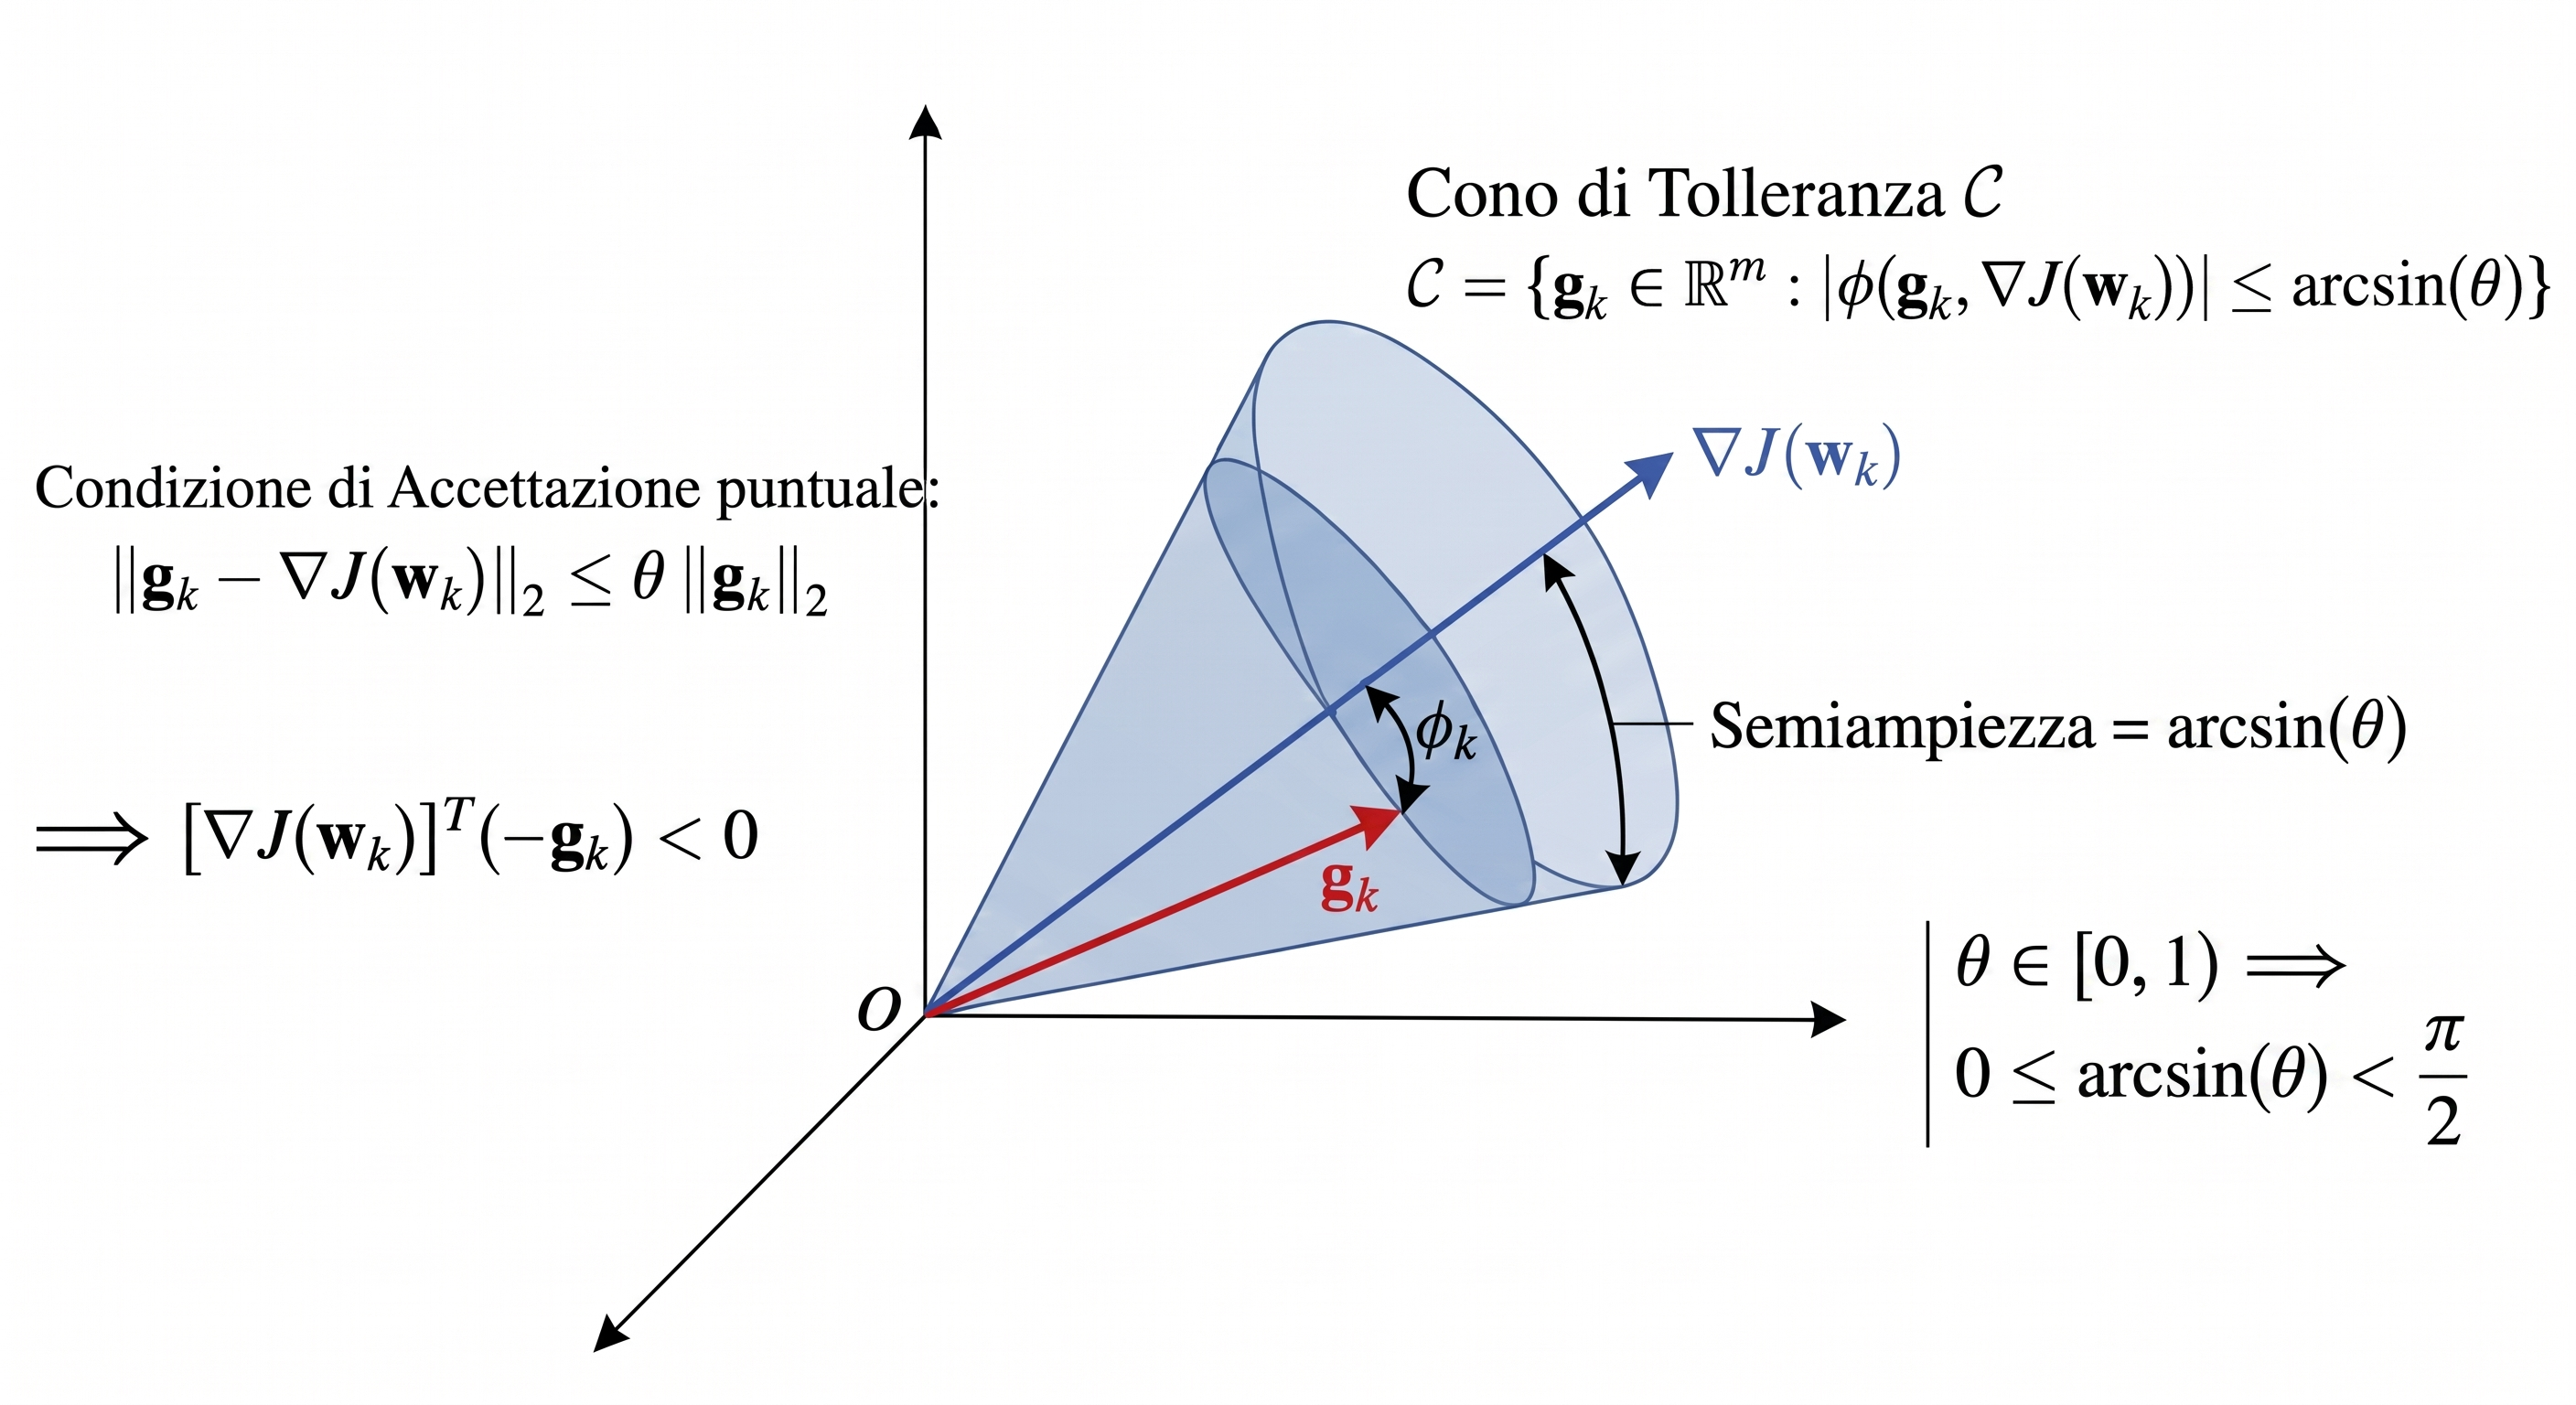
\includegraphics[width=0.68\textwidth]{conodiscesa2.jpeg}
\caption{Rappresentazione geometrica della condizione di discesa: se il
gradiente stimato $g_k$ giace nel cono di tolleranza attorno al gradiente
esatto $\nabla J(w_k)$, con errore $\|e_k\| = \|g_k - \nabla J(w_k)\| \le
\theta\|g_k\|$, allora $-g_k$ \`e una direzione di discesa per $J$.}
\label{fig:cono}
\end{figure}

\paragraph{Dimostrazione:}\label{sec:cono-dimostrazione}
Per dimostrare il fatto che $g_k$ debba essere in norma vicino al gradiente, possiamo semplicemente prendere le disuguaglianze del Lemma~\ref{lem:accuratezza} (dimostrate nella Sezione~\ref{sec:convergenza-deterministica}); poi, per trovare l'angolo, prendiamo la disuguaglianza che abbiamo ottenuto per il doppio prodotto scalare tra il gradiente di $J(w_k)$ e $g_k$ durante la dimostrazione del Lemma~\ref{lem:accuratezza}. Da lì sostituiamo la definizione di prodotto scalare e isoliamo il coseno, ottenendo un quoziente con una somma di quadrati al numeratore. Da quella somma di quadrati possiamo indebolire il termine, minorando tale somma con $2AB$ (grazie a $A^2+B^2 \ge 2AB$), e infine, dall'identità fondamentale $\sin^2\varphi+\cos^2\varphi=1$, esprimiamo il seno in funzione del coseno, $\sin\varphi=\sqrt{1-\cos^2\varphi}$, per concludere $\sin\varphi \le \theta$. \newline
Poich\'e il gradiente della popolazione totale $\nabla J(w_k)$ \`e ignoto, non \`e possibile valutare questa condizione in modo deterministico a ogni iterazione. \'E importante distinguere due livelli: la condizione puntuale $\|g_k - \nabla J(w_k)\| \le \theta\|g_k\|$ \`e quella usata nel Teorema deterministico per garantire la discesa a ogni passo; la Condizione di Controllo della Varianza (CCV) che introdurremo tra poco \`e invece una condizione in aspettativa, sufficiente per l'analisi di convergenza in media ma non una garanzia puntuale. Il mini batch $\mathcal{S}_k$ viene estratto casualmente dal dataset, rendendo $g_k$ una variabile aleatoria con $\E_{\mathcal{S}_k}[g_k] = \nabla J(w_k)$. Passare dal controllo dell'errore puntuale $\|g_k - \nabla J(w_k)\|$ al controllo del suo valore atteso permette di aggirare l'ignoranza su $\nabla J(w_k)$:
\begin{align*}
\mathbb{E}_{\mathcal{S}_k}\left[\|g_k - \mathbb{E}_{\mathcal{S}_k}[g_k]\|_2^2\right]
&= \mathbb{E}_{\mathcal{S}_k}\left[\sum_{j=1}^{m} \left(g_k^{(j)} - \mathbb{E}_{\mathcal{S}_k}[g_k^{(j)}]\right)^2\right] \\
&= \sum_{j=1}^{m} \mathbb{E}_{\mathcal{S}_k}\left[\left(g_k^{(j)} - \mathbb{E}_{\mathcal{S}_k}[g_k^{(j)}]\right)^2\right] \\
&= \sum_{j=1}^{m} \mathrm{Var}_{\mathcal{S}_k}\left(g_k^{(j)}\right)
= \left\|\mathrm{Var}_{\mathcal{S}_k}(g_k)\right\|_1.
\end{align*}

\paragraph{Decomposizione della varianza dello stimatore.}

Definiamo la varianza della popolazione (vettore):
\[
\begin{gathered}
\mathcal{V}
:= \mathbb{E}_{I}\left[ \left( \nabla \ell(w_k; I) - \mathbb{E}_{I}[\nabla \ell(w_k; I)] \right)^{2} \right] \\
= \Var_{I}\bigl(\nabla \ell(w_k; I)\bigr) 
= \frac{1}{N}\sum_{i=1}^{N}\bigl(\nabla \ell(w_k; i) - \nabla J(w_k)\bigr)^2 \in \mathbb{R}^m,
\end{gathered}
\]
dove il quadrato è inteso componente per componente, e distinguiamo $I$ variabile aleatoria distribuita uniformemente in $\{1,\dots,N\}$ con $i$ realizzazione di tale variabile.

\paragraph{Caso con reinserimento (indipendenza):}
\[
\begin{gathered}
  \Var(g_k) = \Var\!\left(\frac{1}{n_k}\sum_{i\in S_k}\nabla\ell(w_k;i)\right)
  = \frac{1}{n_k^2}\sum_{i\in S_k}\Var(\nabla\ell(w_k;i)) \\
  = \frac{1}{n_k^2}\underbrace{\Var(\nabla\ell(w_k;i))+\dots+\Var(\nabla\ell(w_k;i))}_{n_k \text{ volte}}
  = \frac{\mathcal{V}}{n_k}.
\end{gathered}
\]
Anche qui la divisione va fatta componente per componente, siccome $\mathcal{V}$ è un vettore.

\paragraph{Caso senza reinserimento (dipendenza):}
\[
  \Var\!\left(\nabla J_{S_k}(w_k)\right) = \frac{\mathcal{V}}{n_k}\cdot\frac{N-n_k}{N-1}.
\]
La dimostrazione del fattore che si aggiunge qui è riportata nell'appendice.
Per $N \gg n_k$ (condizione tipica nel Machine Learning), il fattore di correzione $\frac{N-n_k}{N-1}$ è circa $1$, quindi $\Var(g_k) \approx \mathcal{V}/n_k$: la condizione esatta si semplifica nella forma pratica riportata sotto.

Poich\'e $\mathcal{V}$ \`e ignoto, lo sostituiamo con la sua stima campionaria sul batch corrente:
\[
  \widehat{\mathcal{V}} := \Var_{i \in S_k}\bigl(\nabla \ell(w_k;i)\bigr)
  = \frac{1}{n_k-1}\sum_{i\in S_k}\bigl(\nabla \ell(w_k;i) - \nabla J_{S_k}(w_k)\bigr)^2.
\]

Otteniamo cos\`i la Condizione di Controllo della Varianza (CCV):

\begin{thmbox}
  \[
    \frac{\|\widehat{\mathcal{V}}\|_1}{n_k} \;\leq\; \theta^2 \|\nabla J_{\mathcal{S}_k}(w_k)\|_2^2,
  \]
  dove:
  \begin{itemize}
    \setlength{\itemsep}{0pt}\setlength{\topsep}{2pt}\setlength{\parskip}{0pt}
    \item $\|\cdot\|_1$ somma le varianze componente per componente,
    \item $\theta \in (0,1)$ \`e la tolleranza impostata dall'utente,
    \item $n_k$ \`e la dimensione del batch corrente.
  \end{itemize}
  Questa \`e la forma pratica per $N \gg n_k$ (corrispondente al limite $N\to\infty$ della condizione esatta che include il fattore $\frac{N-n_k}{N-1}$ derivata sopra). La condizione verifica che la varianza stimata dello stimatore sia sufficientemente piccola rispetto al gradiente corrente. Se non \`e soddisfatta, si aumenta $n_k$.
\end{thmbox}
\begin{notebox}

Dalla condizione di discesa \eqref{eq:discesa} sappiamo che, per garantire che $-g_k$ sia una direzione di discesa, dobbiamo avere $\|e_k\|_2 \le \theta\,\|g_k\|_2$, con $e_k := g_k - \nabla J(w_k)$. Elevando al quadrato:
\[
\|e_k\|_2^2 \;\le\; \theta^2\, \|g_k\|_2^2.
\]
Poiché $\nabla J(w_k)$ è ignoto, non possiamo calcolare $\|e_k\|_2^2$ esattamente. Tuttavia, poiché $\mathbb{E}[g_k] = \nabla J(w_k)$, si ha:
\[
\mathbb{E}\left[\|e_k\|_2^2\right] = \mathbb{E}\left[\|g_k - \mathbb{E}[g_k]\|_2^2\right] = \|\mathrm{Var}(g_k)\|_1.
\]
Stimando $\|\mathrm{Var}(g_k)\|_1 \approx \frac{\|\widehat{\mathcal{V}}\|_1}{n_k}$, la disuguaglianza in valore atteso diventa esattamente la CCV:
\[
\frac{\|\widehat{\mathcal{V}}\|_1}{n_k} \;\le\; \theta^2\, \|g_k\|_2^2.
\]
Il parametro $\theta$ controlla la tolleranza sull'errore relativo $\|e_k\|/\|g_k\|$; elevandolo al quadrato si preserva la coerenza dimensionale con la varianza (che è un errore quadratico medio).
\end{notebox}

\subsubsection{Regola di aggiornamento del batch}

Se la condizione CCV non \`e soddisfatta, si stima la nuova dimensione minima del batch. Supponendo che, per aumenti graduali, la varianza campionaria e la norma del gradiente non cambino significativamente (la stima della varianza per predire la dimensione del batch $k$ viene fatta con la varianza del batch $k-1$) si ottiene:\footnote{Nell'implementazione si aggiunge 1 per evitare che, quando il rapporto \`e esattamente intero, il batch non cresca, causando ripetute violazioni della CCV per fluttuazioni numeriche.}

\begin{definitionbox}
  Regola di Aggiornamento del Batch.
  \[
    n_{k}^{\mathrm{new}} = \left\lceil \frac{\|\widehat{\mathcal{V}}\|_1}{\theta^2 \|\nabla J_{\mathcal{S}_k}(w_k)\|_2^2} \right\rceil
  \]
  dove $\widehat{\mathcal{V}} := \Var_{i \in \mathcal{S}_k}(\nabla \ell(w_k;i))$ \`e la varianza campionaria.
  
\end{definitionbox}

\begin{notebox}
  Quando siamo lontani dal minimo, $\|\nabla J_{\mathcal{S}_k}(w_k)\|_2^2$ \`e grande: la formula di aggiornamento del batch d\`a un $n$ piccolo, quindi il batch resta piccolo. Avvicinandoci al minimo, il gradiente si azzera e il denominatore diventa piccolo: la formula impone un batch grande. \underline{Il batch cresce automaticamente dove serve precisione.}
\end{notebox}

\begin{figure}[h]
\centering
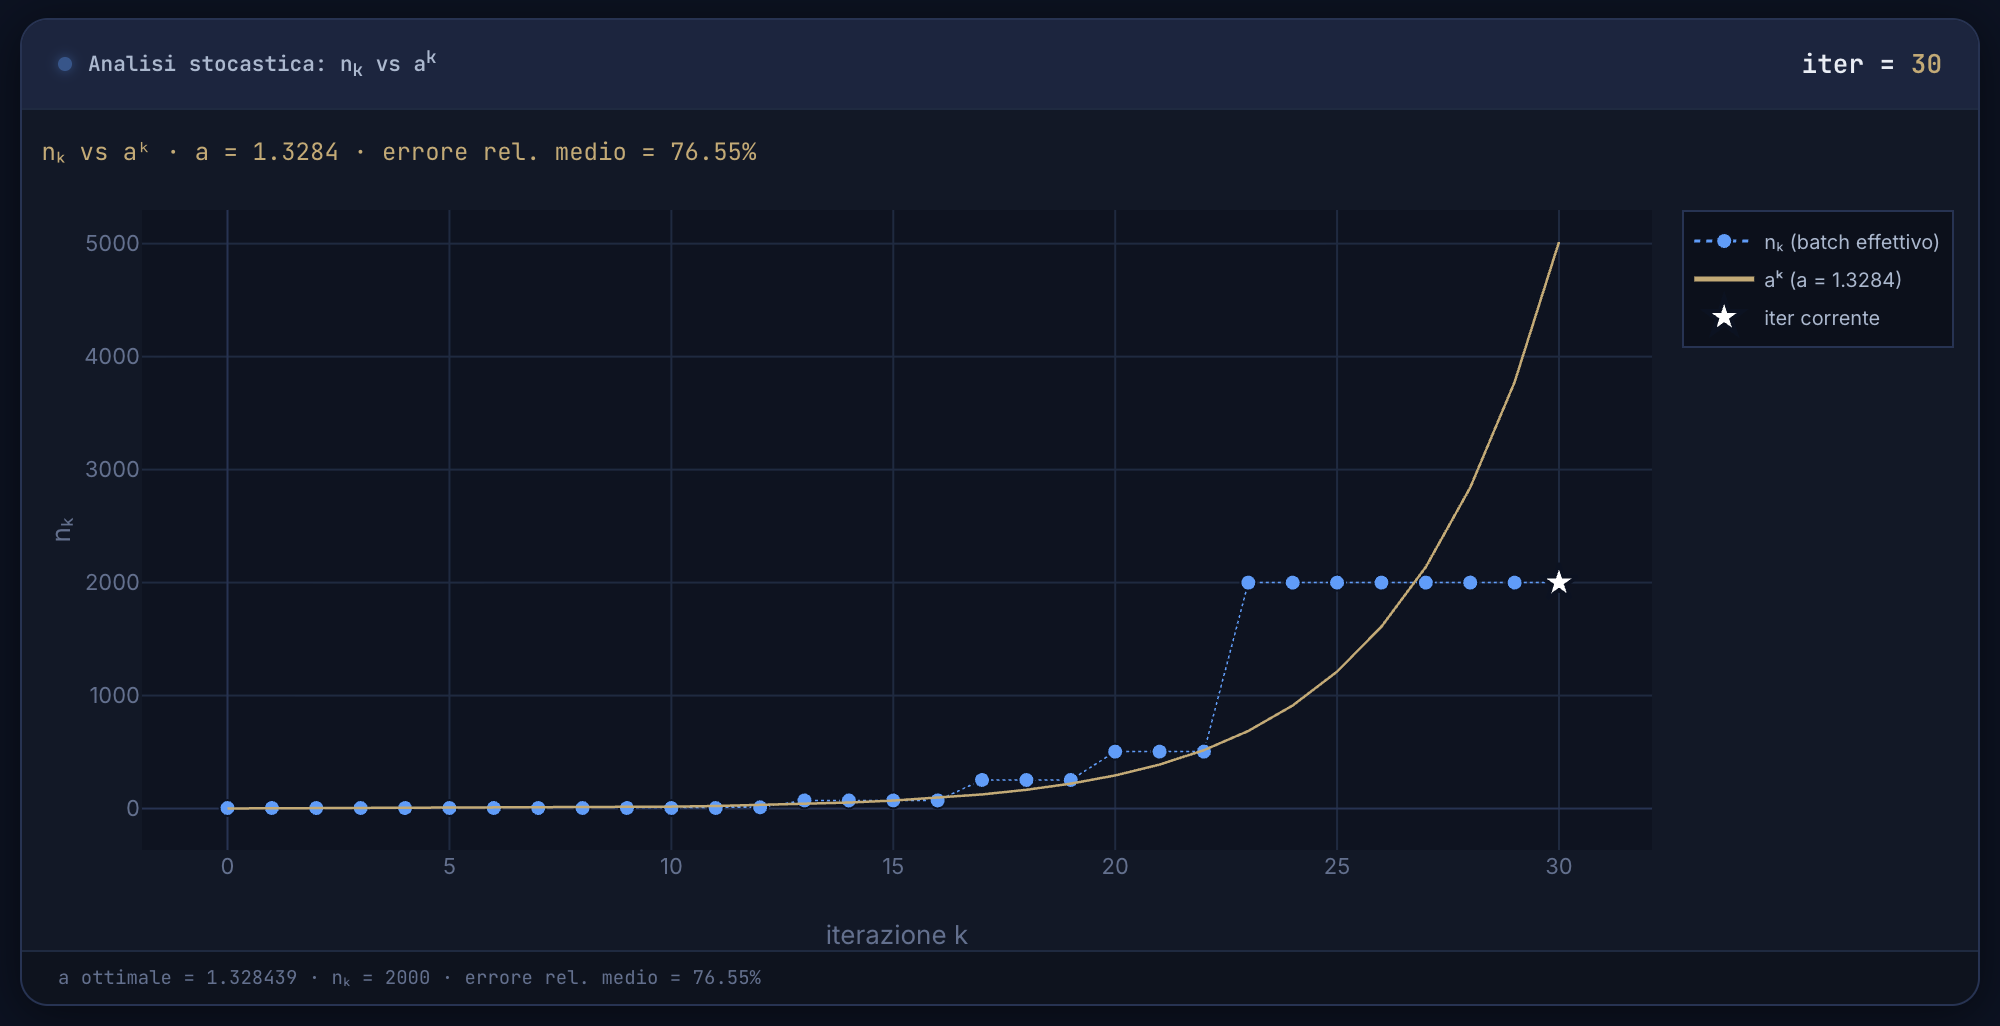
\includegraphics[width=0.78\textwidth]{figure_sim/batch_size_app.png}
\caption{Andamento della dimensione del batch $n_k$ in funzione dell'iterazione
$k$ per il metodo a campione dinamico (linea blu, con gradini in corrispondenza
delle violazioni della CCV), confrontato con la funzione esponenziale $a^k$
(curva oro). Il parametro $a > 1$ è stimato per minimi quadrati in scala
logaritmica: minimizza $\sum_k (\ln n_k - k \ln a)^2$, da cui
$\ln a = \frac{\sum_k k \ln n_k}{\sum_k k^2}$. La crescita di $n_k$ segue quindi
una legge quasi geometrica $n_k \approx a^k$, concentrando la risorsa
computazionale nelle iterazioni finali, dove il gradiente è piccolo e serve
precisione.}
\label{fig:batch_qualitativa}
\end{figure}


\subsubsection{Pseudocodice (Algoritmo)}

\begin{actionbox}
  Gradiente a Campione Dinamico\\[0.3cm]
  \textit{Input:} $w_0$ (punto iniziale), $\mathcal{S}_0$ (batch iniziale), $\theta \in (0,1)$ (tolleranza).\\[0.1cm]
  \textit{Ripeti per ogni } $k \in \mathbb{N}$ \textit{ fino a convergenza:}
  \begin{enumerate}
    \item $g_k = \nabla J_{\mathcal{S}_k}(w_k)$.
    \item $\widehat{\mathcal{V}} = \Var_{i \in \mathcal{S}_k}(\nabla \ell(w_k;i)) = \frac{1}{n_k - 1} \sum_{i \in S_k} \bigl(\nabla \ell_i(w_k) - g_k\bigr)^2
$.
    \item Se $\frac{\|\widehat{\mathcal{V}}\|_1}{n_k} > \theta^2 \|g_k\|_2^2$ aumenta il batch: $n_k \leftarrow \left\lceil \frac{\|\widehat{\mathcal{V}}\|_1}{\theta^2 \|g_k\|_2^2} \right\rceil$.
    \item Esegui una line search: trova $\alpha_k > 0$ tale che $J_{\mathcal{S}_k}(w_k - \alpha_k g_k) < J_{\mathcal{S}_k}(w_k)$.
    \item Aggiorna: $w_{k+1} = w_k - \alpha_k g_k$.
    \item Seleziona un nuovo campione $\mathcal{S}_{k+1}$ di dimensione $n_k$ (la nuova dimensione, eventualmente aumentata).
  \end{enumerate}
\end{actionbox}

% Figura 5.1 - schema a blocchi dell'algoritmo Dynamic GD (versione migliorata)
% Figura 5.1 - schema a blocchi dell'algoritmo Dynamic GD (versione migliorata)
% Figura 5.1 - schema a blocchi dell'algoritmo Dynamic GD (versione migliorata)



\newpage
\subsubsection{Convergenza deterministica}\label{sec:convergenza-deterministica}

Consideriamo l'iterazione a passo fisso
\[
w_{k+1} = w_k - \alpha g_k, \qquad \alpha = \frac{1-\theta}{L},
\]
dove $g_k$ è un'approssimazione di $\nabla J(w_k)$ che soddisfa la condizione di accuratezza
\[
\|g_k - \nabla J(w_k)\|_2 \leq \theta \|g_k\|_2, \qquad \theta \in [0,1).
\label{eq:discesa}
\]

\begin{lemma}\label{lem:accuratezza}
  Sotto la condizione di accuratezza si hanno le seguenti disuguaglianze:
  \[
  \|\nabla J(w_k)\| \leq (1+\theta)\|g_k\|, \qquad
  \|\nabla J(w_k)\| \geq (1-\theta)\|g_k\|.
  \]
  Inoltre,
  \[
  \nabla J(w_k)^T g_k \geq (1-\theta)\|g_k\|^2.
  \]
\end{lemma}
\begin{proof}
  Poniamo $e_k = g_k - \nabla J(w_k)$. Allora per definizione $\nabla J(w_k) = g_k - e_k$.
  Prima dimostrazione: $\|\nabla J(w_k)\| \leq (1+\theta)\|g_k\|$.
  Applicando la disuguaglianza triangolare $\|x+y\| \leq \|x\| + \|y\|$ con $x = g_k$ e $y = -e_k$:
  \[
  \|\nabla J(w_k)\| = \|g_k + (-e_k)\| \leq \|g_k\| + \|{-e_k}\| = \|g_k\| + \|e_k\|.
  \]
  Dalla condizione di accuratezza, $\|e_k\| \leq \theta \|g_k\|$. Sostituendo:
  \[
  \|\nabla J(w_k)\| \leq \|g_k\| + \theta \|g_k\| = (1+\theta)\|g_k\|.
  \]

  Seconda dimostrazione: $\|\nabla J(w_k)\| \geq (1-\theta)\|g_k\|$.
  Partiamo dalla disuguaglianza triangolare standard $\|a\|=\|a-b+b\| \leq \|a-b\| + \|b\|$, valida per ogni $a,b$. Ponendo $a = g_k$ e $b = e_k$:
  \[
  \|g_k\| \leq \|g_k - e_k\| + \|e_k\| = \|\nabla J(w_k)\| + \|e_k\|.
  \]
  Quindi $\|\nabla J(w_k)\| \geq \|g_k\| - \|e_k\|$. Sostituendo $\|e_k\| \leq \theta \|g_k\|$:
  \[
  \|\nabla J(w_k)\| \geq \|g_k\| - \theta \|g_k\| = (1-\theta)\|g_k\|.
  \]

  Dimostrazione di $\nabla J(w_k)^T g_k \geq (1-\theta)\|g_k\|^2$.
  Eleviamo al quadrato la condizione di accuratezza:
  \[
  \|g_k - \nabla J(w_k)\|^2 \leq \theta^2 \|g_k\|^2.
  \]
  Sviluppando il quadrato del binomio:
  \[
  \|g_k\|^2 - 2\nabla J(w_k)^T g_k + \|\nabla J(w_k)\|^2 \leq \theta^2 \|g_k\|^2.
  \]
  Isoliamo il termine con il prodotto scalare portando gli altri termini a destra:
  \[
  -2\nabla J(w_k)^T g_k \leq \theta^2 \|g_k\|^2 - \|g_k\|^2 - \|\nabla J(w_k)\|^2 = (\theta^2 - 1)\|g_k\|^2 - \|\nabla J(w_k)\|^2.
  \]
  Moltiplichiamo entrambi i membri per $-1$:
  \[
  2\nabla J(w_k)^T g_k \geq (1 - \theta^2)\|g_k\|^2 + \|\nabla J(w_k)\|^2.
  \]
  Utilizziamo ora la disuguaglianza $\|\nabla J(w_k)\| \geq (1-\theta)\|g_k\|$ dimostrata in precedenza, elevandola al quadrato:
  \[
  \|\nabla J(w_k)\|^2 \geq (1-\theta)^2 \|g_k\|^2.
  \]
  Sostituiamo questa stima nella disuguaglianza del Lemma:
  \[
  2\nabla J(w_k)^T g_k \geq (1 - \theta^2)\|g_k\|^2 + (1-\theta)^2 \|g_k\|^2.
  \]
  Raccogliamo $\|g_k\|^2$ e semplifichiamo i coefficienti:
  \[
  \begin{aligned}
  2\nabla J(w_k)^T g_k
  &\geq \bigl[(1 - \theta^2) + (1 - 2\theta + \theta^2)\bigr] \|g_k\|^2 \\
  &= \bigl[1 - \theta^2 + 1 - 2\theta + \theta^2\bigr] \|g_k\|^2
   = 2(1 - \theta) \|g_k\|^2.
  \end{aligned}
  \]
  Dividendo entrambi i membri per $2$ si ottiene la tesi:
  \[
  \nabla J(w_k)^T g_k \geq (1-\theta) \|g_k\|^2.
  \]
\end{proof}
\newpage
\begin{thmbox}
  Teorema di Convergenza Deterministica.
  Sia $J: \mathbb{R}^m \to \mathbb{R}$ una funzione $\lambda$-fortemente convessa ($\nabla^2 J(w) \succeq \lambda I$ per ogni $w$) e con gradiente $L$-Lipschitz ($\nabla^2 J(w) \preceq LI$ per ogni $w$).
  Si assuma che a ogni iterazione valga la condizione di accuratezza e si scelga il passo 
  $\alpha = \dfrac{1-\theta}{L}$. Allora
  \[
  \underbrace{J(w_{k+1}) - J(w^*)}_{=: \varepsilon_{k+1}} \;\leq\; 
  \left(1 - \frac{(1-\theta)\lambda}{L}\right) \underbrace{\bigl(J(w_k) - J(w^*)\bigr)}_{=: \varepsilon_k}.
  \]
  Di conseguenza:
  \begin{itemize}
    \item Il fattore di riduzione per iterazione \`e $\rho = 1 - \dfrac{(1-\theta)\lambda}{L} \in (0,1)$;
    \item Il numero di iterazioni per ottenere $J(w_k) - J(w^*) \le \varepsilon$ \`e al pi\`u
    \[
    k \;\ge\; \frac{L}{(1-\theta)\lambda}\,\log\!\left(\frac{J(w_0)-J(w^*)}{\varepsilon}\right)
    = O\!\left(\frac{L}{\lambda}\log\frac{1}{\varepsilon}\right).
    \]
  \end{itemize}
\end{thmbox}

\begin{notebox}
  Confronto con il risultato di Nocedal e Wright~\cite{nocedal2006}.
  Il fattore di contrazione qui ottenuto è $1 - \dfrac{(1-\theta)\lambda}{L}$, mentre Nocedal e Wright~\cite{nocedal2006} dimostrano $1 - \dfrac{(1-\theta)\lambda}{2L}$ (eq.~4.9). Ora $1 - \dfrac{(1-\theta)\lambda}{L} < 1 - \dfrac{(1-\theta)\lambda}{2L}$, cioè abbiamo un fattore di contrazione più piccolo (convergenza più rapida). Esso è dovuto all'uso della disuguaglianza di Polyak--Lojasiewicz nella forma forte $\|\nabla J(w)\|^2 \ge 2\lambda J(w)$ (dimostrata nell'appendice~\ref{app:pl}), invece della forma più debole $\|\nabla J(w)\|^2 \ge \lambda(J(w)-J(w_*))$ (eq.~4.4--4.5) utilizzata da Nocedal e Wright~\cite{nocedal2006}. La forma più forte è resa possibile dall'ipotesi di convessità forte ($\nabla^2 J \succeq \lambda I$), che implica direttamente $\|\nabla J(w)\|^2 \ge 2\lambda J(w)$ quando $J(w_*)=0$.
\end{notebox}

\begin{proof}
  Per semplificare poniamo $J(w^*) = 0$ (altrimenti si definisce $\tilde J(w) = J(w) - J(w^*)$, che soddisfa le stesse ipotesi di convessità e ha minimo nullo).

  Per la $L$-lipschitzianit\`a del gradiente, vale la seguente maggiorazione (conseguenza del teorema di Taylor con resto di Lagrange):
  \[
  J(w_{k+1}) \le J(w_k) + \nabla J(w_k)^T(w_{k+1} - w_k) + \frac{L}{2}\|w_{k+1} - w_k\|^2.
  \]
  Sostituendo $\alpha = \frac{1-\theta}{L}$ e $w_{k+1} = w_k - \alpha g_k \Rightarrow w_{k+1} - w_k =  - \alpha g_k$:
  \[
  J(w_{k+1}) \le J(w_k) - \frac{1-\theta}{L}\nabla J(w_k)^T g_k + \frac{L}{2}\left(\frac{1-\theta}{L}\right)^2\|g_k\|^2.
  \]
  Semplifichiamo il coefficiente del termine quadratico:
  \[
  \frac{L}{2}\left(\frac{1-\theta}{L}\right)^2 = \frac{L}{2} \cdot \frac{(1-\theta)^2}{L^2} = \frac{(1-\theta)^2}{2L}.
  \]
  Quindi:
  \[
  J(w_{k+1}) \le J(w_k) \underbrace{- \frac{1-\theta}{L}\nabla J(w_k)^T g_k + \frac{(1-\theta)^2}{2L}\|g_k\|^2}_{:=S}.
  \]

  Moltiplichiamo la disuguaglianza del Lemma per $\frac{1-\theta}{2L}$:
  \[
  \frac{1-\theta}{2L} \cdot 2\nabla J(w_k)^T g_k \;\ge\; \frac{1-\theta}{2L}\Bigl[(1-\theta^2)\|g_k\|^2 + \|\nabla J(w_k)\|^2\Bigr].
  \]
  Semplificando il membro sinistro:
  \[
  \frac{1-\theta}{L}\nabla J(w_k)^T g_k \;\ge\; \frac{(1-\theta)(1-\theta^2)}{2L}\|g_k\|^2 + \frac{1-\theta}{2L}\|\nabla J(w_k)\|^2.
  \]

  Riorganizziamo la disuguaglianza appena scritta per isolare $-\frac{1-\theta}{L}\nabla J(w_k)^T g_k$, che compare nella definizione di $S$:
  \[
  -\frac{1-\theta}{L}\nabla J(w_k)^T g_k \;\le\; -\frac{(1-\theta)(1-\theta^2)}{2L}\|g_k\|^2 - \frac{1-\theta}{2L}\|\nabla J(w_k)\|^2.
  \]

  Inseriamo questa disuguaglianza nella definizione di $S$:
  \[
  J(w_{k+1}) \le J(w_k) - \frac{(1-\theta)(1-\theta^2)}{2L}\|g_k\|^2 - \frac{1-\theta}{2L}\|\nabla J(w_k)\|^2 + \frac{(1-\theta)^2}{2L}\|g_k\|^2.
  \]

  Raccogliamo i coefficienti di $\|g_k\|^2$:
  \[
  -\frac{(1-\theta)(1-\theta^2)}{2L} + \frac{(1-\theta)^2}{2L}
  = -\frac{1-\theta}{2L}\Bigl[(1-\theta^2) - (1-\theta)\Bigr].
  \]
  Calcoliamo la differenza tra parentesi:
  \[
  (1-\theta^2) - (1-\theta) = 1 - \theta^2 - 1 + \theta = \theta - \theta^2 = \theta(1-\theta).
  \]
  Quindi:
  \[
  -\frac{1-\theta}{2L} \cdot \theta(1-\theta) = -\frac{\theta(1-\theta)^2}{2L}.
  \]

  La disuguaglianza diventa:
  \[
  J(w_{k+1}) \le J(w_k) - \frac{\theta(1-\theta)^2}{2L}\|g_k\|^2 - \frac{1-\theta}{2L}\|\nabla J(w_k)\|^2.
  \]

  Poiché $\frac{\theta(1-\theta)^2}{2L}\|g_k\|^2 \ge 0$, il termine $-\frac{\theta(1-\theta)^2}{2L}\|g_k\|^2$ è minore o uguale a zero, trascurarlo può solo aumentare il membro destro e la disuguaglianza rimane valida:
  \[
  J(w_{k+1}) \le J(w_k) - \frac{1-\theta}{2L}\|\nabla J(w_k)\|^2.
  \]
  Infine, dalla disuguaglianza di convessità forte dimostrata nell'Appendice~\ref{app:pl},
  \[
  \|\nabla J(w_k)\|^2 \ge 2\lambda J(w_k) \qquad (\text{valida con } J(w_*)=0),
  \]
  si ottiene:
\[
S \le -\frac{1-\theta}{2L} \cdot 2\lambda J(w_k)
= -\frac{\lambda(1-\theta)}{L} J(w_k).
\]
Sostituendo nella disuguaglianza che definisce $S$:
\[
J(w_{k+1}) \le J(w_k) - \frac{\lambda(1-\theta)}{L} J(w_k)
= \left(1 - \frac{\lambda(1-\theta)}{L}\right) J(w_k).
\]

Applicando la disuguaglianza appena dimostrata ricorsivamente:
\[
J(w_k) \le \rho^k J(w_0), \qquad \text{dove } \rho = 1 - \frac{\lambda(1-\theta)}{L}.
\]
Poiché $\theta \in [0,1)$, $\lambda > 0$ e $L > 0$, si ha $\rho \in (0,1)$.

Imponiamo $J(w_k) \le \varepsilon$:
\[
\rho^k J(w_0) \le \varepsilon \quad\Longrightarrow\quad k \ge \frac{\log(J(w_0)/\varepsilon)}{\log(1/\rho)}.
\]
Usando $\log(1/\rho) \ge 1-\rho$:
\[
1 - \rho = \frac{\lambda(1-\theta)}{L},
\]
quindi:
\[
k \ge \frac{L}{\lambda(1-\theta)}\,\log\!\left(\frac{J(w_0)}{\varepsilon}\right).
\]

Questa è la stima del numero di iterazioni necessarie per ridurre l'errore al di sotto di $\varepsilon$.
\end{proof}


\subsubsection{Analisi Stocastica e Complessità del Metodo}

Nell'analisi deterministica abbiamo assunto la condizione di accuratezza
\[
\|g_k - \nabla J(w_k)\|_2 \le \theta \|g_k\|_2, \qquad \theta \in [0,1), \tag{5.1}
\]
garantendo che \(-g_k\) sia una direzione di discesa per \(J\) e stabilendo la convergenza lineare (Teorema di Convergenza Deterministica).

Nel caso stocastico, \(g_k = \nabla J_{\mathcal{S}_k}(w_k)\) è calcolato su un campione casuale \(\mathcal{S}_k\) di dimensione \(n_k\), rendendo \(g_k\) una variabile aleatoria. La condizione (5.1) non può essere garantita con probabilità 1 per ogni iterazione. Dobbiamo quindi sviluppare un'analisi in aspettativa, tenendo conto che \(n_k\) può variare nel corso delle iterazioni.

\paragraph{Impostazione del problema stocastico}

Definiamo
\[
g_k := \nabla J_{\mathcal{S}_k}(w_k) = \frac{1}{n_k}\sum_{i\in \mathcal{S}_k}\nabla \ell(w_k;i), \qquad n_k := |\mathcal{S}_k|. \tag{5.2}
\]
Per ogni \(w_k\) fissato, \(g_k\) è uno stimatore non distorto:
\[
\mathbb{E}[g_k \mid w_k] = \nabla J(w_k). \tag{5.3}
\]

Introduciamo l'ipotesi fondamentale di limitatezza della varianza dei gradienti individuali. Si noti che questa \`e un'ipotesi forte, necessaria per l'analisi di complessit\`a teorica; in pratica pu\`o essere rilassata, ad esempio richiedendo la limitatezza solo in un intorno del minimo o utilizzando stime locali della varianza.

\begin{notebox}
  Ipotesi di limitatezza della varianza.
   \(\exists \omega \in \mathbb{R},\omega > 0\) tale che \(\forall w_k\),
  \[
  \|\mathrm{Var}(\nabla \ell(w_k;I))\|_1 \le \omega, \tag{5.4}\label{eq:var_bound}
  \]
  dove \(\mathrm{Var}(\nabla \ell(w_k;I)) := \mathbb{E}_I[(\nabla \ell(w_k;I) - \nabla J(w_k))^2]\) è inteso componente per componente.
\end{notebox}


Dal Lemma~\ref{lem:accuratezza} abbiamo $\|\nabla J(w_k)\|\ge(1-\theta)\|g_k\|$,
da cui
\[
\|g_k\|^2\le\frac{1}{(1-\theta)^2}\|\nabla J(w_k)\|^2.
\]
Dall'Appendice~\ref{app:pl} (disuguaglianza $J(w)\ge\frac{\lambda}{2L^2}\|\nabla J(w)\|^2$)
otteniamo $\|\nabla J(w_k)\|^2\le\frac{2L^2}{\lambda}J(w_k)$.
Combinando con la convergenza lineare del Teorema di Convergenza Deterministica,
$J(w_k)\le\bigl(1-\frac{(1-\theta)\lambda}{L}\bigr)^k J(w_0)$, segue
\[
\|g_k\|^2\le\frac{1}{(1-\theta)^2}\frac{2L^2}{\lambda}J(w_k)
\le\frac{1}{(1-\theta)^2}\frac{2L^2 J(w_0)}{\lambda}
\left(1-\frac{(1-\theta)\lambda}{L}\right)^k.
\tag{5.5}\label{eq:bound_gk}
\]
Va osservato che questo bound ha natura circolare: la convergenza lineare del Teorema di Convergenza Deterministica, usata nella (5.5), richiede a sua volta che la CCV sia soddisfatta a ogni iterazione, ed è proprio questo che si intende garantire con la scelta di $n_k$. La (5.5) va quindi intesa come una stima guida/euristica per la scelta di $n_k$, non come una derivazione rigorosa, in analogia con quanto fatto nel lavoro originale~\cite{byrd2012}.
Questo bound adotta il tasso deterministico $\rho=1-\frac{(1-\theta)\lambda}{L}$ usato nel teorema precedente.  Si noti che questo tasso è più favorevole (più rapido) rispetto a quello ottenuto da Byrd et al.~\cite{byrd2012}, che presentano un fattore $1/2$ aggiuntivo a denominatore a causa dell'uso di una disuguaglianza più debole.
Dalla Condizione di Controllo della Varianza (CCV):
\[
\frac{\|\overbrace{\mathrm{Var}_{i\in\mathcal{S}_k}(\nabla \ell(w_k;i))}^{\widehat{\mathcal{V}}}\|_1}{n_k} \le \theta^2 \|g_k\|^2. \tag{5.6}\]
Per garantire la (5.6) in media, dobbiamo scegliere \(n_k\) sufficientemente grande. Usando l'ipotesi (5.4), la condizione (5.6) è sicuramente soddisfatta se
\[
\frac{\omega}{n_k} \le \theta^2 \|g_k\|^2,
\]
ovvero se
\[
n_k \;\ge\; \frac{\omega}{\theta^2 \|g_k\|^2}. \tag{5.7}
\]
Osserviamo che la (5.5) fornisce un bound superiore su \(\|g_k\|^2\) che decresce geometricamente con tasso \(\rho = 1-(1-\theta)\lambda/L\). Poiché nella (5.7) la dimensione del batch è inversamente proporzionale a \(\|g_k\|^2\), al restringersi del gradiente \(n_k\) deve crescere per evitare che il rumore domini la discesa. Per stimare la velocità di crescita necessaria, usiamo il bound (5.5) per valutare il tasso massimo con cui il denominatore di (5.7) può restringersi: sostituendo la (5.5) nella (5.7) si ottiene una condizione guida sulla crescita di \(n_k\),
\[
n_k \;\ge\; \frac{\omega}{\theta^2 \cdot \frac{1}{(1-\theta)^2}\frac{2L^2 J(w_0)}{\lambda}\left(1 - \frac{(1-\theta)\lambda}{L}\right)^k}
\;=\; \frac{\omega (1-\theta)^2 \lambda}{\theta^2 2L^2 J(w_0)}
\left(1 - \frac{(1-\theta)\lambda}{L}\right)^{-k}. \tag{5.8}
\]
Pertanto, per far decadere il rumore almeno alla stessa velocità con cui l'errore deterministico si riduce, \(n_k\) deve crescere geometricamente come
\[
n_k \;\ge\; O\!\left(\left(1 - \frac{(1-\theta)\lambda}{L}\right)^{-k}\right).
\]
Nell'analisi stocastica imponiamo quindi:
\[
n_k = \lceil a^k \rceil, \qquad a > 1. \tag{5.9}
\]

Le ipotesi si dividono in due categorie complementari:
\begin{itemize}
    \item Ipotesi strutturali su \(J\) (\(\lambda I \preceq \nabla^2 J(w) \preceq LI\)): garantiscono la convergenza lineare se la direzione di discesa è accurata (Teorema di Convergenza Deterministica), e forniscono la maggiorazione di Taylor (A.12), che sarà usata per derivare la disuguaglianza di convergenza in aspettativa.
    \item Ipotesi stocastica (5.4): garantisce che la varianza dello stimatore \(g_k\) decada come \(\|\mathrm{Var}(g_k)\|_1 \le \omega/n_k\), rendendo il rumore controllabile aumentando il batch.
\end{itemize}

\paragraph{Iterazione stocastica a passo fisso}

Consideriamo l'iterazione
\[
w_{k+1} = w_k - \frac{1}{L} g_k. \tag{5.10}
\]
Nell'analisi stocastica si adotta il passo $1/L$, più lungo del passo deterministico $(1-\theta)/L$ poiché il fattore $(1-\theta)$ non è necessario quando il controllo dell'errore è affidato alla crescita del batch. Questo produce un tasso di contrazione deterministico $\alpha = 1-\lambda/L$ più piccolo rispetto a $1-(1-\theta)\lambda/L$, e quindi un reciproco $(1-\lambda/L)^{-1}$ più grande: il vincolo su $a$ ammette un bound superiore più alto.

Usando la (A.12) con \(y = w_{k+1}\) e \(w = w_k\):
\[
J(w_{k+1}) \le J(w_k) + \nabla J(w_k)^T (w_{k+1} - w_k) + \frac{L}{2}\|w_{k+1} - w_k\|^2. \tag{5.11}
\]
Sostituendo \(w_{k+1} - w_k = -\frac{1}{L}g_k\):
\[
J(w_{k+1}) \le J(w_k) - \frac{1}{L}\nabla J(w_k)^T g_k + \frac{1}{2L}\|g_k\|^2. \tag{5.12}
\]

Passando al valore atteso condizionato a \(w_k\):
\[
\mathbb{E}[J(w_{k+1}) \mid w_k] \le J(w_k) - \frac{1}{L}\nabla J(w_k)^T \mathbb{E}[g_k \mid w_k] + \frac{1}{2L}\mathbb{E}[\|g_k\|^2 \mid w_k].
\]
Usando (5.3):
\[
\mathbb{E}[J(w_{k+1}) \mid w_k] \le J(w_k) - \frac{1}{L}\|\nabla J(w_k)\|^2 + \frac{1}{2L}\mathbb{E}[\|g_k\|^2 \mid w_k]. \tag{5.13}
\]

Per esprimere \(\mathbb{E}[\|g_k\|^2 \mid w_k]\), utilizziamo l'identità \(\mathbb{E}[\|X\|^2] = \|\mathrm{Var}(X)\|_1 + \|\mathbb{E}[X]\|^2\) (valida componente per componente). Applicandola a \(X = g_k\):
\[
\mathbb{E}[\|g_k\|^2 \mid w_k] = \|\mathrm{Var}(g_k)\|_1 + \|\nabla J(w_k)\|^2. \tag{5.14}
\]
Sostituendo in (5.13):
\[
\mathbb{E}[J(w_{k+1}) \mid w_k] \le J(w_k) - \frac{1}{2L}\|\nabla J(w_k)\|^2 + \frac{1}{2L}\|\mathrm{Var}(g_k)\|_1. \tag{5.15}
\]

Dalla formula per la varianza di una media campionaria (derivata in precedenza) e dall'ipotesi (5.4):
\[
\|\mathrm{Var}(g_k)\|_1 \le \frac{\|\mathrm{Var}(\nabla \ell(w_k;i))\|_1}{n_k} \le \frac{\omega}{n_k}. \tag{5.16}
\]
Sostituendo in (5.15):
\[
\mathbb{E}[J(w_{k+1}) \mid w_k] \le J(w_k) - \frac{1}{2L}\|\nabla J(w_k)\|^2 + \frac{\omega}{2L n_k}. \tag{5.17}
\]

Dalla \(\lambda\)-convessità forte di \(J\) (disuguaglianza di PL dimostrata nell'Appendice~\ref{app:pl}):
\[
\|\nabla J(w_k)\|^2 \ge 2\lambda (J(w_k) - J(w_*)). \tag{5.18}
\]
Sostituendo in (5.17):
\[
\mathbb{E}[J(w_{k+1}) - J(w_*) \mid w_k] \le \left(1 - \frac{\lambda}{L}\right)(J(w_k) - J(w_*)) + \frac{\omega}{2L n_k}. \tag{5.19}
\]
Prendendo il valore atteso totale e ponendo \(\varepsilon_k := \mathbb{E}[J(w_k) - J(w_*)]\):
\[
\varepsilon_{k+1} \le \left(1 - \frac{\lambda}{L}\right)\varepsilon_k + \frac{\omega}{2L n_k}. \tag{5.20}
\]
Questa è l'equazione fondamentale che governa la convergenza in aspettativa.

Possiamo ora enunciare il teorema di convergenza in aspettativa.

\begin{thmbox}
Teorema 5.1 (Convergenza in aspettativa).
Posto $\alpha := 1-\frac{\lambda}{L}$ e $\beta := \frac{\omega}{2L}$, per ogni $k\ge 0$ vale
\[
\mathbb{E}[J(w_k)-J(w_*)] \;\le\; \alpha^k\varepsilon_0
+ \beta a\,\frac{\alpha^k-a^{-k}}{\alpha a-1},
\tag{5.21}
\]
dove il rapporto va inteso nel senso dei limiti se $\alpha a=1$.
Di conseguenza, posto $\rho:=\max\{\alpha,1/a\}$, se $a>1$ si ha $\rho<1$ e
esiste una costante $C=C(\varepsilon_0,\omega,\lambda,L,a)$ tale che
\[
\mathbb{E}[J(w_k)-J(w_*)]\le C\rho^k\quad\forall k\ge0.
\]
\end{thmbox}

\begin{notebox}
  Differenza rispetto al lavoro originale~\cite{byrd2012} (Teorema 4.2).
  Il paper ottiene \(\rho = \max\{1-\lambda/(4L),\,1/a\}\) e \(C = \max\{J(w_0)-J(w_*),\,2\omega/\lambda\}\) tramite un argomento induttivo che introduce un fattore \(\tfrac{1}{2}\) aggiuntivo. La dimostrazione qui presentata ottiene invece \(\rho = \max\{1-\lambda/L,\,1/a\}\) risolvendo esplicitamente la ricorrenza, il che dà un tasso deterministico \(\alpha = 1-\lambda/L\) più conservativo. Di conseguenza, l'intervallo ammissibile per \(a\) nel Corollario~5.2 è \((1,\,(1-\lambda/L)^{-1}]\) anziché \((1,\,(1-\lambda/(4L))^{-1}]\) come nel paper.
\end{notebox}

\begin{proof}

\text{Iterazione della ricorrenza e forma chiusa}

Dalla (5.20) possiamo esplicitare l'andamento di $\varepsilon_k$. Scriviamo i primi passi:

\begin{align*}
\varepsilon_1 &\le \alpha \varepsilon_0 + \beta, \\
\varepsilon_2 &\le \alpha \varepsilon_1 + \beta a^{-1}
\le \alpha(\alpha \varepsilon_0 + \beta)+\beta a^{-1}
= \alpha^2 \varepsilon_0 + \alpha\beta + \beta a^{-1}, \\
\varepsilon_3 &\le \alpha \varepsilon_2 + \beta a^{-2}
\le \alpha\bigl(\alpha^2 \varepsilon_0 + \alpha\beta + \beta a^{-1}\bigr) + \beta a^{-2} \\
&= \alpha^3 \varepsilon_0 + \alpha^2\beta + \alpha\beta a^{-1} + \beta a^{-2}.
\end{align*}

Il pattern generale è

\begin{equation}
\varepsilon_k \le \alpha^k \varepsilon_0 + \beta \sum_{j=0}^{k-1} \alpha^{k-1-j} a^{-j}. \tag{5.22}
\end{equation}

Calcoliamo la somma geometrica finita:

\[
S_k := \sum_{j=0}^{k-1} \alpha^{k-1-j} a^{-j}.
\]

Ponendo $i = k-1-j$, si ha:

\[
S_k = \sum_{i=0}^{k-1} \alpha^{i} a^{-(k-1-i)}
= a^{-(k-1)} \sum_{i=0}^{k-1} (\alpha a)^i.
\]

Se $\alpha a \neq 1$, la progressione geometrica dà:

\begin{equation}
S_k = a^{-(k-1)} \frac{1 - (\alpha a)^k}{1 - \alpha a}
= \frac{a(\alpha^k - a^{-k})}{\alpha a - 1}. \tag{5.23}
\end{equation}

Sostituendo (5.23) in (5.22) si ottiene la forma chiusa:

\begin{equation}
\varepsilon_k \le \alpha^k \varepsilon_0 + \beta a\,\frac{\alpha^k - a^{-k}}{\alpha a - 1}, \tag{5.24}
\end{equation}

che è la (5.24), cioè la (5.21) del teorema. Questa espressione è valida per $\alpha a \neq 1$; nel caso $\alpha a = 1$ si intende per limite e si ottiene $\varepsilon_k \le (\varepsilon_0 + \beta k/\alpha)\rho^k$ (con $\rho = \alpha$), che porta allo stesso tasso esponenziale a meno di un fattore polinomiale.

\paragraph{Deduzione del tasso di convergenza}

Dalla (5.21) possiamo ricavare il tasso di convergenza studiando il comportamento asintotico. Si presentano tre casi.

\begin{itemize}

\item Caso $\alpha a > 1$: allora $\alpha > 1/a$, quindi $\alpha^k$ decresce più lentamente di $a^{-k}$; il termine $\alpha^k$ domina. Trascurando $a^{-k}$ rispetto a $\alpha^k$:
\[
\varepsilon_k \le \alpha^k \varepsilon_0 + \frac{\beta a}{\alpha a - 1} \alpha^k
= \left(\varepsilon_0 + \frac{\beta a}{\alpha a - 1}\right) \alpha^k.
\]
Quindi $\rho = \alpha = 1 - \lambda/L$.
Possiamo trascurare il fattore $a^{-k}$ perche è un o piccolo rispetto ad $\alpha^k$: infatti $\lim_{k \to \infty} \frac{a^{-k}}{\alpha^k} = \lim_{k \to \infty} \left(\frac{1/a}{\alpha}\right)^k = \lim_{k \to \infty} \left(\frac{1}{\alpha a}\right)^k$ poiché $\alpha a > 1$, si ha $0 < \frac{1}{\alpha a} < 1 \implies \lim_{k \to \infty} \left(\frac{1}{\alpha a}\right)^k = 0 \implies \frac{a^{-k}}{\alpha^k} \to 0$

\item Caso $\alpha a < 1$: allora $\alpha < 1/a$, quindi $a^{-k}$ decresce più lentamente di $\alpha^k$; il termine $a^{-k}$ domina. Trascurando $\alpha^k$ rispetto a $a^{-k}$:
\[
\varepsilon_k \le \frac{\beta a}{1 - \alpha a} a^{-k}
= \frac{\beta a}{1 - \alpha a} \left(\frac{1}{a}\right)^k.
\]
Quindi $\rho = 1/a$.
Possiamo trascurare il fattore $\alpha^k$ perché è un $o$-piccolo rispetto a $a^{-k}$: infatti $\lim_{k \to \infty} \frac{\alpha^k}{a^{-k}}
= \lim_{k \to \infty} \frac{\alpha^k}{(1/a)^k}
= \lim_{k \to \infty} (\alpha a)^k$
poiché $0<\alpha a < 1$, si ha $0 < \alpha a < 1 \implies \lim_{k \to \infty} (\alpha a)^k = 0 \implies \frac{\alpha^k}{a^{-k}} \to 0$.
\item Caso $\alpha a = 1$: allora $\alpha = 1/a$. La somma geometrica si riduce a $S_k = k a^{-(k-1)}$, da cui:
\[
\varepsilon_k \le \alpha^k \varepsilon_0 + \beta k a^{-(k-1)} = (\varepsilon_0 + \beta k/\alpha)\rho^k,
\qquad\rho:=\alpha=1/a.
\]
Poich\'e per ogni $\rho' \in (\rho,1)$ esiste una costante $C$ (indipendente da $k$) tale che $k\rho^k \le C(\rho')^k$, la tesi vale con tasso $\rho'$.
\end{itemize}
 Quindi per $\alpha a>1$ si ottiene $\rho=\alpha$ e $C=\varepsilon_0+\frac{\beta a}{\alpha a-1}$; se $\alpha a<1$ si ottiene $\rho=1/a$ e $C=\varepsilon_0+\frac{\beta a}{1-\alpha a}$ (o, più strettamente, $C=\max\{\varepsilon_0,\frac{\beta a}{1-\alpha a}\}$).

In tutti i casi si ha:

\begin{equation}
\varepsilon_k \le C \rho^k, \qquad \rho := \max\{\alpha, 1/a\}, \tag{5.25}
\end{equation}

per una opportuna costante $C = C(\varepsilon_0, \omega, \lambda, L, a)$.


\end{proof}


\paragraph{Corollario sulla complessità totale}

\begin{corollarybox}
  Corollario 5.2 (Complessità totale).
  Supponiamo \(n_k = \lceil a^k \rceil\) con
  \[
  a \in \left(1,\; \underbrace{\left(1 - \frac{\lambda}{L}\right)^{-1}}_{1/\alpha}\right],
  \]
  e che (5.4) valga per tutti i \(w_k\). Allora il numero totale di valutazioni dei gradienti \(\nabla \ell(w;i)\) necessarie per ottenere \(\mathbb{E}[J(w_k) - J(w_*)] \le \varepsilon\) è
  \[
  O\!\left(\frac{L}{\lambda \varepsilon}\right), \tag{5.26}
  \]
  e il lavoro totale dell'algoritmo (5.10) con campionamento dinamico (5.9) è
  \[
  \mathcal{T}_{\mathrm{tot}} = O\!\left(\frac{L m}{\lambda \varepsilon} \max\left\{J(w_0) - J(w_*),\; \frac{\omega}{\lambda}\right\}\right), \tag{5.27}
  \]
  dove \(m\) è il numero di variabili.
\end{corollarybox}

\begin{proof}
Con la scelta \(a \le \alpha^{-1}\), si ha \(\rho = 1/a\). Dalla (5.21), il numero di iterazioni \(k\) necessario per ottenere \(\mathbb{E}[J(w_k) - J(w_*)] \le \varepsilon\) soddisfa \(a^k \ge C/\varepsilon\). Poiché \(\rho = 1/a\), la condizione \(C\rho^k \le \varepsilon\) equivale a \(a^k \ge C/\varepsilon\). Il numero di iterazioni necessario soddisfa quindi \(a^k = \Theta(C/\varepsilon)\). Il costo in valutazioni del gradiente è:
\[
\sum_{j=0}^{k-1} n_j \;\le\; 2\sum_{j=0}^{k-1} a^j
\;=\; 2\cdot \frac{a^k - 1}{a-1}
\;\le\; \frac{2}{a-1}\, a^k
\;=\; O\!\left(\frac{1}{\varepsilon}\right).\]
Moltiplicando per il costo \(O(m)\) di ogni gradiente si ottiene (5.27).
\end{proof}


\paragraph{Scelta di \(a\) e confronto}

Il risultato (5.27) vale se \(a\) è scelto nell'intervallo
\[
a \in \left(1,\; \left(1 - \frac{\lambda}{L}\right)^{-1}\right].
\]
Non è necessario conoscere il numero di condizionamento \(\kappa = L/\lambda\) esattamente; qualsiasi sovrastima va bene:
\[
a = \left(1 - \frac{1}{\kappa'}\right)^{-1}, \qquad \kappa' \ge \kappa. \tag{5.28}
\]

Dalla (5.27) ignorando la dipendenza dal punto iniziale (come in~\cite{bottou2008}) e assumendo il regime $\omega/\lambda \geq J(w_0)-J(w_*)$, si ottiene $\mathcal{T}_{\mathrm{tot}} = O(m\kappa\omega/\lambda\varepsilon)$, che è il bound riportato in tabella sotto.

Confrontiamo questo risultato con i bound di complessità noti per il metodo a gradiente a campione fisso e il metodo del gradiente stocastico (SGD), calcolati da Bottou e Bousquet~\cite{bottou2008}: nella tabella, lo scalare $\bar{\alpha} \in [1/2, 1]$ è il \textit{tasso di stima} del metodo a campione fisso, come definito in~\cite{bottou2008}.
\begin{table}[h]
\centering
\begin{tabular}{|l|c|}
\hline
Nome algoritmo & Bound \\
\hline
Metodo a gradiente dinamico (questo lavoro) & \(O(m\kappa \omega / \lambda \varepsilon)\) \\
Metodo a gradiente a campione fisso & \(O(m^2 \kappa\varepsilon^{-1/\bar{\alpha}} \log^2(1/\varepsilon))\) \\
Metodo del gradiente stocastico & \(O(m\bar{\nu}\kappa^2 / \varepsilon)\) \\
\hline
\end{tabular}
\caption{Bound di complessità per tre metodi. Qui \(m\) è il numero di variabili, \(\kappa = L/\lambda\), \(\omega\) e \(\bar{\nu}\) sono definiti in (5.4) e (5.29), e \(\bar{\alpha} \in [1/2, 1]\).}
\end{table}

I metodi a campione fisso e stocastico sono definiti come:
\begin{itemize}
  \item \text{Metodo a campione fisso: } \(w_{k+1} = w_k - \frac{1}{L} \frac{\sum_{i=1}^{N_\varepsilon} \nabla \ell(w_k;i)}{N_\varepsilon}\),
  \item \text{Metodo del gradiente stocastico: } \(w_{k+1} = w_k - \frac{1}{\lambda k} \nabla \ell(w_k; i_k)\),
\end{itemize}
dove \(N_\varepsilon\) specifica una dimensione del campione tale che \(\mathbb{E}[|J(w_*) - J_{\mathcal{S}}(w_*)|] < \varepsilon\) vale in aspettativa. I bound di complessità presentati in~\cite{bottou2008} ignorano l'effetto del punto iniziale \(w_0\).

Lo scalare \(\bar{\alpha} \in [1/2, 1]\), chiamato \textit{tasso di stima}~\cite{bottou2008}, dipende dalle proprietà della funzione di perdita; la costante \(\bar{\nu}\) è definita come
\[
\bar{\nu} = \mathrm{trace}(H^{-1}G), \qquad H = \nabla^2 J(w_*), \quad G = \mathbb{E}[\nabla \ell(w_*; i) \nabla \ell(w_*; i)^T]. \tag{5.29}
\]
Poiché \(H \succeq \lambda I\) e \(\omega\) è un bound per \(\|\mathrm{Var}(\nabla \ell(w_k;I))\|_1\), si ha \(\bar{\nu} \approx \omega/\lambda\). Sostituendo nel bound per SGD:
\[
O(m\bar{\nu}\kappa^2/\varepsilon) = O\!\left(\frac{m \omega \kappa^2}{\lambda \varepsilon}\right). \tag{5.30}
\]
Il bound per il metodo dinamico (5.27) è invece \(O(m\kappa\omega/(\lambda\varepsilon))\). La differenza principale è il termine \(\kappa^2\) in SGD contro \(\kappa\) nel metodo dinamico. Concludiamo che il metodo a gradiente dinamico gode di un bound di complessità competitivo con quello del metodo del gradiente stocastico, risultando particolarmente vantaggioso per problemi mal condizionati (grande \(\kappa\)).

La strategia dinamica \(n_k = \lceil a^k \rceil\) con \(a\) scelto in base a una stima (bound superiore) di \(\kappa\) garantisce un compromesso ottimale tra costo per iterazione e velocità di convergenza. In pratica, la stima di \(\kappa\) può essere sostituita da una regola euristica semplice (ad esempio, \(a=1.1\)), e l'algoritmo si adatta automaticamente.

\newpage
\subsection{Metodo di Newton-CG con Campionamento Dinamico}

Il metodo del gradiente (steepest descent) può convergere lentamente, specialmente su problemi mal condizionati; gli algoritmi che incorporano informazione di curvatura (secondo ordine) sulla funzione obiettivo possono essere molto più efficienti. In questa sezione descriviamo un metodo di Newton-CG (gradiente coniugato) Hessian free (non costruiamo e non memorizziamo esplicitamente la matrice Hessiana di $J(w)$, ma ne usiamo solo i prodotti per un vettore), che impiega tecniche di campionamento dinamico sia per il calcolo della funzione e del gradiente, sia per i prodotti Hessiana-vettore.

\subsubsection{Struttura del metodo}

Il metodo estende l'algoritmo del gradiente a campione dinamico (quello pratico, non la sua variante idealizzata con \(n_k = \lceil a^k \rceil\)). Rispetto ai metodi che utilizzano un campione fisso per il gradiente e un numero fisso di iterazioni del CG, questo metodo presenta due innovazioni principali:

\begin{enumerate}
    \item Il campione \(\mathcal{S}_k\) per il gradiente non è più fisso; qui si incorporano le tecniche di campionamento dinamico dell'algoritmo visto precedentemente.
    \item Il numero di iterazioni del gradiente coniugato non è più fisso; si propone un criterio di terminazione automatico per il CG, che si adatta alla dimensione del campione e all'accuratezza dell'approssimazione dell'Hessiana.
\end{enumerate}

Ad ogni iterazione, il metodo sceglie due campioni \(\mathcal{S}_k\) e \(\mathcal{H}_k\) tali che
\[
|\mathcal{H}_k| \ll |\mathcal{S}_k|,
\]
e definisce la direzione di ricerca \(d_k\) come soluzione approssimata del sistema lineare
\[
\underbrace{\nabla^2 J_{\mathcal{H}_k}(w_k) d = -\nabla J_{\mathcal{S}_k}(w_k)}_{\text{(metodo di Newton classico)}}. \tag{5.31}
\]

L'uso di due campioni distinti è cruciale:
\begin{itemize}
    \item \(\mathcal{S}_k\) per il gradiente \(\nabla J_{\mathcal{S}_k}(w_k)\), per garantire una direzione di discesa affidabile.
    \item \(\mathcal{H}_k\) per l'Hessiana \(\nabla^2 J_{\mathcal{H}_k}(w_k)\), per mantenere il costo dei prodotti Hessiana-vettore sufficientemente basso.
\end{itemize}

Il sistema (5.31) viene risolto con il metodo del gradiente coniugato (CG) Hessian free: la matrice \(\nabla^2 J_{\mathcal{H}_k}(w_k)\) non viene mai costruita esplicitamente; invece, si calcola direttamente il prodotto di questa Hessiana per un vettore.

Il rapporto
\[
R = \frac{|\mathcal{H}_k|}{|\mathcal{S}_k|} < 1 \tag{5.32}
\]
viene fissato a priori ed è mantenuto costante durante tutto l'algoritmo. Quando il campione per il gradiente \(\mathcal{S}_k\) cresce (dinamicamente), la dimensione di \(\mathcal{H}_k\) viene aggiornata come \(|\mathcal{H}_k| = \lceil R \cdot |\mathcal{S}_k|\rceil\), in modo che \(\mathcal{H}_k\) cresca proporzionalmente a \(\mathcal{S}_k\). Una linea guida pratica è che il costo totale dei prodotti Hessiana-vettore nel CG non superi il costo di una valutazione del gradiente \(\nabla J_{\mathcal{S}_k}\).

\subsubsection{Criterio di terminazione del gradiente coniugato}

Proponiamo un criterio automatico per decidere con quale accuratezza risolvere il sistema (5.31). L'idea chiave è che il residuo del CG,
\[
r_k \stackrel{\mathrm{def}}{=} \nabla^2 J_{\mathcal{H}_k}(w_k) d + \nabla J_{\mathcal{S}_k}(w_k), \tag{5.33}
\]
non deve essere più piccolo dell'errore di approssimazione dell'Hessiana.

Per comprendere questo punto, scriviamo il residuo del sistema di Newton che userebbe il campione grande \(\mathcal{S}_k\) sia per il gradiente che per l'Hessiana:
\[
\underbrace{\nabla^2 J_{\mathcal{S}_k}(w_k) d + \nabla J_{\mathcal{S}_k}(w_k)}_{\text{Residuo del sistema}}
= \underbrace{r_k}_{\text{Residuo del CG}} + \underbrace{\left[\nabla^2 J_{\mathcal{S}_k}(w_k) - \nabla^2 J_{\mathcal{H}_k}(w_k)\right] d}_{\text{Errore di Hessiana }= \Delta_{\mathcal{H}_k}(w_k; d)}. \tag{5.34}
\]

Il termine \(\Delta_{\mathcal{H}_k}(w_k; d)\) misura l'errore nell'approssimazione dell'Hessiana lungo la direzione \(d\), dovuto all'uso del campione più piccolo \(\mathcal{H}_k\) e questo è costante durante l'algoritmo. È chiaro dall'equazione sopra che se l'errore di Hessiana \(\Delta_{\mathcal{H}_k}\) non si può eliminare, non serve ridurre \(r_k\) fino a zero. Basta ridurlo fino a quando è comparabile a \(\Delta_{\mathcal{H}_k}\). Oltre quel punto, il tempo speso è sprecato.

Il nostro obiettivo è quindi bilanciare i due termini al membro destro di (5.34), terminando il CG quando il residuo \(r_k\) è dello stesso ordine dell'errore dell'hessiana.

Tuttavia, \(\Delta_{\mathcal{H}_k}(w; d)\), analogamente all'errore di approssimazione del gradiente discusso precedentemente, non è direttamente calcolabile, perché richiederebbe di calcolare \(\nabla^2 J_{\mathcal{S}_k}(w_k)d\) (cioè il prodotto Hessiana-vettore sul campione grande), il che vanificherebbe il vantaggio del sottocampionamento dell'Hessiana.

Seguendo la stessa strategia implementata precedentemente per il gradiente, usiamo la varianza campionaria del prodotto Hessiana-vettore per stimare l'errore. 

\begin{center}
\small
\renewcommand{\arraystretch}{1.4}
\begin{tabular}{|p{0.48\textwidth}|p{0.48\textwidth}|}
\hline
Errore del gradiente (sez.~5.1.2)&Errore dell'Hessiana (sez.~5.2.2)\\
\hline
$e_k=g_k-\nabla J(w_k)$&$\Delta_{\mathcal{H}_k}(w_k;d)=\bigl[\nabla^2J_{\mathcal{S}_k}(w_k)-\nabla^2J_{\mathcal{H}_k}(w_k)\bigr]d$\\
\hline
Non calcolabile perch\'e richiederebbe $\nabla J(w_k)$ su tutti i dati&Non calcolabile perch\'e richiederebbe $\nabla^2J_{\mathcal{S}_k}(w_k)d$ su tutto il campione grande\\
\hline
Si aggira il problema stimando $\mathbb{E}[\|e_k\|^2]$ con la varianza campionaria dei gradienti individuali $\nabla\ell(w_k;i)$ sul batch&Si aggira il problema stimando $\mathbb{E}[\|\Delta\|^2]$ con la varianza campionaria dei prodotti Hessiana-vettore individuali $\nabla^2\ell(w_k;i)d$ sul sottocampione $\mathcal{H}_k$\\
\hline
\end{tabular}
\end{center}



Per comprendere la derivazione, partiamo dalla definizione di \(\Delta_{\mathcal{H}_k}\).


Precedentemente avevamo definito

\[
\Delta_{\mathcal{H}_k}(w_k;d) \stackrel{\mathrm{def}}{=} \left[\nabla^2 J_{\mathcal{S}_k}(w_k) - \nabla^2 J_{\mathcal{H}_k}(w_k)\right]d.
\]

Sviluppando le medie campionarie e ponendo \(X_i = \nabla^2 \ell(w_k;i)d\), abbiamo

\[
\nabla^2 J_{\mathcal{S}_k}(w_k)d = \frac{1}{|\mathcal{S}_k|}\sum_{i\in \mathcal{S}_k} X_i
\coloneqq\mu_{\mathcal{S}}\qquad\text{e}\qquad
\nabla^2 J_{\mathcal{H}_k}(w_k)d = \frac{1}{|\mathcal{H}_k|}\sum_{i\in \mathcal{H}_k} X_i\coloneqq \mu_{\mathcal{H}} .
\]


Indichiamo $\Delta_{\mathcal{H}_k}(w_k;d)$ con $\Delta$, poiché \(\mathcal{H}_k\) è un sottocampione casuale estratto senza reinserimento dall'insieme \(\mathcal{S}_k\), la quantità \(\mu_{\mathcal{H}}\) è uno stimatore della media della popolazione finita \(\mu_{\mathcal{S}}\). L'errore di stima è \(\mu_{\mathcal{H}} - \mu_{\mathcal{S}}\), il cui quadrato atteso è la varianza dello stimatore \(\mu_{\mathcal{H}}\). Osserviamo che

\[
\|\Delta\|^2 = \|\mu_{\mathcal{S}} - \mu_{\mathcal{H}}\|^2 = \|\mu_{\mathcal{H}} - \mu_{\mathcal{S}}\|^2 \implies
\mathbb{E}[\|\Delta\|^2] = \mathbb{E}[\|\mu_{\mathcal{H}} - \mu_{\mathcal{S}}\|^2] = \mathrm{Var}(\mu_{\mathcal{H}}).
\]

A questo punto, usiamo la formula per la varianza di una media campionaria in un campionamento senza reinserimento che avevamo derivato precedentemente. Consideriamo una popolazione finita di dimensione \(N = |\mathcal{S}_k|\) con elementi \(X_1, \dots, X_N\), e un campione senza reinserimento di dimensione \(n = |\mathcal{H}_k|\).
\[
\operatorname{Var}(\mu_{\mathcal{H}})
= \frac{\sigma^2}{n} \cdot \frac{N-n}{N-1}.
\]

Questa è la formula classica per la varianza di una media campionaria in un campionamento senza reinserimento, che include il fattore di correzione per popolazione finita \(\frac{N-n}{N-1}\). Sostituendo \(n = |\mathcal{H}_k|\), \(N = |\mathcal{S}_k|\) e prendendo la norma \(\|\cdot\|_1\) componente per componente (poiché gli \(X_i\) sono vettori), otteniamo:

\[
\mathbb{E}[\|\Delta\|^2] = 
\frac{\overbrace{\|\frac{1}{|\mathcal{S}_k|}\sum_{i\in\mathcal{S}_k} (X_i - \mu_{\mathcal{S}})^2\|_1}^{\sigma^2}}{|\mathcal{H}_k|}
\cdot
\frac{|\mathcal{S}_k|-|\mathcal{H}_k|}{|\mathcal{S}_k|-1}.
\]

Ritornando alla notazione originale, \(X_i = \nabla^2 \ell(w_k;i)d\), e ricordando che $\sigma^2$ denota la varianza della popolazione $\mathcal{S}_k$ che approssimiamo con la varianza campionaria calcolata su \(\mathcal{H}_k\), otteniamo la prima approssimazione:

\[
\mathbb{E}[\|\Delta_{\mathcal{H}_k}(w_k; d)\|_2^2]
\approx \frac{\| \mathrm{Var}_{i \in \mathcal{H}_k}\left(\nabla^2 \ell(w_k; i) d\right) \|_1}{|\mathcal{H}_k|}
\frac{(|\mathcal{S}_k| - |\mathcal{H}_k|)}{|\mathcal{S}_k| - 1}. \tag{5.35a}
\]
Questo viene fatto siccome l'uso di \(\sigma^2\) richiederebbe di calcolare il prodotto Hessiana-vettore su tutto il campione grande \(\mathcal{S}_k\), il che vanificherebbe il vantaggio del sottocampionamento dell'Hessiana.


Poiché nel paper si assume \(|\mathcal{H}_k| \ll |\mathcal{S}_k|\) (il campione per l'Hessiana è molto più piccolo di quello per il gradiente), il rapporto \(\frac{|\mathcal{S}_k|-|\mathcal{H}_k|}{|\mathcal{S}_k|-1}\) è circa uguale a \(1\). Si ottiene quindi la semplificazione finale:

\[
\mathbb{E}[\Delta_{\mathcal{H}_k}(w_k; d)^2]
\approx \frac{\| \mathrm{Var}_{i \in \mathcal{H}_k}\left(\nabla^2 \ell(w_k; i) d\right) \|_1}{|\mathcal{H}_k|}. \tag{5.35b}
\]

Questa equazione fornisce una stima dell'errore di approssimazione dell'Hessiana per un generico vettore $d$.
Osserviamo che la mappa 
$d \;\longmapsto\; \nabla^2\ell(w_k;i)\,d$
è lineare in $d$. Di conseguenza, la sua varianza (calcolata su un campione fissato) è una forma quadratica in $d$: esiste una matrice di covarianza campionaria $\Sigma_{\mathcal{H}_k} \in \mathbb{R}^{m\times m}$, simmetrica semidefinita positiva, tale che
\[
\operatorname{Var}_{i\in\mathcal{H}_k}\bigl(\nabla^2\ell(w_k;i)\,d\bigr)
= d^T \Sigma_{\mathcal{H}_k}\, d \in \mathbb{R}^m,
\]
dove il membro sinistro è inteso componente per componente e la relazione vale per ogni componente $j=1,\dots,m$ con la corrispondente matrice $\Sigma_{\mathcal{H}_k}^{(j)}$. Questa forma quadratica gode della proprietà di omogeneità
\[
\operatorname{Var}_{i\in\mathcal{H}_k}\bigl(\nabla^2\ell(w_k;i)(\lambda d)\bigr)
= \lambda^2 \operatorname{Var}_{i\in\mathcal{H}_k}\bigl(\nabla^2\ell(w_k;i)d\bigr).
\]
\medskip
\noindent
All'inizio dell'algoritmo, la soluzione candidata è $d_0 = 0$ e il residuo iniziale è $r_0 = \nabla J_{\mathcal{S}_k}(w_k)$. La prima direzione di ricerca del CG è quindi $p_0 = -r_0$. 
Per evitare di ricalcolare la varianza a ogni iterazione del CG (operazione costosa), il lavoro originale~\cite{byrd2012} propone di calcolarla una sola volta per $d = p_0$. Sfruttando l'omogeneità della forma quadratica, si definisce
\[
\alpha := \frac{\left\| \operatorname{Var}_{i\in\mathcal{H}_k}\bigl(\nabla^2\ell(w_k;i)\,p_0\bigr) \right\|_1}{\|p_0\|_2^2}
= \frac{\left\| p_0^T \Sigma_{\mathcal{H}_k} p_0 \right\|_1}{\|p_0\|_2^2}.
\tag{5.36}
\]

Poiché la varianza effettiva per una generica direzione $d_j$ è $\|d_j^T \Sigma_{\mathcal{H}_k} d_j\|_1$, e non $\alpha\|d_j\|^2$, l'uso di $\alpha$ per tutte le direzioni costituisce un'approssimazione, $\alpha$ misura l'influenza media della matrice di covarianza campionaria dei prodotti Hessiana-vettore su un vettore generico, è una media pesata degli autovalori di $\Sigma_{\mathcal{H}_k}$ ed è sempre compreso tra $\lambda_{\min}(\Sigma_{\mathcal{H}_k})$ e $\lambda_{\max}(\Sigma_{\mathcal{H}_k})$. Il metodo assume che la forma quadratica sia sufficientemente ben condizionata perché la dipendenza angolare sia trascurabile ai fini del test di arresto; ciò giustifica la stima
\[\left\| \operatorname{Var}_{i\in\mathcal{H}_k}\bigl(\nabla^2\ell(w_k;i)\,d_j\bigr) \right\|_1
\;\approx\;
\alpha \, \|d_j\|_2^2
=
\frac{\left\| \operatorname{Var}_{i\in\mathcal{H}_k}\bigl(\nabla^2\ell(w_k;i)\,p_0\bigr) \right\|_1}{\|p_0\|_2^2} \, \|d_j\|_2^2.
\tag{5.37}
\]

Ora, dalla (5.35b), sostituendo la varianza stimata tramite la (5.37), definiamo
\[
\gamma \coloneqq
\frac{\left\| \operatorname{Var}_{i\in\mathcal{H}_k}\bigl(\nabla^2\ell(w_k;i)\,p_0\bigr) \right\|_1}{|\mathcal{H}_k| \, \|p_0\|_2^2},
\qquad
\Psi(d) \coloneqq \gamma \|d\|_2^2.
\tag{5.38}
\]
\medskip
\noindent
Test di arresto del CG.
La soglia $\Psi(d_j)$ definita in (5.38) viene utilizzata per decidere quando fermare il metodo del gradiente coniugato. Ad ogni iterazione $j$ del CG, si controlla se il residuo $r_{j+1}$ soddisfa
\[
\| r_{j+1} \|_2^2 \;\le\; \Psi(d_j) = \gamma \|d_j\|_2^2.
\tag{5.39}
\]
Se la condizione è verificata, il CG termina e la soluzione corrente $d_{j+1}$ viene accettata come direzione di Newton approssimata. In caso contrario, si prosegue con la successiva iterazione del CG.
Questo criterio di arresto è particolarmente efficace perché evita calcoli inutili quando l'approssimazione dell'Hessiana è limitata dal campione $\mathcal{H}_k$; si adatta alla distanza dal minimo poiché $\Psi \propto \|r_0\|^2$; previene instabilità numeriche perché $\Psi$ cresce con $\|d_j\|^2$, fermando il CG prima che la direzione diventi eccessivamente grande.

L'algoritmo quindi calcola $\gamma$ una volta sola all'inizio del CG, e poi ad ogni iterazione aggiorna $\Psi(d_j) = \gamma \|d_j\|^2$ e verifica la condizione (5.39).
\medskip
\noindent
\newpage
\subsubsection{Pseudocodice (Algoritmo Newton-CG)}

\begin{actionbox}
  Newton-CG con Campionamento Dinamico\\[0.15cm]
  \textit{Input:} 
  $w_0$ (punto iniziale), 
  $\mathcal{S}_0$ (batch iniziale per gradiente), 
  $\mathcal{H}_0 \subset \mathcal{S}_0$ (batch iniziale per Hessiana), 
  $R = |\mathcal{H}_0|/|\mathcal{S}_0|$ (rapporto costante), 
  $\theta \in (0,1)$ (tolleranza per varianza del gradiente),
  $c_1, c_2 \in (0,1)$ con $c_1 < c_2$ (parametri Wolfe).\\[0.05cm]
  
  \textit{Inizializzazione:} poni $k = 0$.\\[0.05cm]
  
  \textit{Ripeti per ogni iterazione $k$ fino a convergenza:}
  
  \begin{enumerate}
  \setlength{\itemsep}{0pt}\setlength{\topsep}{0pt}\setlength{\parskip}{0pt}
    \item Calcola la direzione di Newton approssimata $d_k$ mediante gradiente coniugato (CG):
    \begin{enumerate}
    \setlength{\itemsep}{0pt}\setlength{\topsep}{0pt}\setlength{\parskip}{0pt}
      \item $d_0 = 0$, $r_0 = \nabla J_{\mathcal{S}_k}(w_k)$, $p_0 = -r_0$, $j=0$, $\Psi=0$.
      \item $ \gamma = \frac{\| \operatorname{Var}_{i\in\mathcal{H}_k}\bigl(\nabla^2\ell(w_k;i)\,p_0\bigr) \|_1}{|\mathcal{H}_k| \, \|p_0\|_2^2}.
      $
      \item Finchè  $\|r_{j}\|_2^2 > \Psi$:
      \begin{enumerate}
      \setlength{\itemsep}{0pt}\setlength{\topsep}{0pt}\setlength{\parskip}{0pt}
        \item $s_j = \nabla^2 J_{\mathcal{H}_k}(w_k) p_j$
        \item $\alpha_j = \dfrac{r_j^T r_j}{p_j^T s_j}$.
        \item $d_{j+1} = d_j + \alpha_j p_j$, $r_{j+1} = r_j + \alpha_j s_j$.
        \item $\beta_{j+1} = \dfrac{r_{j+1}^T r_{j+1}}{r_j^T r_j}$.
        \item $p_{j+1} = -r_{j+1} + \beta_{j+1} p_j$.
        \item $j=j+1$, $\Psi = \gamma \|d_{j}\|_2^2$.
        
      \end{enumerate}
      \item $d_k = d_{j}$
    \end{enumerate}
    
    \item Line search con condizioni di Wolfe:
    Trova $\alpha_k > 0$ tale che:
    \[
    \begin{gathered}
    J_{\mathcal{S}_k}(w_k + \alpha_k d_k) \le J_{\mathcal{S}_k}(w_k) + c_1 \alpha_k \nabla J_{\mathcal{S}_k}(w_k)^T d_k,\\
    \nabla J_{\mathcal{S}_k}(w_k + \alpha_k d_k)^T d_k \ge c_2 \nabla J_{\mathcal{S}_k}(w_k)^T d_k.
    \end{gathered}
    \]
    
    \item Aggiorna il punto: $w_{k+1} = w_k + \alpha_k d_k$.
    
    \item Aggiornamento dinamico del batch per il gradiente:
    \begin{enumerate}
    \setlength{\itemsep}{0pt}\setlength{\topsep}{0pt}\setlength{\parskip}{0pt}
      \item Seleziona un nuovo campione $\mathcal{S}_{k+1}$ della stessa dimensione di $\mathcal{S}_k$.
      \item Calcola la varianza campionaria $\widehat{\mathcal{V}} = \Var_{i \in \mathcal{S}_{k+1}}(\nabla \ell(w_{k+1};i))$.
      \item Se $\dfrac{\|\widehat{\mathcal{V}}\|_1}{|\mathcal{S}_{k+1}|} > \theta^2 \|\nabla J_{\mathcal{S}_{k+1}}(w_{k+1})\|_2^2$, aumenta il batch:
      \[
      |\mathcal{S}_{k+1}| \leftarrow \left\lceil \dfrac{\|\widehat{\mathcal{V}}\|_1}{\theta^2 \|\nabla J_{\mathcal{S}_{k+1}}(w_{k+1})\|_2^2} \right\rceil.
      \]
    \end{enumerate}
    
    \item
    Seleziona $\mathcal{H}_{k+1} \subseteq \mathcal{S}_{k+1}$ tale che $|\mathcal{H}_{k+1}| = R \cdot |\mathcal{S}_{k+1}|$.
    
    \item Incrementa $k \leftarrow k+1$.
  \end{enumerate}
\end{actionbox}

% Figura 5.2 - schema a blocchi del metodo Newton-CG con campionamento dinamico
% Figura 5.2 - schema a blocchi del metodo Newton-CG con campionamento dinamico
% Figura 5.2 - schema a blocchi del metodo Newton-CG con campionamento dinamico
\begin{figure}[H]
\centering
\resizebox{\textwidth}{!}{%
\begin{tikzpicture}[
  node distance=1.1cm and 2.4cm,
  every node/.style={font=\small},
  box/.style={
    draw=coverblue, fill=coverblue!6, rounded corners=3pt,
    text width=4.2cm, align=center, minimum height=1.2cm,
    inner sep=6pt
  },
  io/.style={
    draw=gray!60, fill=gray!8, rounded corners=3pt,
    text width=4.0cm, align=center, minimum height=1.0cm,
    inner sep=5pt
  },
  arrow/.style={-{Stealth[length=2.5mm]}, thick, color=coverblue},
  label/.style={font=\scriptsize, fill=white, inner sep=1.5pt}
]

  % Nodi principali (colonna centrale)
  \node[io] (init) {Inizializzazione\\[2pt] $w_0$, $\mathcal{S}_0$, $\mathcal{H}_0$, $R$, $\theta$};
  \node[box, below=of init, text width=4.6cm, minimum height=1.4cm] (cg) {Gradiente Coniugato adattivo\\[2pt] Risolvi $H_k d = -g_k$\\[1pt] Criterio: $\|r_j\|^2 \le \gamma\|d_j\|^2$};
  \node[box, below=of cg] (ls) {Line search di Wolfe\\[2pt] $\alpha_k$};
  \node[box, below=of ls] (upd) {Aggiornamento\\[2pt] $w_{k+1} = w_k + \alpha_k d_k$};
  \node[box, below=of upd, text width=4.6cm, minimum height=1.4cm] (recamp) {Ricampionamento\\[2pt] Seleziona $\mathcal{S}_{k+1}$, $\mathcal{H}_{k+1}$\\[1pt] Calcola $g_{k+1}$, $\widehat{\mathcal{V}}$};
  \node[box, below=of recamp] (ccv) {Verifica CCV\\[3pt] $\displaystyle\frac{\|\widehat{\mathcal{V}}\|_1}{n_{k+1}} \le \theta^2 \|g_{k+1}\|^2$};
  \node[io, below=of ccv] (conv) {Convergenza?\\[2pt] $\|\nabla J(w_k)\| < \mathrm{tol}$};
  \node[io, right=2.1cm of conv] (end) {Fine:\\[2pt] $w^* \approx w_k$};

  % Nodo laterale (aumento batch)
  \node[box, right=2.1cm of ccv, text width=4.6cm, minimum height=1.6cm] (grow) {
    CCV violata:\\[2pt]
    $|\mathcal{S}_{k+1}| \leftarrow \left\lceil \dfrac{\|\widehat{\mathcal{V}}\|_1}{\theta^2 \|g_{k+1}\|^2} \right\rceil$\\[2pt]
    Riseleziona $\mathcal{H}_{k+1}$
  };

  % Frecce verticali principali
  \draw[arrow] (init) -- (cg);
  \draw[arrow] (cg) -- (ls);
  \draw[arrow] (ls) -- (upd);
  \draw[arrow] (upd) -- (recamp);
  \draw[arrow] (recamp) -- (ccv);
  \draw[arrow] (ccv) -- (conv) node[label, midway, right] {si};
  \draw[arrow] (conv) -- (end) node[label, midway, above] {sì};

  % Freccia CCV violata
  \draw[arrow] (ccv) -- (grow) node[label, midway, above] {no};

  % Loop ritorno da grow a recamp (percorso esterno destro)
  \draw[arrow] (grow.east) -- ++(0.8,0) |- ($(recamp.east)+(0.8,0)$) -- (recamp.east)
    node[label, pos=0.25, right] {nuovo $n_{k+1}$};

  % Loop ritorno da conv a cg (percorso esterno sinistro)
  \draw[arrow] (conv.west) -- ++(-1.6,0) |- (cg.west)
    node[label, pos=0.25, left] {no: $k \leftarrow k{+}1$};

\end{tikzpicture}}
\caption{Schema del metodo Newton-CG con campionamento dinamico: ad ogni
iterazione il gradiente coniugato risolve (in modo Hessian free) il sistema di
Newton con un criterio di arresto adattivo; dopo l'aggiornamento e il
ricampionamento, la CCV decide se aumentare la dimensione del batch.}
\label{fig:newton_cg}
\end{figure}

\begin{mnbox}
L'algoritmo del gradiente coniugato serve a minimizzare l'errore di $x \approx \bar{x} $ t.c. $A\bar{x}=b$. Nel contesto del metodo di Newton, i suoi elementi vengono reinterpretati come segue:
\begin{itemize}
    \item $A = H_k = \nabla^2 J(w_k)$ \quad (Hessiana della funzione obiettivo, calcolata sul campione $\mathcal{H}_k$);
    \item $b = -g_k = -\nabla J(w_k)$ \quad (gradiente negativo, calcolato sul campione $\mathcal{S}_k$);
    \item $x = d_k$ \quad (direzione di Newton, che risolve $H_k d_k = -g_k$).
\end{itemize}
Il CG, quindi, viene usato internamente per approssimare la direzione di Newton senza costruire esplicitamente l'Hessiana.

    \begin{flushleft}
\fbox{
\begin{minipage}{\linewidth}
\textsc{Input}: $A \in \mathbb{R}^{n \times n}$ (simmetrica def. pos.), $b \in \mathbb{R}^n$, $x_0 = \mathbf{1}$, tol = $10^{-10}\|b\|_2$, $it_{\text{max}} = 1000$
\begin{itemize}
\item Calcola $r = b - A x_0$, $p = r$, $\text{residui} = [\|r\|_2]$
\item Per $k = 1$ a $it_{\text{max}}$:
\begin{itemize}
\item $Ap = A \cdot p$
\item $\alpha = \frac{r^T p}{p^T A p}$ \quad (Passo ottimale)
\item $x = x + \alpha p$
\item $r' = r - \alpha Ap$
\item $\beta = \frac{r'^T r'}{r^T r}$
\item $p = r' + \beta p$
\item $r=r'$
\item $\text{residui} = [\text{residui}, \|r\|_2]$
\item Se $\|r\|_2 \leq $ tol: termina
\end{itemize}
\end{itemize}

\textsc{Output}: $x$, $\text{residui}$
\end{minipage}
}
\end{flushleft}

Questo metodo usa un passo $\alpha_k$ che si ottiene minimizzando il funzionale
\[
\phi(x) = \frac{1}{2}x^T A x - b^T x
\]
per $x = x_k + \alpha p_k$, annullando la derivata di tale funzionale rispetto ad $\alpha$:
\[
\frac{d}{d\alpha} \phi(x_k + \alpha p_k) \bigg|_{\alpha = \alpha_k}
= (A x_k - b)^T p_k + \alpha_k \, p_k^T A p_k = 0.
\]

Poiché $A x_k - b = -r_k$, dove $r_k = b - A x_k$ è il residuo, si ha:
\[
- r_k^T p_k + \alpha_k \, p_k^T A p_k = 0 \implies
\alpha_k = \frac{r_k^T p_k}{p_k^T A p_k}. \tag{5.40}
\]

Ora però si può dimostrare che la formula usata in questo metodo è equivalente a questa. La dimostrazione completa è riportata nell'Appendice~\ref{app:cg}. In sintesi, dalla condizione di stazionarietà al passo precedente e dall'aggiornamento del residuo si ottiene $r_k^T p_{k-1} = 0$, da cui segue $r_k^T p_k = r_k^T r_k$ e quindi l'equivalenza delle due formule. La formula con $r_k^T r_k$ è preferita nelle implementazioni numeriche perché è più stabile, poiché non dipende dall'ortogonalità numerica di $r_k^T p_{k-1}$, che in presenza di errori di arrotondamento non è esattamente zero.
\end{mnbox}

{\itshape
In sostanza l'algoritmo a ogni iterazione $k$ estrae due campioni distinti dal dataset. Un campione $S_k$ grande per calcolare il gradiente $g_k = \nabla J_{S_k}(w_k)$, perché deve essere una stima accurata della direzione di discesa, e un sottocampione $H_k$ con $|H_k| = R \cdot |S_k|$ e $R \ll 1$ per calcolare l'Hessiana $H_k = \nabla^2 J_{H_k}(w_k)$, poiché i prodotti Hessiana–vettore sono costosi e una stima della curvatura basta.
Per aggiornare i pesi usa la direzione di Newton che si ottiene minimizzando l'espansione di Taylor per $J(w)$ al secondo ordine attorno a $w_k$: $J(w_k + d) \approx \tilde{J}(d) = J(w_k) + \nabla J(w_k)^{\!T} d + \frac{1}{2} d^{\!T} \nabla^2 J(w_k) \, d$, dove $w_k$ è il punto corrente e $d$ è la direzione. Troviamo la $d$ che minimizza questo modello quadratico annullandone il gradiente rispetto a $d$, ottenendo il sistema lineare $\nabla^2 J(w_k) \, d = -\nabla J(w_k)$, che è praticamente del tipo $Ax = b$ con $A = \nabla^2 J(w_k)$ e $b = -\nabla J(w_k)$. Per risolvere questo sistema non si inverte mai la matrice (troppo costoso), ma si usa il metodo del gradiente coniugato Hessian free, facendo solo prodotti $H_k \cdot v$ senza costruire $H_k$.

Ora poiché l'Hessiana è calcolata su un campione piccolo $H_k$ e quindi è approssimata, non ha senso risolvere il sistema con precisione assoluta. Il CG si ferma quando il suo residuo è confrontabile con l'errore di approssimazione dell'Hessiana, stimato dalla varianza campionaria dei prodotti $\nabla^2 \ell(w_k; i) \cdot p_0$ su $H_k$. In questo modo non si sprecano iterazioni del CG a ridurre un errore che è già dominato dal rumore del campionamento.

Infine si esegue una line search di Armijo lungo la direzione $d_k$ trovata, si aggiorna $w_{k+1} = w_k + \alpha_k d_k$, e come nell'algoritmo visto precedentemente si verifica la condizione di controllo della varianza (CCV) sul gradiente: se la varianza campionaria di $g_k$ è troppo alta rispetto a $\|g_k\|^2$, si aumenta la dimensione del batch $n_k$ per l'iterazione successiva, in modo da avere più precisione man mano che ci si avvicina al minimo.}

Ora il metodo del gradiente coniugato è un metodo numerico per trovare \(x\) che approssimi la soluzione di \(Ax = b\), ovvero minimizzi il funzionale $
\phi(x) = \frac{1}{2}x^T A x - b^T x$
e per farlo cerca di minimizzare \(\|e^{k+1}\|_A^2\) cercando in \(e^k + \text{span}(p^k, p^{k-1})\); equivalentemente pone \(e^{k+1} \perp_A p^k\) ed \(e^{k+1} \perp_A p^{k-1}\), dalla prima condizione troviamo \(\alpha_k\) e dalla seconda \(\beta_k\) (Dimostrazione nell'appendice).
\newpage

\subsection{Metodo Newton-CG per Modelli con Regolarizzazione $L_1$}\label{sec:l1}

\subsubsection{Formulazione del Problema}

Nei modelli di apprendimento statistico con un numero molto elevato di parametri,
l'aggiunta di un termine di regolarizzazione $L_1$ è particolarmente vantaggiosa
perché produce soluzioni sparse: molti coefficienti vengono
automaticamente portati a zero, individuando le variabili effettivamente
rilevanti per la predizione e rendendo il modello risultante più semplice e
più facile da interpretare.

La funzione obiettivo \eqref{eq:empirical_risk} viene quindi modificata aggiungendo un termine di
penalità sulla norma $L_1$ dei parametri:

\begin{equation}
F(w) = \frac{1}{N}\sum_{i=1}^{N} \ell(f(w;x_i),y_i) + \nu \|w\|_1 = J(w) + \nu \|w\|_1, \tag{5.41}
\end{equation}

dove:
\begin{itemize}
    \item $\nu > 0$ è un parametro di penalità (fisso);
    \item $\|w\|_1 = \sum_{j=1}^{m} |w_j|$ è la norma $L_1$ del vettore dei parametri;
    \item $J(w)$ è la funzione di perdita empirica definita in \eqref{eq:empirical_risk}.
\end{itemize}

Nel contesto mini batch, si sceglie un sottoinsieme $\mathcal{S} \subseteq \{1,\dots,N\}$
del training set e si risolve il problema approssimato:

\begin{equation}
\min_{w \in \mathbb{R}^m} F_{\mathcal{S}}(w) = J_{\mathcal{S}}(w) + \nu \|w\|_1, \tag{5.42}
\end{equation}

dove $J_{\mathcal{S}}$ è definita come in (5.1).

\subsubsection{Il gradiente generalizzato}

Per comprendere come si costruisce il gradiente generalizzato di una funzione
contenente un termine $L_1$, è utile partire dal caso più semplice in una variabile.

\paragraph{Caso 1D: la funzione $\nu|x|$.}

Consideriamo la funzione $\phi(x) = \nu |x|$, con $x\in\mathbb{R}$,\newline $\nu \in\mathbb{R}$, $\nu> 0$. Questa funzione
presenta un punto di non derivabilità in $x = 0$:

\begin{itemize}
    \item se $x > 0$, la derivata è $\phi'(x) = +\nu$;
    \item se $x < 0$, la derivata è $\phi'(x) = -\nu$;
    \item se $x = 0$, la derivata classica non esiste.
\end{itemize}

Siccome la derivata classica non esiste, si utilizza
il concetto di subgradiente (o gradiente generalizzato). Per
$\phi(x) = \nu|x|$, il subgradiente in $x = 0$ è l'intervallo:

\[
\partial \phi(0) = [-\nu, +\nu].
\]

Questo significa che in $x = 0$ possiamo scegliere qualsiasi valore di pendenza
compreso tra $-\nu$ e $+\nu$, a seconda della direzione di discesa che vogliamo
seguire.

\paragraph{Estensione al caso multidimensionale.}

Consideriamo ora:

\[
F(w) = \underbrace{J(w)}_{\text{parte liscia}} + \underbrace{\nu \sum_{i=1}^m |w_i|}_{\text{parte non liscia}}.
\]

La parte non liscia è una somma di termini $\nu |w_i|$, uno per ogni componente
di $w$. Poiché la somma si decompone componente per componente, possiamo
calcolare il gradiente generalizzato di $F$ separatamente per ogni coordinata.

Per la $i$-esima componente, abbiamo due contributi:

\begin{enumerate}
    \item la derivata parziale della parte liscia: $\dfrac{\partial J(w)}{\partial w_i}$;
    \item il subgradiente di $\nu |w_i|$:
    \[
    \partial (\nu |w_i|) =
    \begin{cases}
    +\nu & \text{se } w_i > 0, \\
    -\nu & \text{se } w_i < 0, \\
    [-\nu, +\nu] & \text{se } w_i = 0.
    \end{cases}
    \]
    \end{enumerate}

Pertanto, per ogni componente $i$, il gradiente generalizzato $\widetilde{\nabla} F(w)$
è dato da:

\[
[\widetilde{\nabla} F(w)]_i =
\underbrace{\frac{\partial J(w)}{\partial w_i}}_{\text{gradiente di J}}
+
\underbrace{g_i}_{\text{subgradiente di }\nu |w_i|} \quad
g_i \in
\begin{cases}
\{+\nu\} & \text{se } w_i > 0, \\
\{-\nu\} & \text{se } w_i < 0, \\
[-\nu, +\nu] & \text{se } w_i = 0.
\end{cases}
\]


Quando $w_i = 0$, abbiamo libertà di scegliere $g_i$ in $[-\nu, +\nu]$.
La scelta viene effettuata in modo che in $w^*$ si abbia $\widetilde{\nabla}F(w^*) = 0$.
Per ogni coordinata \(i\), definiamo:
\[
\begin{cases}d_i := \frac{\partial J}{\partial w_i} \\
g_i \in [-\nu, +\nu]\end{cases}\implies 
[\widetilde{\nabla}F]_i = d_i + g_i.
\]
La scelta di \(g_i\) viene effettuata risolvendo il problema di proiezione:
\[
g_i = \arg\min_{g \in [-\nu, \nu]} |d_i + g|,
\]
cioè si sceglie il subgradiente che rende il gradiente generalizzato \(d_i + g_i\) il più vicino possibile a zero. Ne derivano i tre casi seguenti:

{\small
\setlength{\tabcolsep}{4pt}
\renewcommand{\arraystretch}{1.3}
\begin{center}
\begin{tabular}{>{\raggedright\arraybackslash}p{0.27\textwidth}
                >{\raggedright\arraybackslash}p{0.18\textwidth}
                >{\raggedright\arraybackslash}p{0.22\textwidth}
                >{\raggedright\arraybackslash}p{0.30\textwidth}}
\toprule
Condizione su $d_i = \partial J/\partial w_i$ &
Scelta di $g_i$ &
Risultato $[\widetilde{\nabla}F]_i$ &
Effetto \\
\midrule
$d_i < -\nu$ &
$g_i = +\nu$ &
$d_i + \nu < 0$ &
$\widetilde{\nabla}F < 0$: la discesa spinge $w_i$ verso destra (aumenta) \\
$d_i > +\nu$ &
$g_i = -\nu$ &
$d_i - \nu > 0$ &
$\widetilde{\nabla}F > 0$: la discesa spinge $w_i$ verso sinistra (diminuisce) \\
$-\nu \leq d_i \leq +\nu$ &
$g_i = -d_i$ &
$d_i + g_i = 0$ &
$\widetilde{\nabla}F = 0$: $w_i = 0$ è punto stazionario (minimo) \\
\bottomrule
\end{tabular}
\end{center}
}

In sintesi, la regola di proiezione \(g_i = \arg\min_{g \in [-\nu,\nu]} |d_i + g|\) garantisce che, nel punto di minimo \(w^*\), si abbia esattamente \(\widetilde{\nabla}F(w^*) = 0\) per tutte le coordinate in cui \(|d_i| \le \nu\), mentre per le altre coordinate il gradiente viene reso il più piccolo possibile in valore assoluto.

Mettendo insieme tutti i casi, si ottiene la seguente espressione per il
gradiente generalizzato:

\vspace*{-\baselineskip}
\begin{equation}
[\widetilde{\nabla} F_{\mathcal{S}}(w)]^i =
\begin{cases}
\dfrac{\partial J_{\mathcal{S}}(w)}{\partial w_i} + \nu
& \text{se } w_i > 0 \;\text{ oppure } \left( w_i = 0 \;\text{ e }\; \dfrac{\partial J_{\mathcal{S}}(w)}{\partial w_i} < -\nu \right), \\[12pt]
\dfrac{\partial J_{\mathcal{S}}(w)}{\partial w_i} - \nu
& \text{se } w_i < 0 \;\text{ oppure } \left( w_i = 0 \;\text{ e }\; \dfrac{\partial J_{\mathcal{S}}(w)}{\partial w_i} > \nu \right), \\[12pt]
0
& \text{se } w_i = 0 \;\text{ e }\; -\nu \leq \dfrac{\partial J_{\mathcal{S}}(w)}{\partial w_i} \leq \nu.
\end{cases}
\tag{5.43}
\end{equation}
\vspace*{-\baselineskip}
\begin{notebox}
  La formula (5.43) è la versione multidimensionale del subgradiente di
  $F_{\mathcal{S}}(w) = J_{\mathcal{S}}(w) + \nu\|w\|_1$. Essa generalizza
  il caso 1D: quando $w_i \neq 0$, il gradiente è semplicemente la somma
  del gradiente di $J_{\mathcal{S}}$ e del segno di $w_i$ moltiplicato per $\nu$;
  quando $w_i = 0$, si sceglie il subgradiente che punta nella direzione di
  massima discesa.
\end{notebox}

\subsubsection{Identificazione dell'Active Set e della Faccia Ortante}
\textit{Poiché la funzione \(\nu|w_i|\) ha un angolo (una non derivabilità) proprio in \(w_i = 0\), l'algoritmo non può usare la solita regola della derivata zero per decidere se quel punto è il minimo. Deve quindi fare una scelta esplicita: se la pendenza della parte liscia \(J\) è più forte del costo \(\nu\), allora conviene 'liberare' \(w_i\) (spostarla da zero); altrimenti, conviene 'attivarla' (tenerla bloccata a zero per ottenere una soluzione sparsa).}

L'obiettivo della fase di predizione è determinare quali variabili sono nulle
alla soluzione e identificare la faccia ortante (parte dell'iperpiano) su cui eseguire la
minimizzazione. L'idea è quella di compiere un passo infinitesimo lungo la
direzione di massima discesa $-\widetilde{\nabla}F_{\mathcal{S}_k}(w_k)$ e
osservare il segno di ogni componente.

Definiamo il vettore $z_k \in \{-1,0,+1\}^m$ che caratterizza la faccia ortante:
\begin{equation}
z_k^i =
\begin{cases}
+1 & \text{se } w_k^i > 0 \;\text{ oppure } \left( w_k^i = 0 \;\text{ e }\; \dfrac{\partial J_{\mathcal{S}_k}(w_k)}{\partial w_i} < -\nu \right), \\[12pt]
-1 & \text{se } w_k^i < 0 \;\text{ oppure } \left( w_k^i = 0 \;\text{ e }\; \dfrac{\partial J_{\mathcal{S}_k}(w_k)}{\partial w_i} > \nu \right), \\[12pt]
0 & \text{altrimenti}.
\end{cases} \tag{5.44}
\end{equation}
Il vettore $z_k$ definisce l'ortante
\[
\Omega_k = \{ d \in \mathbb{R}^m : \operatorname{sign}(d^i) = \operatorname{sign}(z_k^i) \}, \tag{5.45}
\]
all'interno del quale la funzione $\|w\|_1$ è differenziabile e il suo gradiente
è esattamente $z_k$. Le variabili con $z_k^i = 0$ costituiscono l'active
set:
\begin{equation}
\mathcal{A}_k \triangleq \{ i \mid z_k^i = 0 \}. \tag{5.46}
\end{equation}
Tali variabili verranno mantenute a zero durante la fase di minimizzazione nel
sottospazio; le rimanenti sono dette libere.


\subsubsection{Fase di Minimizzazione nel Sottospazio}

Una volta identificata la faccia ortante, si costruisce un modello quadratico
della funzione obiettivo ristretto alle variabili libere. Il modello è:
\begin{equation}
\begin{aligned}
\min_{d \in \mathbb{R}^m} \;& m_k(d) \stackrel{\mathrm{def}}{=}
F_{\mathcal{S}_k}(w_k) + \widetilde{\nabla}F_{\mathcal{S}_k}(w_k)^T d
+ \frac{1}{2} d^T \nabla^2 J_{\mathcal{H}_k}(w_k) d \\
& \text{s.t. } d^i = 0, \quad i \in \mathcal{A}_k.
\end{aligned} \tag{5.47}
\end{equation}

La minimizzazione viene effettuata con il metodo del gradiente coniugato
Hessian free applicato al sistema lineare ridotto. Sia $Y_k$ la matrice
$n \times (n - |\mathcal{A}_k|)$ le cui colonne sono i versori delle coordinate
libere; allora il sistema da risolvere è:
\begin{equation}
\bigl[ Y_k^T \nabla^2 J_{\mathcal{H}_k}(w_k) Y_k \bigr] d^Y
= -Y_k^T \widetilde{\nabla}F_{\mathcal{S}_k}(w_k), \tag{5.48}
\end{equation}
dove $d^Y \in \mathbb{R}^{n-|\mathcal{A}_k|}$ è il vettore delle componenti libere.
La direzione di ricerca dell'algoritmo è quindi $d_k = Y_k d^Y$.

\subsubsection{Ricerca Lineare Proiettata}

Per garantire che il nuovo iterato rimanga all'interno della stessa faccia
ortante $\Omega_k$, si utilizza una proiezione ortogonale $P(\cdot)$
su $\Omega_k$:
\begin{equation}
P(w_i) =
\begin{cases}
w_i & \text{se } \operatorname{sign}(w_i) = \operatorname{sign}(z_k^i), \\[4pt]
0   & \text{altrimenti}.
\end{cases} \tag{5.49}
\end{equation}

La ricerca lineare determina il passo $\alpha_k$ come il più grande valore
nella sequenza $1, \frac{1}{2}, \frac{1}{4}, \dots$ tale che:
\begin{equation}
F_{\mathcal{S}_k}\bigl(P[w_k + \alpha_k d_k]\bigr)
\le F_{\mathcal{S}_k}(w_k)
+ \sigma \, \widetilde{\nabla}F_{\mathcal{S}_k}(w_k)^T
\bigl(P[w_k + \alpha_k d_k] - w_k\bigr)\tag{5.50}
\end{equation}
(Armijo)
dove $\sigma \in (0,1)$ è una costante prefissata. Il nuovo iterato è
$w_{k+1} = P[w_k + \alpha_k d_k]$.

\newpage

\subsubsection{Algoritmo Completo}

\begin{actionbox}
  Newton-CG per Problemi $L_1$-Regolarizzati\\[0.3cm]
  \textit{Input:} $w_0$ (punto iniziale, tipicamente $w_0=0$),
  $\mathcal{H}_0, \mathcal{S}_0$ con $|\mathcal{H}_0| < |\mathcal{S}_0|$,
  $\nu > 0$ (parametro di regolarizzazione),
  $\eta, \sigma \in (0,1)$,
  $\operatorname{max}_{cg}$ (limite iterazioni CG).\\[0.1cm]
  
  \textit{Per ogni iterazione $k = 0, 1, \dots$ fino a convergenza:}
  \begin{enumerate}
    \item
    Calcola $\widetilde{\nabla}F_{\mathcal{S}_k}(w_k)$ tramite (5.43) e
    determina $z_k$ con (5.44). Definisci l'active set $\mathcal{A}_k$ con (5.46).
    
    \item Minimizzazione nel sottospazio
    \begin{enumerate}
      \item Calcola $\widetilde{\nabla}F_{\mathcal{S}_k}(w_k) = \nabla J_{\mathcal{S}_k}(w_k) + \nu z_k$.
      \item Applica il gradiente coniugato al sistema (5.48). Termina quando
      il residuo $r_k$ soddisfa
      \[
      \|r_k\| \le \eta \, \|Y_k^T \widetilde{\nabla}F_{\mathcal{S}_k}(w_k)\|, \tag{5.51}\label{eq:cg_l1}
      \]
      oppure dopo $\operatorname{max}_{cg}$ iterazioni.
      \item Poni $d_k = Y_k d^Y$.
    \end{enumerate}
    
    \item Ricerca lineare proiettata.
    Determina il più grande $\alpha_k \in \{1, \frac{1}{2}, \frac{1}{4}, \dots\}$
    che soddisfi (5.50). Aggiorna
    \[
    w_{k+1} = P[w_k + \alpha_k d_k].
    \]
    
    \item Ricampionamento.
    Scegli $\mathcal{H}_{k+1}, \mathcal{S}_{k+1}$ con
    $|\mathcal{H}_{k+1}| = |\mathcal{H}_0|$ e
    $|\mathcal{S}_{k+1}| = |\mathcal{S}_0|$.
  \end{enumerate}
\end{actionbox}

% Figura 5.5 - schema a blocchi del metodo Newton-CG per problemi L1 regolarizzati
\begin{figure}[H]
\centering
\resizebox{\textwidth}{!}{%
\begin{tikzpicture}[
  node distance=1.1cm and 2.4cm,
  every node/.style={font=\small},
  box/.style={
    draw=coverblue, fill=coverblue!6, rounded corners=3pt,
    text width=4.2cm, align=center, minimum height=1.2cm,
    inner sep=6pt
  },
  io/.style={
    draw=gray!60, fill=gray!8, rounded corners=3pt,
    text width=4.0cm, align=center, minimum height=1.0cm,
    inner sep=5pt
  },
  arrow/.style={-{Stealth[length=2.5mm]}, thick, color=coverblue},
  label/.style={font=\scriptsize, fill=white, inner sep=1.5pt}
]

  % Nodi principali (colonna centrale)
  \node[io] (init) {Inizializzazione\\[2pt] $w_0=0$, $\mathcal{S}_0$, $\mathcal{H}_0$, $\nu$, $\eta$, $\sigma$, $R$};
  \node[box, below=of init, text width=4.6cm, minimum height=1.4cm] (subgrad) {Calcola $\widetilde{\nabla}F_{\mathcal{S}_k}(w_k)$\\[2pt] e determina $z_k$, $\mathcal{A}_k$};
  \node[box, below=of subgrad, text width=4.8cm, minimum height=1.6cm] (cg) {CG nel sottospazio libero\\[2pt] $[Y_k^T H_k Y_k]\,d^Y = -Y_k^T \widetilde{\nabla}F$\\[1pt] Arresto: $\|r\| \le \eta\|Y_k^T \widetilde{\nabla}F\|$};
  \node[box, below=of cg, text width=4.6cm, minimum height=1.4cm] (ls) {Ricerca lineare proiettata\\[2pt] Trova $\alpha_k$\\[1pt] $w_{k+1} = P[w_k + \alpha_k d_k]$};
  \node[box, below=of ls] (recamp) {Ricampionamento\\[2pt] $\mathcal{S}_{k+1}$, $\mathcal{H}_{k+1}$ (fissi)};
  \node[io, below=of recamp] (conv) {Convergenza?\\[2pt] $\|\widetilde{\nabla}F_{\mathcal{S}_k}(w_k)\| < \mathrm{tol}$};
  \node[io, right=2.1cm of conv] (end) {Fine:\\[2pt] $w^* \approx w_k$};

  % Frecce verticali principali
  \draw[arrow] (init) -- (subgrad);
  \draw[arrow] (subgrad) -- (cg);
  \draw[arrow] (cg) -- (ls);
  \draw[arrow] (ls) -- (recamp);
  \draw[arrow] (recamp) -- (conv);

  % Freccia uscita
  \draw[arrow] (conv) -- (end) node[label, midway, above] {sì};

  % Loop ritorno da conv a subgrad (percorso esterno sinistro)
  \draw[arrow] (conv.west) -- ++(-1.6,0) |- (subgrad.west)
    node[label, pos=0.25, left] {no: $k \leftarrow k{+}1$};

\end{tikzpicture}}
\caption{Schema del metodo Newton-CG per problemi con regolarizzazione $L_1$:
il gradiente generalizzato determina l'active set e la faccia ortante, il CG
risolve il sistema ridotto sulle variabili libere e la ricerca lineare
proiettata mantiene le variabili dell'active set a zero.}
\label{fig:newton_l1}
\end{figure}

\begin{notebox}
  L'algoritmo appena descritto è particolarmente efficace nella produzione di
  soluzioni sparse: la fase di predizione identifica rapidamente le variabili
  nulle, mentre la fase di sottospazio accelera la convergenza sulle variabili
  libere sfruttando l'informazione di curvatura dell'Hessiana sottocampionata.
\end{notebox}
% ═══════════════════════════════════════════════════════════════════════════
% Tabella 5.2 - confronto dei tre metodi proposti
\begin{table}[H]
\centering
\footnotesize
\renewcommand{\arraystretch}{1.5}
\setlength{\tabcolsep}{4pt}
\begin{tabular}{@{}>{\raggedright\arraybackslash}p{2.5cm}
                >{\raggedright\arraybackslash}p{3.2cm}
                >{\raggedright\arraybackslash}p{2.0cm}
                >{\raggedright\arraybackslash}p{3.2cm}
                >{\raggedright\arraybackslash}p{2.4cm}@{}}
\toprule
Metodo & Costo per iterazione & Memoria
& Ipotesi aggiuntive & Complessit\`a totale \\
\midrule
Gradiente a campione dinamico &
$O(m\,n_k)$ &
$O(m)$ &
CCV soddisfatta a ogni iterazione; varianza limitata \eqref{eq:var_bound} &
$O(mL/\lambda\varepsilon)$ \\
Newton-CG con campionamento dinamico &
$O(m\,n_k + m\,n_h j_k)$ &
$O(m\,n_h)$ (sottocampione Hessiana) &
Hessiana sdp sul sottospazio; criterio di arresto (5.35)--(5.36) &
$O(mL/\lambda\varepsilon)$ iterazioni esterne \\
Newton-CG con regolarizzazione $L_1$ &
Come Newton-CG $+$ costo active set &
$O(m)$ &
Identificazione corretta della faccia ortante (5.41)--(5.46) &
Come Newton-CG \\
\bottomrule
\end{tabular}
\caption{Confronto dei tre metodi proposti nel Capitolo~\ref{sec:algoritmi}.
$n_k$ \`e la dimensione del batch corrente, $n_h = R\,n_k$ quella del
sottocampione per l'Hessiana, $j_k$ il numero di iterazioni interne del
gradiente coniugato, $m$ il numero di variabili.}
\label{tab:5_1}
\end{table}

\subsection{Metodo BB-CCV (Barzilai--Borwein con campionamento dinamico)}\label{sec:bbccv}

Il metodo BB-CCV (gradiente a campione dinamico con passo di
Barzilai--Borwein) è il metodo aggiuntivo usato per i test comparativi della
Sezione~\ref{sec:risultati}. Ne illustriamo il passo di Barzilai--Borwein su
cui si basa e riportiamo lo schema a blocchi corrispondente.

\subsubsection{Il metodo di Barzilai--Borwein}\label{sec:bb}

Il metodo BB-CCV sostituisce il passo fisso del Dynamic GD con un passo
adattivo di Barzilai--Borwein, che stima la curvatura di $J$ lungo la
direzione percorsa usando soltanto le quantità già disponibili, senza
richiedere la Hessiana.

Consideriamo due iterazioni consecutive, $w_k$ e $w_{k+1} = w_k + \Delta w_k$.
Lo sviluppo al primo ordine del gradiente $g(w) = \nabla J(w)$ attorno a $w_k$
è
\[
g(w_{k+1}) \approx g(w_k) + \nabla^2 J(w_k)\, \Delta w_k. \tag{5.52}
\]
Definiamo lo spostamento e la variazione del gradiente:
\[
s_k \triangleq \Delta w_k = w_{k+1} - w_k, \qquad
y_k \triangleq g(w_{k+1}) - g(w_k). \tag{5.53}
\]
Dalla (5.52) si ottiene la relazione fondamentale
\[
y_k \approx \nabla^2 J(w_k)\, s_k. \tag{5.54}
\]

I metodi quasi Newton approssimano la Hessiana con $B_{k+1}$ imponendo
l'equazione della secante $B_{k+1} s_k = y_k$. Barzilai--Borwein estremizza
l'approssimazione: pone $B_{k+1} = \alpha_{k+1}^{-1} I$, riducendo la
secante a
\[
\alpha^{-1} s \approx y,
\]
un sistema di $n$ equazioni scalari nell'incognita $\alpha$: in generale
nessun singolo scalare può soddisfarle esattamente, quindi il problema si
risolve ai minimi quadrati. Dalla relazione $\alpha^{-1} s \approx y$ si
ottengono due formule classiche. La prima, minimizzando
$\|\alpha y - s\|_2^2$, dà
\[
\alpha_k^{(1)} = \frac{s_k^\top y_k}{y_k^\top y_k}; \tag{5.55}
\]
la seconda, minimizzando $\|\alpha^{-1} s - y\|_2^2$, dà
\[
\alpha_k^{(2)} = \frac{s_k^\top s_k}{s_k^\top y_k}. \tag{5.56}
\]

La seconda formula è più aggressiva della prima: produce passi più grandi
quando il gradiente cambia poco lungo la direzione percorsa (cioè quando la
funzione è piatta in quella direzione), e passi più piccoli quando il
gradiente cambia molto. Tuttavia, se lo spostamento $s$ e la variazione del
gradiente $y$ sono quasi perpendicolari (cioè $s^\top y \approx 0$), il
denominatore si annulla e il passo diventa enorme, facendo esplodere
l'iterazione. Per questo BB-CCV introduce la salvaguardia
$\mathrm{clip}(\cdot, \alpha/20, 5\alpha)$, che mantiene il passo in un
intervallo ragionevole anche in presenza di curvature anomale.

Sulle funzioni quadratiche, dove $y = A s$ è esatta e $A$ è definita positiva,
il passo di Barzilai--Borwein è ottimale e il metodo converge in poche
iterazioni. Sulle funzioni generali, invece, le proprietà precedenti vengono
meno: la relazione secante è solo locale, l'Hessiana varia nel tempo, il
denominatore $s^\top y$ può diventare negativo o nullo (curvatura negativa o
Hessiana singolare), e la presenza di derivate terze rende il passo non più
ottimale. BB-CCV gestisce queste difficoltà con la salvaguardia e la line
search di Armijo.

\begin{table}[H]
\centering
\footnotesize
\renewcommand{\arraystretch}{1.35}
\begin{tabular}{@{}>{\raggedright\arraybackslash}p{2.7cm}
                >{\raggedright\arraybackslash}p{5.6cm}
                >{\raggedright\arraybackslash}p{5.6cm}@{}}
\toprule
Caratteristica & Funzione quadratica & Funzione generale \\
\midrule
Hessiana & costante, $\nabla^2 J = A$ & varia nel tempo, $\nabla^2 J(w)$ \\
Relazione fondamentale & $y = A s$, esatta e globale & approssimata: media della Hessiana lungo il percorso \\
Passo calcolato & inverso del quoziente di Rayleigh (ottimale) & media degli ultimi passi, obsoleta al passo successivo \\
Denominatore $s^\top y$ & sempre positivo, stabile & può essere $\le 0$ o $\approx 0$: serve la salvaguardia \\
Convergenza & superlineare (in due dimensioni bastano 2--3 passi) & lineare lenta, o divergente senza salvaguardia \\
\bottomrule
\end{tabular}
\caption{Il passo di Barzilai--Borwein sulle funzioni quadratiche e generali.}
\label{tab:bb_confronto}
\end{table}

Nella pratica, sui problemi della Sezione~\ref{sec:risultati} la salvaguardia
di BB-CCV è sufficiente: il metodo risulta il più veloce tra quelli testati e
raggiunge la precisione macchina sui problemi mal condizionati.

\subsubsection{Schema dell'algoritmo BB-CCV}\label{sec:bbccv-schema}

% Schema 5.6 - BB-CCV (Barzilai-Borwein con campionamento dinamico)
\begin{figure}[H]
\centering
\resizebox{0.85\textwidth}{!}{%
\begin{tikzpicture}[
  node distance=1.0cm and 2.4cm,
  every node/.style={font=\small},
  box/.style={
    draw=coverblue, fill=coverblue!6, rounded corners=3pt,
    text width=4.2cm, align=center, minimum height=1.2cm,
    inner sep=6pt
  },
  io/.style={
    draw=gray!60, fill=gray!8, rounded corners=3pt,
    text width=4.0cm, align=center, minimum height=1.0cm,
    inner sep=5pt
  },
  arrow/.style={-{Stealth[length=2.5mm]}, thick, color=coverblue},
  label/.style={font=\scriptsize, fill=white, inner sep=1.5pt}
]

  % Nodi principali (colonna centrale)
  \node[io] (init) {Inizializzazione\\[2pt] $w_0$, $\mathcal{S}_0$, $\theta$};
  \node[box, below=of init] (batch) {Estrazione batch\\[2pt] $\mathcal{S}_k \subseteq \{1,\dots,N\}$, $|\mathcal{S}_k| = n_k$};
  \node[box, below=of batch] (grad) {Calcolo gradiente\\[2pt] $g_k = \nabla J_{\mathcal{S}_k}(w_k)$\\[1pt] e varianza campionaria $\widehat{\mathcal{V}}$};
  \node[box, below=of grad] (ccv) {Verifica CCV\\[3pt] $\displaystyle\frac{\|\widehat{\mathcal{V}}\|_1}{n_k} \le \theta^2 \|g_k\|^2$};
  \node[box, below=of ccv, text width=5.9cm, minimum height=1.9cm] (bb) {Passo di Barzilai-Borwein\\[2pt] $s = w_k - w_{k-1}$, \; $y = g_k - g_{k-1}$\\[2pt] $\alpha_k = \mathrm{clip}\!\Bigl(\dfrac{s^T s}{s^T y}, \dfrac{\alpha}{20}, 5\alpha\Bigr)$};
  \node[box, below=of bb] (ls) {Line search di Armijo\\[2pt] backtracking $\alpha_k \leftarrow \alpha_k / 2$};
  \node[box, below=of ls] (upd) {Aggiornamento\\[2pt] $w_{k+1} = w_k - \alpha_k g_k$};
  \node[io, below=of upd] (conv) {Convergenza?\\[2pt] $\|\nabla J(w_k)\| < \mathrm{tol}$};
  \node[io, right=2.1cm of conv] (end) {Fine:\\[2pt] $w^* \approx w_k$};

  % Nodo laterale (aumento batch)
  \node[box, right=2.1cm of ccv, text width=4.6cm, minimum height=1.6cm] (grow) {
    CCV violata:\\[2pt]
    aumento del batch\\[2pt]
    $n_k \leftarrow \left\lceil \dfrac{\|\widehat{\mathcal{V}}\|_1}{\theta^2 \|g_k\|^2} \right\rceil$
  };

  % Frecce verticali principali
  \draw[arrow] (init) -- (batch);
  \draw[arrow] (batch) -- (grad);
  \draw[arrow] (grad) -- (ccv);
  \draw[arrow] (ccv) -- (bb) node[label, midway, right] {soddisfatta};
  \draw[arrow] (bb) -- (ls);
  \draw[arrow] (ls) -- (upd);
  \draw[arrow] (upd) -- (conv);

  % Freccia uscita
  \draw[arrow] (conv) -- (end) node[label, midway, above] {sì};

  % Freccia CCV violata
  \draw[arrow] (ccv) -- (grow) node[label, midway, above] {no};

  % Loop ritorno da grow a batch (percorso esterno destro)
  \draw[arrow] (grow.east) -- ++(1.2,0) |- ($(batch.east)+(1.2,0)$) -- (batch.east)
    node[label, pos=0.25, right] {nuovo $n_k$};

  % Loop ritorno da conv a batch (percorso esterno sinistro)
  \draw[arrow] (conv.west) -- ++(-1.3,0) |- ($(batch.west)+(-1.8,0)$) -- (batch.west)
    node[label, pos=0.25, left] {no: $k \leftarrow k{+}1$};

\end{tikzpicture}}
\caption{Schema dell'algoritmo \emph{BB-CCV} (gradiente a campione dinamico con
passo di Barzilai--Borwein). Il flusso è quello del Dynamic GD
(Figura~\ref{fig:block_diagram}): estrazione del batch $\mathcal{S}_k$, calcolo
di gradiente e varianza campionaria $\widehat{\mathcal{V}}$, verifica della CCV
con eventuale aumento di $n_k$. La differenza è nel passo: per $k > 0$ si stima
la curvatura di $J$ usando solo i gradienti già calcolati, $s = w_k - w_{k-1}$
e $y = g_k - g_{k-1}$, con la formula $\alpha_k^{BB} = \frac{s^T s}{s^T y}$ di
Barzilai--Borwein (per $k = 0$, $\alpha_0 = \alpha$); il passo è salvaguardato in
$[\alpha/20,\, 5\alpha]$ per la stabilità sui problemi non quadratici e rifinito
da una line search di Armijo con backtracking. BB usa solo quantità già
disponibili, quindi non richiede la Hessiana: nei tre esperimenti della
Sezione~\ref{sec:esperimenti} il metodo impiega in media $\approx 13$ iterazioni (12, 11 e 16 sui
tre problemi) contro le 30 del GD, e sui problemi mal condizionati raggiunge
precisioni $10^{-8}$--$10^{-14}$ invece di $10^{-1}$--$10^{-2}$.}
\label{fig:bbccv}
\end{figure}

\section{Esperimenti e Visualizzazione Interattiva}\label{sec:esperimenti}
% ═══════════════════════════════════════════════════════════════════════════

In questo capitolo descriviamo l'ambiente sperimentale utilizzato per
validare gli algoritmi del Capitolo~\ref{sec:algoritmi}, l'architettura
software dell'applicazione web interattiva e i risultati numerici ottenuti,
confrontando il metodo del gradiente a campione dinamico con SGD e batch
gradient descent, e Newton-CG con il gradiente dinamico. I codici Python
completi sono riportati nell'Appendice~\ref{app:codici}.

\subsection{Setup Sperimentale}\label{sec:setup}

Gli esperimenti sono condotti con l'applicazione web interattiva descritta
nella Sezione~\ref{sec:architettura}: le funzioni obiettivo e i dataset sono
i preset quadratici dell'applicazione, con la costruzione del ``dataset
centrato'' descritta nella Sezione~\ref{sec:architettura}, che consente di
controllare esattamente la soluzione $w^*$ e di misurare l'errore finale
$\|w_k - w^*\|$ senza ambiguità.

Le funzioni test utilizzate sono i seguenti preset quadratici
dell'applicazione.

\begin{itemize}
  \item Quadratica ben condizionata ($\kappa \approx 1.1$):
  $J(w) = (w_1 - 1)^2 + (w_2 + 2)^2 + 0.1\,w_1 w_2$ (preset ``Quadratica ben
  condizionata ($\kappa \approx 1.1$)'').
  \item Quadratica molto mal condizionata ($\kappa \approx 100$):
  $J(w) = 100\,(w_1 - 1)^2 + (w_2 + 2)^2$ (preset ``Quadratica molto mal
  condizionata ($\kappa \approx 100$)'').
  \item Quadratica con termine incrociato:
  $J(w) = (w_1 - 1)^2 + (w_2 + 2)^2 + 0.5\,(w_1 - 1)(w_2 + 2)$ (preset
  ``Quadratica con termine incrociato'').
\end{itemize}

L'applicazione offre anche il preset ``Quadratica mal condizionata
($\kappa \approx 20$)'', non usato nei test riportati in questo capitolo.

I test sono eseguiti con i parametri di default dell'applicazione:
dimensione del dataset $N = 200$, punto iniziale $w_0 = (2,-3)$, seme
casuale fissato (seed $42$), passo iniziale $\alpha = 0.1$, tolleranza della
CCV $\theta = 0.5$, batch iniziale $n_0 = 5$ e un budget di 30 iterazioni; la
convergenza è dichiarata quando $\|\nabla J(w_k)\|_2 < 10^{-6}$. Gli algoritmi
confrontati sono i tre implementati nell'applicazione -- Dynamic GD,
Newton-CG e Newton-CG~$L_1$ -- e il metodo BB-CCV descritto
nella Sezione~\ref{sec:bbccv}, eseguito sugli stessi preset.

Tutti i valori riportati in questo capitolo sono quelli mostrati dal pannello
``Analisi'' dell'applicazione: selezionando il preset, l'algoritmo e i
parametri sopra indicati e premendo il pulsante ``Ricalcola'' e poi
``Analisi'', i risultati sono riproducibili esattamente a parità di seed.

\subsection{Architettura Software}\label{sec:architettura}

Per rendere concreti i concetti teorici esposti nel
Capitolo~\ref{sec:algoritmi}, è stata realizzata un'applicazione web
interattiva che implementa i tre algoritmi in un ambiente visivo e
modificabile dall'utente. Il codice sorgente è disponibile al seguente
repository GitHub:
\begin{center}
  \url{https://github.com/Alessandro1040/selezione-dinamica-batch}
\end{center}

L'applicazione esegue il codice Python (funzione obiettivo, gradiente,
algoritmo) direttamente nel browser tramite il runtime Python
Pyodide, consentendo all'utente di modificare loss e algoritmo e vedere
immediatamente il risultato. La visualizzazione delle superfici e dei
percorsi di ottimizzazione è affidata a Plotly (libreria JavaScript).
L'interfaccia permette di:

\begin{itemize}
  \item selezionare o scrivere una funzione obiettivo $J(w)$ con gradiente
  $\nabla J(w)$ e Hessiana $\nabla^2 J(w)$, scegliendo tra preset predefiniti
  o codice personalizzato;
  \item scegliere tra i tre algoritmi discussi (gradiente dinamico,
  Newton-CG con campionamento dinamico, Newton-CG con regolarizzazione
  $L_1$), il cui codice Python è visibile e modificabile;
  \item variare i parametri dell'algoritmo in tempo reale;
  \item visualizzare il percorso di ottimizzazione sulla superficie di
  $J(w)$ (in 3D per funzioni 2D, in 2D per funzioni 1D), con possibilità di
  scorrere le iterazioni, avviare una riproduzione automatica e ruotare la
  visualizzazione;
  \item monitorare metriche in tempo reale (valore di $J(w_k)$, norma del
  gradiente, dimensione del batch);
  \item eseguire un'analisi di convergenza che mostra l'errore e $J(w_k)$
  per ogni iterazione.
\end{itemize}


\paragraph{Costruzione del dataset sintetico centrato.}
Nel codice dell'applicazione, la superficie plottata è la funzione obiettivo
teorica $J(w)$, definita dall'utente nel preset della loss. Questa è la
funzione che si vorrebbe minimizzare: viene usata per disegnare il grafico,
per calcolare i valori del percorso e per mostrare le metriche come $J(w_k)$
e $\|\nabla J(w_k)\|$. L'algoritmo però non minimizza direttamente $J(w)$,
ma utilizza un dataset sintetico di $N$ funzioni di perdita individuali
$\ell(w; i)$, con $i = 1,\dots,N$, costruito a partire da $J(w)$ perturbando
i suoi coefficienti; ogni funzione $\ell(w; i)$ rappresenta il contributo del
singolo esempio $i$. A ogni iterazione l'algoritmo seleziona un batch
$\mathcal{S}_k$ di dimensione $n_k$ e calcola il gradiente del batch come
$g_k = \frac{1}{n_k}\sum_{i \in \mathcal{S}_k}\nabla \ell(w_k; i)$; la line
search di Armijo usa la loss del batch
$J_{\mathcal{S}_k}(w) = \frac{1}{n_k}\sum_{i \in \mathcal{S}_k}\ell(w; i)$.
La media su tutti gli $N$ dati è
$\hat J_N(w) = \frac{1}{N}\sum_{i=1}^N \ell(w; i)$.

Il dataset è costruito in modo che le medie campionarie dei coefficienti
delle perturbazioni coincidano esattamente con i coefficienti di
$J(w)$; pertanto $\hat J_N(w) = J(w)$ per ogni $w$ e
$\nabla \hat J_N(w) = \nabla J(w)$ per ogni $w$, indipendentemente da $N$.
Questa proprietà è ottenuta sottraendo a ogni perturbazione la propria media
campionaria. Quindi $J(w)$ è la funzione plottata, mentre l'algoritmo
minimizza $\hat J_N(w)$ (o sue approssimazioni su batch). Nel codice
$\hat J_N(w)$ coincide esattamente con $J(w)$ per ogni $N$, a differenza di
un problema reale dove la coincidenza si ha solo nel limite $N \to \infty$.
In sintesi, la loss teorica $J(w)$ è usata per il plot e le metriche, la loss
campionaria totale $\hat J_N(w)$ per la condizione di arresto, la loss del
batch $J_{\mathcal{S}_k}(w)$ per la line search, e il gradiente del batch
$g_k$ per l'aggiornamento dei pesi.

L'implementazione segue la struttura algoritmica del
Capitolo~\ref{sec:algoritmi}, con due estensioni rispetto alla formulazione
originale~\cite{byrd2012}: la CCV estesa al subgradiente per $L_1$ (nel
paper il sample size per il caso $L_1$ è assunto fisso, e gli autori
lasciano l'estensione al caso dinamico come lavoro futuro) e il dataset
sintetico centrato descritto sopra. Per il resto, l'implementazione è fedele
al paper: l'Hessiana nel Newton-CG è calcolata su un sottocampione di
dimensione $|\mathcal{H}_k| = R \cdot |\mathcal{S}_k|$; il CG per il caso
$L_1$ usa la tolleranza fissa $\eta$ della \eqref{eq:cg_l1}; la line search
di Wolfe è quella degli algoritmi pratici del paper, mentre i passi fissi
compaiono solo nell'analisi teorica di complessità.

\subsection{Risultati Numerici}\label{sec:risultati}

Presentiamo i risultati numerici ottenuti nel setup descritto nella
Sezione~\ref{sec:setup}, eseguendo gli algoritmi sui preset quadratici
dell'applicazione web (Sezione~\ref{sec:visualizzazione}). Le
Tabelle~\ref{tab:test_bencond}--\ref{tab:test_incrociato} riportano la norma
dell'errore $\|w_k - w_*\|_2$ a ogni iterazione $k$ per i quattro algoritmi
-- Dynamic GD, Newton-CG, Newton-CG~$L_1$ e BB-CCV
(Sezione~\ref{sec:bbccv}) -- sui tre problemi test: quadratico ben
condizionato ($\kappa \approx 1.1$), molto mal condizionato
($\kappa \approx 100$) e con termine incrociato, con i quattro algoritmi
affiancati in ordine: (a)~Dynamic GD, (b)~Newton-CG, (c)~Newton-CG~$L_1$,
(d)~BB-CCV. I valori sono quelli riportati dal pannello ``Analisi''
dell'applicazione.

% Tabella 6.1 - quadratico ben condizionato ($\kappa \approx 1.1$)
\begin{table}[H]
\centering
\footnotesize
\renewcommand{\arraystretch}{0.85}
\setlength{\tabcolsep}{3pt}
\caption{Errore $\|w_k-w_*\|_2$ a ogni iterazione sul problema quadratico ben condizionato ($\kappa \approx 1.1$), per i quattro algoritmi. I valori sono quelli riportati dal pannello \emph{Analisi} dell'applicazione (Sezione~\ref{sec:visualizzazione}).}
\label{tab:test_bencond}
\begin{subtable}{0.24\textwidth}
\centering
\caption{Dynamic GD}
\begin{tabular}{@{}rl@{}}
\toprule
$k$ & $\|w_k-w_*\|_2$\\
\midrule
0 & $1.4142\times10^{0}$\\
1 & $1.1516\times10^{0}$\\
2 & $9.5519\times10^{-1}$\\
3 & $7.8850\times10^{-1}$\\
4 & $6.7471\times10^{-1}$\\
5 & $5.5214\times10^{-1}$\\
6 & $4.3385\times10^{-1}$\\
7 & $3.8792\times10^{-1}$\\
8 & $3.5366\times10^{-1}$\\
9 & $3.0927\times10^{-1}$\\
10 & $2.5516\times10^{-1}$\\
11 & $2.3129\times10^{-1}$\\
12 & $2.1401\times10^{-1}$\\
13 & $2.0084\times10^{-1}$\\
14 & $1.8252\times10^{-1}$\\
15 & $1.6601\times10^{-1}$\\
16 & $1.6395\times10^{-1}$\\
17 & $1.5471\times10^{-1}$\\
18 & $1.4730\times10^{-1}$\\
19 & $1.4134\times10^{-1}$\\
20 & $1.3654\times10^{-1}$\\
21 & $1.3268\times10^{-1}$\\
22 & $1.2957\times10^{-1}$\\
23 & $1.2707\times10^{-1}$\\
24 & $1.2505\times10^{-1}$\\
25 & $1.2342\times10^{-1}$\\
26 & $1.2211\times10^{-1}$\\
27 & $1.2105\times10^{-1}$\\
28 & $1.2020\times10^{-1}$\\
29 & $1.1951\times10^{-1}$\\
30 & $1.1895\times10^{-1}$\\
\bottomrule
\end{tabular}
\end{subtable}\hfill
\begin{subtable}{0.24\textwidth}
\centering
\caption{Newton-CG}
\begin{tabular}{@{}rl@{}}
\toprule
$k$ & $\|w_k-w_*\|_2$\\
\midrule
0 & $1.4142\times10^{0}$\\
1 & $1.2758\times10^{0}$\\
2 & $1.2758\times10^{0}$\\
3 & $1.1736\times10^{0}$\\
4 & $1.1736\times10^{0}$\\
5 & $1.1736\times10^{0}$\\
6 & $1.1736\times10^{0}$\\
7 & $1.0613\times10^{0}$\\
8 & $9.7253\times10^{-1}$\\
9 & $8.7008\times10^{-1}$\\
10 & $7.9049\times10^{-1}$\\
11 & $7.9049\times10^{-1}$\\
12 & $7.1398\times10^{-1}$\\
13 & $7.1398\times10^{-1}$\\
14 & $6.6137\times10^{-1}$\\
15 & $6.6137\times10^{-1}$\\
16 & $6.0964\times10^{-1}$\\
17 & $5.5345\times10^{-1}$\\
18 & $5.5345\times10^{-1}$\\
19 & $5.5345\times10^{-1}$\\
20 & $5.1627\times10^{-1}$\\
21 & $4.6784\times10^{-1}$\\
22 & $4.3254\times10^{-1}$\\
23 & $4.3254\times10^{-1}$\\
24 & $4.3254\times10^{-1}$\\
25 & $4.3254\times10^{-1}$\\
26 & $4.3254\times10^{-1}$\\
27 & $4.0264\times10^{-1}$\\
28 & $4.0264\times10^{-1}$\\
29 & $4.0264\times10^{-1}$\\
30 & $4.0264\times10^{-1}$\\
\bottomrule
\end{tabular}
\end{subtable}\hfill
\begin{subtable}{0.24\textwidth}
\centering
\caption{Newton-CG $L_1$}
\begin{tabular}{@{}rl@{}}
\toprule
$k$ & $\|w_k-w_*\|_2$\\
\midrule
0 & $1.4142\times10^{0}$\\
1 & $1.2683\times10^{0}$\\
2 & $1.1466\times10^{0}$\\
3 & $1.0501\times10^{0}$\\
4 & $9.5532\times10^{-1}$\\
5 & $8.4970\times10^{-1}$\\
6 & $7.7334\times10^{-1}$\\
7 & $6.9434\times10^{-1}$\\
8 & $6.3606\times10^{-1}$\\
9 & $5.6016\times10^{-1}$\\
10 & $5.0464\times10^{-1}$\\
11 & $4.5898\times10^{-1}$\\
12 & $4.2560\times10^{-1}$\\
13 & $3.9782\times10^{-1}$\\
14 & $3.5221\times10^{-1}$\\
15 & $3.1656\times10^{-1}$\\
16 & $2.8037\times10^{-1}$\\
17 & $2.5757\times10^{-1}$\\
18 & $2.3404\times10^{-1}$\\
19 & $2.1740\times10^{-1}$\\
20 & $2.0263\times10^{-1}$\\
21 & $1.8691\times10^{-1}$\\
22 & $1.7550\times10^{-1}$\\
23 & $1.6345\times10^{-1}$\\
24 & $1.5147\times10^{-1}$\\
25 & $1.4067\times10^{-1}$\\
26 & $1.3109\times10^{-1}$\\
27 & $1.2247\times10^{-1}$\\
28 & $1.1474\times10^{-1}$\\
29 & $1.0786\times10^{-1}$\\
30 & $1.0167\times10^{-1}$\\
\bottomrule
\end{tabular}
\end{subtable}\hfill
\begin{subtable}{0.24\textwidth}
\centering
\caption{BB-CCV}
\begin{tabular}{@{}rl@{}}
\toprule
$k$ & $\|w_k-w_*\|_2$\\
\midrule
0 & $1.4142\times10^{0}$\\
1 & $1.1516\times10^{0}$\\
2 & $3.8420\times10^{-1}$\\
3 & $9.3399\times10^{-2}$\\
4 & $2.0089\times10^{-1}$\\
5 & $1.6584\times10^{-1}$\\
6 & $7.9543\times10^{-2}$\\
7 & $1.0292\times10^{-1}$\\
8 & $1.1777\times10^{-1}$\\
9 & $1.1707\times10^{-1}$\\
10 & $1.1673\times10^{-1}$\\
11 & $1.1662\times10^{-1}$\\
12 & $1.1662\times10^{-1}$\\
\bottomrule
\end{tabular}
\end{subtable}
\end{table}

% Tabella 6.2 - quadratico molto mal condizionato ($\kappa \approx 100$)
\begin{table}[H]
\centering
\footnotesize
\renewcommand{\arraystretch}{0.85}
\setlength{\tabcolsep}{3pt}
\caption{Errore $\|w_k-w_*\|_2$ a ogni iterazione sul problema quadratico molto mal condizionato ($\kappa \approx 100$), per i quattro algoritmi. I valori sono quelli riportati dal pannello \emph{Analisi} dell'applicazione (Sezione~\ref{sec:visualizzazione}).}
\label{tab:test_malcond}
\begin{subtable}{0.24\textwidth}
\centering
\caption{Dynamic GD}
\begin{tabular}{@{}rl@{}}
\toprule
$k$ & $\|w_k-w_*\|_2$\\
\midrule
0 & $1.4142\times10^{0}$\\
1 & $9.9721\times10^{-1}$\\
2 & $9.8193\times10^{-1}$\\
3 & $9.7324\times10^{-1}$\\
4 & $9.5355\times10^{-1}$\\
5 & $9.4387\times10^{-1}$\\
6 & $9.2830\times10^{-1}$\\
7 & $8.8226\times10^{-1}$\\
8 & $8.6034\times10^{-1}$\\
9 & $8.4937\times10^{-1}$\\
10 & $8.0714\times10^{-1}$\\
11 & $7.9682\times10^{-1}$\\
12 & $7.5723\times10^{-1}$\\
13 & $7.4751\times10^{-1}$\\
14 & $7.1041\times10^{-1}$\\
15 & $7.0126\times10^{-1}$\\
16 & $6.6649\times10^{-1}$\\
17 & $6.5788\times10^{-1}$\\
18 & $6.2529\times10^{-1}$\\
19 & $6.1717\times10^{-1}$\\
20 & $6.0177\times10^{-1}$\\
21 & $5.8679\times10^{-1}$\\
22 & $5.7227\times10^{-1}$\\
23 & $5.6488\times10^{-1}$\\
24 & $5.3689\times10^{-1}$\\
25 & $5.2993\times10^{-1}$\\
26 & $5.0370\times10^{-1}$\\
27 & $4.9714\times10^{-1}$\\
28 & $4.8474\times10^{-1}$\\
29 & $4.7267\times10^{-1}$\\
30 & $4.6668\times10^{-1}$\\
\bottomrule
\end{tabular}
\end{subtable}\hfill
\begin{subtable}{0.24\textwidth}
\centering
\caption{Newton-CG}
\begin{tabular}{@{}rl@{}}
\toprule
$k$ & $\|w_k-w_*\|_2$\\
\midrule
0 & $1.4142\times10^{0}$\\
1 & $1.2807\times10^{0}$\\
2 & $1.1526\times10^{0}$\\
3 & $1.1526\times10^{0}$\\
4 & $1.0395\times10^{0}$\\
5 & $9.3153\times10^{-1}$\\
6 & $9.3153\times10^{-1}$\\
7 & $9.3153\times10^{-1}$\\
8 & $8.5161\times10^{-1}$\\
9 & $8.5161\times10^{-1}$\\
10 & $8.5161\times10^{-1}$\\
11 & $7.7216\times10^{-1}$\\
12 & $7.7216\times10^{-1}$\\
13 & $6.9289\times10^{-1}$\\
14 & $6.9289\times10^{-1}$\\
15 & $6.9289\times10^{-1}$\\
16 & $6.2258\times10^{-1}$\\
17 & $5.5683\times10^{-1}$\\
18 & $4.9795\times10^{-1}$\\
19 & $4.5157\times10^{-1}$\\
20 & $4.0302\times10^{-1}$\\
21 & $3.6487\times10^{-1}$\\
22 & $3.2788\times10^{-1}$\\
23 & $3.0656\times10^{-1}$\\
24 & $3.0656\times10^{-1}$\\
25 & $2.6912\times10^{-1}$\\
26 & $2.4956\times10^{-1}$\\
27 & $2.4956\times10^{-1}$\\
28 & $2.4956\times10^{-1}$\\
29 & $2.2864\times10^{-1}$\\
30 & $2.0969\times10^{-1}$\\
\bottomrule
\end{tabular}
\end{subtable}\hfill
\begin{subtable}{0.24\textwidth}
\centering
\caption{Newton-CG $L_1$}
\begin{tabular}{@{}rl@{}}
\toprule
$k$ & $\|w_k-w_*\|_2$\\
\midrule
0 & $1.4142\times10^{0}$\\
1 & $1.3506\times10^{0}$\\
2 & $1.2993\times10^{0}$\\
3 & $1.2413\times10^{0}$\\
4 & $1.2035\times10^{0}$\\
5 & $1.1638\times10^{0}$\\
6 & $1.1300\times10^{0}$\\
7 & $1.1031\times10^{0}$\\
8 & $1.0869\times10^{0}$\\
9 & $1.0653\times10^{0}$\\
10 & $1.0466\times10^{0}$\\
11 & $1.0363\times10^{0}$\\
12 & $1.0264\times10^{0}$\\
13 & $1.0192\times10^{0}$\\
14 & $1.0119\times10^{0}$\\
15 & $1.0059\times10^{0}$\\
16 & $1.0007\times10^{0}$\\
17 & $9.9489\times10^{-1}$\\
18 & $9.9248\times10^{-1}$\\
19 & $9.8932\times10^{-1}$\\
20 & $9.8703\times10^{-1}$\\
21 & $9.8468\times10^{-1}$\\
22 & $9.8245\times10^{-1}$\\
23 & $9.8032\times10^{-1}$\\
24 & $9.7874\times10^{-1}$\\
25 & $9.7684\times10^{-1}$\\
26 & $9.7511\times10^{-1}$\\
27 & $9.7353\times10^{-1}$\\
28 & $9.7221\times10^{-1}$\\
29 & $9.7081\times10^{-1}$\\
30 & $9.6954\times10^{-1}$\\
\bottomrule
\end{tabular}
\end{subtable}\hfill
\begin{subtable}{0.24\textwidth}
\centering
\caption{BB-CCV}
\begin{tabular}{@{}rl@{}}
\toprule
$k$ & $\|w_k-w_*\|_2$\\
\midrule
0 & $1.4142\times10^{0}$\\
1 & $9.9721\times10^{-1}$\\
2 & $9.8012\times10^{-1}$\\
3 & $9.7212\times10^{-1}$\\
4 & $9.5909\times10^{-1}$\\
5 & $9.5065\times10^{-1}$\\
6 & $9.3418\times10^{-1}$\\
7 & $9.1599\times10^{-1}$\\
8 & $8.9981\times10^{-1}$\\
9 & $8.9001\times10^{-1}$\\
10 & $8.8062\times10^{-1}$\\
11 & $1.0991\times10^{-14}$\\
\bottomrule
\end{tabular}
\end{subtable}
\end{table}

% Tabella 6.3 - quadratico con termine incrociato
\begin{table}[H]
\centering
\footnotesize
\renewcommand{\arraystretch}{0.85}
\setlength{\tabcolsep}{3pt}
\caption{Errore $\|w_k-w_*\|_2$ a ogni iterazione sul problema quadratico con termine incrociato, per i quattro algoritmi. I valori sono quelli riportati dal pannello \emph{Analisi} dell'applicazione (Sezione~\ref{sec:visualizzazione}).}
\label{tab:test_incrociato}
\begin{subtable}{0.24\textwidth}
\centering
\caption{Dynamic GD}
\begin{tabular}{@{}rl@{}}
\toprule
$k$ & $\|w_k-w_*\|_2$\\
\midrule
0 & $1.4142\times10^{0}$\\
1 & $1.1925\times10^{0}$\\
2 & $1.0131\times10^{0}$\\
3 & $8.5375\times10^{-1}$\\
4 & $7.4106\times10^{-1}$\\
5 & $6.1967\times10^{-1}$\\
6 & $5.0270\times10^{-1}$\\
7 & $4.3324\times10^{-1}$\\
8 & $3.8973\times10^{-1}$\\
9 & $3.1558\times10^{-1}$\\
10 & $2.5451\times10^{-1}$\\
11 & $2.1774\times10^{-1}$\\
12 & $1.9163\times10^{-1}$\\
13 & $1.5804\times10^{-1}$\\
14 & $1.2980\times10^{-1}$\\
15 & $1.1956\times10^{-1}$\\
16 & $1.0807\times10^{-1}$\\
17 & $9.1075\times10^{-2}$\\
18 & $6.9281\times10^{-2}$\\
19 & $5.8837\times10^{-2}$\\
20 & $5.1543\times10^{-2}$\\
21 & $4.2974\times10^{-2}$\\
22 & $3.5601\times10^{-2}$\\
23 & $2.9857\times10^{-2}$\\
24 & $2.5128\times10^{-2}$\\
25 & $2.1212\times10^{-2}$\\
26 & $1.7954\times10^{-2}$\\
27 & $1.5232\times10^{-2}$\\
28 & $1.2950\times10^{-2}$\\
29 & $1.1032\times10^{-2}$\\
30 & $9.4161\times10^{-3}$\\
\bottomrule
\end{tabular}
\end{subtable}\hfill
\begin{subtable}{0.24\textwidth}
\centering
\caption{Newton-CG}
\begin{tabular}{@{}rl@{}}
\toprule
$k$ & $\|w_k-w_*\|_2$\\
\midrule
0 & $1.4142\times10^{0}$\\
1 & $1.2661\times10^{0}$\\
2 & $1.2661\times10^{0}$\\
3 & $1.1493\times10^{0}$\\
4 & $1.1493\times10^{0}$\\
5 & $1.1493\times10^{0}$\\
6 & $1.1493\times10^{0}$\\
7 & $1.0340\times10^{0}$\\
8 & $9.3915\times10^{-1}$\\
9 & $8.2530\times10^{-1}$\\
10 & $7.3866\times10^{-1}$\\
11 & $7.3866\times10^{-1}$\\
12 & $6.5807\times10^{-1}$\\
13 & $6.5807\times10^{-1}$\\
14 & $5.9670\times10^{-1}$\\
15 & $5.9670\times10^{-1}$\\
16 & $5.3249\times10^{-1}$\\
17 & $4.7713\times10^{-1}$\\
18 & $4.7713\times10^{-1}$\\
19 & $4.2913\times10^{-1}$\\
20 & $3.8109\times10^{-1}$\\
21 & $3.8109\times10^{-1}$\\
22 & $3.5167\times10^{-1}$\\
23 & $3.5167\times10^{-1}$\\
24 & $3.5167\times10^{-1}$\\
25 & $3.5167\times10^{-1}$\\
26 & $3.5167\times10^{-1}$\\
27 & $3.5167\times10^{-1}$\\
28 & $3.5167\times10^{-1}$\\
29 & $3.5167\times10^{-1}$\\
30 & $3.5167\times10^{-1}$\\
\bottomrule
\end{tabular}
\end{subtable}\hfill
\begin{subtable}{0.24\textwidth}
\centering
\caption{Newton-CG $L_1$}
\begin{tabular}{@{}rl@{}}
\toprule
$k$ & $\|w_k-w_*\|_2$\\
\midrule
0 & $1.4142\times10^{0}$\\
1 & $1.2573\times10^{0}$\\
2 & $1.1244\times10^{0}$\\
3 & $1.0125\times10^{0}$\\
4 & $9.0888\times10^{-1}$\\
5 & $7.9719\times10^{-1}$\\
6 & $7.2330\times10^{-1}$\\
7 & $6.4246\times10^{-1}$\\
8 & $5.7882\times10^{-1}$\\
9 & $4.9223\times10^{-1}$\\
10 & $4.3017\times10^{-1}$\\
11 & $3.7902\times10^{-1}$\\
12 & $3.3589\times10^{-1}$\\
13 & $3.0307\times10^{-1}$\\
14 & $2.7238\times10^{-1}$\\
15 & $2.3455\times10^{-1}$\\
16 & $2.0858\times10^{-1}$\\
17 & $1.8380\times10^{-1}$\\
18 & $1.5958\times10^{-1}$\\
19 & $1.4076\times10^{-1}$\\
20 & $1.1881\times10^{-1}$\\
21 & $9.3580\times10^{-2}$\\
22 & $7.6246\times10^{-2}$\\
23 & $5.9908\times10^{-2}$\\
24 & $4.5124\times10^{-2}$\\
25 & $3.1758\times10^{-2}$\\
26 & $1.9901\times10^{-2}$\\
27 & $1.0200\times10^{-2}$\\
28 & $7.2958\times10^{-3}$\\
29 & $1.3420\times10^{-2}$\\
30 & $2.0877\times10^{-2}$\\
\bottomrule
\end{tabular}
\end{subtable}\hfill
\begin{subtable}{0.24\textwidth}
\centering
\caption{BB-CCV}
\begin{tabular}{@{}rl@{}}
\toprule
$k$ & $\|w_k-w_*\|_2$\\
\midrule
0 & $1.4142\times10^{0}$\\
1 & $1.1925\times10^{0}$\\
2 & $2.9864\times10^{-1}$\\
3 & $3.6502\times10^{-2}$\\
4 & $1.3817\times10^{-1}$\\
5 & $1.1954\times10^{-1}$\\
6 & $6.5108\times10^{-2}$\\
7 & $4.4710\times10^{-2}$\\
8 & $1.4514\times10^{-2}$\\
9 & $2.9908\times10^{-3}$\\
10 & $6.4737\times10^{-4}$\\
11 & $4.6638\times10^{-4}$\\
12 & $5.7492\times10^{-4}$\\
13 & $6.0513\times10^{-4}$\\
14 & $6.1389\times10^{-4}$\\
15 & $6.1588\times10^{-4}$\\
16 & $6.1644\times10^{-4}$\\
\bottomrule
\end{tabular}
\end{subtable}
\end{table}

\paragraph{Osservazioni comparative.} Dai valori delle
Tabelle~\ref{tab:test_bencond}--\ref{tab:test_incrociato} emergono tre
indicazioni. (i)~Sul problema ben condizionato ($\kappa \approx 1.1$) i più
veloci sono Dynamic GD, Newton-CG~$L_1$ e BB-CCV, il più lento Newton-CG
($\approx 4\times10^{-1}$): la curvatura quasi isotropa rende un passo
scalare ben calibrato in ogni direzione, mentre Newton-CG paga la soluzione
del sistema di Newton senza guadagnarne. (ii)~Sul problema molto mal condizionato ($\kappa \approx
100$) il numero di condizionamento entra nel tasso di convergenza dei metodi
del primo ordine (Sezione~\ref{sec:lavori}): Dynamic GD, Newton-CG~$L_1$ e
Newton-CG restano bloccati sopra $10^{-1}$, mentre BB-CCV raggiunge la
precisione macchina in
11 iterazioni, perché il passo di Barzilai--Borwein stima la curvatura dai
soli gradienti già calcolati (Sezione~\ref{sec:bbccv}) e si adatta
all'anisotropia, dove un passo fisso non può essere insieme abbastanza
piccolo nella direzione ripida e abbastanza grande in quella piatta.
(iii)~Con il termine incrociato BB-CCV è di nuovo il migliore
($\approx 6\times10^{-4}$ in 16 iterazioni), seguito da Dynamic GD e
Newton-CG~$L_1$; Newton-CG resta attorno a $10^{-1}$. In sintesi, BB-CCV è il
migliore sui problemi considerati, in particolare sui mal condizionati;
Dynamic GD basta dove la curvatura è ben bilanciata ma collassa dove non lo
è, dove serve l'informazione di curvatura.

\subsection{Visualizzazione Interattiva}\label{sec:visualizzazione}

L'applicazione web descritta nella Sezione~\ref{sec:architettura} consente
di osservare direttamente i concetti teorici discussi in questa tesi.
L'utente può:

\begin{itemize}
  \item sperimentare l'effetto di $\theta$: selezionando un valore
  piccolo di $\theta$, la CCV diventa stringente e il batch cresce presto; con
  $\theta$ grande, il batch resta piccolo più a lungo e l'algoritmo procede
  più rapidamente, ma con un errore finale più alto;
  \item osservare la dinamica del batch: il grafico della dimensione
  del batch in funzione dell'iterazione mostra i ``gradini'' di crescita,
  che si verificano esattamente quando la varianza stimata supera la soglia;
  \item confrontare i tre algoritmi sulla stessa funzione obiettivo,
  variando in tempo reale i parametri (batch iniziale, rapporto $R$, passo,
  regolarizzazione $\nu$), e visualizzando i percorsi sovrapposti sulla
  superficie di $J(w)$;
  \item studiare la convergenza: la tabella delle iterazioni riporta
  $J(w_k)$ e l'errore, permettendo di verificare empiricamente il tasso di
  convergenza lineare del metodo dinamico;
  \item modificare il codice: il codice Python di ogni algoritmo è
  visibile e modificabile nel browser, consentendo di introdurre varianti e di
  verificarne l'effetto senza installare nulla.
\end{itemize}

Il codice completo degli algoritmi eseguiti nell'applicazione è riportato
nell'Appendice~\ref{app:codici}; le istruzioni per l'esecuzione e per
l'avvio dell'applicazione sono nell'Appendice~\ref{app:istruzioni}.


\subsection{Riconoscimento Note}\label{sec:nsynth}

(PLACEHOLDER)

\subsection{Riconoscimento Strumenti}\label{sec:nsynth-net}

(PLACEHOLDER)

\subsection{Riuso del mini-batch: iterazioni consecutive sullo stesso campione}\label{app:riuso}

L'applicazione interattiva descritta nella Sezione~\ref{sec:visualizzazione} offre
un'opzione che modifica il comportamento di tutti gli algoritmi della
Sezione~\ref{sec:risultati}: invece di estrarre un nuovo mini-batch a ogni
iterazione, è possibile riusare lo stesso campione per più iterazioni
consecutive. Questa sottosezione descrive la variante, ne spiega il meccanismo
con un esempio geometrico, e ne discute benefici e limiti alla luce degli
esperimenti controllati.

\subsubsection{Descrizione della variante}\label{app:riuso-descrizione}

Nella versione standard (Sezione~\ref{sec:risultati}), a ogni iterazione $k$
si estrae un nuovo campione $\mathcal{S}_k$ di dimensione $n_k$ e lo si usa
per stimare gradiente e (per i metodi di Newton) Hessiana. La variante
mantiene gli stessi indici del campione per $M \ge 1$ iterazioni
consecutive: non si riusa il valore del gradiente calcolato la prima volta,
ma la lista degli esempi selezionati; a ogni iterazione interna il gradiente
viene ricalcolato al punto corrente $w_k$. Il comportamento è governato da
due regole:

\begin{itemize}
\item La CCV come segnale di esaurimento. A ogni iterazione interna
  la condizione di controllo della varianza (CCV, Sezione~\ref{sec:algoritmi})
  viene valutata gratuitamente sul campione in uso. Se non è più
  soddisfatta, $n_k$ cresce secondo la regola della Sezione~\ref{sec:algoritmi}
  e all'iterazione successiva si ricampiona con la nuova dimensione.
\item Numero massimo di riusi. Se $M$ è finito, si ricampiona dopo
  $M$ iterazioni; se $M = \infty$, il campione viene tenuto finché la CCV è
  soddisfatta.
\end{itemize}

Il caso $M = 1$ coincide con la versione standard a ricampionamento per
Dynamic GD e BB-CCV. Per i metodi di Newton anche $M = 1$ differisce
leggermente: la CCV viene valutata sul batch già in uso, non su uno fresco.

Per i metodi di Newton (Newton-CG e Newton-CG~$L_1$) l'applicazione
(Sezione~\ref{sec:visualizzazione}) controlla separatamente il riuso
dell'Hessiana tramite l'opzione \emph{Riuso Hessiana (H\_k)}, con due
modalità: \emph{Legato a $S_k$} (default teoria) e \emph{Indipendente da
$S_k$}. In modalità legata $H_k$ è ricampionata insieme a $S_k$, ogni volta
che il batch è esaurito (per scadenza del contatore o per CCV violata). In
modalità indipendente $H_k$ ha un proprio contatore e un proprio numero
massimo di riusi consecutivi $M_H$ (il parametro \emph{M\_H (max riusi H\_k)}
dell'app): se $M_H = \infty$ (illimitato), $H_k$ resta in uso finché la CCV è
soddisfatta, anche quando il batch viene ricampionato per scadenza del
contatore; se $M_H$ è finito, $H_k$ viene ricampionata ogni $M_H$ iterazioni
anche a CCV soddisfatta. In entrambi i casi una violazione della CCV
ricampiona sia $S_k$ sia $H_k$. Se il riuso del batch è illimitato
($M = \infty$) le due modalità coincidono, perché l'unico evento di
ricampionamento è la violazione della CCV.

\subsubsection{Meccanismo: vantaggi e limiti del riuso}\label{app:riuso-meccanismo}

Per capire il comportamento, consideriamo la funzione quadratica
\[
J(w) = \kappa\, w_1^2 + w_2^2, \qquad w^* = (0,0),
\]
con loss individuale $\ell(w; i) = \kappa(w_1 + \varepsilon_1^{(i)})^2 +
(w_2 + \varepsilon_2^{(i)})^2$, dove $\varepsilon^{(i)} \sim \mathcal{N}(0,
0.36\,I)$. La media su tutti gli $N$ esempi coincide con $J(w)$, ma ogni loss
è centrata in un punto diverso.

Il gradiente sul batch $\mathcal{S}_k$ è
\[
g_k = \nabla J_{\mathcal{S}_k}(w_k)
= \left[2\kappa\!\left(w_1 + \bar\varepsilon_1\right),\;
        2\!\left(w_2 + \bar\varepsilon_2\right)\right]^\top,
\quad \bar\varepsilon_j = \frac{1}{n_k}\sum_{i\in\mathcal{S}_k}\varepsilon_j^{(i)}.
\]
Questo gradiente punta verso il minimo del sottoproblema campionato
\[
w^*_{\mathcal{S}} = (-\bar\varepsilon_1,\; -\bar\varepsilon_2).
\]

Il vantaggio del riuso è la coerenza dei passi: tutte le
direzioni derivano dallo stesso sottoproblema fisso $J_{\mathcal{S}}$,
quindi il gradiente non cambia segno e direzione a caso. L'iterato avanza
in modo più regolare e può scendere sotto il pavimento di rumore
che affligge il ricampionamento a ogni passo, dove le medie $\bar\varepsilon_j$
cambiano continuamente.

Il rischio del riuso è il bias sistematico: $w^*_{\mathcal{S}}
\neq w^*$. Ottimizzando su un batch fisso, l'iterato deriva verso
$w^*_{\mathcal{S}}$ invece di $w^*$. L'entità del danno dipende dal
condizionamento $\kappa$ e dall'algoritmo:

\begin{itemize}
\item Ben condizionato ($\kappa \approx 1$). La funzione ha curvatura
  simile in tutte le direzioni; $w^*_{\mathcal{S}}$ è vicino a $w^*$ in tutte
  le dimensioni. La deriva è trascurabile e il vantaggio in coerenza domina.
  Dynamic GD e BB-CCV migliorano su 5 seed su 5 con $M=\infty$ e $M=10$ su
  $\kappa \approx 1.1$.
\item Mal condizionato ($\kappa \gg 1$). Esiste una direzione quasi
  piatta (nel nostro esempio $w_2$) in cui il gradiente è debole e il passo
  è lentissimo. Anche un modesto spostamento del minimo campionato
  ($\bar\varepsilon_2 \approx 0.04$ per $n_k=5$) può far deviare la
  traiettoria in modo permanente. La CCV non rileva il problema: misura la
  varianza interna del batch, non il bias sistematico. Per $\kappa \approx 20$,
  $M=\infty$ peggiora ($1.01\times10^{-1}$ contro $4.91\times10^{-2}$ della
  base); per $\kappa \approx 100$, sorprendentemente, il riuso torna ad
  aiutare ($3.71\times10^{-1}$ contro $4.67\times10^{-1}$), perché la base
  converge già così lentamente che il guadagno in coerenza prevale sul rischio
  di deriva.
\item Metodi di Newton. La direzione di Newton dipende anche dalla
  Hessiana stimata sul batch. Riusandolo, la curvatura rimane quella del punto
  in cui il batch è stato estratto, mentre il punto corrente si è spostato,
  rendendo la direzione obsoleta. Newton-CG è l'algoritmo che risente più
  negativamente del riuso: su $\kappa \approx 20$ con $M=\infty$ l'errore
  rimane bloccato a $1.28\times10^0$ senza progressi. Fa eccezione il problema
  con termine incrociato con $M=\infty$, dove Newton-CG raggiunge
  $4.10\times10^{-2}$ contro $3.52\times10^{-1}$ della base. La modalità
  \emph{Indipendente da $S_k$} rende esplicita questa dipendenza: permette di
  tenere $H_k$ più a lungo del batch (colonna $M{=}10$, H ind. $M_H{=}\infty$)
  o di ricampionarla più spesso, controllando così quanto può diventare
  "vecchia" la curvatura (Sezione~\ref{app:riuso-risultati}).
\item Newton-CG $L_1$. Comportamento intermedio: la penalizzazione
  $L_1$ sulla Hessiana rende la direzione più robusta, ma non abbastanza da
  garantire un vantaggio uniforme.
\end{itemize}

La Figura~\ref{fig:riuso_traiettorie} illustra l'algoritmo del primo ordine (dynamic\_gd) nel caso ben condizionato
($\kappa=1$), dove entrambe le varianti convergono, e nel caso mal condizionato
($\kappa=20$), dove il ricampionamento produce uno zig-zag che si smorza
convergendo a $w^*$, mentre il riuso scende regolarmente ma devia verso
$w^*_{\mathcal{S}}$ fermandosi lontano dall'origine.

\begin{figure}[H]
\centering
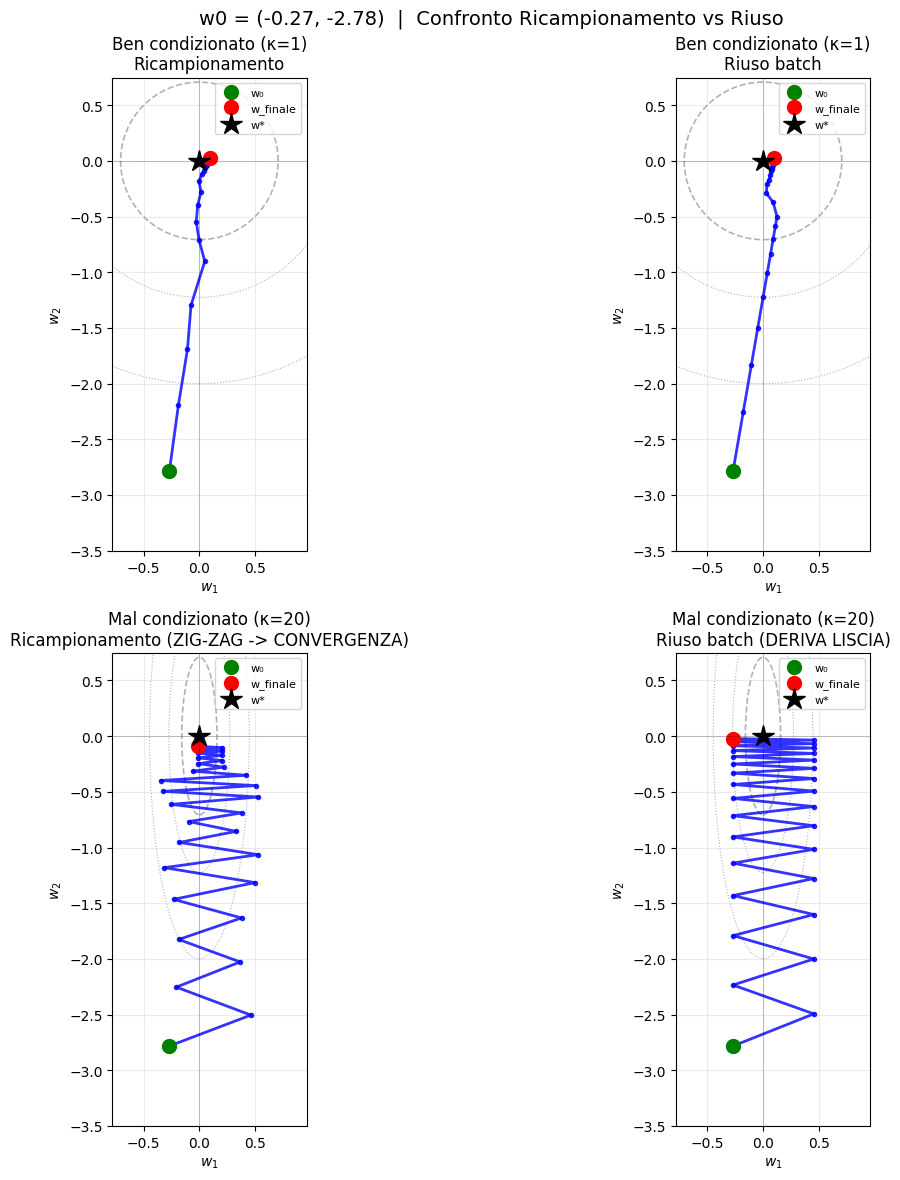
\includegraphics[width=\textwidth]{download.png}
\caption{Traiettorie di Dynamic GD con ricampionamento (colonna sinistra) e
riuso del batch (colonna destra), su problema ben condizionato ($\kappa=1$,
riga superiore) e mal condizionato ($\kappa=20$, riga inferiore). Punto
iniziale $w_0=(-0.27,-2.78)$; le curve di livello tratteggiate mostrano
$J(w)=\kappa w_1^2 + w_2^2$. I punti blu marcano le iterazioni in cui la
condizione CCV risulta violata.}
\label{fig:riuso_traiettorie}
\end{figure}

\subsubsection{Setup sperimentale}\label{app:riuso-setup}

Gli esperimenti usano gli stessi problemi, parametri e seed della
Sezione~\ref{sec:setup}: quattro preset quadratici ($\kappa \approx 1.1$,
$\kappa \approx 20$, $\kappa \approx 100$ e termine incrociato), $N = 200$
esempi sintetici, $w_0 = (2, -3)$, $\alpha = 0.1$, $\theta = 0.5$, $n_0 = 5$,
30 iterazioni, line search di Wolfe (Armijo per BB-CCV), seed 42. Per
ciascuno dei quattro algoritmi -- Dynamic GD, Newton-CG, Newton-CG~$L_1$ e
BB-CCV -- si confrontano la versione a ricampionamento (colonna \emph{base}) e
il riuso dello stesso mini-batch per $M$ iterazioni consecutive
($M \in \{\infty, 10, 5, 2\}$; la Tabella~\ref{tab:riuso_sintesi} estende la
sintesi a $M \in \{\infty, 10, 5, 3, 2, 1\}$).

Per i metodi di Newton la Hessiana è stimata sul sottoinsieme $H_k \subseteq
\mathcal{S}_k$ di dimensione $n_h = \min(\max(1, \lceil R n_k \rceil), N)$
(opzione \emph{Sottocampionamento Hessiana} dell'app, default \emph{Subset},
coerente con la Sezione~\ref{sec:setup}). Le colonne $M{=}\infty$, $M{=}10$,
$M{=}5$, $M{=}2$ delle tabelle dei metodi di Newton
(Tabelle~\ref{tab:riuso_bencond_ncg}--\ref{tab:riuso_offdiag_l1}) usano la
modalità \emph{Legato a $S_k$} (default): $H_k$ è ricampionata insieme a
$S_k$. L'ultima colonna ($M{=}10$, H ind. $M_H{=}\infty$) usa la modalità
\emph{Indipendente da $S_k$} con $M_H$ illimitato: a parità di riuso del batch
($M = 10$) l'Hessiana resta in uso finché la CCV è soddisfatta, senza seguire
il contatore del batch. Con $M = \infty$ le due modalità coincidono
(Sezione~\ref{app:riuso-descrizione}); la modalità indipendente è quindi
testata solo con batch finito.

Le righe in testa alle tabelle dei metodi di Newton
($M$, $M_H$, $H_k$) riportano, per ciascuna colonna, il riuso del
mini-batch, il riuso dell'Hessiana e la modalità (legata o indipendente
da $S_k$).

\subsubsection{Risultati numerici}\label{app:riuso-risultati}

Le Tabelle~\ref{tab:riuso_bencond_gd}--\ref{tab:riuso_offdiag_bb} riportano
l'errore $e_k = \|w_k - w^*\|_2$ iterazione per iterazione. Il quadro
emerso è coerente con l'analisi della Sezione~\ref{app:riuso-meccanismo}:

\begin{itemize}
\item Dynamic GD e BB-CCV si comportano in modo quasi identico.
  Su $\kappa \approx 1.1$ il riuso migliora sistematicamente (5 seed su 5
  con $M=\infty$ e $M=10$), con il vantaggio che emerge nella seconda metà
  delle iterazioni. Su $\kappa \approx 20$ il riuso illimitato peggiora;
  su $\kappa \approx 100$ il riuso torna ad aiutare.
\item Newton-CG è penalizzato quasi universalmente, con l'eccezione
  del problema con termine incrociato con $M=\infty$.
\item Newton-CG $L_1$ ha comportamento intermedio, senza una
  tendenza netta.
\item La modalità \emph{Indipendente da $S_k$} (colonna $M{=}10$, H ind.
  $M_H{=}\infty$) sposta il compromesso. Rispetto alla colonna $M{=}10$ legata
  (stessa politica di batch), tenere l'Hessiana oltre i ricampionamenti del
  batch migliora Newton-CG sul problema ben condizionato
  ($3.15\times10^{-1}$ contro $3.74\times10^{-1}$) e Newton-CG~$L_1$ sul
  termine incrociato ($2.50\times10^{-2}$ contro $3.94\times10^{-2}$), mentre
  peggiora Newton-CG sui problemi mal condizionati ($\kappa\approx20$:
  $1.15\times10^{0}$ contro $9.49\times10^{-1}$; $\kappa\approx100$:
  $1.16\times10^{0}$ contro $6.44\times10^{-1}$), dove la direzione resta più
  a lungo ancorata alla Hessiana del campione iniziale.
\end{itemize}

Vale la pena notare che le curve di errore con il riuso non sono monotone
rispetto alla base iterazione per iterazione: anche nei casi in cui l'errore
finale è migliore, ci sono fasi intermedie in cui è temporaneamente più alto,
perché la line search garantisce la discesa solo sulla loss del batch corrente,
non sulla funzione intera.

\subsubsection{Sintesi: quando il riuso aiuta e quando no}\label{app:riuso-sintesi}

La Tabella~\ref{tab:riuso_sintesi} riassume l'errore finale $e_{30}$ per tutti
i valori di $M$; la Tabella~\ref{tab:riuso_robustezza} riporta la robustezza
su cinque seed indipendenti.

\begin{itemize}
\item Il riuso aiuta quando il problema è ben condizionato: il minimo
  campionato è vicino a $w^*$ in tutte le direzioni, i passi coerenti riducono
  il rimbalzo attorno al minimo e l'iterato scende sotto il pavimento di
  rumore.
\item Il riuso non aiuta quando il problema è mal condizionato
  (deriva verso il minimo campionario, non rilevata dalla CCV) o si usano
  metodi del secondo ordine (Hessiana obsoleta).
\item La modalità \emph{Indipendente da $S_k$} con $M_H=\infty$ non cambia il
  quadro qualitativo: la colonna $M{=}10$, H ind. $M_H{=}\infty$ segue
  l'andamento della colonna $M{=}10$ legata, con lievi miglioramenti sui
  problemi ben condizionati e sul termine incrociato e un peggioramento
  confermato sui mal condizionati di Newton-CG. Il suo ruolo è quello di
  disaccoppiare la frequenza di ricampionamento dell'Hessiana da quella del
  batch: con $M=\infty$ la scelta diventa ininfluente, perché entrambe le
  modalità ricampionano solo alla violazione della CCV.
\end{itemize}

\paragraph{Osservazione sul costo computazionale.}
Il confronto è fatto a parità di iterazioni. Il riuso è già favorito dal
punto di vista del costo: Dynamic GD e BB-CCV non richiedono calcoli
aggiuntivi; Newton-CG nella versione base spende un campione fresco a ogni
iterazione solo per valutare la CCV. Il fatto che nonostante questo vantaggio
il riuso non sia sempre vincente rende i casi negativi ancora più significativi:
il problema è di qualità delle direzioni di discesa, non di costo.

% ====================================================================================================
% Tabelle E.1-E.16: errore a ogni iterazione (riuso del mini-batch)
% Generate da /tmp/gen_tabelle2.py - NON modificare a mano i valori.
% ====================================================================================================

% Tabella E.1 - quad_well, Dynamic GD
\begin{table}[H]
\centering
\footnotesize
\renewcommand{\arraystretch}{0.85}
\setlength{\tabcolsep}{4pt}
\caption{Errore $e_k=\|w_k-w_*\|_2$ a ogni iterazione $k$ sul problema quadratico ben condizionato ($\kappa\approx 1.1$), per \emph{Dynamic GD}: confronto tra la versione a ricampionamento (colonna \emph{base}) e il riuso dello stesso mini-batch per $M$ iterazioni consecutive ($M=\infty$: illimitato). Valori al seed 42, setup della Sezione~\ref{sec:setup}.}
\label{tab:riuso_bencond_gd}
\begin{tabular}{@{}rrrrrr@{}}
\toprule
$k$ & \emph{base} & $M{=}\infty$ & $M{=}10$ & $M{=}5$ & $M{=}2$\\
\midrule
0 & $1.4142\times10^{0}$ & $1.4142\times10^{0}$ & $1.4142\times10^{0}$ & $1.4142\times10^{0}$ & $1.4142\times10^{0}$\\
1 & $1.1516\times10^{0}$ & $1.1516\times10^{0}$ & $1.1516\times10^{0}$ & $1.1516\times10^{0}$ & $1.1516\times10^{0}$\\
2 & $9.5519\times10^{-1}$ & $9.3935\times10^{-1}$ & $9.3935\times10^{-1}$ & $9.3935\times10^{-1}$ & $9.3935\times10^{-1}$\\
3 & $7.8850\times10^{-1}$ & $7.6789\times10^{-1}$ & $7.6789\times10^{-1}$ & $7.6789\times10^{-1}$ & $7.8293\times10^{-1}$\\
4 & $6.7471\times10^{-1}$ & $6.2940\times10^{-1}$ & $6.2940\times10^{-1}$ & $6.2940\times10^{-1}$ & $6.5623\times10^{-1}$\\
5 & $5.5214\times10^{-1}$ & $5.1757\times10^{-1}$ & $5.1757\times10^{-1}$ & $5.1757\times10^{-1}$ & $5.4593\times10^{-1}$\\
6 & $4.3385\times10^{-1}$ & $4.2731\times10^{-1}$ & $4.2731\times10^{-1}$ & $4.4035\times10^{-1}$ & $4.5648\times10^{-1}$\\
7 & $3.8792\times10^{-1}$ & $3.5451\times10^{-1}$ & $3.5451\times10^{-1}$ & $3.7811\times10^{-1}$ & $4.0797\times10^{-1}$\\
8 & $3.5366\times10^{-1}$ & $2.9583\times10^{-1}$ & $2.9583\times10^{-1}$ & $3.2801\times10^{-1}$ & $3.7052\times10^{-1}$\\
9 & $3.0927\times10^{-1}$ & $2.4860\times10^{-1}$ & $2.4860\times10^{-1}$ & $2.8772\times10^{-1}$ & $3.1646\times10^{-1}$\\
10 & $2.5516\times10^{-1}$ & $2.1063\times10^{-1}$ & $2.1063\times10^{-1}$ & $2.4659\times10^{-1}$ & $2.7796\times10^{-1}$\\
11 & $2.3129\times10^{-1}$ & $1.7823\times10^{-1}$ & $1.7823\times10^{-1}$ & $2.4346\times10^{-1}$ & $2.3093\times10^{-1}$\\
12 & $2.1401\times10^{-1}$ & $1.5662\times10^{-1}$ & $1.5662\times10^{-1}$ & $2.2097\times10^{-1}$ & $1.9685\times10^{-1}$\\
13 & $2.0084\times10^{-1}$ & $1.4060\times10^{-1}$ & $1.4060\times10^{-1}$ & $2.0277\times10^{-1}$ & $1.8284\times10^{-1}$\\
14 & $1.8252\times10^{-1}$ & $1.3342\times10^{-1}$ & $1.3342\times10^{-1}$ & $1.8804\times10^{-1}$ & $1.6456\times10^{-1}$\\
15 & $1.6601\times10^{-1}$ & $1.2886\times10^{-1}$ & $1.2886\times10^{-1}$ & $1.7613\times10^{-1}$ & $1.5065\times10^{-1}$\\
16 & $1.6395\times10^{-1}$ & $1.3345\times10^{-1}$ & $1.3345\times10^{-1}$ & $1.6649\times10^{-1}$ & $1.4519\times10^{-1}$\\
17 & $1.5471\times10^{-1}$ & $1.3005\times10^{-1}$ & $1.3005\times10^{-1}$ & $1.5698\times10^{-1}$ & $1.3899\times10^{-1}$\\
18 & $1.4730\times10^{-1}$ & $1.2735\times10^{-1}$ & $1.2735\times10^{-1}$ & $1.4930\times10^{-1}$ & $1.3420\times10^{-1}$\\
19 & $1.4134\times10^{-1}$ & $1.2521\times10^{-1}$ & $1.2521\times10^{-1}$ & $1.4302\times10^{-1}$ & $1.3048\times10^{-1}$\\
20 & $1.3654\times10^{-1}$ & $1.2350\times10^{-1}$ & $1.2350\times10^{-1}$ & $1.3796\times10^{-1}$ & $1.2758\times10^{-1}$\\
21 & $1.3268\times10^{-1}$ & $1.2214\times10^{-1}$ & $1.2214\times10^{-1}$ & $1.3388\times10^{-1}$ & $1.2531\times10^{-1}$\\
22 & $1.2957\times10^{-1}$ & $1.2105\times10^{-1}$ & $1.2105\times10^{-1}$ & $1.3058\times10^{-1}$ & $1.2353\times10^{-1}$\\
23 & $1.2707\times10^{-1}$ & $1.2017\times10^{-1}$ & $1.2017\times10^{-1}$ & $1.2791\times10^{-1}$ & $1.2212\times10^{-1}$\\
24 & $1.2505\times10^{-1}$ & $1.1948\times10^{-1}$ & $1.1948\times10^{-1}$ & $1.2576\times10^{-1}$ & $1.2101\times10^{-1}$\\
25 & $1.2342\times10^{-1}$ & $1.1891\times10^{-1}$ & $1.1891\times10^{-1}$ & $1.2402\times10^{-1}$ & $1.2012\times10^{-1}$\\
26 & $1.2211\times10^{-1}$ & $1.1846\times10^{-1}$ & $1.1846\times10^{-1}$ & $1.2261\times10^{-1}$ & $1.1942\times10^{-1}$\\
27 & $1.2105\times10^{-1}$ & $1.1810\times10^{-1}$ & $1.1810\times10^{-1}$ & $1.2147\times10^{-1}$ & $1.1886\times10^{-1}$\\
28 & $1.2020\times10^{-1}$ & $1.1781\times10^{-1}$ & $1.1781\times10^{-1}$ & $1.2055\times10^{-1}$ & $1.1842\times10^{-1}$\\
29 & $1.1951\times10^{-1}$ & $1.1758\times10^{-1}$ & $1.1758\times10^{-1}$ & $1.1980\times10^{-1}$ & $1.1806\times10^{-1}$\\
30 & $1.1895\times10^{-1}$ & $1.1739\times10^{-1}$ & $1.1739\times10^{-1}$ & $1.1920\times10^{-1}$ & $1.1777\times10^{-1}$\\
\bottomrule
\end{tabular}
\end{table}

% Tabella E.2 - quad_well, Newton-CG
\begin{table}[H]
\centering
\footnotesize
\renewcommand{\arraystretch}{0.85}
\setlength{\tabcolsep}{2pt}
\caption{Errore $e_k=\|w_k-w_*\|_2$ a ogni iterazione $k$ sul problema quadratico ben condizionato ($\kappa\approx 1.1$), per \emph{Newton-CG}: confronto tra la versione a ricampionamento (colonna \emph{base}) e il riuso dello stesso mini-batch per $M$ iterazioni consecutive. Le righe in testa riportano, per ciascuna colonna, il riuso del batch $M$, il riuso dell'Hessiana $M_H$ e la modalità ($H_k$ legata o indipendente da $S_k$). Valori al seed 42, setup della Sezione~\ref{sec:setup}.}
\label{tab:riuso_bencond_ncg}
\begin{tabular}{@{}rrrrrrr@{}}
\toprule
$k$ & \emph{base} & $\infty$ & $10$ & $5$ & $2$ & H ind.\\
$M$ & $1$ & $\infty$ & $10$ & $5$ & $2$ & $10$\\
$M_H$ & $1$ & $\infty$ & $10$ & $5$ & $2$ & $\infty$\\
$H_k$ & legata & legata & legata & legata & legata & indipendente\\
\midrule
0 & $1.4142\times10^{0}$ & $1.4142\times10^{0}$ & $1.4142\times10^{0}$ & $1.4142\times10^{0}$ & $1.4142\times10^{0}$ & $1.4142\times10^{0}$\\
1 & $1.2758\times10^{0}$ & $1.2758\times10^{0}$ & $1.2758\times10^{0}$ & $1.2758\times10^{0}$ & $1.2758\times10^{0}$ & $1.2758\times10^{0}$\\
2 & $1.2758\times10^{0}$ & $1.1513\times10^{0}$ & $1.1513\times10^{0}$ & $1.1513\times10^{0}$ & $1.1513\times10^{0}$ & $1.1513\times10^{0}$\\
3 & $1.1736\times10^{0}$ & $1.0395\times10^{0}$ & $1.0395\times10^{0}$ & $1.0395\times10^{0}$ & $1.0614\times10^{0}$ & $1.0395\times10^{0}$\\
4 & $1.1736\times10^{0}$ & $9.3896\times10^{-1}$ & $9.3896\times10^{-1}$ & $9.3896\times10^{-1}$ & $9.8050\times10^{-1}$ & $9.3896\times10^{-1}$\\
5 & $1.1736\times10^{0}$ & $8.4861\times10^{-1}$ & $8.4861\times10^{-1}$ & $8.4861\times10^{-1}$ & $9.8050\times10^{-1}$ & $8.4861\times10^{-1}$\\
6 & $1.1736\times10^{0}$ & $7.6741\times10^{-1}$ & $7.6741\times10^{-1}$ & $7.8919\times10^{-1}$ & $9.8050\times10^{-1}$ & $7.6741\times10^{-1}$\\
7 & $1.0613\times10^{0}$ & $6.9443\times10^{-1}$ & $6.9443\times10^{-1}$ & $7.3584\times10^{-1}$ & $9.8050\times10^{-1}$ & $6.9443\times10^{-1}$\\
8 & $9.7253\times10^{-1}$ & $6.2886\times10^{-1}$ & $6.2886\times10^{-1}$ & $6.8796\times10^{-1}$ & $9.8050\times10^{-1}$ & $6.2886\times10^{-1}$\\
9 & $8.7008\times10^{-1}$ & $5.6994\times10^{-1}$ & $5.6994\times10^{-1}$ & $6.4498\times10^{-1}$ & $8.9503\times10^{-1}$ & $5.6994\times10^{-1}$\\
10 & $7.9049\times10^{-1}$ & $5.1700\times10^{-1}$ & $5.1700\times10^{-1}$ & $6.0643\times10^{-1}$ & $8.1845\times10^{-1}$ & $5.1700\times10^{-1}$\\
11 & $7.9049\times10^{-1}$ & $4.6944\times10^{-1}$ & $4.9121\times10^{-1}$ & $6.0643\times10^{-1}$ & $8.1845\times10^{-1}$ & $5.1700\times10^{-1}$\\
12 & $7.1398\times10^{-1}$ & $4.2673\times10^{-1}$ & $4.9121\times10^{-1}$ & $6.0643\times10^{-1}$ & $8.1845\times10^{-1}$ & $4.8916\times10^{-1}$\\
13 & $7.1398\times10^{-1}$ & $3.8836\times10^{-1}$ & $4.9121\times10^{-1}$ & $6.0643\times10^{-1}$ & $7.5191\times10^{-1}$ & $4.6429\times10^{-1}$\\
14 & $6.6137\times10^{-1}$ & $3.5392\times10^{-1}$ & $4.9121\times10^{-1}$ & $6.0643\times10^{-1}$ & $6.9207\times10^{-1}$ & $4.4208\times10^{-1}$\\
15 & $6.6137\times10^{-1}$ & $3.2300\times10^{-1}$ & $4.9121\times10^{-1}$ & $6.0643\times10^{-1}$ & $6.1429\times10^{-1}$ & $4.2226\times10^{-1}$\\
16 & $6.0964\times10^{-1}$ & $2.9526\times10^{-1}$ & $4.9121\times10^{-1}$ & $6.0643\times10^{-1}$ & $5.4461\times10^{-1}$ & $4.0457\times10^{-1}$\\
17 & $5.5345\times10^{-1}$ & $2.7036\times10^{-1}$ & $4.9121\times10^{-1}$ & $6.0643\times10^{-1}$ & $5.4461\times10^{-1}$ & $3.8878\times10^{-1}$\\
18 & $5.5345\times10^{-1}$ & $2.4804\times10^{-1}$ & $4.9121\times10^{-1}$ & $6.0643\times10^{-1}$ & $5.4461\times10^{-1}$ & $3.7284\times10^{-1}$\\
19 & $5.5345\times10^{-1}$ & $2.2803\times10^{-1}$ & $4.9121\times10^{-1}$ & $6.0643\times10^{-1}$ & $5.0538\times10^{-1}$ & $3.7284\times10^{-1}$\\
20 & $5.1627\times10^{-1}$ & $2.2230\times10^{-1}$ & $4.9121\times10^{-1}$ & $6.0643\times10^{-1}$ & $4.5035\times10^{-1}$ & $3.7284\times10^{-1}$\\
21 & $4.6784\times10^{-1}$ & $2.2230\times10^{-1}$ & $4.9121\times10^{-1}$ & $5.5923\times10^{-1}$ & $4.0161\times10^{-1}$ & $3.7284\times10^{-1}$\\
22 & $4.3254\times10^{-1}$ & $2.2230\times10^{-1}$ & $4.6205\times10^{-1}$ & $5.1703\times10^{-1}$ & $4.0161\times10^{-1}$ & $3.7284\times10^{-1}$\\
23 & $4.3254\times10^{-1}$ & $2.2230\times10^{-1}$ & $4.3604\times10^{-1}$ & $4.7931\times10^{-1}$ & $4.0161\times10^{-1}$ & $3.7284\times10^{-1}$\\
24 & $4.3254\times10^{-1}$ & $2.2230\times10^{-1}$ & $4.1284\times10^{-1}$ & $4.4561\times10^{-1}$ & $4.0161\times10^{-1}$ & $3.7284\times10^{-1}$\\
25 & $4.3254\times10^{-1}$ & $2.2230\times10^{-1}$ & $3.9215\times10^{-1}$ & $4.1553\times10^{-1}$ & $3.7003\times10^{-1}$ & $3.7284\times10^{-1}$\\
26 & $4.3254\times10^{-1}$ & $2.2230\times10^{-1}$ & $3.7373\times10^{-1}$ & $4.1553\times10^{-1}$ & $3.4184\times10^{-1}$ & $3.7284\times10^{-1}$\\
27 & $4.0264\times10^{-1}$ & $2.2230\times10^{-1}$ & $3.7373\times10^{-1}$ & $4.1553\times10^{-1}$ & $3.2879\times10^{-1}$ & $3.7284\times10^{-1}$\\
28 & $4.0264\times10^{-1}$ & $2.2230\times10^{-1}$ & $3.7373\times10^{-1}$ & $4.1553\times10^{-1}$ & $3.0362\times10^{-1}$ & $3.7284\times10^{-1}$\\
29 & $4.0264\times10^{-1}$ & $2.2230\times10^{-1}$ & $3.7373\times10^{-1}$ & $4.1553\times10^{-1}$ & $2.8102\times10^{-1}$ & $3.4233\times10^{-1}$\\
30 & $4.0264\times10^{-1}$ & $2.2230\times10^{-1}$ & $3.7373\times10^{-1}$ & $4.1553\times10^{-1}$ & $2.6069\times10^{-1}$ & $3.1490\times10^{-1}$\\
\bottomrule
\end{tabular}
\end{table}

% Tabella E.3 - quad_well, Newton-CG $L_1$
\begin{table}[H]
\centering
\footnotesize
\renewcommand{\arraystretch}{0.85}
\setlength{\tabcolsep}{2pt}
\caption{Errore $e_k=\|w_k-w_*\|_2$ a ogni iterazione $k$ sul problema quadratico ben condizionato ($\kappa\approx 1.1$), per \emph{Newton-CG $L_1$}: confronto tra la versione a ricampionamento (colonna \emph{base}) e il riuso dello stesso mini-batch per $M$ iterazioni consecutive. Le righe in testa riportano, per ciascuna colonna, il riuso del batch $M$, il riuso dell'Hessiana $M_H$ e la modalità ($H_k$ legata o indipendente da $S_k$). Valori al seed 42, setup della Sezione~\ref{sec:setup}.}
\label{tab:riuso_bencond_l1}
\begin{tabular}{@{}rrrrrrr@{}}
\toprule
$k$ & \emph{base} & $\infty$ & $10$ & $5$ & $2$ & H ind.\\
$M$ & $1$ & $\infty$ & $10$ & $5$ & $2$ & $10$\\
$M_H$ & $1$ & $\infty$ & $10$ & $5$ & $2$ & $\infty$\\
$H_k$ & legata & legata & legata & legata & legata & indipendente\\
\midrule
0 & $1.4142\times10^{0}$ & $1.4142\times10^{0}$ & $1.4142\times10^{0}$ & $1.4142\times10^{0}$ & $1.4142\times10^{0}$ & $1.4142\times10^{0}$\\
1 & $1.2683\times10^{0}$ & $1.2683\times10^{0}$ & $1.2683\times10^{0}$ & $1.2683\times10^{0}$ & $1.2683\times10^{0}$ & $1.2683\times10^{0}$\\
2 & $1.1466\times10^{0}$ & $1.1372\times10^{0}$ & $1.1372\times10^{0}$ & $1.1372\times10^{0}$ & $1.1372\times10^{0}$ & $1.1372\times10^{0}$\\
3 & $1.0501\times10^{0}$ & $1.0194\times10^{0}$ & $1.0194\times10^{0}$ & $1.0194\times10^{0}$ & $1.0413\times10^{0}$ & $1.0194\times10^{0}$\\
4 & $9.5532\times10^{-1}$ & $9.1344\times10^{-1}$ & $9.1344\times10^{-1}$ & $9.1344\times10^{-1}$ & $9.5508\times10^{-1}$ & $9.1344\times10^{-1}$\\
5 & $8.4970\times10^{-1}$ & $8.1824\times10^{-1}$ & $8.1824\times10^{-1}$ & $8.1824\times10^{-1}$ & $8.6356\times10^{-1}$ & $8.1824\times10^{-1}$\\
6 & $7.7334\times10^{-1}$ & $7.3268\times10^{-1}$ & $7.3268\times10^{-1}$ & $7.5455\times10^{-1}$ & $7.8120\times10^{-1}$ & $7.3268\times10^{-1}$\\
7 & $6.9434\times10^{-1}$ & $6.5580\times10^{-1}$ & $6.5580\times10^{-1}$ & $6.9738\times10^{-1}$ & $7.1613\times10^{-1}$ & $6.5580\times10^{-1}$\\
8 & $6.3606\times10^{-1}$ & $5.8671\times10^{-1}$ & $5.8671\times10^{-1}$ & $6.4606\times10^{-1}$ & $6.5742\times10^{-1}$ & $5.8671\times10^{-1}$\\
9 & $5.6016\times10^{-1}$ & $5.2465\times10^{-1}$ & $5.2465\times10^{-1}$ & $6.0002\times10^{-1}$ & $5.9800\times10^{-1}$ & $5.2465\times10^{-1}$\\
10 & $5.0464\times10^{-1}$ & $4.6889\times10^{-1}$ & $4.6889\times10^{-1}$ & $5.5871\times10^{-1}$ & $5.4482\times10^{-1}$ & $4.6889\times10^{-1}$\\
11 & $4.5898\times10^{-1}$ & $4.1881\times10^{-1}$ & $4.4080\times10^{-1}$ & $5.1057\times10^{-1}$ & $4.7301\times10^{-1}$ & $4.4103\times10^{-1}$\\
12 & $4.2560\times10^{-1}$ & $3.7385\times10^{-1}$ & $3.9703\times10^{-1}$ & $4.6741\times10^{-1}$ & $4.0866\times10^{-1}$ & $4.0947\times10^{-1}$\\
13 & $3.9782\times10^{-1}$ & $3.3349\times10^{-1}$ & $3.5791\times10^{-1}$ & $4.2876\times10^{-1}$ & $3.7575\times10^{-1}$ & $3.8129\times10^{-1}$\\
14 & $3.5221\times10^{-1}$ & $2.9727\times10^{-1}$ & $3.2301\times10^{-1}$ & $3.9418\times10^{-1}$ & $3.4617\times10^{-1}$ & $3.5615\times10^{-1}$\\
15 & $3.1656\times10^{-1}$ & $2.6479\times10^{-1}$ & $2.9192\times10^{-1}$ & $3.6330\times10^{-1}$ & $3.0862\times10^{-1}$ & $3.3373\times10^{-1}$\\
16 & $2.8037\times10^{-1}$ & $2.3569\times10^{-1}$ & $2.6427\times10^{-1}$ & $3.3812\times10^{-1}$ & $2.7484\times10^{-1}$ & $3.1376\times10^{-1}$\\
17 & $2.5757\times10^{-1}$ & $2.2206\times10^{-1}$ & $2.3975\times10^{-1}$ & $3.1547\times10^{-1}$ & $2.5601\times10^{-1}$ & $2.9598\times10^{-1}$\\
18 & $2.3404\times10^{-1}$ & $2.0090\times10^{-1}$ & $2.1806\times10^{-1}$ & $2.9511\times10^{-1}$ & $2.3744\times10^{-1}$ & $2.6746\times10^{-1}$\\
19 & $2.1740\times10^{-1}$ & $1.8212\times10^{-1}$ & $1.9894\times10^{-1}$ & $2.6100\times10^{-1}$ & $2.1890\times10^{-1}$ & $2.4198\times10^{-1}$\\
20 & $2.0263\times10^{-1}$ & $1.6549\times10^{-1}$ & $1.7907\times10^{-1}$ & $2.3031\times10^{-1}$ & $2.0226\times10^{-1}$ & $2.1927\times10^{-1}$\\
21 & $1.8691\times10^{-1}$ & $1.5082\times10^{-1}$ & $1.6648\times10^{-1}$ & $2.0269\times10^{-1}$ & $1.8738\times10^{-1}$ & $1.9904\times10^{-1}$\\
22 & $1.7550\times10^{-1}$ & $1.3794\times10^{-1}$ & $1.5297\times10^{-1}$ & $1.7783\times10^{-1}$ & $1.7413\times10^{-1}$ & $1.8107\times10^{-1}$\\
23 & $1.6345\times10^{-1}$ & $1.2668\times10^{-1}$ & $1.4368\times10^{-1}$ & $1.5830\times10^{-1}$ & $1.5548\times10^{-1}$ & $1.6234\times10^{-1}$\\
24 & $1.5147\times10^{-1}$ & $1.1689\times10^{-1}$ & $1.3370\times10^{-1}$ & $1.5337\times10^{-1}$ & $1.3882\times10^{-1}$ & $1.4573\times10^{-1}$\\
25 & $1.4067\times10^{-1}$ & $1.0814\times10^{-1}$ & $1.2477\times10^{-1}$ & $1.4207\times10^{-1}$ & $1.2628\times10^{-1}$ & $1.3203\times10^{-1}$\\
26 & $1.3109\times10^{-1}$ & $1.0071\times10^{-1}$ & $1.1675\times10^{-1}$ & $1.3046\times10^{-1}$ & $1.2219\times10^{-1}$ & $1.2482\times10^{-1}$\\
27 & $1.2247\times10^{-1}$ & $9.5081\times10^{-2}$ & $1.0961\times10^{-1}$ & $1.2096\times10^{-1}$ & $1.1189\times10^{-1}$ & $1.1695\times10^{-1}$\\
28 & $1.1474\times10^{-1}$ & $9.0108\times10^{-2}$ & $1.0321\times10^{-1}$ & $1.1322\times10^{-1}$ & $1.0527\times10^{-1}$ & $1.0981\times10^{-1}$\\
29 & $1.0786\times10^{-1}$ & $8.5687\times10^{-2}$ & $9.7485\times10^{-2}$ & $1.0627\times10^{-1}$ & $9.9372\times10^{-2}$ & $1.0343\times10^{-1}$\\
30 & $1.0167\times10^{-1}$ & $8.1750\times10^{-2}$ & $9.2407\times10^{-2}$ & $1.0010\times10^{-1}$ & $9.4078\times10^{-2}$ & $9.7785\times10^{-2}$\\
\bottomrule
\end{tabular}
\end{table}

% Tabella E.4 - quad_well, BB-CCV
\begin{table}[H]
\centering
\footnotesize
\renewcommand{\arraystretch}{0.85}
\setlength{\tabcolsep}{4pt}
\caption{Errore $e_k=\|w_k-w_*\|_2$ a ogni iterazione $k$ sul problema quadratico ben condizionato ($\kappa\approx 1.1$), per \emph{BB-CCV}: confronto tra la versione a ricampionamento (colonna \emph{base}) e il riuso dello stesso mini-batch per $M$ iterazioni consecutive ($M=\infty$: illimitato). Valori al seed 42, setup della Sezione~\ref{sec:setup}.}
\label{tab:riuso_bencond_bb}
\begin{tabular}{@{}rrrrrr@{}}
\toprule
$k$ & \emph{base} & $M{=}\infty$ & $M{=}10$ & $M{=}5$ & $M{=}2$\\
\midrule
0 & $1.4142\times10^{0}$ & $1.4142\times10^{0}$ & $1.4142\times10^{0}$ & $1.4142\times10^{0}$ & $1.4142\times10^{0}$\\
1 & $1.1516\times10^{0}$ & $1.1516\times10^{0}$ & $1.1516\times10^{0}$ & $1.1516\times10^{0}$ & $1.1516\times10^{0}$\\
2 & $9.5519\times10^{-1}$ & $9.3935\times10^{-1}$ & $9.3935\times10^{-1}$ & $9.3935\times10^{-1}$ & $9.3935\times10^{-1}$\\
3 & $7.8850\times10^{-1}$ & $7.6789\times10^{-1}$ & $7.6789\times10^{-1}$ & $7.6789\times10^{-1}$ & $7.8293\times10^{-1}$\\
4 & $6.7471\times10^{-1}$ & $6.2940\times10^{-1}$ & $6.2940\times10^{-1}$ & $6.2940\times10^{-1}$ & $6.5623\times10^{-1}$\\
5 & $5.5214\times10^{-1}$ & $5.1757\times10^{-1}$ & $5.1757\times10^{-1}$ & $5.1757\times10^{-1}$ & $5.4593\times10^{-1}$\\
6 & $4.3385\times10^{-1}$ & $4.2731\times10^{-1}$ & $4.2731\times10^{-1}$ & $4.4035\times10^{-1}$ & $4.5648\times10^{-1}$\\
7 & $3.8792\times10^{-1}$ & $3.5451\times10^{-1}$ & $3.5451\times10^{-1}$ & $3.7811\times10^{-1}$ & $4.0797\times10^{-1}$\\
8 & $3.5366\times10^{-1}$ & $2.9583\times10^{-1}$ & $2.9583\times10^{-1}$ & $3.2801\times10^{-1}$ & $3.7052\times10^{-1}$\\
9 & $3.0927\times10^{-1}$ & $2.4860\times10^{-1}$ & $2.4860\times10^{-1}$ & $2.8772\times10^{-1}$ & $3.1646\times10^{-1}$\\
10 & $2.5516\times10^{-1}$ & $2.1063\times10^{-1}$ & $2.1063\times10^{-1}$ & $2.4659\times10^{-1}$ & $2.7796\times10^{-1}$\\
11 & $2.3129\times10^{-1}$ & $1.7823\times10^{-1}$ & $1.7823\times10^{-1}$ & $2.4346\times10^{-1}$ & $2.3093\times10^{-1}$\\
12 & $2.1401\times10^{-1}$ & $1.5662\times10^{-1}$ & $1.5662\times10^{-1}$ & $2.2097\times10^{-1}$ & $1.9685\times10^{-1}$\\
13 & $2.0084\times10^{-1}$ & $1.4060\times10^{-1}$ & $1.4060\times10^{-1}$ & $2.0277\times10^{-1}$ & $1.8284\times10^{-1}$\\
14 & $1.8252\times10^{-1}$ & $1.3342\times10^{-1}$ & $1.3342\times10^{-1}$ & $1.8804\times10^{-1}$ & $1.6456\times10^{-1}$\\
15 & $1.6601\times10^{-1}$ & $1.2886\times10^{-1}$ & $1.2886\times10^{-1}$ & $1.7613\times10^{-1}$ & $1.5065\times10^{-1}$\\
16 & $1.6395\times10^{-1}$ & $1.3345\times10^{-1}$ & $1.3345\times10^{-1}$ & $1.6649\times10^{-1}$ & $1.4519\times10^{-1}$\\
17 & $1.5471\times10^{-1}$ & $1.3005\times10^{-1}$ & $1.3005\times10^{-1}$ & $1.5698\times10^{-1}$ & $1.3899\times10^{-1}$\\
18 & $1.4730\times10^{-1}$ & $1.2735\times10^{-1}$ & $1.2735\times10^{-1}$ & $1.4930\times10^{-1}$ & $1.3420\times10^{-1}$\\
19 & $1.4134\times10^{-1}$ & $1.2521\times10^{-1}$ & $1.2521\times10^{-1}$ & $1.4302\times10^{-1}$ & $1.3048\times10^{-1}$\\
20 & $1.3654\times10^{-1}$ & $1.2350\times10^{-1}$ & $1.2350\times10^{-1}$ & $1.3796\times10^{-1}$ & $1.2758\times10^{-1}$\\
21 & $1.3268\times10^{-1}$ & $1.2214\times10^{-1}$ & $1.2214\times10^{-1}$ & $1.3388\times10^{-1}$ & $1.2531\times10^{-1}$\\
22 & $1.2957\times10^{-1}$ & $1.2105\times10^{-1}$ & $1.2105\times10^{-1}$ & $1.3058\times10^{-1}$ & $1.2353\times10^{-1}$\\
23 & $1.2707\times10^{-1}$ & $1.2017\times10^{-1}$ & $1.2017\times10^{-1}$ & $1.2791\times10^{-1}$ & $1.2212\times10^{-1}$\\
24 & $1.2505\times10^{-1}$ & $1.1948\times10^{-1}$ & $1.1948\times10^{-1}$ & $1.2576\times10^{-1}$ & $1.2101\times10^{-1}$\\
25 & $1.2342\times10^{-1}$ & $1.1891\times10^{-1}$ & $1.1891\times10^{-1}$ & $1.2402\times10^{-1}$ & $1.2012\times10^{-1}$\\
26 & $1.2211\times10^{-1}$ & $1.1846\times10^{-1}$ & $1.1846\times10^{-1}$ & $1.2261\times10^{-1}$ & $1.1942\times10^{-1}$\\
27 & $1.2105\times10^{-1}$ & $1.1810\times10^{-1}$ & $1.1810\times10^{-1}$ & $1.2147\times10^{-1}$ & $1.1886\times10^{-1}$\\
28 & $1.2020\times10^{-1}$ & $1.1781\times10^{-1}$ & $1.1781\times10^{-1}$ & $1.2055\times10^{-1}$ & $1.1842\times10^{-1}$\\
29 & $1.1951\times10^{-1}$ & $1.1758\times10^{-1}$ & $1.1758\times10^{-1}$ & $1.1980\times10^{-1}$ & $1.1806\times10^{-1}$\\
30 & $1.1895\times10^{-1}$ & $1.1739\times10^{-1}$ & $1.1739\times10^{-1}$ & $1.1920\times10^{-1}$ & $1.1777\times10^{-1}$\\
\bottomrule
\end{tabular}
\end{table}


% Tabella E.5 - quad_ill, Dynamic GD
\begin{table}[H]
\centering
\footnotesize
\renewcommand{\arraystretch}{0.85}
\setlength{\tabcolsep}{4pt}
\caption{Errore $e_k=\|w_k-w_*\|_2$ a ogni iterazione $k$ sul problema quadratico mal condizionato ($\kappa\approx 20$), per \emph{Dynamic GD}: confronto tra la versione a ricampionamento (colonna \emph{base}) e il riuso dello stesso mini-batch per $M$ iterazioni consecutive ($M=\infty$: illimitato). Valori al seed 42, setup della Sezione~\ref{sec:setup}.}
\label{tab:riuso_malcond_gd}
\begin{tabular}{@{}rrrrrr@{}}
\toprule
$k$ & \emph{base} & $M{=}\infty$ & $M{=}10$ & $M{=}5$ & $M{=}2$\\
\midrule
0 & $1.4142\times10^{0}$ & $1.4142\times10^{0}$ & $1.4142\times10^{0}$ & $1.4142\times10^{0}$ & $1.4142\times10^{0}$\\
1 & $1.2185\times10^{0}$ & $1.2185\times10^{0}$ & $1.2185\times10^{0}$ & $1.2185\times10^{0}$ & $1.2185\times10^{0}$\\
2 & $1.2440\times10^{0}$ & $1.2895\times10^{0}$ & $1.2895\times10^{0}$ & $1.2895\times10^{0}$ & $1.2895\times10^{0}$\\
3 & $1.3338\times10^{0}$ & $1.1003\times10^{0}$ & $1.1003\times10^{0}$ & $1.1003\times10^{0}$ & $1.1459\times10^{0}$\\
4 & $1.3196\times10^{0}$ & $1.2001\times10^{0}$ & $1.2001\times10^{0}$ & $1.2001\times10^{0}$ & $1.2007\times10^{0}$\\
5 & $1.1515\times10^{0}$ & $1.0149\times10^{0}$ & $1.0149\times10^{0}$ & $1.0149\times10^{0}$ & $1.3173\times10^{0}$\\
6 & $1.3192\times10^{0}$ & $1.1372\times10^{0}$ & $1.1372\times10^{0}$ & $1.0853\times10^{0}$ & $1.1370\times10^{0}$\\
7 & $1.3119\times10^{0}$ & $9.5415\times10^{-1}$ & $9.5415\times10^{-1}$ & $9.5470\times10^{-1}$ & $1.0904\times10^{0}$\\
8 & $1.1849\times10^{0}$ & $1.0936\times10^{0}$ & $1.0936\times10^{0}$ & $1.0399\times10^{0}$ & $1.0950\times10^{0}$\\
9 & $1.1914\times10^{0}$ & $9.1173\times10^{-1}$ & $9.1173\times10^{-1}$ & $9.1259\times10^{-1}$ & $9.3482\times10^{-1}$\\
10 & $1.3429\times10^{0}$ & $1.0637\times10^{0}$ & $1.0637\times10^{0}$ & $1.0086\times10^{0}$ & $1.0622\times10^{0}$\\
11 & $1.3922\times10^{0}$ & $8.8246\times10^{-1}$ & $9.3840\times10^{-1}$ & $1.1610\times10^{0}$ & $8.4194\times10^{-1}$\\
12 & $2.9524\times10^{-1}$ & $1.0434\times10^{0}$ & $1.0437\times10^{0}$ & $9.8645\times10^{-1}$ & $1.0399\times10^{0}$\\
13 & $2.6608\times10^{-1}$ & $8.6245\times10^{-1}$ & $9.1986\times10^{-1}$ & $1.1455\times10^{0}$ & $1.0468\times10^{0}$\\
14 & $2.3965\times10^{-1}$ & $1.0296\times10^{0}$ & $1.0301\times10^{0}$ & $9.7151\times10^{-1}$ & $1.0255\times10^{0}$\\
15 & $2.1588\times10^{-1}$ & $8.4883\times10^{-1}$ & $9.0722\times10^{-1}$ & $1.1350\times10^{0}$ & $1.1311\times10^{0}$\\
16 & $1.9451\times10^{-1}$ & $1.0203\times10^{0}$ & $1.0209\times10^{0}$ & $2.1297\times10^{-1}$ & $1.0139\times10^{0}$\\
17 & $1.7531\times10^{-1}$ & $2.1374\times10^{-1}$ & $2.0559\times10^{-1}$ & $1.7879\times10^{-1}$ & $1.6351\times10^{-1}$\\
18 & $1.5805\times10^{-1}$ & $1.8311\times10^{-1}$ & $1.7350\times10^{-1}$ & $1.6101\times10^{-1}$ & $1.4840\times10^{-1}$\\
19 & $1.4254\times10^{-1}$ & $1.6945\times10^{-1}$ & $1.5836\times10^{-1}$ & $1.4502\times10^{-1}$ & $1.3362\times10^{-1}$\\
20 & $1.2862\times10^{-1}$ & $1.5752\times10^{-1}$ & $1.4495\times10^{-1}$ & $1.3065\times10^{-1}$ & $1.2033\times10^{-1}$\\
21 & $1.1613\times10^{-1}$ & $1.4715\times10^{-1}$ & $1.3311\times10^{-1}$ & $1.1772\times10^{-1}$ & $1.0838\times10^{-1}$\\
22 & $1.0492\times10^{-1}$ & $1.3818\times10^{-1}$ & $1.2267\times10^{-1}$ & $1.0611\times10^{-1}$ & $9.7628\times10^{-2}$\\
23 & $9.4880\times10^{-2}$ & $1.3047\times10^{-1}$ & $1.1352\times10^{-1}$ & $9.5672\times10^{-2}$ & $8.7964\times10^{-2}$\\
24 & $8.5890\times10^{-2}$ & $1.2387\times10^{-1}$ & $1.0552\times10^{-1}$ & $8.6298\times10^{-2}$ & $7.9276\times10^{-2}$\\
25 & $7.7851\times10^{-2}$ & $1.1825\times10^{-1}$ & $9.8576\times10^{-2}$ & $7.7882\times10^{-2}$ & $7.1470\times10^{-2}$\\
26 & $7.0673\times10^{-2}$ & $1.1350\times10^{-1}$ & $9.2566\times10^{-2}$ & $7.0330\times10^{-2}$ & $6.4457\times10^{-2}$\\
27 & $6.4273\times10^{-2}$ & $1.0950\times10^{-1}$ & $8.7395\times10^{-2}$ & $6.3559\times10^{-2}$ & $5.8160\times10^{-2}$\\
28 & $5.8579\times10^{-2}$ & $1.0614\times10^{-1}$ & $8.2971\times10^{-2}$ & $5.7493\times10^{-2}$ & $5.2508\times10^{-2}$\\
29 & $5.3525\times10^{-2}$ & $1.0335\times10^{-1}$ & $7.9206\times10^{-2}$ & $5.2064\times10^{-2}$ & $4.7440\times10^{-2}$\\
30 & $4.9050\times10^{-2}$ & $1.0103\times10^{-1}$ & $7.6020\times10^{-2}$ & $4.7211\times10^{-2}$ & $4.2898\times10^{-2}$\\
\bottomrule
\end{tabular}
\end{table}

% Tabella E.6 - quad_ill, Newton-CG
\begin{table}[H]
\centering
\footnotesize
\renewcommand{\arraystretch}{0.85}
\setlength{\tabcolsep}{2pt}
\caption{Errore $e_k=\|w_k-w_*\|_2$ a ogni iterazione $k$ sul problema quadratico mal condizionato ($\kappa\approx 20$), per \emph{Newton-CG}: confronto tra la versione a ricampionamento (colonna \emph{base}) e il riuso dello stesso mini-batch per $M$ iterazioni consecutive. Le righe in testa riportano, per ciascuna colonna, il riuso del batch $M$, il riuso dell'Hessiana $M_H$ e la modalità ($H_k$ legata o indipendente da $S_k$). Valori al seed 42, setup della Sezione~\ref{sec:setup}.}
\label{tab:riuso_malcond_ncg}
\begin{tabular}{@{}rrrrrrr@{}}
\toprule
$k$ & \emph{base} & $\infty$ & $10$ & $5$ & $2$ & H ind.\\
$M$ & $1$ & $\infty$ & $10$ & $5$ & $2$ & $10$\\
$M_H$ & $1$ & $\infty$ & $10$ & $5$ & $2$ & $\infty$\\
$H_k$ & legata & legata & legata & legata & legata & indipendente\\
\midrule
0 & $1.4142\times10^{0}$ & $1.4142\times10^{0}$ & $1.4142\times10^{0}$ & $1.4142\times10^{0}$ & $1.4142\times10^{0}$ & $1.4142\times10^{0}$\\
1 & $1.2807\times10^{0}$ & $1.2807\times10^{0}$ & $1.2807\times10^{0}$ & $1.2807\times10^{0}$ & $1.2807\times10^{0}$ & $1.2807\times10^{0}$\\
2 & $1.1526\times10^{0}$ & $1.2807\times10^{0}$ & $1.2807\times10^{0}$ & $1.2807\times10^{0}$ & $1.2807\times10^{0}$ & $1.2807\times10^{0}$\\
3 & $1.1526\times10^{0}$ & $1.2807\times10^{0}$ & $1.2807\times10^{0}$ & $1.2807\times10^{0}$ & $1.2807\times10^{0}$ & $1.2807\times10^{0}$\\
4 & $1.0395\times10^{0}$ & $1.2807\times10^{0}$ & $1.2807\times10^{0}$ & $1.2807\times10^{0}$ & $1.2807\times10^{0}$ & $1.2807\times10^{0}$\\
5 & $9.3153\times10^{-1}$ & $1.2807\times10^{0}$ & $1.2807\times10^{0}$ & $1.2807\times10^{0}$ & $1.1582\times10^{0}$ & $1.2807\times10^{0}$\\
6 & $9.3153\times10^{-1}$ & $1.2807\times10^{0}$ & $1.2807\times10^{0}$ & $1.2807\times10^{0}$ & $1.0482\times10^{0}$ & $1.2807\times10^{0}$\\
7 & $8.3758\times10^{-1}$ & $1.2807\times10^{0}$ & $1.2807\times10^{0}$ & $1.2807\times10^{0}$ & $9.4683\times10^{-1}$ & $1.2807\times10^{0}$\\
8 & $7.6704\times10^{-1}$ & $1.2807\times10^{0}$ & $1.2807\times10^{0}$ & $1.2807\times10^{0}$ & $9.4683\times10^{-1}$ & $1.2807\times10^{0}$\\
9 & $7.6704\times10^{-1}$ & $1.2807\times10^{0}$ & $1.2807\times10^{0}$ & $1.2807\times10^{0}$ & $8.4914\times10^{-1}$ & $1.2807\times10^{0}$\\
10 & $6.8050\times10^{-1}$ & $1.2807\times10^{0}$ & $1.2807\times10^{0}$ & $1.2807\times10^{0}$ & $8.4914\times10^{-1}$ & $1.2807\times10^{0}$\\
11 & $6.8050\times10^{-1}$ & $1.2807\times10^{0}$ & $1.2807\times10^{0}$ & $1.1582\times10^{0}$ & $7.6209\times10^{-1}$ & $1.2807\times10^{0}$\\
12 & $6.8050\times10^{-1}$ & $1.2807\times10^{0}$ & $1.2807\times10^{0}$ & $1.0482\times10^{0}$ & $6.8393\times10^{-1}$ & $1.2807\times10^{0}$\\
13 & $6.1045\times10^{-1}$ & $1.2807\times10^{0}$ & $1.2807\times10^{0}$ & $9.4933\times10^{-1}$ & $6.1644\times10^{-1}$ & $1.2807\times10^{0}$\\
14 & $6.1045\times10^{-1}$ & $1.2807\times10^{0}$ & $1.2807\times10^{0}$ & $9.4933\times10^{-1}$ & $5.5573\times10^{-1}$ & $1.2807\times10^{0}$\\
15 & $5.6100\times10^{-1}$ & $1.2807\times10^{0}$ & $1.2807\times10^{0}$ & $9.4933\times10^{-1}$ & $4.9972\times10^{-1}$ & $1.2807\times10^{0}$\\
16 & $5.0384\times10^{-1}$ & $1.2807\times10^{0}$ & $1.2807\times10^{0}$ & $8.5789\times10^{-1}$ & $4.4971\times10^{-1}$ & $1.2807\times10^{0}$\\
17 & $4.4985\times10^{-1}$ & $1.2807\times10^{0}$ & $1.2807\times10^{0}$ & $7.7559\times10^{-1}$ & $4.4971\times10^{-1}$ & $1.2807\times10^{0}$\\
18 & $4.0152\times10^{-1}$ & $1.2807\times10^{0}$ & $1.2807\times10^{0}$ & $7.0153\times10^{-1}$ & $4.4971\times10^{-1}$ & $1.2807\times10^{0}$\\
19 & $3.6498\times10^{-1}$ & $1.2807\times10^{0}$ & $1.2807\times10^{0}$ & $6.3487\times10^{-1}$ & $4.0617\times10^{-1}$ & $1.2807\times10^{0}$\\
20 & $3.6498\times10^{-1}$ & $1.2807\times10^{0}$ & $1.2807\times10^{0}$ & $6.3487\times10^{-1}$ & $4.0617\times10^{-1}$ & $1.2807\times10^{0}$\\
21 & $3.3037\times10^{-1}$ & $1.2807\times10^{0}$ & $1.1582\times10^{0}$ & $6.3487\times10^{-1}$ & $4.0617\times10^{-1}$ & $1.1526\times10^{0}$\\
22 & $2.9975\times10^{-1}$ & $1.2807\times10^{0}$ & $1.0482\times10^{0}$ & $6.3487\times10^{-1}$ & $4.0617\times10^{-1}$ & $1.1526\times10^{0}$\\
23 & $2.9975\times10^{-1}$ & $1.2807\times10^{0}$ & $9.4933\times10^{-1}$ & $6.3487\times10^{-1}$ & $4.0617\times10^{-1}$ & $1.1526\times10^{0}$\\
24 & $2.9975\times10^{-1}$ & $1.2807\times10^{0}$ & $9.4933\times10^{-1}$ & $6.3487\times10^{-1}$ & $4.0617\times10^{-1}$ & $1.1526\times10^{0}$\\
25 & $2.9975\times10^{-1}$ & $1.2807\times10^{0}$ & $9.4933\times10^{-1}$ & $6.3487\times10^{-1}$ & $4.0617\times10^{-1}$ & $1.1526\times10^{0}$\\
26 & $2.7805\times10^{-1}$ & $1.2807\times10^{0}$ & $9.4933\times10^{-1}$ & $5.6917\times10^{-1}$ & $4.0617\times10^{-1}$ & $1.1526\times10^{0}$\\
27 & $2.7805\times10^{-1}$ & $1.2807\times10^{0}$ & $9.4933\times10^{-1}$ & $5.1031\times10^{-1}$ & $4.0617\times10^{-1}$ & $1.1526\times10^{0}$\\
28 & $2.3463\times10^{-1}$ & $1.2807\times10^{0}$ & $9.4933\times10^{-1}$ & $4.5761\times10^{-1}$ & $4.0617\times10^{-1}$ & $1.1526\times10^{0}$\\
29 & $2.3463\times10^{-1}$ & $1.2807\times10^{0}$ & $9.4933\times10^{-1}$ & $4.1051\times10^{-1}$ & $4.0617\times10^{-1}$ & $1.1526\times10^{0}$\\
30 & $2.3463\times10^{-1}$ & $1.2807\times10^{0}$ & $9.4933\times10^{-1}$ & $4.1051\times10^{-1}$ & $4.0617\times10^{-1}$ & $1.1526\times10^{0}$\\
\bottomrule
\end{tabular}
\end{table}

% Tabella E.7 - quad_ill, Newton-CG $L_1$
\begin{table}[H]
\centering
\footnotesize
\renewcommand{\arraystretch}{0.85}
\setlength{\tabcolsep}{2pt}
\caption{Errore $e_k=\|w_k-w_*\|_2$ a ogni iterazione $k$ sul problema quadratico mal condizionato ($\kappa\approx 20$), per \emph{Newton-CG $L_1$}: confronto tra la versione a ricampionamento (colonna \emph{base}) e il riuso dello stesso mini-batch per $M$ iterazioni consecutive. Le righe in testa riportano, per ciascuna colonna, il riuso del batch $M$, il riuso dell'Hessiana $M_H$ e la modalità ($H_k$ legata o indipendente da $S_k$). Valori al seed 42, setup della Sezione~\ref{sec:setup}.}
\label{tab:riuso_malcond_l1}
\begin{tabular}{@{}rrrrrrr@{}}
\toprule
$k$ & \emph{base} & $\infty$ & $10$ & $5$ & $2$ & H ind.\\
$M$ & $1$ & $\infty$ & $10$ & $5$ & $2$ & $10$\\
$M_H$ & $1$ & $\infty$ & $10$ & $5$ & $2$ & $\infty$\\
$H_k$ & legata & legata & legata & legata & legata & indipendente\\
\midrule
0 & $1.4142\times10^{0}$ & $1.4142\times10^{0}$ & $1.4142\times10^{0}$ & $1.4142\times10^{0}$ & $1.4142\times10^{0}$ & $1.4142\times10^{0}$\\
1 & $1.3473\times10^{0}$ & $1.3473\times10^{0}$ & $1.3473\times10^{0}$ & $1.3473\times10^{0}$ & $1.3473\times10^{0}$ & $1.3473\times10^{0}$\\
2 & $1.2918\times10^{0}$ & $1.2892\times10^{0}$ & $1.2892\times10^{0}$ & $1.2892\times10^{0}$ & $1.2892\times10^{0}$ & $1.2892\times10^{0}$\\
3 & $1.2299\times10^{0}$ & $1.2389\times10^{0}$ & $1.2389\times10^{0}$ & $1.2389\times10^{0}$ & $1.2349\times10^{0}$ & $1.2389\times10^{0}$\\
4 & $1.1878\times10^{0}$ & $1.1954\times10^{0}$ & $1.1954\times10^{0}$ & $1.1954\times10^{0}$ & $1.1882\times10^{0}$ & $1.1954\times10^{0}$\\
5 & $1.1440\times10^{0}$ & $1.1577\times10^{0}$ & $1.1577\times10^{0}$ & $1.1577\times10^{0}$ & $1.1541\times10^{0}$ & $1.1577\times10^{0}$\\
6 & $1.1059\times10^{0}$ & $1.1250\times10^{0}$ & $1.1250\times10^{0}$ & $1.1217\times10^{0}$ & $1.1242\times10^{0}$ & $1.1250\times10^{0}$\\
7 & $1.0749\times10^{0}$ & $1.0966\times10^{0}$ & $1.0966\times10^{0}$ & $1.0907\times10^{0}$ & $1.0928\times10^{0}$ & $1.0966\times10^{0}$\\
8 & $1.0547\times10^{0}$ & $1.0719\times10^{0}$ & $1.0719\times10^{0}$ & $1.0641\times10^{0}$ & $1.0658\times10^{0}$ & $1.0719\times10^{0}$\\
9 & $1.0286\times10^{0}$ & $1.0502\times10^{0}$ & $1.0502\times10^{0}$ & $1.0411\times10^{0}$ & $1.0417\times10^{0}$ & $1.0502\times10^{0}$\\
10 & $1.0054\times10^{0}$ & $1.0312\times10^{0}$ & $1.0312\times10^{0}$ & $1.0212\times10^{0}$ & $1.0208\times10^{0}$ & $1.0312\times10^{0}$\\
11 & $9.9101\times10^{-1}$ & $1.0144\times10^{0}$ & $1.0121\times10^{0}$ & $1.0073\times10^{0}$ & $9.9952\times10^{-1}$ & $1.0121\times10^{0}$\\
12 & $9.7686\times10^{-1}$ & $9.9946\times10^{-1}$ & $9.9546\times10^{-1}$ & $9.9449\times10^{-1}$ & $9.8153\times10^{-1}$ & $9.9546\times10^{-1}$\\
13 & $9.6563\times10^{-1}$ & $9.8606\times10^{-1}$ & $9.8084\times10^{-1}$ & $9.7848\times10^{-1}$ & $9.6789\times10^{-1}$ & $9.8084\times10^{-1}$\\
14 & $9.5394\times10^{-1}$ & $9.7394\times10^{-1}$ & $9.6792\times10^{-1}$ & $9.6454\times10^{-1}$ & $9.5591\times10^{-1}$ & $9.6792\times10^{-1}$\\
15 & $9.4402\times10^{-1}$ & $9.6201\times10^{-1}$ & $9.5640\times10^{-1}$ & $9.5231\times10^{-1}$ & $9.4411\times10^{-1}$ & $9.5640\times10^{-1}$\\
16 & $9.3521\times10^{-1}$ & $9.5114\times10^{-1}$ & $9.4603\times10^{-1}$ & $9.4148\times10^{-1}$ & $9.3395\times10^{-1}$ & $9.4603\times10^{-1}$\\
17 & $9.2491\times10^{-1}$ & $9.4113\times10^{-1}$ & $9.3660\times10^{-1}$ & $9.3179\times10^{-1}$ & $9.2680\times10^{-1}$ & $9.3660\times10^{-1}$\\
18 & $8.2868\times10^{-1}$ & $9.3184\times10^{-1}$ & $9.2794\times10^{-1}$ & $9.2295\times10^{-1}$ & $9.1982\times10^{-1}$ & $9.2794\times10^{-1}$\\
19 & $8.2207\times10^{-1}$ & $9.2310\times10^{-1}$ & $9.1989\times10^{-1}$ & $9.1463\times10^{-1}$ & $9.1206\times10^{-1}$ & $9.1989\times10^{-1}$\\
20 & $8.1495\times10^{-1}$ & $9.1479\times10^{-1}$ & $9.1232\times10^{-1}$ & $9.0669\times10^{-1}$ & $8.1445\times10^{-1}$ & $9.1232\times10^{-1}$\\
21 & $8.0882\times10^{-1}$ & $9.0678\times10^{-1}$ & $8.1178\times10^{-1}$ & $8.9903\times10^{-1}$ & $8.0713\times10^{-1}$ & $8.0413\times10^{-1}$\\
22 & $8.0243\times10^{-1}$ & $8.9897\times10^{-1}$ & $8.0478\times10^{-1}$ & $8.9151\times10^{-1}$ & $8.0027\times10^{-1}$ & $7.9734\times10^{-1}$\\
23 & $7.1132\times10^{-1}$ & $8.9123\times10^{-1}$ & $7.9818\times10^{-1}$ & $7.9802\times10^{-1}$ & $7.9324\times10^{-1}$ & $7.9089\times10^{-1}$\\
24 & $6.3609\times10^{-1}$ & $8.8345\times10^{-1}$ & $7.9187\times10^{-1}$ & $7.9186\times10^{-1}$ & $6.9802\times10^{-1}$ & $7.8470\times10^{-1}$\\
25 & $6.3104\times10^{-1}$ & $8.7615\times10^{-1}$ & $7.8576\times10^{-1}$ & $7.1080\times10^{-1}$ & $6.2366\times10^{-1}$ & $7.7866\times10^{-1}$\\
26 & $6.2603\times10^{-1}$ & $8.6922\times10^{-1}$ & $7.7976\times10^{-1}$ & $6.3785\times10^{-1}$ & $5.5674\times10^{-1}$ & $7.7268\times10^{-1}$\\
27 & $5.5554\times10^{-1}$ & $8.6269\times10^{-1}$ & $7.7378\times10^{-1}$ & $6.3350\times10^{-1}$ & $4.9803\times10^{-1}$ & $6.9395\times10^{-1}$\\
28 & $5.5122\times10^{-1}$ & $7.7364\times10^{-1}$ & $6.9374\times10^{-1}$ & $6.2943\times10^{-1}$ & $4.9398\times10^{-1}$ & $6.8839\times10^{-1}$\\
29 & $4.9177\times10^{-1}$ & $7.6782\times10^{-1}$ & $6.2170\times10^{-1}$ & $6.2559\times10^{-1}$ & $4.8997\times10^{-1}$ & $6.8289\times10^{-1}$\\
30 & $4.8802\times10^{-1}$ & $7.6221\times10^{-1}$ & $5.5687\times10^{-1}$ & $6.2190\times10^{-1}$ & $4.3392\times10^{-1}$ & $6.0759\times10^{-1}$\\
\bottomrule
\end{tabular}
\end{table}

% Tabella E.8 - quad_ill, BB-CCV
\begin{table}[H]
\centering
\footnotesize
\renewcommand{\arraystretch}{0.85}
\setlength{\tabcolsep}{4pt}
\caption{Errore $e_k=\|w_k-w_*\|_2$ a ogni iterazione $k$ sul problema quadratico mal condizionato ($\kappa\approx 20$), per \emph{BB-CCV}: confronto tra la versione a ricampionamento (colonna \emph{base}) e il riuso dello stesso mini-batch per $M$ iterazioni consecutive ($M=\infty$: illimitato). Valori al seed 42, setup della Sezione~\ref{sec:setup}.}
\label{tab:riuso_malcond_bb}
\begin{tabular}{@{}rrrrrr@{}}
\toprule
$k$ & \emph{base} & $M{=}\infty$ & $M{=}10$ & $M{=}5$ & $M{=}2$\\
\midrule
0 & $1.4142\times10^{0}$ & $1.4142\times10^{0}$ & $1.4142\times10^{0}$ & $1.4142\times10^{0}$ & $1.4142\times10^{0}$\\
1 & $1.2185\times10^{0}$ & $1.2185\times10^{0}$ & $1.2185\times10^{0}$ & $1.2185\times10^{0}$ & $1.2185\times10^{0}$\\
2 & $1.2440\times10^{0}$ & $1.2895\times10^{0}$ & $1.2895\times10^{0}$ & $1.2895\times10^{0}$ & $1.2895\times10^{0}$\\
3 & $1.3338\times10^{0}$ & $1.1003\times10^{0}$ & $1.1003\times10^{0}$ & $1.1003\times10^{0}$ & $1.1459\times10^{0}$\\
4 & $1.3196\times10^{0}$ & $1.2001\times10^{0}$ & $1.2001\times10^{0}$ & $1.2001\times10^{0}$ & $1.2007\times10^{0}$\\
5 & $1.1515\times10^{0}$ & $1.0149\times10^{0}$ & $1.0149\times10^{0}$ & $1.0149\times10^{0}$ & $1.3173\times10^{0}$\\
6 & $1.3192\times10^{0}$ & $1.1372\times10^{0}$ & $1.1372\times10^{0}$ & $1.0853\times10^{0}$ & $1.1370\times10^{0}$\\
7 & $1.3119\times10^{0}$ & $9.5415\times10^{-1}$ & $9.5415\times10^{-1}$ & $9.5470\times10^{-1}$ & $1.0904\times10^{0}$\\
8 & $1.1849\times10^{0}$ & $1.0936\times10^{0}$ & $1.0936\times10^{0}$ & $1.0399\times10^{0}$ & $1.0950\times10^{0}$\\
9 & $1.1914\times10^{0}$ & $9.1173\times10^{-1}$ & $9.1173\times10^{-1}$ & $9.1259\times10^{-1}$ & $9.3482\times10^{-1}$\\
10 & $1.3429\times10^{0}$ & $1.0637\times10^{0}$ & $1.0637\times10^{0}$ & $1.0086\times10^{0}$ & $1.0622\times10^{0}$\\
11 & $1.3922\times10^{0}$ & $8.8246\times10^{-1}$ & $9.3840\times10^{-1}$ & $1.1610\times10^{0}$ & $8.4194\times10^{-1}$\\
12 & $2.9524\times10^{-1}$ & $1.0434\times10^{0}$ & $1.0437\times10^{0}$ & $9.8645\times10^{-1}$ & $1.0399\times10^{0}$\\
13 & $2.6608\times10^{-1}$ & $8.6245\times10^{-1}$ & $9.1986\times10^{-1}$ & $1.1455\times10^{0}$ & $1.0468\times10^{0}$\\
14 & $2.3965\times10^{-1}$ & $1.0296\times10^{0}$ & $1.0301\times10^{0}$ & $9.7151\times10^{-1}$ & $1.0255\times10^{0}$\\
15 & $2.1588\times10^{-1}$ & $8.4883\times10^{-1}$ & $9.0722\times10^{-1}$ & $1.1350\times10^{0}$ & $1.1311\times10^{0}$\\
16 & $1.9451\times10^{-1}$ & $1.0203\times10^{0}$ & $1.0209\times10^{0}$ & $2.1297\times10^{-1}$ & $1.0139\times10^{0}$\\
17 & $1.7531\times10^{-1}$ & $2.1374\times10^{-1}$ & $2.0559\times10^{-1}$ & $1.7879\times10^{-1}$ & $1.6351\times10^{-1}$\\
18 & $1.5805\times10^{-1}$ & $1.8311\times10^{-1}$ & $1.7350\times10^{-1}$ & $1.6101\times10^{-1}$ & $1.4840\times10^{-1}$\\
19 & $1.4254\times10^{-1}$ & $1.6945\times10^{-1}$ & $1.5836\times10^{-1}$ & $1.4502\times10^{-1}$ & $1.3362\times10^{-1}$\\
20 & $1.2862\times10^{-1}$ & $1.5752\times10^{-1}$ & $1.4495\times10^{-1}$ & $1.3065\times10^{-1}$ & $1.2033\times10^{-1}$\\
21 & $1.1613\times10^{-1}$ & $1.4715\times10^{-1}$ & $1.3311\times10^{-1}$ & $1.1772\times10^{-1}$ & $1.0838\times10^{-1}$\\
22 & $1.0492\times10^{-1}$ & $1.3818\times10^{-1}$ & $1.2267\times10^{-1}$ & $1.0611\times10^{-1}$ & $9.7628\times10^{-2}$\\
23 & $9.4880\times10^{-2}$ & $1.3047\times10^{-1}$ & $1.1352\times10^{-1}$ & $9.5672\times10^{-2}$ & $8.7964\times10^{-2}$\\
24 & $8.5890\times10^{-2}$ & $1.2387\times10^{-1}$ & $1.0552\times10^{-1}$ & $8.6298\times10^{-2}$ & $7.9276\times10^{-2}$\\
25 & $7.7851\times10^{-2}$ & $1.1825\times10^{-1}$ & $9.8576\times10^{-2}$ & $7.7882\times10^{-2}$ & $7.1470\times10^{-2}$\\
26 & $7.0673\times10^{-2}$ & $1.1350\times10^{-1}$ & $9.2566\times10^{-2}$ & $7.0330\times10^{-2}$ & $6.4457\times10^{-2}$\\
27 & $6.4273\times10^{-2}$ & $1.0950\times10^{-1}$ & $8.7395\times10^{-2}$ & $6.3559\times10^{-2}$ & $5.8160\times10^{-2}$\\
28 & $5.8579\times10^{-2}$ & $1.0614\times10^{-1}$ & $8.2971\times10^{-2}$ & $5.7493\times10^{-2}$ & $5.2508\times10^{-2}$\\
29 & $5.3525\times10^{-2}$ & $1.0335\times10^{-1}$ & $7.9206\times10^{-2}$ & $5.2064\times10^{-2}$ & $4.7440\times10^{-2}$\\
30 & $4.9050\times10^{-2}$ & $1.0103\times10^{-1}$ & $7.6020\times10^{-2}$ & $4.7211\times10^{-2}$ & $4.2898\times10^{-2}$\\
\bottomrule
\end{tabular}
\end{table}


% Tabella E.9 - quad_very_ill, Dynamic GD
\begin{table}[H]
\centering
\footnotesize
\renewcommand{\arraystretch}{0.85}
\setlength{\tabcolsep}{4pt}
\caption{Errore $e_k=\|w_k-w_*\|_2$ a ogni iterazione $k$ sul problema quadratico molto mal condizionato ($\kappa\approx 100$), per \emph{Dynamic GD}: confronto tra la versione a ricampionamento (colonna \emph{base}) e il riuso dello stesso mini-batch per $M$ iterazioni consecutive ($M=\infty$: illimitato). Valori al seed 42, setup della Sezione~\ref{sec:setup}.}
\label{tab:riuso_veryill_gd}
\begin{tabular}{@{}rrrrrr@{}}
\toprule
$k$ & \emph{base} & $M{=}\infty$ & $M{=}10$ & $M{=}5$ & $M{=}2$\\
\midrule
0 & $1.4142\times10^{0}$ & $1.4142\times10^{0}$ & $1.4142\times10^{0}$ & $1.4142\times10^{0}$ & $1.4142\times10^{0}$\\
1 & $9.9721\times10^{-1}$ & $9.9721\times10^{-1}$ & $9.9721\times10^{-1}$ & $9.9721\times10^{-1}$ & $9.9721\times10^{-1}$\\
2 & $9.8193\times10^{-1}$ & $9.8675\times10^{-1}$ & $9.8675\times10^{-1}$ & $9.8675\times10^{-1}$ & $9.8675\times10^{-1}$\\
3 & $9.7324\times10^{-1}$ & $9.6394\times10^{-1}$ & $9.6394\times10^{-1}$ & $9.6394\times10^{-1}$ & $9.6394\times10^{-1}$\\
4 & $9.5355\times10^{-1}$ & $9.5558\times10^{-1}$ & $9.5558\times10^{-1}$ & $9.5558\times10^{-1}$ & $9.5558\times10^{-1}$\\
5 & $9.4387\times10^{-1}$ & $9.4047\times10^{-1}$ & $9.4047\times10^{-1}$ & $9.4047\times10^{-1}$ & $9.4047\times10^{-1}$\\
6 & $9.2830\times10^{-1}$ & $7.4773\times10^{-1}$ & $7.4773\times10^{-1}$ & $7.4773\times10^{-1}$ & $7.4773\times10^{-1}$\\
7 & $8.8226\times10^{-1}$ & $7.3764\times10^{-1}$ & $7.3764\times10^{-1}$ & $7.3764\times10^{-1}$ & $7.3764\times10^{-1}$\\
8 & $8.6034\times10^{-1}$ & $7.1927\times10^{-1}$ & $7.1927\times10^{-1}$ & $7.1927\times10^{-1}$ & $7.1927\times10^{-1}$\\
9 & $8.4937\times10^{-1}$ & $7.0145\times10^{-1}$ & $7.0145\times10^{-1}$ & $7.0145\times10^{-1}$ & $7.0145\times10^{-1}$\\
10 & $8.0714\times10^{-1}$ & $6.9243\times10^{-1}$ & $6.9243\times10^{-1}$ & $6.9243\times10^{-1}$ & $6.9243\times10^{-1}$\\
11 & $7.9682\times10^{-1}$ & $6.5808\times10^{-1}$ & $6.5808\times10^{-1}$ & $6.5808\times10^{-1}$ & $6.5808\times10^{-1}$\\
12 & $7.5723\times10^{-1}$ & $6.4958\times10^{-1}$ & $6.4958\times10^{-1}$ & $6.4958\times10^{-1}$ & $6.4958\times10^{-1}$\\
13 & $7.4751\times10^{-1}$ & $6.1740\times10^{-1}$ & $6.1740\times10^{-1}$ & $6.1740\times10^{-1}$ & $6.1740\times10^{-1}$\\
14 & $7.1041\times10^{-1}$ & $6.0939\times10^{-1}$ & $6.0939\times10^{-1}$ & $6.0939\times10^{-1}$ & $6.0939\times10^{-1}$\\
15 & $7.0126\times10^{-1}$ & $5.7923\times10^{-1}$ & $5.7923\times10^{-1}$ & $5.7923\times10^{-1}$ & $5.7923\times10^{-1}$\\
16 & $6.6649\times10^{-1}$ & $5.7169\times10^{-1}$ & $5.7169\times10^{-1}$ & $5.7169\times10^{-1}$ & $5.7169\times10^{-1}$\\
17 & $6.5788\times10^{-1}$ & $5.5743\times10^{-1}$ & $5.5743\times10^{-1}$ & $5.5743\times10^{-1}$ & $5.5743\times10^{-1}$\\
18 & $6.2529\times10^{-1}$ & $5.4355\times10^{-1}$ & $5.4355\times10^{-1}$ & $5.4355\times10^{-1}$ & $5.4355\times10^{-1}$\\
19 & $6.1717\times10^{-1}$ & $5.3666\times10^{-1}$ & $5.3666\times10^{-1}$ & $5.3666\times10^{-1}$ & $5.3666\times10^{-1}$\\
20 & $6.0177\times10^{-1}$ & $5.0994\times10^{-1}$ & $5.0994\times10^{-1}$ & $5.0994\times10^{-1}$ & $5.0994\times10^{-1}$\\
21 & $5.8679\times10^{-1}$ & $5.0345\times10^{-1}$ & $5.0345\times10^{-1}$ & $5.0345\times10^{-1}$ & $5.0345\times10^{-1}$\\
22 & $5.7227\times10^{-1}$ & $4.7840\times10^{-1}$ & $4.7840\times10^{-1}$ & $4.7840\times10^{-1}$ & $4.7840\times10^{-1}$\\
23 & $5.6488\times10^{-1}$ & $4.7230\times10^{-1}$ & $4.7230\times10^{-1}$ & $4.7230\times10^{-1}$ & $4.7230\times10^{-1}$\\
24 & $5.3689\times10^{-1}$ & $4.4881\times10^{-1}$ & $4.4881\times10^{-1}$ & $4.4881\times10^{-1}$ & $4.4881\times10^{-1}$\\
25 & $5.2993\times10^{-1}$ & $4.4308\times10^{-1}$ & $4.4308\times10^{-1}$ & $4.4308\times10^{-1}$ & $4.4308\times10^{-1}$\\
26 & $5.0370\times10^{-1}$ & $4.2106\times10^{-1}$ & $4.2106\times10^{-1}$ & $4.2106\times10^{-1}$ & $4.2106\times10^{-1}$\\
27 & $4.9714\times10^{-1}$ & $4.1567\times10^{-1}$ & $4.1567\times10^{-1}$ & $4.1567\times10^{-1}$ & $4.1567\times10^{-1}$\\
28 & $4.8474\times10^{-1}$ & $3.9503\times10^{-1}$ & $3.9503\times10^{-1}$ & $3.9503\times10^{-1}$ & $3.9503\times10^{-1}$\\
29 & $4.7267\times10^{-1}$ & $3.8995\times10^{-1}$ & $3.8995\times10^{-1}$ & $3.8995\times10^{-1}$ & $3.8995\times10^{-1}$\\
30 & $4.6668\times10^{-1}$ & $3.7060\times10^{-1}$ & $3.7060\times10^{-1}$ & $3.7060\times10^{-1}$ & $3.7060\times10^{-1}$\\
\bottomrule
\end{tabular}
\end{table}

% Tabella E.10 - quad_very_ill, Newton-CG
\begin{table}[H]
\centering
\footnotesize
\renewcommand{\arraystretch}{0.85}
\setlength{\tabcolsep}{2pt}
\caption{Errore $e_k=\|w_k-w_*\|_2$ a ogni iterazione $k$ sul problema quadratico molto mal condizionato ($\kappa\approx 100$), per \emph{Newton-CG}: confronto tra la versione a ricampionamento (colonna \emph{base}) e il riuso dello stesso mini-batch per $M$ iterazioni consecutive. Le righe in testa riportano, per ciascuna colonna, il riuso del batch $M$, il riuso dell'Hessiana $M_H$ e la modalità ($H_k$ legata o indipendente da $S_k$). Valori al seed 42, setup della Sezione~\ref{sec:setup}.}
\label{tab:riuso_veryill_ncg}
\begin{tabular}{@{}rrrrrrr@{}}
\toprule
$k$ & \emph{base} & $\infty$ & $10$ & $5$ & $2$ & H ind.\\
$M$ & $1$ & $\infty$ & $10$ & $5$ & $2$ & $10$\\
$M_H$ & $1$ & $\infty$ & $10$ & $5$ & $2$ & $\infty$\\
$H_k$ & legata & legata & legata & legata & legata & indipendente\\
\midrule
0 & $1.4142\times10^{0}$ & $1.4142\times10^{0}$ & $1.4142\times10^{0}$ & $1.4142\times10^{0}$ & $1.4142\times10^{0}$ & $1.4142\times10^{0}$\\
1 & $1.2807\times10^{0}$ & $1.2807\times10^{0}$ & $1.2807\times10^{0}$ & $1.2807\times10^{0}$ & $1.2807\times10^{0}$ & $1.2807\times10^{0}$\\
2 & $1.1526\times10^{0}$ & $1.2807\times10^{0}$ & $1.2807\times10^{0}$ & $1.2807\times10^{0}$ & $1.2807\times10^{0}$ & $1.2807\times10^{0}$\\
3 & $1.1526\times10^{0}$ & $1.2807\times10^{0}$ & $1.2807\times10^{0}$ & $1.2807\times10^{0}$ & $1.1572\times10^{0}$ & $1.2807\times10^{0}$\\
4 & $1.0395\times10^{0}$ & $1.2807\times10^{0}$ & $1.2807\times10^{0}$ & $1.2807\times10^{0}$ & $1.1572\times10^{0}$ & $1.2807\times10^{0}$\\
5 & $9.3153\times10^{-1}$ & $1.2807\times10^{0}$ & $1.2807\times10^{0}$ & $1.2807\times10^{0}$ & $1.0470\times10^{0}$ & $1.2807\times10^{0}$\\
6 & $9.3153\times10^{-1}$ & $1.2807\times10^{0}$ & $1.2807\times10^{0}$ & $1.1572\times10^{0}$ & $9.4810\times10^{-1}$ & $1.2807\times10^{0}$\\
7 & $9.3153\times10^{-1}$ & $1.2807\times10^{0}$ & $1.2807\times10^{0}$ & $1.1572\times10^{0}$ & $8.5679\times10^{-1}$ & $1.2807\times10^{0}$\\
8 & $8.5161\times10^{-1}$ & $1.2807\times10^{0}$ & $1.2807\times10^{0}$ & $1.1572\times10^{0}$ & $7.7460\times10^{-1}$ & $1.2807\times10^{0}$\\
9 & $8.5161\times10^{-1}$ & $1.2807\times10^{0}$ & $1.2807\times10^{0}$ & $1.1572\times10^{0}$ & $7.7460\times10^{-1}$ & $1.2807\times10^{0}$\\
10 & $8.5161\times10^{-1}$ & $1.2807\times10^{0}$ & $1.2807\times10^{0}$ & $1.1572\times10^{0}$ & $7.7460\times10^{-1}$ & $1.2807\times10^{0}$\\
11 & $7.7216\times10^{-1}$ & $1.2807\times10^{0}$ & $1.1572\times10^{0}$ & $1.0470\times10^{0}$ & $7.7460\times10^{-1}$ & $1.1572\times10^{0}$\\
12 & $7.7216\times10^{-1}$ & $1.2807\times10^{0}$ & $1.1572\times10^{0}$ & $9.4810\times10^{-1}$ & $7.7460\times10^{-1}$ & $1.1572\times10^{0}$\\
13 & $6.9289\times10^{-1}$ & $1.2807\times10^{0}$ & $1.1572\times10^{0}$ & $8.5933\times10^{-1}$ & $7.7460\times10^{-1}$ & $1.1572\times10^{0}$\\
14 & $6.9289\times10^{-1}$ & $1.2807\times10^{0}$ & $1.1572\times10^{0}$ & $7.7970\times10^{-1}$ & $7.7460\times10^{-1}$ & $1.1572\times10^{0}$\\
15 & $6.9289\times10^{-1}$ & $1.2807\times10^{0}$ & $1.1572\times10^{0}$ & $7.0833\times10^{-1}$ & $6.9609\times10^{-1}$ & $1.1572\times10^{0}$\\
16 & $6.2258\times10^{-1}$ & $1.2807\times10^{0}$ & $1.1572\times10^{0}$ & $6.4098\times10^{-1}$ & $6.2571\times10^{-1}$ & $1.1572\times10^{0}$\\
17 & $5.5683\times10^{-1}$ & $1.2807\times10^{0}$ & $1.1572\times10^{0}$ & $5.8037\times10^{-1}$ & $5.7312\times10^{-1}$ & $1.1572\times10^{0}$\\
18 & $4.9795\times10^{-1}$ & $1.2807\times10^{0}$ & $1.1572\times10^{0}$ & $5.8037\times10^{-1}$ & $5.7312\times10^{-1}$ & $1.1572\times10^{0}$\\
19 & $4.5157\times10^{-1}$ & $1.2807\times10^{0}$ & $1.1572\times10^{0}$ & $5.8037\times10^{-1}$ & $5.7312\times10^{-1}$ & $1.1572\times10^{0}$\\
20 & $4.0302\times10^{-1}$ & $1.2807\times10^{0}$ & $1.1572\times10^{0}$ & $5.8037\times10^{-1}$ & $5.7312\times10^{-1}$ & $1.1572\times10^{0}$\\
21 & $3.6487\times10^{-1}$ & $1.2807\times10^{0}$ & $1.0470\times10^{0}$ & $5.8037\times10^{-1}$ & $5.7312\times10^{-1}$ & $1.1572\times10^{0}$\\
22 & $3.2788\times10^{-1}$ & $1.2807\times10^{0}$ & $9.4810\times10^{-1}$ & $5.8037\times10^{-1}$ & $5.7312\times10^{-1}$ & $1.1572\times10^{0}$\\
23 & $3.0656\times10^{-1}$ & $1.2807\times10^{0}$ & $8.5933\times10^{-1}$ & $5.8037\times10^{-1}$ & $5.0448\times10^{-1}$ & $1.1572\times10^{0}$\\
24 & $3.0656\times10^{-1}$ & $1.2807\times10^{0}$ & $7.7970\times10^{-1}$ & $5.8037\times10^{-1}$ & $4.4283\times10^{-1}$ & $1.1572\times10^{0}$\\
25 & $2.6912\times10^{-1}$ & $1.2807\times10^{0}$ & $7.0833\times10^{-1}$ & $5.8037\times10^{-1}$ & $4.4283\times10^{-1}$ & $1.1572\times10^{0}$\\
26 & $2.4956\times10^{-1}$ & $1.2807\times10^{0}$ & $6.4441\times10^{-1}$ & $5.1964\times10^{-1}$ & $4.4283\times10^{-1}$ & $1.1572\times10^{0}$\\
27 & $2.4956\times10^{-1}$ & $1.2807\times10^{0}$ & $6.4441\times10^{-1}$ & $4.6526\times10^{-1}$ & $4.4283\times10^{-1}$ & $1.1572\times10^{0}$\\
28 & $2.4956\times10^{-1}$ & $1.2807\times10^{0}$ & $6.4441\times10^{-1}$ & $4.1662\times10^{-1}$ & $4.4283\times10^{-1}$ & $1.1572\times10^{0}$\\
29 & $2.2864\times10^{-1}$ & $1.2807\times10^{0}$ & $6.4441\times10^{-1}$ & $3.7320\times10^{-1}$ & $4.4283\times10^{-1}$ & $1.1572\times10^{0}$\\
30 & $2.0969\times10^{-1}$ & $1.2807\times10^{0}$ & $6.4441\times10^{-1}$ & $3.3452\times10^{-1}$ & $4.4283\times10^{-1}$ & $1.1572\times10^{0}$\\
\bottomrule
\end{tabular}
\end{table}

% Tabella E.11 - quad_very_ill, Newton-CG $L_1$
\begin{table}[H]
\centering
\footnotesize
\renewcommand{\arraystretch}{0.85}
\setlength{\tabcolsep}{2pt}
\caption{Errore $e_k=\|w_k-w_*\|_2$ a ogni iterazione $k$ sul problema quadratico molto mal condizionato ($\kappa\approx 100$), per \emph{Newton-CG $L_1$}: confronto tra la versione a ricampionamento (colonna \emph{base}) e il riuso dello stesso mini-batch per $M$ iterazioni consecutive. Le righe in testa riportano, per ciascuna colonna, il riuso del batch $M$, il riuso dell'Hessiana $M_H$ e la modalità ($H_k$ legata o indipendente da $S_k$). Valori al seed 42, setup della Sezione~\ref{sec:setup}.}
\label{tab:riuso_veryill_l1}
\begin{tabular}{@{}rrrrrrr@{}}
\toprule
$k$ & \emph{base} & $\infty$ & $10$ & $5$ & $2$ & H ind.\\
$M$ & $1$ & $\infty$ & $10$ & $5$ & $2$ & $10$\\
$M_H$ & $1$ & $\infty$ & $10$ & $5$ & $2$ & $\infty$\\
$H_k$ & legata & legata & legata & legata & legata & indipendente\\
\midrule
0 & $1.4142\times10^{0}$ & $1.4142\times10^{0}$ & $1.4142\times10^{0}$ & $1.4142\times10^{0}$ & $1.4142\times10^{0}$ & $1.4142\times10^{0}$\\
1 & $1.3506\times10^{0}$ & $1.3506\times10^{0}$ & $1.3506\times10^{0}$ & $1.3506\times10^{0}$ & $1.3506\times10^{0}$ & $1.3506\times10^{0}$\\
2 & $1.2993\times10^{0}$ & $1.2961\times10^{0}$ & $1.2961\times10^{0}$ & $1.2961\times10^{0}$ & $1.2961\times10^{0}$ & $1.2961\times10^{0}$\\
3 & $1.2413\times10^{0}$ & $1.2496\times10^{0}$ & $1.2496\times10^{0}$ & $1.2496\times10^{0}$ & $1.2454\times10^{0}$ & $1.2496\times10^{0}$\\
4 & $1.2035\times10^{0}$ & $1.2099\times10^{0}$ & $1.2099\times10^{0}$ & $1.2099\times10^{0}$ & $1.2025\times10^{0}$ & $1.2099\times10^{0}$\\
5 & $1.1638\times10^{0}$ & $1.1761\times10^{0}$ & $1.1761\times10^{0}$ & $1.1761\times10^{0}$ & $1.1727\times10^{0}$ & $1.1761\times10^{0}$\\
6 & $1.1300\times10^{0}$ & $1.1475\times10^{0}$ & $1.1475\times10^{0}$ & $1.1440\times10^{0}$ & $1.1473\times10^{0}$ & $1.1475\times10^{0}$\\
7 & $1.1031\times10^{0}$ & $1.1232\times10^{0}$ & $1.1232\times10^{0}$ & $1.1171\times10^{0}$ & $1.1200\times10^{0}$ & $1.1232\times10^{0}$\\
8 & $1.0869\times10^{0}$ & $1.1025\times10^{0}$ & $1.1025\times10^{0}$ & $1.0946\times10^{0}$ & $1.0970\times10^{0}$ & $1.1025\times10^{0}$\\
9 & $1.0653\times10^{0}$ & $1.0851\times10^{0}$ & $1.0851\times10^{0}$ & $1.0757\times10^{0}$ & $1.0776\times10^{0}$ & $1.0851\times10^{0}$\\
10 & $1.0466\times10^{0}$ & $1.0702\times10^{0}$ & $1.0702\times10^{0}$ & $1.0599\times10^{0}$ & $1.0612\times10^{0}$ & $1.0702\times10^{0}$\\
11 & $1.0363\times10^{0}$ & $1.0576\times10^{0}$ & $1.0552\times10^{0}$ & $1.0507\times10^{0}$ & $1.0439\times10^{0}$ & $1.0552\times10^{0}$\\
12 & $1.0264\times10^{0}$ & $1.0468\times10^{0}$ & $1.0426\times10^{0}$ & $1.0427\times10^{0}$ & $1.0299\times10^{0}$ & $1.0426\times10^{0}$\\
13 & $1.0192\times10^{0}$ & $1.0376\times10^{0}$ & $1.0321\times10^{0}$ & $1.0308\times10^{0}$ & $1.0204\times10^{0}$ & $1.0321\times10^{0}$\\
14 & $1.0119\times10^{0}$ & $1.0297\times10^{0}$ & $1.0232\times10^{0}$ & $1.0209\times10^{0}$ & $1.0124\times10^{0}$ & $1.0232\times10^{0}$\\
15 & $1.0059\times10^{0}$ & $1.0221\times10^{0}$ & $1.0157\times10^{0}$ & $1.0127\times10^{0}$ & $1.0044\times10^{0}$ & $1.0157\times10^{0}$\\
16 & $1.0007\times10^{0}$ & $1.0156\times10^{0}$ & $1.0094\times10^{0}$ & $1.0059\times10^{0}$ & $9.9797\times10^{-1}$ & $1.0094\times10^{0}$\\
17 & $9.9489\times10^{-1}$ & $1.0100\times10^{0}$ & $1.0041\times10^{0}$ & $1.0003\times10^{0}$ & $9.9515\times10^{-1}$ & $1.0041\times10^{0}$\\
18 & $9.9248\times10^{-1}$ & $1.0051\times10^{0}$ & $9.9945\times10^{-1}$ & $9.9602\times10^{-1}$ & $9.9262\times10^{-1}$ & $9.9945\times10^{-1}$\\
19 & $9.8932\times10^{-1}$ & $1.0009\times10^{0}$ & $9.9549\times10^{-1}$ & $9.9235\times10^{-1}$ & $9.9010\times10^{-1}$ & $9.9549\times10^{-1}$\\
20 & $9.8703\times10^{-1}$ & $9.9711\times10^{-1}$ & $9.9206\times10^{-1}$ & $9.8915\times10^{-1}$ & $9.8780\times10^{-1}$ & $9.9206\times10^{-1}$\\
21 & $9.8468\times10^{-1}$ & $9.9379\times10^{-1}$ & $8.8350\times10^{-1}$ & $9.8633\times10^{-1}$ & $9.8465\times10^{-1}$ & $8.7584\times10^{-1}$\\
22 & $9.8245\times10^{-1}$ & $9.9083\times10^{-1}$ & $8.8001\times10^{-1}$ & $9.8382\times10^{-1}$ & $9.8196\times10^{-1}$ & $8.7235\times10^{-1}$\\
23 & $9.8032\times10^{-1}$ & $9.8816\times10^{-1}$ & $8.7700\times10^{-1}$ & $9.8189\times10^{-1}$ & $9.7968\times10^{-1}$ & $8.6933\times10^{-1}$\\
24 & $9.7874\times10^{-1}$ & $9.8444\times10^{-1}$ & $8.7438\times10^{-1}$ & $9.8011\times10^{-1}$ & $9.7811\times10^{-1}$ & $8.6671\times10^{-1}$\\
25 & $9.7684\times10^{-1}$ & $9.8127\times10^{-1}$ & $8.7208\times10^{-1}$ & $9.7781\times10^{-1}$ & $9.7653\times10^{-1}$ & $8.6441\times10^{-1}$\\
26 & $9.7511\times10^{-1}$ & $9.7854\times10^{-1}$ & $8.7004\times10^{-1}$ & $9.7583\times10^{-1}$ & $9.7505\times10^{-1}$ & $8.6237\times10^{-1}$\\
27 & $9.7353\times10^{-1}$ & $9.7625\times10^{-1}$ & $8.6820\times10^{-1}$ & $9.7411\times10^{-1}$ & $9.7351\times10^{-1}$ & $8.6055\times10^{-1}$\\
28 & $9.7221\times10^{-1}$ & $9.7444\times10^{-1}$ & $8.6654\times10^{-1}$ & $9.7259\times10^{-1}$ & $9.7207\times10^{-1}$ & $8.5889\times10^{-1}$\\
29 & $9.7081\times10^{-1}$ & $9.7244\times10^{-1}$ & $8.6502\times10^{-1}$ & $9.7123\times10^{-1}$ & $9.7072\times10^{-1}$ & $8.5737\times10^{-1}$\\
30 & $9.6954\times10^{-1}$ & $9.7065\times10^{-1}$ & $8.6360\times10^{-1}$ & $9.6997\times10^{-1}$ & $9.6944\times10^{-1}$ & $8.5596\times10^{-1}$\\
\bottomrule
\end{tabular}
\end{table}

% Tabella E.12 - quad_very_ill, BB-CCV
\begin{table}[H]
\centering
\footnotesize
\renewcommand{\arraystretch}{0.85}
\setlength{\tabcolsep}{4pt}
\caption{Errore $e_k=\|w_k-w_*\|_2$ a ogni iterazione $k$ sul problema quadratico molto mal condizionato ($\kappa\approx 100$), per \emph{BB-CCV}: confronto tra la versione a ricampionamento (colonna \emph{base}) e il riuso dello stesso mini-batch per $M$ iterazioni consecutive ($M=\infty$: illimitato). Valori al seed 42, setup della Sezione~\ref{sec:setup}.}
\label{tab:riuso_veryill_bb}
\begin{tabular}{@{}rrrrrr@{}}
\toprule
$k$ & \emph{base} & $M{=}\infty$ & $M{=}10$ & $M{=}5$ & $M{=}2$\\
\midrule
0 & $1.4142\times10^{0}$ & $1.4142\times10^{0}$ & $1.4142\times10^{0}$ & $1.4142\times10^{0}$ & $1.4142\times10^{0}$\\
1 & $9.9721\times10^{-1}$ & $9.9721\times10^{-1}$ & $9.9721\times10^{-1}$ & $9.9721\times10^{-1}$ & $9.9721\times10^{-1}$\\
2 & $9.8193\times10^{-1}$ & $9.8675\times10^{-1}$ & $9.8675\times10^{-1}$ & $9.8675\times10^{-1}$ & $9.8675\times10^{-1}$\\
3 & $9.7324\times10^{-1}$ & $9.6394\times10^{-1}$ & $9.6394\times10^{-1}$ & $9.6394\times10^{-1}$ & $9.6394\times10^{-1}$\\
4 & $9.5355\times10^{-1}$ & $9.5558\times10^{-1}$ & $9.5558\times10^{-1}$ & $9.5558\times10^{-1}$ & $9.5558\times10^{-1}$\\
5 & $9.4387\times10^{-1}$ & $9.4047\times10^{-1}$ & $9.4047\times10^{-1}$ & $9.4047\times10^{-1}$ & $9.4047\times10^{-1}$\\
6 & $9.2830\times10^{-1}$ & $7.4773\times10^{-1}$ & $7.4773\times10^{-1}$ & $7.4773\times10^{-1}$ & $7.4773\times10^{-1}$\\
7 & $8.8226\times10^{-1}$ & $7.3764\times10^{-1}$ & $7.3764\times10^{-1}$ & $7.3764\times10^{-1}$ & $7.3764\times10^{-1}$\\
8 & $8.6034\times10^{-1}$ & $7.1927\times10^{-1}$ & $7.1927\times10^{-1}$ & $7.1927\times10^{-1}$ & $7.1927\times10^{-1}$\\
9 & $8.4937\times10^{-1}$ & $7.0145\times10^{-1}$ & $7.0145\times10^{-1}$ & $7.0145\times10^{-1}$ & $7.0145\times10^{-1}$\\
10 & $8.0714\times10^{-1}$ & $6.9243\times10^{-1}$ & $6.9243\times10^{-1}$ & $6.9243\times10^{-1}$ & $6.9243\times10^{-1}$\\
11 & $7.9682\times10^{-1}$ & $6.5808\times10^{-1}$ & $6.5808\times10^{-1}$ & $6.5808\times10^{-1}$ & $6.5808\times10^{-1}$\\
12 & $7.5723\times10^{-1}$ & $6.4958\times10^{-1}$ & $6.4958\times10^{-1}$ & $6.4958\times10^{-1}$ & $6.4958\times10^{-1}$\\
13 & $7.4751\times10^{-1}$ & $6.1740\times10^{-1}$ & $6.1740\times10^{-1}$ & $6.1740\times10^{-1}$ & $6.1740\times10^{-1}$\\
14 & $7.1041\times10^{-1}$ & $6.0939\times10^{-1}$ & $6.0939\times10^{-1}$ & $6.0939\times10^{-1}$ & $6.0939\times10^{-1}$\\
15 & $7.0126\times10^{-1}$ & $5.7923\times10^{-1}$ & $5.7923\times10^{-1}$ & $5.7923\times10^{-1}$ & $5.7923\times10^{-1}$\\
16 & $6.6649\times10^{-1}$ & $5.7169\times10^{-1}$ & $5.7169\times10^{-1}$ & $5.7169\times10^{-1}$ & $5.7169\times10^{-1}$\\
17 & $6.5788\times10^{-1}$ & $5.5743\times10^{-1}$ & $5.5743\times10^{-1}$ & $5.5743\times10^{-1}$ & $5.5743\times10^{-1}$\\
18 & $6.2529\times10^{-1}$ & $5.4355\times10^{-1}$ & $5.4355\times10^{-1}$ & $5.4355\times10^{-1}$ & $5.4355\times10^{-1}$\\
19 & $6.1717\times10^{-1}$ & $5.3666\times10^{-1}$ & $5.3666\times10^{-1}$ & $5.3666\times10^{-1}$ & $5.3666\times10^{-1}$\\
20 & $6.0177\times10^{-1}$ & $5.0994\times10^{-1}$ & $5.0994\times10^{-1}$ & $5.0994\times10^{-1}$ & $5.0994\times10^{-1}$\\
21 & $5.8679\times10^{-1}$ & $5.0345\times10^{-1}$ & $5.0345\times10^{-1}$ & $5.0345\times10^{-1}$ & $5.0345\times10^{-1}$\\
22 & $5.7227\times10^{-1}$ & $4.7840\times10^{-1}$ & $4.7840\times10^{-1}$ & $4.7840\times10^{-1}$ & $4.7840\times10^{-1}$\\
23 & $5.6488\times10^{-1}$ & $4.7230\times10^{-1}$ & $4.7230\times10^{-1}$ & $4.7230\times10^{-1}$ & $4.7230\times10^{-1}$\\
24 & $5.3689\times10^{-1}$ & $4.4881\times10^{-1}$ & $4.4881\times10^{-1}$ & $4.4881\times10^{-1}$ & $4.4881\times10^{-1}$\\
25 & $5.2993\times10^{-1}$ & $4.4308\times10^{-1}$ & $4.4308\times10^{-1}$ & $4.4308\times10^{-1}$ & $4.4308\times10^{-1}$\\
26 & $5.0370\times10^{-1}$ & $4.2106\times10^{-1}$ & $4.2106\times10^{-1}$ & $4.2106\times10^{-1}$ & $4.2106\times10^{-1}$\\
27 & $4.9714\times10^{-1}$ & $4.1567\times10^{-1}$ & $4.1567\times10^{-1}$ & $4.1567\times10^{-1}$ & $4.1567\times10^{-1}$\\
28 & $4.8474\times10^{-1}$ & $3.9503\times10^{-1}$ & $3.9503\times10^{-1}$ & $3.9503\times10^{-1}$ & $3.9503\times10^{-1}$\\
29 & $4.7267\times10^{-1}$ & $3.8995\times10^{-1}$ & $3.8995\times10^{-1}$ & $3.8995\times10^{-1}$ & $3.8995\times10^{-1}$\\
30 & $4.6668\times10^{-1}$ & $3.7060\times10^{-1}$ & $3.7060\times10^{-1}$ & $3.7060\times10^{-1}$ & $3.7060\times10^{-1}$\\
\bottomrule
\end{tabular}
\end{table}


% Tabella E.13 - quad_offdiag, Dynamic GD
\begin{table}[H]
\centering
\footnotesize
\renewcommand{\arraystretch}{0.85}
\setlength{\tabcolsep}{4pt}
\caption{Errore $e_k=\|w_k-w_*\|_2$ a ogni iterazione $k$ sul problema quadratico con termine incrociato, per \emph{Dynamic GD}: confronto tra la versione a ricampionamento (colonna \emph{base}) e il riuso dello stesso mini-batch per $M$ iterazioni consecutive ($M=\infty$: illimitato). Valori al seed 42, setup della Sezione~\ref{sec:setup}.}
\label{tab:riuso_offdiag_gd}
\begin{tabular}{@{}rrrrrr@{}}
\toprule
$k$ & \emph{base} & $M{=}\infty$ & $M{=}10$ & $M{=}5$ & $M{=}2$\\
\midrule
0 & $1.4142\times10^{0}$ & $1.4142\times10^{0}$ & $1.4142\times10^{0}$ & $1.4142\times10^{0}$ & $1.4142\times10^{0}$\\
1 & $1.1925\times10^{0}$ & $1.1925\times10^{0}$ & $1.1925\times10^{0}$ & $1.1925\times10^{0}$ & $1.1925\times10^{0}$\\
2 & $1.0131\times10^{0}$ & $1.0047\times10^{0}$ & $1.0047\times10^{0}$ & $1.0047\times10^{0}$ & $1.0047\times10^{0}$\\
3 & $8.5375\times10^{-1}$ & $8.4561\times10^{-1}$ & $8.4561\times10^{-1}$ & $8.4561\times10^{-1}$ & $8.5313\times10^{-1}$\\
4 & $7.4106\times10^{-1}$ & $7.1089\times10^{-1}$ & $7.1089\times10^{-1}$ & $7.1089\times10^{-1}$ & $7.2418\times10^{-1}$\\
5 & $6.1967\times10^{-1}$ & $5.9687\times10^{-1}$ & $5.9687\times10^{-1}$ & $5.9687\times10^{-1}$ & $6.0766\times10^{-1}$\\
6 & $5.0270\times10^{-1}$ & $5.0043\times10^{-1}$ & $5.0043\times10^{-1}$ & $5.0534\times10^{-1}$ & $5.0843\times10^{-1}$\\
7 & $4.3324\times10^{-1}$ & $4.1896\times10^{-1}$ & $4.1896\times10^{-1}$ & $4.2773\times10^{-1}$ & $4.4882\times10^{-1}$\\
8 & $3.8973\times10^{-1}$ & $3.5026\times10^{-1}$ & $3.5026\times10^{-1}$ & $3.6188\times10^{-1}$ & $4.0025\times10^{-1}$\\
9 & $3.1558\times10^{-1}$ & $2.9247\times10^{-1}$ & $2.9247\times10^{-1}$ & $3.0596\times10^{-1}$ & $3.3397\times10^{-1}$\\
10 & $2.5451\times10^{-1}$ & $2.4405\times10^{-1}$ & $2.4405\times10^{-1}$ & $2.5847\times10^{-1}$ & $2.8054\times10^{-1}$\\
11 & $2.1774\times10^{-1}$ & $2.0372\times10^{-1}$ & $2.0300\times10^{-1}$ & $2.0792\times10^{-1}$ & $2.1825\times10^{-1}$\\
12 & $1.9163\times10^{-1}$ & $1.7042\times10^{-1}$ & $1.5608\times10^{-1}$ & $1.9085\times10^{-1}$ & $1.6712\times10^{-1}$\\
13 & $1.5804\times10^{-1}$ & $1.2452\times10^{-1}$ & $1.1778\times10^{-1}$ & $1.6226\times10^{-1}$ & $1.3247\times10^{-1}$\\
14 & $1.2980\times10^{-1}$ & $9.1739\times10^{-2}$ & $1.1521\times10^{-1}$ & $1.3808\times10^{-1}$ & $1.2269\times10^{-1}$\\
15 & $1.1956\times10^{-1}$ & $6.6717\times10^{-2}$ & $9.9627\times10^{-2}$ & $1.0996\times10^{-1}$ & $1.0335\times10^{-1}$\\
16 & $1.0807\times10^{-1}$ & $5.4355\times10^{-2}$ & $8.6414\times10^{-2}$ & $8.6370\times10^{-2}$ & $8.7256\times10^{-2}$\\
17 & $9.1075\times10^{-2}$ & $4.7829\times10^{-2}$ & $7.5203\times10^{-2}$ & $6.6753\times10^{-2}$ & $7.1346\times10^{-2}$\\
18 & $6.9281\times10^{-2}$ & $4.1403\times10^{-2}$ & $6.5689\times10^{-2}$ & $5.0755\times10^{-2}$ & $5.8653\times10^{-2}$\\
19 & $5.8837\times10^{-2}$ & $3.4210\times10^{-2}$ & $5.6584\times10^{-2}$ & $3.6824\times10^{-2}$ & $5.1121\times10^{-2}$\\
20 & $5.1543\times10^{-2}$ & $2.8493\times10^{-2}$ & $4.8917\times10^{-2}$ & $2.8740\times10^{-2}$ & $4.3280\times10^{-2}$\\
21 & $4.2974\times10^{-2}$ & $2.3845\times10^{-2}$ & $4.1611\times10^{-2}$ & $2.4971\times10^{-2}$ & $3.6695\times10^{-2}$\\
22 & $3.5601\times10^{-2}$ & $2.0037\times10^{-2}$ & $3.5413\times10^{-2}$ & $2.1132\times10^{-2}$ & $3.1151\times10^{-2}$\\
23 & $2.9857\times10^{-2}$ & $1.6898\times10^{-2}$ & $3.0152\times10^{-2}$ & $1.7921\times10^{-2}$ & $2.6473\times10^{-2}$\\
24 & $2.5128\times10^{-2}$ & $1.4296\times10^{-2}$ & $2.5686\times10^{-2}$ & $1.5228\times10^{-2}$ & $2.2521\times10^{-2}$\\
25 & $2.1212\times10^{-2}$ & $1.2128\times10^{-2}$ & $2.1893\times10^{-2}$ & $1.2962\times10^{-2}$ & $1.9177\times10^{-2}$\\
26 & $1.7954\times10^{-2}$ & $1.0316\times10^{-2}$ & $1.8672\times10^{-2}$ & $1.1053\times10^{-2}$ & $1.6346\times10^{-2}$\\
27 & $1.5232\times10^{-2}$ & $8.7958\times10^{-3}$ & $1.5935\times10^{-2}$ & $9.4410\times10^{-3}$ & $1.3946\times10^{-2}$\\
28 & $1.2950\times10^{-2}$ & $7.5175\times10^{-3}$ & $1.3610\times10^{-2}$ & $8.0783\times10^{-3}$ & $1.1912\times10^{-2}$\\
29 & $1.1032\times10^{-2}$ & $6.4404\times10^{-3}$ & $1.1635\times10^{-2}$ & $6.9253\times10^{-3}$ & $1.0186\times10^{-2}$\\
30 & $9.4161\times10^{-3}$ & $5.5315\times10^{-3}$ & $9.9566\times10^{-3}$ & $5.9490\times10^{-3}$ & $8.7213\times10^{-3}$\\
\bottomrule
\end{tabular}
\end{table}

% Tabella E.14 - quad_offdiag, Newton-CG
\begin{table}[H]
\centering
\footnotesize
\renewcommand{\arraystretch}{0.85}
\setlength{\tabcolsep}{2pt}
\caption{Errore $e_k=\|w_k-w_*\|_2$ a ogni iterazione $k$ sul problema quadratico con termine incrociato, per \emph{Newton-CG}: confronto tra la versione a ricampionamento (colonna \emph{base}) e il riuso dello stesso mini-batch per $M$ iterazioni consecutive. Le righe in testa riportano, per ciascuna colonna, il riuso del batch $M$, il riuso dell'Hessiana $M_H$ e la modalità ($H_k$ legata o indipendente da $S_k$). Valori al seed 42, setup della Sezione~\ref{sec:setup}.}
\label{tab:riuso_offdiag_ncg}
\begin{tabular}{@{}rrrrrrr@{}}
\toprule
$k$ & \emph{base} & $\infty$ & $10$ & $5$ & $2$ & H ind.\\
$M$ & $1$ & $\infty$ & $10$ & $5$ & $2$ & $10$\\
$M_H$ & $1$ & $\infty$ & $10$ & $5$ & $2$ & $\infty$\\
$H_k$ & legata & legata & legata & legata & legata & indipendente\\
\midrule
0 & $1.4142\times10^{0}$ & $1.4142\times10^{0}$ & $1.4142\times10^{0}$ & $1.4142\times10^{0}$ & $1.4142\times10^{0}$ & $1.4142\times10^{0}$\\
1 & $1.2661\times10^{0}$ & $1.2661\times10^{0}$ & $1.2661\times10^{0}$ & $1.2661\times10^{0}$ & $1.2661\times10^{0}$ & $1.2661\times10^{0}$\\
2 & $1.2661\times10^{0}$ & $1.1330\times10^{0}$ & $1.1330\times10^{0}$ & $1.1330\times10^{0}$ & $1.1330\times10^{0}$ & $1.1330\times10^{0}$\\
3 & $1.1493\times10^{0}$ & $1.0135\times10^{0}$ & $1.0135\times10^{0}$ & $1.0135\times10^{0}$ & $1.0318\times10^{0}$ & $1.0135\times10^{0}$\\
4 & $1.1493\times10^{0}$ & $9.0608\times10^{-1}$ & $9.0608\times10^{-1}$ & $9.0608\times10^{-1}$ & $9.4088\times10^{-1}$ & $9.0608\times10^{-1}$\\
5 & $1.1493\times10^{0}$ & $8.0964\times10^{-1}$ & $8.0964\times10^{-1}$ & $8.0964\times10^{-1}$ & $9.4088\times10^{-1}$ & $8.0964\times10^{-1}$\\
6 & $1.1493\times10^{0}$ & $7.2305\times10^{-1}$ & $7.2305\times10^{-1}$ & $7.4130\times10^{-1}$ & $9.4088\times10^{-1}$ & $7.2305\times10^{-1}$\\
7 & $1.0340\times10^{0}$ & $6.4532\times10^{-1}$ & $6.4532\times10^{-1}$ & $6.8008\times10^{-1}$ & $9.4088\times10^{-1}$ & $6.4532\times10^{-1}$\\
8 & $9.3915\times10^{-1}$ & $5.7555\times10^{-1}$ & $5.7555\times10^{-1}$ & $6.2526\times10^{-1}$ & $9.4088\times10^{-1}$ & $5.7555\times10^{-1}$\\
9 & $8.2530\times10^{-1}$ & $5.1297\times10^{-1}$ & $5.1297\times10^{-1}$ & $5.7623\times10^{-1}$ & $8.4543\times10^{-1}$ & $5.1297\times10^{-1}$\\
10 & $7.3866\times10^{-1}$ & $4.5685\times10^{-1}$ & $4.5685\times10^{-1}$ & $5.7623\times10^{-1}$ & $7.5995\times10^{-1}$ & $4.5685\times10^{-1}$\\
11 & $7.3866\times10^{-1}$ & $4.0655\times10^{-1}$ & $4.2493\times10^{-1}$ & $5.7623\times10^{-1}$ & $7.5995\times10^{-1}$ & $4.5685\times10^{-1}$\\
12 & $6.5807\times10^{-1}$ & $3.6152\times10^{-1}$ & $3.7419\times10^{-1}$ & $5.7623\times10^{-1}$ & $7.5995\times10^{-1}$ & $4.1981\times10^{-1}$\\
13 & $6.5807\times10^{-1}$ & $3.2124\times10^{-1}$ & $3.2876\times10^{-1}$ & $5.7623\times10^{-1}$ & $6.8696\times10^{-1}$ & $3.8671\times10^{-1}$\\
14 & $5.9670\times10^{-1}$ & $2.8526\times10^{-1}$ & $2.8811\times10^{-1}$ & $5.7623\times10^{-1}$ & $6.2139\times10^{-1}$ & $3.5715\times10^{-1}$\\
15 & $5.9670\times10^{-1}$ & $2.5317\times10^{-1}$ & $2.5175\times10^{-1}$ & $5.2412\times10^{-1}$ & $5.4215\times10^{-1}$ & $3.3075\times10^{-1}$\\
16 & $5.3249\times10^{-1}$ & $2.2462\times10^{-1}$ & $2.1923\times10^{-1}$ & $4.7743\times10^{-1}$ & $4.7112\times10^{-1}$ & $3.0718\times10^{-1}$\\
17 & $4.7713\times10^{-1}$ & $1.9931\times10^{-1}$ & $1.9018\times10^{-1}$ & $4.3560\times10^{-1}$ & $4.7112\times10^{-1}$ & $2.8615\times10^{-1}$\\
18 & $4.7713\times10^{-1}$ & $1.7694\times10^{-1}$ & $1.6426\times10^{-1}$ & $3.9814\times10^{-1}$ & $4.7112\times10^{-1}$ & $2.6739\times10^{-1}$\\
19 & $4.2913\times10^{-1}$ & $1.6794\times10^{-1}$ & $1.4116\times10^{-1}$ & $3.6460\times10^{-1}$ & $4.2441\times10^{-1}$ & $2.3823\times10^{-1}$\\
20 & $3.8109\times10^{-1}$ & $1.4601\times10^{-1}$ & $1.2063\times10^{-1}$ & $3.6460\times10^{-1}$ & $3.6823\times10^{-1}$ & $2.1215\times10^{-1}$\\
21 & $3.8109\times10^{-1}$ & $1.2632\times10^{-1}$ & $1.0511\times10^{-1}$ & $3.6460\times10^{-1}$ & $3.1841\times10^{-1}$ & $1.8884\times10^{-1}$\\
22 & $3.5167\times10^{-1}$ & $1.0868\times10^{-1}$ & $1.0511\times10^{-1}$ & $3.6460\times10^{-1}$ & $3.1841\times10^{-1}$ & $1.6803\times10^{-1}$\\
23 & $3.5167\times10^{-1}$ & $9.2886\times10^{-2}$ & $1.0511\times10^{-1}$ & $3.6460\times10^{-1}$ & $3.1841\times10^{-1}$ & $1.4948\times10^{-1}$\\
24 & $3.5167\times10^{-1}$ & $7.8783\times10^{-2}$ & $1.0511\times10^{-1}$ & $3.6460\times10^{-1}$ & $3.1841\times10^{-1}$ & $1.3312\times10^{-1}$\\
25 & $3.5167\times10^{-1}$ & $6.6235\times10^{-2}$ & $1.0511\times10^{-1}$ & $3.6460\times10^{-1}$ & $2.9385\times10^{-1}$ & $1.1857\times10^{-1}$\\
26 & $3.5167\times10^{-1}$ & $5.5137\times10^{-2}$ & $1.0511\times10^{-1}$ & $3.6460\times10^{-1}$ & $2.7178\times10^{-1}$ & $1.0567\times10^{-1}$\\
27 & $3.5167\times10^{-1}$ & $4.5420\times10^{-2}$ & $1.0511\times10^{-1}$ & $3.6460\times10^{-1}$ & $2.4347\times10^{-1}$ & $1.0567\times10^{-1}$\\
28 & $3.5167\times10^{-1}$ & $4.1026\times10^{-2}$ & $1.0511\times10^{-1}$ & $3.6460\times10^{-1}$ & $2.1820\times10^{-1}$ & $1.0567\times10^{-1}$\\
29 & $3.5167\times10^{-1}$ & $4.1026\times10^{-2}$ & $1.0511\times10^{-1}$ & $3.6460\times10^{-1}$ & $2.1820\times10^{-1}$ & $1.0567\times10^{-1}$\\
30 & $3.5167\times10^{-1}$ & $4.1026\times10^{-2}$ & $1.0511\times10^{-1}$ & $3.3540\times10^{-1}$ & $2.1820\times10^{-1}$ & $1.0567\times10^{-1}$\\
\bottomrule
\end{tabular}
\end{table}

% Tabella E.15 - quad_offdiag, Newton-CG $L_1$
\begin{table}[H]
\centering
\footnotesize
\renewcommand{\arraystretch}{0.85}
\setlength{\tabcolsep}{2pt}
\caption{Errore $e_k=\|w_k-w_*\|_2$ a ogni iterazione $k$ sul problema quadratico con termine incrociato, per \emph{Newton-CG $L_1$}: confronto tra la versione a ricampionamento (colonna \emph{base}) e il riuso dello stesso mini-batch per $M$ iterazioni consecutive. Le righe in testa riportano, per ciascuna colonna, il riuso del batch $M$, il riuso dell'Hessiana $M_H$ e la modalità ($H_k$ legata o indipendente da $S_k$). Valori al seed 42, setup della Sezione~\ref{sec:setup}.}
\label{tab:riuso_offdiag_l1}
\begin{tabular}{@{}rrrrrrr@{}}
\toprule
$k$ & \emph{base} & $\infty$ & $10$ & $5$ & $2$ & H ind.\\
$M$ & $1$ & $\infty$ & $10$ & $5$ & $2$ & $10$\\
$M_H$ & $1$ & $\infty$ & $10$ & $5$ & $2$ & $\infty$\\
$H_k$ & legata & legata & legata & legata & legata & indipendente\\
\midrule
0 & $1.4142\times10^{0}$ & $1.4142\times10^{0}$ & $1.4142\times10^{0}$ & $1.4142\times10^{0}$ & $1.4142\times10^{0}$ & $1.4142\times10^{0}$\\
1 & $1.2573\times10^{0}$ & $1.2573\times10^{0}$ & $1.2573\times10^{0}$ & $1.2573\times10^{0}$ & $1.2573\times10^{0}$ & $1.2573\times10^{0}$\\
2 & $1.1244\times10^{0}$ & $1.1163\times10^{0}$ & $1.1163\times10^{0}$ & $1.1163\times10^{0}$ & $1.1163\times10^{0}$ & $1.1163\times10^{0}$\\
3 & $1.0125\times10^{0}$ & $9.8950\times10^{-1}$ & $9.8950\times10^{-1}$ & $9.8950\times10^{-1}$ & $1.0098\times10^{0}$ & $9.8950\times10^{-1}$\\
4 & $9.0888\times10^{-1}$ & $8.7561\times10^{-1}$ & $8.7561\times10^{-1}$ & $8.7561\times10^{-1}$ & $9.1399\times10^{-1}$ & $8.7561\times10^{-1}$\\
5 & $7.9719\times10^{-1}$ & $7.7331\times10^{-1}$ & $7.7331\times10^{-1}$ & $7.7331\times10^{-1}$ & $8.1666\times10^{-1}$ & $7.7331\times10^{-1}$\\
6 & $7.2330\times10^{-1}$ & $6.8144\times10^{-1}$ & $6.8144\times10^{-1}$ & $7.0200\times10^{-1}$ & $7.2863\times10^{-1}$ & $6.8144\times10^{-1}$\\
7 & $6.4246\times10^{-1}$ & $5.9898\times10^{-1}$ & $5.9898\times10^{-1}$ & $6.3785\times10^{-1}$ & $6.5742\times10^{-1}$ & $5.9898\times10^{-1}$\\
8 & $5.7882\times10^{-1}$ & $5.2500\times10^{-1}$ & $5.2500\times10^{-1}$ & $5.8022\times10^{-1}$ & $5.9313\times10^{-1}$ & $5.2500\times10^{-1}$\\
9 & $4.9223\times10^{-1}$ & $4.5867\times10^{-1}$ & $4.5867\times10^{-1}$ & $5.2851\times10^{-1}$ & $5.2550\times10^{-1}$ & $4.5867\times10^{-1}$\\
10 & $4.3017\times10^{-1}$ & $3.9927\times10^{-1}$ & $3.9927\times10^{-1}$ & $4.6865\times10^{-1}$ & $4.6470\times10^{-1}$ & $3.9927\times10^{-1}$\\
11 & $3.7902\times10^{-1}$ & $3.4613\times10^{-1}$ & $3.6775\times10^{-1}$ & $4.1417\times10^{-1}$ & $3.9320\times10^{-1}$ & $3.6803\times10^{-1}$\\
12 & $3.3589\times10^{-1}$ & $2.9868\times10^{-1}$ & $3.2113\times10^{-1}$ & $3.6466\times10^{-1}$ & $3.2893\times10^{-1}$ & $3.3010\times10^{-1}$\\
13 & $3.0307\times10^{-1}$ & $2.5644\times10^{-1}$ & $2.7877\times10^{-1}$ & $3.1975\times10^{-1}$ & $2.9199\times10^{-1}$ & $2.9557\times10^{-1}$\\
14 & $2.7238\times10^{-1}$ & $2.1898\times10^{-1}$ & $2.4040\times10^{-1}$ & $2.7907\times10^{-1}$ & $2.5413\times10^{-1}$ & $2.6418\times10^{-1}$\\
15 & $2.3455\times10^{-1}$ & $1.8598\times10^{-1}$ & $2.0574\times10^{-1}$ & $2.5082\times10^{-1}$ & $2.1504\times10^{-1}$ & $2.3571\times10^{-1}$\\
16 & $2.0858\times10^{-1}$ & $1.5719\times10^{-1}$ & $1.7460\times10^{-1}$ & $2.2589\times10^{-1}$ & $1.7993\times10^{-1}$ & $2.0994\times10^{-1}$\\
17 & $1.8380\times10^{-1}$ & $1.4126\times10^{-1}$ & $1.4681\times10^{-1}$ & $1.8824\times10^{-1}$ & $1.5145\times10^{-1}$ & $1.8668\times10^{-1}$\\
18 & $1.5958\times10^{-1}$ & $1.1745\times10^{-1}$ & $1.2230\times10^{-1}$ & $1.5441\times10^{-1}$ & $1.2416\times10^{-1}$ & $1.5739\times10^{-1}$\\
19 & $1.4076\times10^{-1}$ & $9.5810\times10^{-2}$ & $1.0107\times10^{-1}$ & $1.2400\times10^{-1}$ & $9.9717\times10^{-2}$ & $1.3107\times10^{-1}$\\
20 & $1.1881\times10^{-1}$ & $7.6228\times10^{-2}$ & $7.9764\times10^{-2}$ & $9.6665\times10^{-2}$ & $7.7400\times10^{-2}$ & $1.0753\times10^{-1}$\\
21 & $9.3580\times10^{-2}$ & $5.8655\times10^{-2}$ & $6.0434\times10^{-2}$ & $7.2104\times10^{-2}$ & $5.7766\times10^{-2}$ & $8.1616\times10^{-2}$\\
22 & $7.6246\times10^{-2}$ & $4.3174\times10^{-2}$ & $4.3031\times10^{-2}$ & $5.3110\times10^{-2}$ & $4.2131\times10^{-2}$ & $5.8309\times10^{-2}$\\
23 & $5.9908\times10^{-2}$ & $3.1753\times10^{-2}$ & $2.4309\times10^{-2}$ & $4.0298\times10^{-2}$ & $2.8534\times10^{-2}$ & $4.8035\times10^{-2}$\\
24 & $4.5124\times10^{-2}$ & $2.3243\times10^{-2}$ & $1.1582\times10^{-2}$ & $2.7731\times10^{-2}$ & $1.8702\times10^{-2}$ & $3.7064\times10^{-2}$\\
25 & $3.1758\times10^{-2}$ & $1.8770\times10^{-2}$ & $6.5540\times10^{-3}$ & $1.5763\times10^{-2}$ & $1.3887\times10^{-2}$ & $2.2579\times10^{-2}$\\
26 & $1.9901\times10^{-2}$ & $1.9012\times10^{-2}$ & $1.2233\times10^{-2}$ & $5.3888\times10^{-3}$ & $1.5303\times10^{-2}$ & $1.1072\times10^{-2}$\\
27 & $1.0200\times10^{-2}$ & $2.2769\times10^{-2}$ & $1.9772\times10^{-2}$ & $5.7928\times10^{-3}$ & $2.0543\times10^{-2}$ & $1.7577\times10^{-3}$\\
28 & $7.2958\times10^{-3}$ & $2.8001\times10^{-2}$ & $2.6954\times10^{-2}$ & $1.4299\times10^{-2}$ & $2.6723\times10^{-2}$ & $9.1351\times10^{-3}$\\
29 & $1.3420\times10^{-2}$ & $3.3522\times10^{-2}$ & $3.3510\times10^{-2}$ & $2.2210\times10^{-2}$ & $3.2810\times10^{-2}$ & $1.7464\times10^{-2}$\\
30 & $2.0877\times10^{-2}$ & $3.8938\times10^{-2}$ & $3.9410\times10^{-2}$ & $2.9304\times10^{-2}$ & $3.8543\times10^{-2}$ & $2.5027\times10^{-2}$\\
\bottomrule
\end{tabular}
\end{table}

% Tabella E.16 - quad_offdiag, BB-CCV
\begin{table}[H]
\centering
\footnotesize
\renewcommand{\arraystretch}{0.85}
\setlength{\tabcolsep}{4pt}
\caption{Errore $e_k=\|w_k-w_*\|_2$ a ogni iterazione $k$ sul problema quadratico con termine incrociato, per \emph{BB-CCV}: confronto tra la versione a ricampionamento (colonna \emph{base}) e il riuso dello stesso mini-batch per $M$ iterazioni consecutive ($M=\infty$: illimitato). Valori al seed 42, setup della Sezione~\ref{sec:setup}.}
\label{tab:riuso_offdiag_bb}
\begin{tabular}{@{}rrrrrr@{}}
\toprule
$k$ & \emph{base} & $M{=}\infty$ & $M{=}10$ & $M{=}5$ & $M{=}2$\\
\midrule
0 & $1.4142\times10^{0}$ & $1.4142\times10^{0}$ & $1.4142\times10^{0}$ & $1.4142\times10^{0}$ & $1.4142\times10^{0}$\\
1 & $1.1925\times10^{0}$ & $1.1925\times10^{0}$ & $1.1925\times10^{0}$ & $1.1925\times10^{0}$ & $1.1925\times10^{0}$\\
2 & $1.0131\times10^{0}$ & $1.0047\times10^{0}$ & $1.0047\times10^{0}$ & $1.0047\times10^{0}$ & $1.0047\times10^{0}$\\
3 & $8.5375\times10^{-1}$ & $8.4561\times10^{-1}$ & $8.4561\times10^{-1}$ & $8.4561\times10^{-1}$ & $8.5313\times10^{-1}$\\
4 & $7.4106\times10^{-1}$ & $7.1089\times10^{-1}$ & $7.1089\times10^{-1}$ & $7.1089\times10^{-1}$ & $7.2418\times10^{-1}$\\
5 & $6.1967\times10^{-1}$ & $5.9687\times10^{-1}$ & $5.9687\times10^{-1}$ & $5.9687\times10^{-1}$ & $6.0766\times10^{-1}$\\
6 & $5.0270\times10^{-1}$ & $5.0043\times10^{-1}$ & $5.0043\times10^{-1}$ & $5.0534\times10^{-1}$ & $5.0843\times10^{-1}$\\
7 & $4.3324\times10^{-1}$ & $4.1896\times10^{-1}$ & $4.1896\times10^{-1}$ & $4.2773\times10^{-1}$ & $4.4882\times10^{-1}$\\
8 & $3.8973\times10^{-1}$ & $3.5026\times10^{-1}$ & $3.5026\times10^{-1}$ & $3.6188\times10^{-1}$ & $4.0025\times10^{-1}$\\
9 & $3.1558\times10^{-1}$ & $2.9247\times10^{-1}$ & $2.9247\times10^{-1}$ & $3.0596\times10^{-1}$ & $3.3397\times10^{-1}$\\
10 & $2.5451\times10^{-1}$ & $2.4405\times10^{-1}$ & $2.4405\times10^{-1}$ & $2.5847\times10^{-1}$ & $2.8054\times10^{-1}$\\
11 & $2.1774\times10^{-1}$ & $2.0372\times10^{-1}$ & $2.0300\times10^{-1}$ & $2.0792\times10^{-1}$ & $2.1825\times10^{-1}$\\
12 & $1.9163\times10^{-1}$ & $1.7042\times10^{-1}$ & $1.5608\times10^{-1}$ & $1.9085\times10^{-1}$ & $1.6712\times10^{-1}$\\
13 & $1.5804\times10^{-1}$ & $1.2452\times10^{-1}$ & $1.1778\times10^{-1}$ & $1.6226\times10^{-1}$ & $1.3247\times10^{-1}$\\
14 & $1.2980\times10^{-1}$ & $9.1739\times10^{-2}$ & $1.1521\times10^{-1}$ & $1.3808\times10^{-1}$ & $1.2269\times10^{-1}$\\
15 & $1.1956\times10^{-1}$ & $6.6717\times10^{-2}$ & $9.9627\times10^{-2}$ & $1.0996\times10^{-1}$ & $1.0335\times10^{-1}$\\
16 & $1.0807\times10^{-1}$ & $5.4355\times10^{-2}$ & $8.6414\times10^{-2}$ & $8.6370\times10^{-2}$ & $8.7256\times10^{-2}$\\
17 & $9.1075\times10^{-2}$ & $4.7829\times10^{-2}$ & $7.5203\times10^{-2}$ & $6.6753\times10^{-2}$ & $7.1346\times10^{-2}$\\
18 & $6.9281\times10^{-2}$ & $4.1403\times10^{-2}$ & $6.5689\times10^{-2}$ & $5.0755\times10^{-2}$ & $5.8653\times10^{-2}$\\
19 & $5.8837\times10^{-2}$ & $3.4210\times10^{-2}$ & $5.6584\times10^{-2}$ & $3.6824\times10^{-2}$ & $5.1121\times10^{-2}$\\
20 & $5.1543\times10^{-2}$ & $2.8493\times10^{-2}$ & $4.8917\times10^{-2}$ & $2.8740\times10^{-2}$ & $4.3280\times10^{-2}$\\
21 & $4.2974\times10^{-2}$ & $2.3845\times10^{-2}$ & $4.1611\times10^{-2}$ & $2.4971\times10^{-2}$ & $3.6695\times10^{-2}$\\
22 & $3.5601\times10^{-2}$ & $2.0037\times10^{-2}$ & $3.5413\times10^{-2}$ & $2.1132\times10^{-2}$ & $3.1151\times10^{-2}$\\
23 & $2.9857\times10^{-2}$ & $1.6898\times10^{-2}$ & $3.0152\times10^{-2}$ & $1.7921\times10^{-2}$ & $2.6473\times10^{-2}$\\
24 & $2.5128\times10^{-2}$ & $1.4296\times10^{-2}$ & $2.5686\times10^{-2}$ & $1.5228\times10^{-2}$ & $2.2521\times10^{-2}$\\
25 & $2.1212\times10^{-2}$ & $1.2128\times10^{-2}$ & $2.1893\times10^{-2}$ & $1.2962\times10^{-2}$ & $1.9177\times10^{-2}$\\
26 & $1.7954\times10^{-2}$ & $1.0316\times10^{-2}$ & $1.8672\times10^{-2}$ & $1.1053\times10^{-2}$ & $1.6346\times10^{-2}$\\
27 & $1.5232\times10^{-2}$ & $8.7958\times10^{-3}$ & $1.5935\times10^{-2}$ & $9.4410\times10^{-3}$ & $1.3946\times10^{-2}$\\
28 & $1.2950\times10^{-2}$ & $7.5175\times10^{-3}$ & $1.3610\times10^{-2}$ & $8.0783\times10^{-3}$ & $1.1912\times10^{-2}$\\
29 & $1.1032\times10^{-2}$ & $6.4404\times10^{-3}$ & $1.1635\times10^{-2}$ & $6.9253\times10^{-3}$ & $1.0186\times10^{-2}$\\
30 & $9.4161\times10^{-3}$ & $5.5315\times10^{-3}$ & $9.9566\times10^{-3}$ & $5.9490\times10^{-3}$ & $8.7213\times10^{-3}$\\
\bottomrule
\end{tabular}
\end{table}




% ====================================================================================================

% Tabella E.17 - sintesi: errore finale (k=30), tutte le M (seed 42)

% ====================================================================================================



\begin{table}[H]

\centering

\tiny

\renewcommand{\arraystretch}{1.0}

\setlength{\tabcolsep}{1.5pt}

\caption{Errore finale $e_{30}=\|w_{30}-w_*\|_2$ al termine delle 30 iterazioni (seed 42) per tutti i valori del numero massimo $M$ di iterazioni consecutive sullo stesso mini-batch. \emph{base}: ricampionamento a ogni iterazione. Simboli relativi alla colonna \emph{base}: $\blacktriangle$ = il riuso migliora, $\blacktriangledown$ = il riuso peggiora, $=$ = invariato. Valori arrotondati a tre cifre significative.}

\label{tab:riuso_sintesi}

\begin{tabular}{@{}lrrrrrrr@{}}

\toprule

Metodo & \emph{base} & $M{=}\infty$ & $M{=}10$ & $M{=}5$ & $M{=}3$ & $M{=}2$ & $M{=}1$\\

\midrule

$\kappa\approx1.1$ - Dynamic GD & $1.19\times10^{-1}$ & $1.17\times10^{-1}$$\blacktriangle$ & $1.17\times10^{-1}$$\blacktriangle$ & $1.19\times10^{-1}$$\blacktriangledown$ & $1.19\times10^{-1}$$\blacktriangledown$ & $1.18\times10^{-1}$$\blacktriangle$ & $1.19\times10^{-1}$$=$\\

$\kappa\approx1.1$ - Newton-CG & $4.03\times10^{-1}$ & $2.22\times10^{-1}$$\blacktriangle$ & $3.74\times10^{-1}$$\blacktriangle$ & $4.16\times10^{-1}$$\blacktriangledown$ & $3.29\times10^{-1}$$\blacktriangle$ & $2.61\times10^{-1}$$\blacktriangle$ & $3.06\times10^{-1}$$\blacktriangle$\\

$\kappa\approx1.1$ - Newton-CG $L_1$ & $1.02\times10^{-1}$ & $8.17\times10^{-2}$$\blacktriangle$ & $9.24\times10^{-2}$$\blacktriangle$ & $1.00\times10^{-1}$$\blacktriangle$ & $1.06\times10^{-1}$$\blacktriangledown$ & $9.41\times10^{-2}$$\blacktriangle$ & $1.00\times10^{-1}$$\blacktriangle$\\

$\kappa\approx1.1$ - BB-CCV & $1.19\times10^{-1}$ & $1.17\times10^{-1}$$\blacktriangle$ & $1.17\times10^{-1}$$\blacktriangle$ & $1.19\times10^{-1}$$\blacktriangledown$ & $1.19\times10^{-1}$$\blacktriangledown$ & $1.18\times10^{-1}$$\blacktriangle$ & $1.19\times10^{-1}$$=$\\

\midrule

$\kappa\approx20$ - Dynamic GD & $4.91\times10^{-2}$ & $1.01\times10^{-1}$$\blacktriangledown$ & $7.60\times10^{-2}$$\blacktriangledown$ & $4.72\times10^{-2}$$\blacktriangle$ & $1.17\times10^{-1}$$\blacktriangledown$ & $4.29\times10^{-2}$$\blacktriangle$ & $4.91\times10^{-2}$$=$\\

$\kappa\approx20$ - Newton-CG & $2.35\times10^{-1}$ & $1.28\times10^{0}$$\blacktriangledown$ & $9.49\times10^{-1}$$\blacktriangledown$ & $4.11\times10^{-1}$$\blacktriangledown$ & $3.34\times10^{-1}$$\blacktriangledown$ & $4.06\times10^{-1}$$\blacktriangledown$ & $1.67\times10^{-1}$$\blacktriangle$\\

$\kappa\approx20$ - Newton-CG $L_1$ & $4.88\times10^{-1}$ & $7.62\times10^{-1}$$\blacktriangledown$ & $5.57\times10^{-1}$$\blacktriangledown$ & $6.22\times10^{-1}$$\blacktriangledown$ & $4.55\times10^{-1}$$\blacktriangle$ & $4.34\times10^{-1}$$\blacktriangle$ & $5.46\times10^{-1}$$\blacktriangledown$\\

$\kappa\approx20$ - BB-CCV & $4.91\times10^{-2}$ & $1.01\times10^{-1}$$\blacktriangledown$ & $7.60\times10^{-2}$$\blacktriangledown$ & $4.72\times10^{-2}$$\blacktriangle$ & $1.17\times10^{-1}$$\blacktriangledown$ & $4.29\times10^{-2}$$\blacktriangle$ & $4.91\times10^{-2}$$=$\\

\midrule

$\kappa\approx100$ - Dynamic GD & $4.67\times10^{-1}$ & $3.71\times10^{-1}$$\blacktriangle$ & $3.71\times10^{-1}$$\blacktriangle$ & $3.71\times10^{-1}$$\blacktriangle$ & $3.71\times10^{-1}$$\blacktriangle$ & $3.71\times10^{-1}$$\blacktriangle$ & $4.67\times10^{-1}$$=$\\

$\kappa\approx100$ - Newton-CG & $2.10\times10^{-1}$ & $1.28\times10^{0}$$\blacktriangledown$ & $6.44\times10^{-1}$$\blacktriangledown$ & $3.35\times10^{-1}$$\blacktriangledown$ & $3.73\times10^{-1}$$\blacktriangledown$ & $4.43\times10^{-1}$$\blacktriangledown$ & $2.30\times10^{-1}$$\blacktriangledown$\\

$\kappa\approx100$ - Newton-CG $L_1$ & $9.70\times10^{-1}$ & $9.71\times10^{-1}$$\blacktriangledown$ & $8.64\times10^{-1}$$\blacktriangle$ & $9.70\times10^{-1}$$\blacktriangledown$ & $8.77\times10^{-1}$$\blacktriangle$ & $9.69\times10^{-1}$$\blacktriangle$ & $8.66\times10^{-1}$$\blacktriangle$\\

$\kappa\approx100$ - BB-CCV & $4.67\times10^{-1}$ & $3.71\times10^{-1}$$\blacktriangle$ & $3.71\times10^{-1}$$\blacktriangle$ & $3.71\times10^{-1}$$\blacktriangle$ & $3.71\times10^{-1}$$\blacktriangle$ & $3.71\times10^{-1}$$\blacktriangle$ & $4.67\times10^{-1}$$=$\\

\midrule

incrociato - Dynamic GD & $9.42\times10^{-3}$ & $5.53\times10^{-3}$$\blacktriangle$ & $9.96\times10^{-3}$$\blacktriangledown$ & $5.95\times10^{-3}$$\blacktriangle$ & $7.58\times10^{-3}$$\blacktriangle$ & $8.72\times10^{-3}$$\blacktriangle$ & $9.42\times10^{-3}$$=$\\

incrociato - Newton-CG & $3.52\times10^{-1}$ & $4.10\times10^{-2}$$\blacktriangle$ & $1.05\times10^{-1}$$\blacktriangle$ & $3.35\times10^{-1}$$\blacktriangle$ & $2.34\times10^{-1}$$\blacktriangle$ & $2.18\times10^{-1}$$\blacktriangle$ & $2.64\times10^{-1}$$\blacktriangle$\\

incrociato - Newton-CG $L_1$ & $2.09\times10^{-2}$ & $3.89\times10^{-2}$$\blacktriangledown$ & $3.94\times10^{-2}$$\blacktriangledown$ & $2.93\times10^{-2}$$\blacktriangledown$ & $2.36\times10^{-2}$$\blacktriangledown$ & $3.85\times10^{-2}$$\blacktriangledown$ & $2.52\times10^{-2}$$\blacktriangledown$\\

incrociato - BB-CCV & $9.42\times10^{-3}$ & $5.53\times10^{-3}$$\blacktriangle$ & $9.96\times10^{-3}$$\blacktriangledown$ & $5.95\times10^{-3}$$\blacktriangle$ & $7.58\times10^{-3}$$\blacktriangle$ & $8.72\times10^{-3}$$\blacktriangle$ & $9.42\times10^{-3}$$=$\\

\bottomrule

\end{tabular}

\end{table}



% ====================================================================================================

% Tabella E.18 - robustezza su 5 seed (riuso illimitato e M=10)

% ====================================================================================================



\begin{table}[H]

\centering

\footnotesize

\renewcommand{\arraystretch}{1.0}

\setlength{\tabcolsep}{2pt}

\caption{Robustezza del riuso del mini-batch su 5 seed indipendenti ($\{42,7,123,2024,999\}$): per ogni problema e algoritmo, numero di seed su 5 in cui il riuso migliora (\emph{meglio}), peggiora (\emph{peggio}) o lascia invariato (\emph{uguale}) l'errore finale rispetto alla versione a ricampionamento, per $M=\infty$ e $M=10$.}

\label{tab:riuso_robustezza}

\begin{tabular}{@{}llrrr|rrr@{}}

\toprule

Problema & Algoritmo & \multicolumn{3}{c}{$M=\infty$: meglio / peggio / uguale} & \multicolumn{3}{c}{$M=10$: meglio / peggio / uguale}\\

\midrule

$\kappa\approx1.1$ & Dynamic GD & 5 / 0 / 0 & 5 / 0 / 0\\

 & Newton-CG & 4 / 1 / 0 & 3 / 2 / 0\\

 & Newton-CG $L_1$ & 4 / 1 / 0 & 5 / 0 / 0\\

 & BB-CCV & 5 / 0 / 0 & 5 / 0 / 0\\

\midrule

$\kappa\approx20$ & Dynamic GD & 2 / 3 / 0 & 1 / 4 / 0\\

 & Newton-CG & 0 / 5 / 0 & 0 / 5 / 0\\

 & Newton-CG $L_1$ & 1 / 4 / 0 & 2 / 3 / 0\\

 & BB-CCV & 2 / 3 / 0 & 1 / 4 / 0\\

\midrule

$\kappa\approx100$ & Dynamic GD & 3 / 2 / 0 & 3 / 2 / 0\\

 & Newton-CG & 0 / 5 / 0 & 0 / 5 / 0\\

 & Newton-CG $L_1$ & 3 / 2 / 0 & 4 / 1 / 0\\

 & BB-CCV & 3 / 2 / 0 & 3 / 2 / 0\\

\midrule

incrociato & Dynamic GD & 4 / 1 / 0 & 3 / 2 / 0\\

 & Newton-CG & 4 / 1 / 0 & 3 / 2 / 0\\

 & Newton-CG $L_1$ & 2 / 3 / 0 & 1 / 4 / 0\\

 & BB-CCV & 4 / 1 / 0 & 3 / 2 / 0\\

\bottomrule

\end{tabular}

\end{table}




% ====================================================================================================
% E.6 - Stop adattivo con validation set
% ====================================================================================================

\subsubsection{Stop adattivo con validation set}\label{app:riuso-validation}

Le Tabelle~\ref{tab:riuso_sintesi} e~\ref{tab:riuso_robustezza} mostrano che
il numero massimo $M$ di iterazioni consecutive sullo stesso mini-batch va
scelto con cura: il valore migliore cambia con il problema e con
l'algoritmo, e per i metodi di Newton un valore troppo alto (in particolare
$M=\infty$) può far collassare la convergenza (errore finale $e_{30}$ fino a
$1.4$ sui problemi mal condizionati). L'applicazione offre una variante che
automatizza questa scelta, lo \emph{stop adattivo con validation set}: il
momento in cui ricampionare il batch (e, per i metodi di Newton, l'Hessiana)
è deciso dalla loss media su un validation set, senza dover fissare $M$ a
priori.

Il meccanismo è quello descritto nella Sezione~\ref{sec:visualizzazione}: il
dataset di $N$ esempi è diviso in training e validation ($p$ è la
percentuale in validation), il mini-batch è campionato dal solo training set
e la CCV continua ad aumentarne la dimensione, con tetto
$\lvert\mathcal{T}\rvert$ (la dimensione del training set) invece di $N$.
Dopo ogni aggiornamento $w_{k+1}$ (anche a passo nullo) la loss media
$J_{\mathrm{val}}(w_{k+1})$ è valutata sul validation set con frequenza $f$
(una valutazione ogni $f$ iterazioni); se per $P$ valutazioni consecutive
non risulta $J_{\mathrm{val}} \le J_{\mathrm{val}}^{\mathrm{best}}(1-\tau)
- \epsilon_{\mathrm{abs}}$, il batch viene ricampionato all'iterazione
successiva. La strategia di split è \emph{fissa} (train e validation estratti
una sola volta all'inizio) o \emph{dinamica} (risplit a ogni cambio di
batch). Per i metodi di Newton, l'Hessiana segue il batch in modalità legata
(Sezione~\ref{app:riuso-descrizione}).

Gli esperimenti di questa sottosezione usano lo stesso setup della
Sezione~\ref{app:riuso-setup} (quattro preset quadratici, $N=200$, $w_0=(2,-3)$,
$\alpha=0.1$, $\theta=0.5$, $n_0=5$, 30 iterazioni, seed 42) e gli algoritmi
esatti generati dall'applicazione, cioè le varianti con validation set dei
codici Python dell'Appendice~\ref{app:codici} (per BB-CCV, la
sottosezione~B.4). Per isolare l'effetto
del criterio di stop, i riferimenti \emph{base} (ricampionamento a ogni
iterazione) e $M=\infty$ (riuso illimitato) sono ricalcolati sul solo
training set, con lo stesso split della variante adattiva: non vanno quindi
confrontati direttamente con le colonne della Tabella~\ref{tab:riuso_sintesi},
che usano tutti gli $N=200$ esempi.

\paragraph{Quali iperparametri vale la pena testare.}
L'applicazione espone cinque iperparametri: la pazienza $P$ (numero di
valutazioni senza miglioramento prima di ricampionare, default 3), la
tolleranza relativa $\tau$ (default $10^{-4}$), la percentuale di validation
$p$ (default 20\%), la frequenza di valutazione $f$ (default 1) e la
strategia di split (default fisso). Pazienza e tolleranza controllano
direttamente la frequenza di ricampionamento: valori piccoli di $P$
ricampionano presto, avvicinandosi alla \emph{base}; valori grandi tengono
il batch più a lungo, avvicinandosi a $M=\infty$. La percentuale $p$
la qualità della stima di $J_{\mathrm{val}}$ con la quantità di
dati di training; la frequenza $f$ controlla la prontezza del criterio; la
strategia dinamica cambia il validation set a ogni ricampionamento.


La Tabella~\ref{tab:riuso_valid_iper} riporta l'effetto marginale di
ciascun iperparametro, mediato sulle 16 combinazioni problema per algoritmo
(4 problemi $\times$ 4 algoritmi, seed 42). Il quadro è netto. La pazienza è
l'iperparametro più influente: $P=1$ riduce l'errore medio di circa il 24\%
rispetto a $P=8$ ($2.63\times10^{-1}$ contro $3.45\times10^{-1}$), a fronte
di un numero di ricampionamenti solo leggermente superiore (12.8 contro 9.3
su 30 iterazioni): ricampionare appena la loss di validazione smette di
migliorare è la scelta migliore, perché mantiene la freschezza del campione
senza pagare il costo pieno della \emph{base} (29 ricampionamenti). La
tolleranza $\tau$ è ininfluente nell'intervallo testato: le loss di
validazione di questi problemi variano di ordini di grandezza, quindi
$\tau \in \{10^{-5},10^{-4},10^{-3}\}$ produce lo stesso numero di
valutazioni considerate miglioramenti e, di fatto, le stesse traiettorie. La
percentuale di validation migliore è la più piccola testata, $p=10\%$
($2.70\times10^{-1}$ contro $3.30\times10^{-1}$ di $p=30\%$): tenere più dati
nel training set aiuta, e il segnale di validazione resta affidabile.
Valutare a ogni iterazione ($f=1$) è meglio che valutare ogni tre
($2.76\times10^{-1}$ contro $3.28\times10^{-1}$), perché il criterio scatta
prima. La strategia dinamica è sistematicamente migliore di quella fissa
($2.83\times10^{-1}$ contro $3.21\times10^{-1}$): risplittare a ogni cambio
di batch ruota i dati di training ed evita che il validation set fisso
diventi poco informativo.

\paragraph{Confronto con i riferimenti.}
La Tabella~\ref{tab:riuso_valid_confronto} confronta al seed 42 lo stop
adattivo con la \emph{base} e con $M=\infty$ sul training set. Con i valori
di default lo stop adattivo è in media paragonabile alla \emph{base}
($2.87\times10^{-1}$ contro $2.37\times10^{-1}$) ma con un numero di
ricampionamenti molto più basso (10.7 contro 29), e per i metodi di Newton
evita il collasso di $M=\infty$: su Newton-CG con termine incrociato
l'errore finale passa da $1.41$ (riuso illimitato) a $7.88\times10^{-2}$,
migliore persino della \emph{base} ($2.87\times10^{-1}$).

La calibrazione degli iperparametri migliora ulteriormente il quadro. La
configurazione $P=1$, $p=10\%$, strategia dinamica porta l'errore medio su 5
seed (Tabella~\ref{tab:riuso_valid_robustezza}) a
$2.24\times10^{-1}$, inferiore a quello della \emph{base}
($2.47\times10^{-1}$) e molto inferiore a quello di $M=\infty$
($4.29\times10^{-1}$), vincendo contro la \emph{base} in 11 delle 16
combinazioni problema per algoritmo. Al seed 42 i due approcci sono invece
comparabili (la \emph{base} registra $2.37\times10^{-1}$ contro
$2.53\times10^{-1}$ della configurazione calibrata): il vantaggio dello stop
adattivo calibrato sta nella robustezza, non nella singola realizzazione.

In sintesi, lo stop adattivo con validation set rende il riuso del
mini-batch una scelta sicura di default, soprattutto per i metodi del
secondo ordine, dove $M=\infty$ è pericoloso. Gli iperparametri che contano
sono la pazienza (bassa), la percentuale di validation (bassa) e la
strategia dinamica; la tolleranza relativa è ininfluente in questo regime.
Il costo aggiuntivo è una valutazione di $J_{\mathrm{val}}$ ogni $f$
iterazioni su circa $pN$ esempi, trascurabile rispetto al costo di
un'iterazione.

% Tabelle E.19-E.21 generate da gen_tabelle_riuso_validation.py (altro/script)

% =====================================================================
% Tabelle E.19-E.21 - stop adattivo con validation set
% Generate da gen_tabelle_riuso_validation.py --tex - NON modificare a mano.
% =====================================================================

% Tabella E.19 - confronto stop adattivo vs riferimenti (seed 42)
\begin{table}[H]
\centering
\tiny
\renewcommand{\arraystretch}{1.0}
\setlength{\tabcolsep}{1.5pt}
\caption{Stop adattivo con validation set: errore finale $e_{30}=\|w_{30}-w_*\|_2$ (seed 42) per i quattro problemi e i quattro algoritmi. Colonne: \emph{base} = ricampionamento a ogni iterazione; $M{=}\infty$ = riuso illimitato; \emph{def.} = valori di default dello stop adattivo ($p=0.2$, $\tau=10^{-4}$, $P=3$, $f=1$, split fisso); $P{=}1,p{=}0.1$,dyn = pazienza 1, validation $10\%$ e split dinamico; $P{=}3,p{=}0.1$,dyn = pazienza 3, validation $10\%$ e split dinamico. Tra parentesi il numero di ricampionamenti del mini-batch nelle 30 iterazioni. Tutte le colonne campionano dal solo training set ($p$ percentuale in validation): \emph{base} e $M{=}\infty$ si riferiscono al training set (senza criterio di validazione). Simboli relativi a \emph{base}: $\blacktriangle$ = migliora, $\blacktriangledown$ = peggiora, $=$ = invariato.}
\label{tab:riuso_valid_confronto}
\begin{tabular}{@{}lrrrrr@{}}
\toprule
Metodo & \emph{base} & $M{=}\infty$ & def. & $P{=}1,p{=}0.1$,dyn & $P{=}3,p{=}0.1$,dyn\\
\midrule
$\kappa\approx1.1$ - Dynamic GD & $1.24\times10^{-1}$ (29) & $1.23\times10^{-1}$$\blacktriangle$ (19) & $1.23\times10^{-1}$$\blacktriangle$ (19) & $1.17\times10^{-1}$$\blacktriangle$ (19) & $1.14\times10^{-1}$$\blacktriangle$ (18)\\
$\kappa\approx1.1$ - BB-CCV & $1.24\times10^{-1}$ (29) & $1.23\times10^{-1}$$\blacktriangle$ (19) & $1.23\times10^{-1}$$\blacktriangle$ (19) & $1.17\times10^{-1}$$\blacktriangle$ (19) & $1.14\times10^{-1}$$\blacktriangle$ (18)\\
$\kappa\approx1.1$ - Newton-CG & $3.73\times10^{-1}$ (29) & $1.41\times10^{0}$$\blacktriangledown$ (0) & $2.98\times10^{-1}$$\blacktriangle$ (3) & $1.78\times10^{-1}$$\blacktriangle$ (5) & $1.69\times10^{-1}$$\blacktriangle$ (6)\\
$\kappa\approx1.1$ - Newton-CG $L_1$ & $1.11\times10^{-1}$ (29) & $7.78\times10^{-2}$$\blacktriangle$ (6) & $7.78\times10^{-2}$$\blacktriangle$ (6) & $8.71\times10^{-2}$$\blacktriangle$ (13) & $8.71\times10^{-2}$$\blacktriangle$ (13)\\
\midrule
$\kappa\approx20$ - Dynamic GD & $5.64\times10^{-2}$ (29) & $6.18\times10^{-2}$$\blacktriangledown$ (1) & $6.18\times10^{-2}$$\blacktriangledown$ (1) & $1.57\times10^{-1}$$\blacktriangledown$ (27) & $1.21\times10^{-2}$$\blacktriangle$ (8)\\
$\kappa\approx20$ - BB-CCV & $5.64\times10^{-2}$ (29) & $6.18\times10^{-2}$$\blacktriangledown$ (1) & $6.18\times10^{-2}$$\blacktriangledown$ (1) & $1.57\times10^{-1}$$\blacktriangledown$ (27) & $1.21\times10^{-2}$$\blacktriangle$ (8)\\
$\kappa\approx20$ - Newton-CG & $1.72\times10^{-1}$ (29) & $6.46\times10^{-1}$$\blacktriangledown$ (0) & $3.70\times10^{-1}$$\blacktriangledown$ (6) & $1.87\times10^{-1}$$\blacktriangledown$ (11) & $4.07\times10^{-1}$$\blacktriangledown$ (5)\\
$\kappa\approx20$ - Newton-CG $L_1$ & $4.87\times10^{-1}$ (29) & $5.98\times10^{-1}$$\blacktriangledown$ (4) & $5.98\times10^{-1}$$\blacktriangledown$ (4) & $6.65\times10^{-1}$$\blacktriangledown$ (7) & $6.72\times10^{-1}$$\blacktriangledown$ (5)\\
\midrule
$\kappa\approx100$ - Dynamic GD & $4.54\times10^{-1}$ (29) & $4.71\times10^{-1}$$\blacktriangledown$ (26) & $4.71\times10^{-1}$$\blacktriangledown$ (26) & $5.41\times10^{-1}$$\blacktriangledown$ (27) & $4.01\times10^{-1}$$\blacktriangle$ (26)\\
$\kappa\approx100$ - BB-CCV & $4.54\times10^{-1}$ (29) & $4.71\times10^{-1}$$\blacktriangledown$ (26) & $4.71\times10^{-1}$$\blacktriangledown$ (26) & $5.41\times10^{-1}$$\blacktriangledown$ (27) & $4.01\times10^{-1}$$\blacktriangle$ (26)\\
$\kappa\approx100$ - Newton-CG & $1.83\times10^{-1}$ (29) & $1.41\times10^{0}$$\blacktriangledown$ (0) & $8.26\times10^{-1}$$\blacktriangledown$ (8) & $1.97\times10^{-1}$$\blacktriangledown$ (12) & $3.95\times10^{-1}$$\blacktriangledown$ (5)\\
$\kappa\approx100$ - Newton-CG $L_1$ & $8.67\times10^{-1}$ (29) & $9.70\times10^{-1}$$\blacktriangledown$ (3) & $9.69\times10^{-1}$$\blacktriangledown$ (4) & $9.69\times10^{-1}$$\blacktriangledown$ (9) & $9.69\times10^{-1}$$\blacktriangledown$ (4)\\
\midrule
incrociato - Dynamic GD & $1.87\times10^{-2}$ (29) & $1.73\times10^{-2}$$\blacktriangle$ (16) & $1.73\times10^{-2}$$\blacktriangle$ (16) & $6.15\times10^{-3}$$\blacktriangle$ (16) & $6.24\times10^{-3}$$\blacktriangle$ (15)\\
incrociato - BB-CCV & $1.87\times10^{-2}$ (29) & $1.73\times10^{-2}$$\blacktriangle$ (16) & $1.73\times10^{-2}$$\blacktriangle$ (16) & $6.15\times10^{-3}$$\blacktriangle$ (16) & $6.24\times10^{-3}$$\blacktriangle$ (15)\\
incrociato - Newton-CG & $2.87\times10^{-1}$ (29) & $1.41\times10^{0}$$\blacktriangledown$ (0) & $7.88\times10^{-2}$$\blacktriangle$ (5) & $9.28\times10^{-2}$$\blacktriangle$ (11) & $1.78\times10^{-1}$$\blacktriangle$ (8)\\
incrociato - Newton-CG $L_1$ & $1.06\times10^{-2}$ (29) & $2.23\times10^{-2}$$\blacktriangledown$ (11) & $2.23\times10^{-2}$$\blacktriangledown$ (11) & $2.76\times10^{-2}$$\blacktriangledown$ (17) & $2.78\times10^{-2}$$\blacktriangledown$ (14)\\
\midrule
\bottomrule
\end{tabular}
\end{table}

% Tabella E.20 - sensibilità agli iperparametri (media su 16 caselle, seed 42)
\begin{table}[H]
\centering
\footnotesize
\renewcommand{\arraystretch}{1.15}
\setlength{\tabcolsep}{5pt}
\caption{Sensibilità dell'errore finale $e_{30}$ agli iperparametri dello stop adattivo: media di $e_{30}$ e del numero di ricampionamenti sulle 16 combinazioni problema$\times$algoritmo (seed 42), fissando uno iperparametro al valore indicato e mediando sugli altri. $P$ = pazienza, $\tau$ = tolleranza relativa, $p$ = percentuale di validation, $f$ = frequenza di valutazione.}
\label{tab:riuso_valid_iper}
\begin{tabular}{@{}llrr@{}}
\toprule
Iperparametro & Valore & $\overline{e}_{30}$ & ricampionamenti medi\\
\midrule
Pazienza $P$ & 1 & $2.63\times10^{-1}$ & 12.8\\
 & 3 & $2.98\times10^{-1}$ & 9.9\\
 & 8 & $3.45\times10^{-1}$ & 9.3\\
\midrule
 & $10^{-5}$ & $3.02\times10^{-1}$ & 10.7\\
 & $10^{-4}$ & $3.02\times10^{-1}$ & 10.7\\
 & $10^{-3}$ & $3.02\times10^{-1}$ & 10.7\\
\midrule
 & 10\% & $2.70\times10^{-1}$ & 11.2\\
 & 20\% & $3.06\times10^{-1}$ & 10.1\\
 & 30\% & $3.30\times10^{-1}$ & 10.7\\
\midrule
 & 1 & $2.76\times10^{-1}$ & 11.5\\
 & 3 & $3.28\times10^{-1}$ & 9.8\\
\midrule
 & \emph{fisso} & $3.21\times10^{-1}$ & 10.9\\
 & \emph{dinamico} & $2.83\times10^{-1}$ & 10.5\\
\midrule
\bottomrule
\end{tabular}
\end{table}

% Tabella E.21 - robustezza su 5 seed
\begin{table}[H]
\centering
\footnotesize
\renewcommand{\arraystretch}{1.1}
\setlength{\tabcolsep}{3.5pt}
\caption{Robustezza su 5 seed indipendenti ($\{42,7,123,2024,999\}$). Per ogni configurazione: $\overline{e}_{30}$ = media di $e_{30}$ su 16 caselle $\times$ 5 seed; \emph{vitt.} = numero di caselle (su 16) in cui la media su 5 seed è minore di quella di \emph{base}; le ultime quattro colonne riportano la media su 5 seed per problema (mediata sui 4 algoritmi). Configurazioni come nella Tabella~\ref{tab:riuso_valid_confronto}.}
\label{tab:riuso_valid_robustezza}
\begin{tabular}{@{}lrrrrrr@{}}
\toprule
Configurazione & $\overline{e}_{30}$ & \emph{vitt.} & $\kappa{\approx}1.1$ & $\kappa{\approx}20$ & $\kappa{\approx}100$ & incr.\\
\midrule
\emph{base} & $2.47\times10^{-1}$ & 0/16 & $1.89\times10^{-1}$ & $2.06\times10^{-1}$ & $5.06\times10^{-1}$ & $8.63\times10^{-2}$\\
$M{=}\infty$ & $4.29\times10^{-1}$ & 5/16 & $2.50\times10^{-1}$ & $4.73\times10^{-1}$ & $8.23\times10^{-1}$ & $1.71\times10^{-1}$\\
\midrule
def. & $2.98\times10^{-1}$ & 7/16 & $1.35\times10^{-1}$ & $3.36\times10^{-1}$ & $6.81\times10^{-1}$ & $3.93\times10^{-2}$\\
$P{=}1,p{=}0.1$,dyn & $2.24\times10^{-1}$ & 11/16 & $1.41\times10^{-1}$ & $2.28\times10^{-1}$ & $4.84\times10^{-1}$ & $4.15\times10^{-2}$\\
$P{=}3,p{=}0.1$,dyn & $2.43\times10^{-1}$ & 11/16 & $1.40\times10^{-1}$ & $2.53\times10^{-1}$ & $5.33\times10^{-1}$ & $4.54\times10^{-2}$\\
\bottomrule
\end{tabular}
\end{table}

% ====================================================================================================
% E.7 - Iperparametri consigliati per ciascun metodo
% ====================================================================================================
\subsubsection{Iperparametri consigliati per ciascun metodo}\label{app:riuso-consigliati}

Le sottosezioni precedenti mostrano che il valore ottimo di $M$ (riuso del
mini-batch) e degli iperparametri dello stop adattivo cambia con il problema e
con l'algoritmo. Lo \emph{stop adattivo con validation set}
(Sezione~\ref{app:riuso-validation}) offre una via per automatizzare la scelta
del momento in cui ricampionare: una frazione $p$ degli esempi è tenuta fuori
dal campionamento del mini-batch e usata come \emph{validation set}; il batch è
estratto dal solo training set e, dopo ogni aggiornamento $w_{k+1}$, la loss
media $J_{\mathrm{val}}(w_{k+1})$ è valutata sul validation set con frequenza
$f$. Se per $P$ valutazioni consecutive non risulta $J_{\mathrm{val}} \le
J_{\mathrm{val}}^{\mathrm{best}}(1-\tau)-\varepsilon_{\mathrm{abs}}$, il batch
viene ricampionato all'iterazione successiva. La strategia di split è
\emph{fissa} (train e validation estratti una sola volta) o \emph{dinamica}
(risplit a ogni cambio di batch); per i metodi di Newton l'Hessiana segue il
batch in modalità legata. Restano quindi da scegliere i cinque iperparametri
$P$, $f$, $p$, $\tau$ e la strategia di split, oltre al limite $M$ del riuso.

Questa sottosezione riporta la scelta consigliata per ciascun metodo, ottenuta
con una ricerca a griglia mirata sugli stessi problemi e con lo stesso setup
della Sezione~\ref{sec:risultati}: quattro preset quadratici
($\kappa\approx 1.1$, $\kappa\approx 20$, $\kappa\approx 100$ e termine
incrociato), $N = 200$ esempi sintetici, $w_0 = (2,-3)$, $\alpha = 0.1$,
$\theta = 0.5$, $n_0 = 5$, 30 iterazioni, line search di Wolfe (Armijo per
BB-CCV, come nella Sezione~\ref{sec:setup}). La metrica è l'errore finale
$e_{30} = \|w_{30} - w^*\|_2$. Le configurazioni candidate sono i valori
$M \in \{\infty, 10, 5, 3, 2, 1\}$ della
Tabella~\ref{tab:riuso_sintesi} e le varianti con validation set della
Sezione~\ref{app:riuso-validation} con $P \in \{1, 3\}$, $f = 1$,
$p \in \{10\%, 20\%\}$ e strategia fissa o dinamica. Per ciascun metodo la
configurazione consigliata è quella che migliora la \emph{mediana} di $e_{30}$
su tutti e quattro i problemi rispetto alla \emph{base} (ricampionamento a ogni
iterazione) e, tra quelle ammissibili, ha la migliore media geometrica del
rapporto $e_{30}^{\mathrm{cfg}}/e_{30}^{\mathrm{base}}$ sulle 20 combinazioni
(4 problemi $\times$ 5 seed indipendenti, $\{42,7,123,2024,999\}$).

\paragraph{Configurazioni consigliate.}
La Tabella~\ref{tab:riuso_cons_sintesi} riporta, per ciascun problema e
algoritmo, la configurazione consigliata, la mediana di $e_{30}$ su cinque seed
della \emph{base} e della configurazione consigliata, e il numero di seed su 5
in cui la configurazione consigliata migliora la \emph{base}. Con queste scelte
nessuno dei quattro metodi peggiora la mediana di $e_{30}$ rispetto alla
\emph{base} su nessun problema; il totale di vittorie su 20 combinazioni è
Dynamic GD 14/20, Newton-CG 13/20, Newton-CG $L_1$ 14/20. Per BB-CCV nessuna
configurazione testata migliora la \emph{base} su tutti i problemi -- il metodo
converge già in poche iterazioni sui problemi considerati -- e quindi la
\emph{base} resta la configurazione consigliata.

\begin{table}[H]
\centering
\footnotesize
\renewcommand{\arraystretch}{1.1}
\setlength{\tabcolsep}{4pt}
\caption{Sintesi degli iperparametri consigliati per ciascun metodo. Per ogni problema e algoritmo: configurazione consigliata, mediana di $e_{30}$ su 5 seed della \emph{base} e della configurazione consigliata, e numero di seed su 5 in cui la configurazione consigliata migliora la \emph{base}. Setup della Sezione~\ref{sec:setup}; valori generati dal codice esatto dell'applicazione (Sezione~\ref{sec:visualizzazione}).}
\label{tab:riuso_cons_sintesi}
\begin{tabular}{@{}llp{3.4cm}rrr@{}}
\toprule
Problema & Algoritmo & Configurazione consigliata & $e_{30}$ base & $e_{30}$ consigliato & vitt.\ (su 5)\\

\midrule
$\kappa\approx 1.1$ & Dynamic GD & riuso $M{=}5$ & $1.1894\times10^{-1}$ & $1.1777\times10^{-1}$ & 4/5\\
$\kappa\approx 1.1$ & BB-CCV & \emph{base} & $1.1662\times10^{-1}$ & $1.1662\times10^{-1}$ & ---\\
$\kappa\approx 1.1$ & Newton-CG & stop adattivo: $P{=}1$, $f{=}1$, $p{=}10\%$, split fissa & $4.0264\times10^{-1}$ & $1.9672\times10^{-1}$ & 4/5\\
$\kappa\approx 1.1$ & Newton-CG $L_1$ & riuso $M{=}3$ & $1.0167\times10^{-1}$ & $1.0120\times10^{-1}$ & 3/5\\
\midrule
$\kappa\approx 20$ & Dynamic GD & riuso $M{=}5$ & $4.9162\times10^{-2}$ & $4.8006\times10^{-2}$ & 3/5\\
$\kappa\approx 20$ & BB-CCV & \emph{base} & $4.7042\times10^{-6}$ & $4.7042\times10^{-6}$ & ---\\
$\kappa\approx 20$ & Newton-CG & stop adattivo: $P{=}1$, $f{=}1$, $p{=}10\%$, split fissa & $1.9843\times10^{-1}$ & $1.9055\times10^{-1}$ & 1/5\\
$\kappa\approx 20$ & Newton-CG $L_1$ & riuso $M{=}3$ & $3.9053\times10^{-1}$ & $3.5440\times10^{-1}$ & 4/5\\
\midrule
$\kappa\approx 100$ & Dynamic GD & riuso $M{=}5$ & $4.4759\times10^{-1}$ & $4.3855\times10^{-1}$ & 3/5\\
$\kappa\approx 100$ & BB-CCV & \emph{base} & $6.2835\times10^{-14}$ & $6.2835\times10^{-14}$ & ---\\
$\kappa\approx 100$ & Newton-CG & stop adattivo: $P{=}1$, $f{=}1$, $p{=}10\%$, split fissa & $3.1584\times10^{-1}$ & $2.8048\times10^{-1}$ & 3/5\\
$\kappa\approx 100$ & Newton-CG $L_1$ & riuso $M{=}3$ & $9.6942\times10^{-1}$ & $8.7375\times10^{-1}$ & 5/5\\
\midrule
incrociato & Dynamic GD & riuso $M{=}5$ & $1.0172\times10^{-2}$ & $5.1437\times10^{-3}$ & 4/5\\
incrociato & BB-CCV & \emph{base} & $2.7237\times10^{-4}$ & $2.7237\times10^{-4}$ & ---\\
incrociato & Newton-CG & stop adattivo: $P{=}1$, $f{=}1$, $p{=}10\%$, split fissa & $3.4458\times10^{-1}$ & $1.0227\times10^{-1}$ & 5/5\\
incrociato & Newton-CG $L_1$ & riuso $M{=}3$ & $2.6752\times10^{-2}$ & $2.3645\times10^{-2}$ & 2/5\\
\bottomrule
\end{tabular}
\end{table}
\paragraph{Confronto iterazione per iterazione.}
Le Tabelle~\ref{tab:riuso_cons_bencond_gd}--\ref{tab:riuso_cons_offdiag_nl1}
riportano l'errore $e_k$ a ogni iterazione (seed 42) per la configurazione
consigliata accanto alla \emph{base}. Come per il riuso, le curve di errore non
sono monotone rispetto alla base: anche quando l'errore finale è migliore, in
fasi intermedie può essere temporaneamente più alto, perché la line search
garantisce la discesa solo sulla loss del batch corrente.

\begin{table}[H]
\centering
\footnotesize
\renewcommand{\arraystretch}{0.85}
\setlength{\tabcolsep}{8pt}
\caption{Errore $e_k=\|w_k-w_*\|_2$ a ogni iterazione $k$ sul problema ben condizionato ($\kappa\approx 1.1$), per \emph{Dynamic GD}: confronto tra la configurazione \emph{base} (ricampionamento a ogni iterazione) e quella consigliata (riuso $M{=}5$). Valori al seed 42, setup della Sezione~\ref{sec:setup}.}
\label{tab:riuso_cons_bencond_gd}
\begin{tabular}{@{}rrr@{}}
\toprule
$k$ & \emph{base} & consigliato\\
\midrule
0 & $1.4142\times10^{0}$ & $1.4142\times10^{0}$\\
1 & $1.1516\times10^{0}$ & $1.1516\times10^{0}$\\
2 & $9.5519\times10^{-1}$ & $9.3935\times10^{-1}$\\
3 & $7.8850\times10^{-1}$ & $7.6789\times10^{-1}$\\
4 & $6.7471\times10^{-1}$ & $6.2940\times10^{-1}$\\
5 & $5.5214\times10^{-1}$ & $5.1757\times10^{-1}$\\
6 & $4.3385\times10^{-1}$ & $4.4035\times10^{-1}$\\
7 & $3.8792\times10^{-1}$ & $3.7811\times10^{-1}$\\
8 & $3.5366\times10^{-1}$ & $3.2801\times10^{-1}$\\
9 & $3.0927\times10^{-1}$ & $2.8772\times10^{-1}$\\
10 & $2.5516\times10^{-1}$ & $2.4659\times10^{-1}$\\
11 & $2.3129\times10^{-1}$ & $2.4346\times10^{-1}$\\
12 & $2.1401\times10^{-1}$ & $2.2097\times10^{-1}$\\
13 & $2.0084\times10^{-1}$ & $2.0277\times10^{-1}$\\
14 & $1.8252\times10^{-1}$ & $1.8804\times10^{-1}$\\
15 & $1.6601\times10^{-1}$ & $1.7613\times10^{-1}$\\
16 & $1.6395\times10^{-1}$ & $1.6649\times10^{-1}$\\
17 & $1.5471\times10^{-1}$ & $1.5698\times10^{-1}$\\
18 & $1.4730\times10^{-1}$ & $1.4930\times10^{-1}$\\
19 & $1.4134\times10^{-1}$ & $1.4302\times10^{-1}$\\
20 & $1.3654\times10^{-1}$ & $1.3796\times10^{-1}$\\
21 & $1.3268\times10^{-1}$ & $1.3388\times10^{-1}$\\
22 & $1.2957\times10^{-1}$ & $1.3058\times10^{-1}$\\
23 & $1.2707\times10^{-1}$ & $1.2791\times10^{-1}$\\
24 & $1.2505\times10^{-1}$ & $1.2576\times10^{-1}$\\
25 & $1.2342\times10^{-1}$ & $1.2402\times10^{-1}$\\
26 & $1.2211\times10^{-1}$ & $1.2261\times10^{-1}$\\
27 & $1.2105\times10^{-1}$ & $1.2147\times10^{-1}$\\
28 & $1.2020\times10^{-1}$ & $1.2055\times10^{-1}$\\
29 & $1.1951\times10^{-1}$ & $1.1980\times10^{-1}$\\
30 & $1.1895\times10^{-1}$ & $1.1920\times10^{-1}$\\
\bottomrule
\end{tabular}
\end{table}

\begin{table}[H]
\centering
\footnotesize
\renewcommand{\arraystretch}{0.85}
\setlength{\tabcolsep}{8pt}
\caption{Errore $e_k=\|w_k-w_*\|_2$ a ogni iterazione $k$ sul problema ben condizionato ($\kappa\approx 1.1$), per \emph{Newton-CG}: confronto tra la configurazione \emph{base} (ricampionamento a ogni iterazione) e quella consigliata (Tabella~\ref{tab:riuso_cons_sintesi}). Le righe in testa riportano, per ciascuna colonna, il riuso del batch $M$, il riuso dell'Hessiana $M_H$ e la modalità ($H_k$ legata o indipendente da $S_k$). Valori al seed 42, setup della Sezione~\ref{sec:setup}.}
\label{tab:riuso_cons_bencond_ncg}
\begin{tabular}{@{}rrr@{}}
\toprule
$k$ & \emph{base} & consigliato\\
$M$ & $1$ & adattivo\\
$M_H$ & $1$ & adattivo\\
$H_k$ & legata & legata\\
\midrule
0 & $1.4142\times10^{0}$ & $1.4142\times10^{0}$\\
1 & $1.2758\times10^{0}$ & $1.2813\times10^{0}$\\
2 & $1.2758\times10^{0}$ & $1.1619\times10^{0}$\\
3 & $1.1736\times10^{0}$ & $1.0546\times10^{0}$\\
4 & $1.1736\times10^{0}$ & $9.5810\times10^{-1}$\\
5 & $1.1736\times10^{0}$ & $8.7138\times10^{-1}$\\
6 & $1.1736\times10^{0}$ & $7.9344\times10^{-1}$\\
7 & $1.0613\times10^{0}$ & $7.2338\times10^{-1}$\\
8 & $9.7253\times10^{-1}$ & $6.6041\times10^{-1}$\\
9 & $8.7008\times10^{-1}$ & $6.0381\times10^{-1}$\\
10 & $7.9049\times10^{-1}$ & $5.5293\times10^{-1}$\\
11 & $7.9049\times10^{-1}$ & $5.0721\times10^{-1}$\\
12 & $7.1398\times10^{-1}$ & $4.6611\times10^{-1}$\\
13 & $7.1398\times10^{-1}$ & $4.2916\times10^{-1}$\\
14 & $6.6137\times10^{-1}$ & $3.9596\times10^{-1}$\\
15 & $6.6137\times10^{-1}$ & $3.6612\times10^{-1}$\\
16 & $6.0964\times10^{-1}$ & $3.3929\times10^{-1}$\\
17 & $5.5345\times10^{-1}$ & $3.1519\times10^{-1}$\\
18 & $5.5345\times10^{-1}$ & $2.9352\times10^{-1}$\\
19 & $5.5345\times10^{-1}$ & $2.7404\times10^{-1}$\\
20 & $5.1627\times10^{-1}$ & $2.5653\times10^{-1}$\\
21 & $4.6784\times10^{-1}$ & $2.4080\times10^{-1}$\\
22 & $4.3254\times10^{-1}$ & $2.4080\times10^{-1}$\\
23 & $4.3254\times10^{-1}$ & $2.4080\times10^{-1}$\\
24 & $4.3254\times10^{-1}$ & $2.2959\times10^{-1}$\\
25 & $4.3254\times10^{-1}$ & $2.1972\times10^{-1}$\\
26 & $4.3254\times10^{-1}$ & $2.1104\times10^{-1}$\\
27 & $4.0264\times10^{-1}$ & $2.0341\times10^{-1}$\\
28 & $4.0264\times10^{-1}$ & $1.9672\times10^{-1}$\\
29 & $4.0264\times10^{-1}$ & $1.9672\times10^{-1}$\\
30 & $4.0264\times10^{-1}$ & $1.9672\times10^{-1}$\\
\bottomrule
\end{tabular}
\end{table}

\begin{table}[H]
\centering
\footnotesize
\renewcommand{\arraystretch}{0.85}
\setlength{\tabcolsep}{8pt}
\caption{Errore $e_k=\|w_k-w_*\|_2$ a ogni iterazione $k$ sul problema ben condizionato ($\kappa\approx 1.1$), per \emph{Newton-CG $L_1$}: confronto tra la configurazione \emph{base} (ricampionamento a ogni iterazione) e quella consigliata (Tabella~\ref{tab:riuso_cons_sintesi}). Le righe in testa riportano, per ciascuna colonna, il riuso del batch $M$, il riuso dell'Hessiana $M_H$ e la modalità ($H_k$ legata o indipendente da $S_k$). Valori al seed 42, setup della Sezione~\ref{sec:setup}.}
\label{tab:riuso_cons_bencond_nl1}
\begin{tabular}{@{}rrr@{}}
\toprule
$k$ & \emph{base} & consigliato\\
$M$ & $1$ & $3$\\
$M_H$ & $1$ & $3$\\
$H_k$ & legata & legata\\
\midrule
0 & $1.4142\times10^{0}$ & $1.4142\times10^{0}$\\
1 & $1.2683\times10^{0}$ & $1.2683\times10^{0}$\\
2 & $1.1466\times10^{0}$ & $1.1372\times10^{0}$\\
3 & $1.0501\times10^{0}$ & $1.0194\times10^{0}$\\
4 & $9.5532\times10^{-1}$ & $9.3533\times10^{-1}$\\
5 & $8.4970\times10^{-1}$ & $8.5984\times10^{-1}$\\
6 & $7.7334\times10^{-1}$ & $7.9203\times10^{-1}$\\
7 & $6.9434\times10^{-1}$ & $7.1639\times10^{-1}$\\
8 & $6.3606\times10^{-1}$ & $6.4840\times10^{-1}$\\
9 & $5.6016\times10^{-1}$ & $5.8730\times10^{-1}$\\
10 & $5.0464\times10^{-1}$ & $5.4112\times10^{-1}$\\
11 & $4.5898\times10^{-1}$ & $4.9947\times10^{-1}$\\
12 & $4.2560\times10^{-1}$ & $4.6190\times10^{-1}$\\
13 & $3.9782\times10^{-1}$ & $4.2282\times10^{-1}$\\
14 & $3.5221\times10^{-1}$ & $3.8790\times10^{-1}$\\
15 & $3.1656\times10^{-1}$ & $3.5672\times10^{-1}$\\
16 & $2.8037\times10^{-1}$ & $3.1808\times10^{-1}$\\
17 & $2.5757\times10^{-1}$ & $2.8331\times10^{-1}$\\
18 & $2.3404\times10^{-1}$ & $2.5204\times10^{-1}$\\
19 & $2.1740\times10^{-1}$ & $2.3501\times10^{-1}$\\
20 & $2.0263\times10^{-1}$ & $2.1793\times10^{-1}$\\
21 & $1.8691\times10^{-1}$ & $2.0116\times10^{-1}$\\
22 & $1.7550\times10^{-1}$ & $1.8633\times10^{-1}$\\
23 & $1.6345\times10^{-1}$ & $1.7324\times10^{-1}$\\
24 & $1.5147\times10^{-1}$ & $1.6170\times10^{-1}$\\
25 & $1.4067\times10^{-1}$ & $1.4900\times10^{-1}$\\
26 & $1.3109\times10^{-1}$ & $1.3758\times10^{-1}$\\
27 & $1.2247\times10^{-1}$ & $1.2883\times10^{-1}$\\
28 & $1.1474\times10^{-1}$ & $1.2047\times10^{-1}$\\
29 & $1.0786\times10^{-1}$ & $1.1295\times10^{-1}$\\
30 & $1.0167\times10^{-1}$ & $1.0624\times10^{-1}$\\
\bottomrule
\end{tabular}
\end{table}

\begin{table}[H]
\centering
\footnotesize
\renewcommand{\arraystretch}{0.85}
\setlength{\tabcolsep}{8pt}
\caption{Errore $e_k=\|w_k-w_*\|_2$ a ogni iterazione $k$ sul problema mal condizionato ($\kappa\approx 20$), per \emph{Dynamic GD}: confronto tra la configurazione \emph{base} (ricampionamento a ogni iterazione) e quella consigliata (riuso $M{=}5$). Valori al seed 42, setup della Sezione~\ref{sec:setup}.}
\label{tab:riuso_cons_malcond_gd}
\begin{tabular}{@{}rrr@{}}
\toprule
$k$ & \emph{base} & consigliato\\
\midrule
0 & $1.4142\times10^{0}$ & $1.4142\times10^{0}$\\
1 & $1.2185\times10^{0}$ & $1.2185\times10^{0}$\\
2 & $1.2440\times10^{0}$ & $1.2895\times10^{0}$\\
3 & $1.3338\times10^{0}$ & $1.1003\times10^{0}$\\
4 & $1.3196\times10^{0}$ & $1.2001\times10^{0}$\\
5 & $1.1515\times10^{0}$ & $1.0149\times10^{0}$\\
6 & $1.3192\times10^{0}$ & $1.0853\times10^{0}$\\
7 & $1.3119\times10^{0}$ & $9.5470\times10^{-1}$\\
8 & $1.1849\times10^{0}$ & $1.0399\times10^{0}$\\
9 & $1.1914\times10^{0}$ & $9.1259\times10^{-1}$\\
10 & $1.3429\times10^{0}$ & $1.0086\times10^{0}$\\
11 & $1.3922\times10^{0}$ & $1.1610\times10^{0}$\\
12 & $2.9524\times10^{-1}$ & $9.8645\times10^{-1}$\\
13 & $2.6608\times10^{-1}$ & $1.1455\times10^{0}$\\
14 & $2.3965\times10^{-1}$ & $9.7151\times10^{-1}$\\
15 & $2.1588\times10^{-1}$ & $1.1350\times10^{0}$\\
16 & $1.9451\times10^{-1}$ & $2.1297\times10^{-1}$\\
17 & $1.7531\times10^{-1}$ & $1.7879\times10^{-1}$\\
18 & $1.5805\times10^{-1}$ & $1.6101\times10^{-1}$\\
19 & $1.4254\times10^{-1}$ & $1.4502\times10^{-1}$\\
20 & $1.2862\times10^{-1}$ & $1.3065\times10^{-1}$\\
21 & $1.1613\times10^{-1}$ & $1.1772\times10^{-1}$\\
22 & $1.0492\times10^{-1}$ & $1.0611\times10^{-1}$\\
23 & $9.4880\times10^{-2}$ & $9.5672\times10^{-2}$\\
24 & $8.5890\times10^{-2}$ & $8.6298\times10^{-2}$\\
25 & $7.7851\times10^{-2}$ & $7.7882\times10^{-2}$\\
26 & $7.0673\times10^{-2}$ & $7.0330\times10^{-2}$\\
27 & $6.4273\times10^{-2}$ & $6.3559\times10^{-2}$\\
28 & $5.8579\times10^{-2}$ & $5.7493\times10^{-2}$\\
29 & $5.3525\times10^{-2}$ & $5.2064\times10^{-2}$\\
30 & $4.9050\times10^{-2}$ & $4.7211\times10^{-2}$\\
\bottomrule
\end{tabular}
\end{table}

\begin{table}[H]
\centering
\footnotesize
\renewcommand{\arraystretch}{0.85}
\setlength{\tabcolsep}{8pt}
\caption{Errore $e_k=\|w_k-w_*\|_2$ a ogni iterazione $k$ sul problema mal condizionato ($\kappa\approx 20$), per \emph{Newton-CG}: confronto tra la configurazione \emph{base} (ricampionamento a ogni iterazione) e quella consigliata (Tabella~\ref{tab:riuso_cons_sintesi}). Le righe in testa riportano, per ciascuna colonna, il riuso del batch $M$, il riuso dell'Hessiana $M_H$ e la modalità ($H_k$ legata o indipendente da $S_k$). Valori al seed 42, setup della Sezione~\ref{sec:setup}.}
\label{tab:riuso_cons_malcond_ncg}
\begin{tabular}{@{}rrr@{}}
\toprule
$k$ & \emph{base} & consigliato\\
$M$ & $1$ & adattivo\\
$M_H$ & $1$ & adattivo\\
$H_k$ & legata & legata\\
\midrule
0 & $1.4142\times10^{0}$ & $1.4142\times10^{0}$\\
1 & $1.2807\times10^{0}$ & $1.2805\times10^{0}$\\
2 & $1.1526\times10^{0}$ & $1.1604\times10^{0}$\\
3 & $1.1526\times10^{0}$ & $1.1604\times10^{0}$\\
4 & $1.0395\times10^{0}$ & $1.0401\times10^{0}$\\
5 & $9.3153\times10^{-1}$ & $1.0401\times10^{0}$\\
6 & $9.3153\times10^{-1}$ & $9.3095\times10^{-1}$\\
7 & $8.3758\times10^{-1}$ & $8.3291\times10^{-1}$\\
8 & $7.6704\times10^{-1}$ & $8.3291\times10^{-1}$\\
9 & $7.6704\times10^{-1}$ & $7.4425\times10^{-1}$\\
10 & $6.8050\times10^{-1}$ & $6.6475\times10^{-1}$\\
11 & $6.8050\times10^{-1}$ & $6.6475\times10^{-1}$\\
12 & $6.8050\times10^{-1}$ & $6.0575\times10^{-1}$\\
13 & $6.1045\times10^{-1}$ & $5.5269\times10^{-1}$\\
14 & $6.1045\times10^{-1}$ & $5.5269\times10^{-1}$\\
15 & $5.6100\times10^{-1}$ & $5.5269\times10^{-1}$\\
16 & $5.0384\times10^{-1}$ & $4.9706\times10^{-1}$\\
17 & $4.4985\times10^{-1}$ & $4.4701\times10^{-1}$\\
18 & $4.0152\times10^{-1}$ & $4.4701\times10^{-1}$\\
19 & $3.6498\times10^{-1}$ & $3.9713\times10^{-1}$\\
20 & $3.6498\times10^{-1}$ & $3.9713\times10^{-1}$\\
21 & $3.3037\times10^{-1}$ & $3.4398\times10^{-1}$\\
22 & $2.9975\times10^{-1}$ & $2.9617\times10^{-1}$\\
23 & $2.9975\times10^{-1}$ & $2.5317\times10^{-1}$\\
24 & $2.9975\times10^{-1}$ & $2.1451\times10^{-1}$\\
25 & $2.9975\times10^{-1}$ & $1.7978\times10^{-1}$\\
26 & $2.7805\times10^{-1}$ & $1.7978\times10^{-1}$\\
27 & $2.7805\times10^{-1}$ & $1.6069\times10^{-1}$\\
28 & $2.3463\times10^{-1}$ & $1.4351\times10^{-1}$\\
29 & $2.3463\times10^{-1}$ & $1.2805\times10^{-1}$\\
30 & $2.3463\times10^{-1}$ & $1.1413\times10^{-1}$\\
\bottomrule
\end{tabular}
\end{table}

\begin{table}[H]
\centering
\footnotesize
\renewcommand{\arraystretch}{0.85}
\setlength{\tabcolsep}{8pt}
\caption{Errore $e_k=\|w_k-w_*\|_2$ a ogni iterazione $k$ sul problema mal condizionato ($\kappa\approx 20$), per \emph{Newton-CG $L_1$}: confronto tra la configurazione \emph{base} (ricampionamento a ogni iterazione) e quella consigliata (Tabella~\ref{tab:riuso_cons_sintesi}). Le righe in testa riportano, per ciascuna colonna, il riuso del batch $M$, il riuso dell'Hessiana $M_H$ e la modalità ($H_k$ legata o indipendente da $S_k$). Valori al seed 42, setup della Sezione~\ref{sec:setup}.}
\label{tab:riuso_cons_malcond_nl1}
\begin{tabular}{@{}rrr@{}}
\toprule
$k$ & \emph{base} & consigliato\\
$M$ & $1$ & $3$\\
$M_H$ & $1$ & $3$\\
$H_k$ & legata & legata\\
\midrule
0 & $1.4142\times10^{0}$ & $1.4142\times10^{0}$\\
1 & $1.3473\times10^{0}$ & $1.3473\times10^{0}$\\
2 & $1.2918\times10^{0}$ & $1.2892\times10^{0}$\\
3 & $1.2299\times10^{0}$ & $1.2389\times10^{0}$\\
4 & $1.1878\times10^{0}$ & $1.1916\times10^{0}$\\
5 & $1.1440\times10^{0}$ & $1.1509\times10^{0}$\\
6 & $1.1059\times10^{0}$ & $1.1160\times10^{0}$\\
7 & $1.0749\times10^{0}$ & $1.0911\times10^{0}$\\
8 & $1.0547\times10^{0}$ & $1.0691\times10^{0}$\\
9 & $1.0286\times10^{0}$ & $1.0495\times10^{0}$\\
10 & $1.0054\times10^{0}$ & $1.0280\times10^{0}$\\
11 & $9.9101\times10^{-1}$ & $1.0093\times10^{0}$\\
12 & $9.7686\times10^{-1}$ & $9.9294\times10^{-1}$\\
13 & $9.6563\times10^{-1}$ & $9.7788\times10^{-1}$\\
14 & $9.5394\times10^{-1}$ & $9.6450\times10^{-1}$\\
15 & $9.4402\times10^{-1}$ & $9.5248\times10^{-1}$\\
16 & $9.3521\times10^{-1}$ & $9.3998\times10^{-1}$\\
17 & $9.2491\times10^{-1}$ & $9.2923\times10^{-1}$\\
18 & $8.2868\times10^{-1}$ & $9.1990\times10^{-1}$\\
19 & $8.2207\times10^{-1}$ & $9.1229\times10^{-1}$\\
20 & $8.1495\times10^{-1}$ & $9.0518\times10^{-1}$\\
21 & $8.0882\times10^{-1}$ & $8.9846\times10^{-1}$\\
22 & $8.0243\times10^{-1}$ & $8.9206\times10^{-1}$\\
23 & $7.1132\times10^{-1}$ & $8.8622\times10^{-1}$\\
24 & $6.3609\times10^{-1}$ & $8.8081\times10^{-1}$\\
25 & $6.3104\times10^{-1}$ & $7.9656\times10^{-1}$\\
26 & $6.2603\times10^{-1}$ & $7.1570\times10^{-1}$\\
27 & $5.5554\times10^{-1}$ & $6.4303\times10^{-1}$\\
28 & $5.5122\times10^{-1}$ & $5.7450\times10^{-1}$\\
29 & $4.9177\times10^{-1}$ & $5.1167\times10^{-1}$\\
30 & $4.8802\times10^{-1}$ & $4.5512\times10^{-1}$\\
\bottomrule
\end{tabular}
\end{table}

\begin{table}[H]
\centering
\footnotesize
\renewcommand{\arraystretch}{0.85}
\setlength{\tabcolsep}{8pt}
\caption{Errore $e_k=\|w_k-w_*\|_2$ a ogni iterazione $k$ sul problema molto mal condizionato ($\kappa\approx 100$), per \emph{Dynamic GD}: confronto tra la configurazione \emph{base} (ricampionamento a ogni iterazione) e quella consigliata (riuso $M{=}5$). Valori al seed 42, setup della Sezione~\ref{sec:setup}.}
\label{tab:riuso_cons_veryill_gd}
\begin{tabular}{@{}rrr@{}}
\toprule
$k$ & \emph{base} & consigliato\\
\midrule
0 & $1.4142\times10^{0}$ & $1.4142\times10^{0}$\\
1 & $9.9721\times10^{-1}$ & $9.9721\times10^{-1}$\\
2 & $9.8193\times10^{-1}$ & $9.8675\times10^{-1}$\\
3 & $9.7324\times10^{-1}$ & $9.6394\times10^{-1}$\\
4 & $9.5355\times10^{-1}$ & $9.5558\times10^{-1}$\\
5 & $9.4387\times10^{-1}$ & $9.4047\times10^{-1}$\\
6 & $9.2830\times10^{-1}$ & $7.4773\times10^{-1}$\\
7 & $8.8226\times10^{-1}$ & $7.3764\times10^{-1}$\\
8 & $8.6034\times10^{-1}$ & $7.1927\times10^{-1}$\\
9 & $8.4937\times10^{-1}$ & $7.0145\times10^{-1}$\\
10 & $8.0714\times10^{-1}$ & $6.9243\times10^{-1}$\\
11 & $7.9682\times10^{-1}$ & $6.5808\times10^{-1}$\\
12 & $7.5723\times10^{-1}$ & $6.4958\times10^{-1}$\\
13 & $7.4751\times10^{-1}$ & $6.1740\times10^{-1}$\\
14 & $7.1041\times10^{-1}$ & $6.0939\times10^{-1}$\\
15 & $7.0126\times10^{-1}$ & $5.7923\times10^{-1}$\\
16 & $6.6649\times10^{-1}$ & $5.7169\times10^{-1}$\\
17 & $6.5788\times10^{-1}$ & $5.5743\times10^{-1}$\\
18 & $6.2529\times10^{-1}$ & $5.4355\times10^{-1}$\\
19 & $6.1717\times10^{-1}$ & $5.3666\times10^{-1}$\\
20 & $6.0177\times10^{-1}$ & $5.0994\times10^{-1}$\\
21 & $5.8679\times10^{-1}$ & $5.0345\times10^{-1}$\\
22 & $5.7227\times10^{-1}$ & $4.7840\times10^{-1}$\\
23 & $5.6488\times10^{-1}$ & $4.7230\times10^{-1}$\\
24 & $5.3689\times10^{-1}$ & $4.4881\times10^{-1}$\\
25 & $5.2993\times10^{-1}$ & $4.4308\times10^{-1}$\\
26 & $5.0370\times10^{-1}$ & $4.2106\times10^{-1}$\\
27 & $4.9714\times10^{-1}$ & $4.1567\times10^{-1}$\\
28 & $4.8474\times10^{-1}$ & $3.9503\times10^{-1}$\\
29 & $4.7267\times10^{-1}$ & $3.8995\times10^{-1}$\\
30 & $4.6668\times10^{-1}$ & $3.7060\times10^{-1}$\\
\bottomrule
\end{tabular}
\end{table}

\begin{table}[H]
\centering
\footnotesize
\renewcommand{\arraystretch}{0.85}
\setlength{\tabcolsep}{8pt}
\caption{Errore $e_k=\|w_k-w_*\|_2$ a ogni iterazione $k$ sul problema molto mal condizionato ($\kappa\approx 100$), per \emph{Newton-CG}: confronto tra la configurazione \emph{base} (ricampionamento a ogni iterazione) e quella consigliata (Tabella~\ref{tab:riuso_cons_sintesi}). Le righe in testa riportano, per ciascuna colonna, il riuso del batch $M$, il riuso dell'Hessiana $M_H$ e la modalità ($H_k$ legata o indipendente da $S_k$). Valori al seed 42, setup della Sezione~\ref{sec:setup}.}
\label{tab:riuso_cons_veryill_ncg}
\begin{tabular}{@{}rrr@{}}
\toprule
$k$ & \emph{base} & consigliato\\
$M$ & $1$ & adattivo\\
$M_H$ & $1$ & adattivo\\
$H_k$ & legata & legata\\
\midrule
0 & $1.4142\times10^{0}$ & $1.4142\times10^{0}$\\
1 & $1.2807\times10^{0}$ & $1.2805\times10^{0}$\\
2 & $1.1526\times10^{0}$ & $1.1604\times10^{0}$\\
3 & $1.1526\times10^{0}$ & $1.1604\times10^{0}$\\
4 & $1.0395\times10^{0}$ & $1.1604\times10^{0}$\\
5 & $9.3153\times10^{-1}$ & $1.0392\times10^{0}$\\
6 & $9.3153\times10^{-1}$ & $1.0392\times10^{0}$\\
7 & $9.3153\times10^{-1}$ & $9.2964\times10^{-1}$\\
8 & $8.5161\times10^{-1}$ & $9.2964\times10^{-1}$\\
9 & $8.5161\times10^{-1}$ & $8.4436\times10^{-1}$\\
10 & $8.5161\times10^{-1}$ & $8.4436\times10^{-1}$\\
11 & $7.7216\times10^{-1}$ & $7.5632\times10^{-1}$\\
12 & $7.7216\times10^{-1}$ & $7.5632\times10^{-1}$\\
13 & $6.9289\times10^{-1}$ & $7.5632\times10^{-1}$\\
14 & $6.9289\times10^{-1}$ & $7.5632\times10^{-1}$\\
15 & $6.9289\times10^{-1}$ & $7.5632\times10^{-1}$\\
16 & $6.2258\times10^{-1}$ & $6.7956\times10^{-1}$\\
17 & $5.5683\times10^{-1}$ & $6.7956\times10^{-1}$\\
18 & $4.9795\times10^{-1}$ & $6.1156\times10^{-1}$\\
19 & $4.5157\times10^{-1}$ & $6.1156\times10^{-1}$\\
20 & $4.0302\times10^{-1}$ & $6.1156\times10^{-1}$\\
21 & $3.6487\times10^{-1}$ & $6.1156\times10^{-1}$\\
22 & $3.2788\times10^{-1}$ & $6.1156\times10^{-1}$\\
23 & $3.0656\times10^{-1}$ & $6.1156\times10^{-1}$\\
24 & $3.0656\times10^{-1}$ & $5.4784\times10^{-1}$\\
25 & $2.6912\times10^{-1}$ & $5.4784\times10^{-1}$\\
26 & $2.4956\times10^{-1}$ & $4.8826\times10^{-1}$\\
27 & $2.4956\times10^{-1}$ & $4.3464\times10^{-1}$\\
28 & $2.4956\times10^{-1}$ & $4.3464\times10^{-1}$\\
29 & $2.2864\times10^{-1}$ & $3.9273\times10^{-1}$\\
30 & $2.0969\times10^{-1}$ & $3.9273\times10^{-1}$\\
\bottomrule
\end{tabular}
\end{table}

\begin{table}[H]
\centering
\footnotesize
\renewcommand{\arraystretch}{0.85}
\setlength{\tabcolsep}{8pt}
\caption{Errore $e_k=\|w_k-w_*\|_2$ a ogni iterazione $k$ sul problema molto mal condizionato ($\kappa\approx 100$), per \emph{Newton-CG $L_1$}: confronto tra la configurazione \emph{base} (ricampionamento a ogni iterazione) e quella consigliata (Tabella~\ref{tab:riuso_cons_sintesi}). Le righe in testa riportano, per ciascuna colonna, il riuso del batch $M$, il riuso dell'Hessiana $M_H$ e la modalità ($H_k$ legata o indipendente da $S_k$). Valori al seed 42, setup della Sezione~\ref{sec:setup}.}
\label{tab:riuso_cons_veryill_nl1}
\begin{tabular}{@{}rrr@{}}
\toprule
$k$ & \emph{base} & consigliato\\
$M$ & $1$ & $3$\\
$M_H$ & $1$ & $3$\\
$H_k$ & legata & legata\\
\midrule
0 & $1.4142\times10^{0}$ & $1.4142\times10^{0}$\\
1 & $1.3506\times10^{0}$ & $1.3506\times10^{0}$\\
2 & $1.2993\times10^{0}$ & $1.2961\times10^{0}$\\
3 & $1.2413\times10^{0}$ & $1.2496\times10^{0}$\\
4 & $1.2035\times10^{0}$ & $1.2060\times10^{0}$\\
5 & $1.1638\times10^{0}$ & $1.1692\times10^{0}$\\
6 & $1.1300\times10^{0}$ & $1.1383\times10^{0}$\\
7 & $1.1031\times10^{0}$ & $1.1179\times10^{0}$\\
8 & $1.0869\times10^{0}$ & $1.1004\times10^{0}$\\
9 & $1.0653\times10^{0}$ & $1.0854\times10^{0}$\\
10 & $1.0466\times10^{0}$ & $1.0680\times10^{0}$\\
11 & $1.0363\times10^{0}$ & $1.0535\times10^{0}$\\
12 & $1.0264\times10^{0}$ & $1.0413\times10^{0}$\\
13 & $1.0192\times10^{0}$ & $1.0308\times10^{0}$\\
14 & $1.0119\times10^{0}$ & $1.0219\times10^{0}$\\
15 & $1.0059\times10^{0}$ & $1.0145\times10^{0}$\\
16 & $1.0007\times10^{0}$ & $1.0058\times10^{0}$\\
17 & $9.9489\times10^{-1}$ & $9.9878\times10^{-1}$\\
18 & $9.9248\times10^{-1}$ & $9.9318\times10^{-1}$\\
19 & $9.8932\times10^{-1}$ & $9.8959\times10^{-1}$\\
20 & $9.8703\times10^{-1}$ & $9.8653\times10^{-1}$\\
21 & $9.8468\times10^{-1}$ & $9.8389\times10^{-1}$\\
22 & $9.8245\times10^{-1}$ & $9.8098\times10^{-1}$\\
23 & $9.8032\times10^{-1}$ & $9.7863\times10^{-1}$\\
24 & $9.7874\times10^{-1}$ & $9.7672\times10^{-1}$\\
25 & $9.7684\times10^{-1}$ & $8.8292\times10^{-1}$\\
26 & $9.7511\times10^{-1}$ & $8.8168\times10^{-1}$\\
27 & $9.7353\times10^{-1}$ & $8.8050\times10^{-1}$\\
28 & $9.7221\times10^{-1}$ & $8.7935\times10^{-1}$\\
29 & $9.7081\times10^{-1}$ & $8.7822\times10^{-1}$\\
30 & $9.6954\times10^{-1}$ & $8.7711\times10^{-1}$\\
\bottomrule
\end{tabular}
\end{table}

\begin{table}[H]
\centering
\footnotesize
\renewcommand{\arraystretch}{0.85}
\setlength{\tabcolsep}{8pt}
\caption{Errore $e_k=\|w_k-w_*\|_2$ a ogni iterazione $k$ sul problema con termine incrociato, per \emph{Dynamic GD}: confronto tra la configurazione \emph{base} (ricampionamento a ogni iterazione) e quella consigliata (riuso $M{=}5$). Valori al seed 42, setup della Sezione~\ref{sec:setup}.}
\label{tab:riuso_cons_offdiag_gd}
\begin{tabular}{@{}rrr@{}}
\toprule
$k$ & \emph{base} & consigliato\\
\midrule
0 & $1.4142\times10^{0}$ & $1.4142\times10^{0}$\\
1 & $1.1925\times10^{0}$ & $1.1925\times10^{0}$\\
2 & $1.0131\times10^{0}$ & $1.0047\times10^{0}$\\
3 & $8.5375\times10^{-1}$ & $8.4561\times10^{-1}$\\
4 & $7.4106\times10^{-1}$ & $7.1089\times10^{-1}$\\
5 & $6.1967\times10^{-1}$ & $5.9687\times10^{-1}$\\
6 & $5.0270\times10^{-1}$ & $5.0534\times10^{-1}$\\
7 & $4.3324\times10^{-1}$ & $4.2773\times10^{-1}$\\
8 & $3.8973\times10^{-1}$ & $3.6188\times10^{-1}$\\
9 & $3.1558\times10^{-1}$ & $3.0596\times10^{-1}$\\
10 & $2.5451\times10^{-1}$ & $2.5847\times10^{-1}$\\
11 & $2.1774\times10^{-1}$ & $2.0792\times10^{-1}$\\
12 & $1.9163\times10^{-1}$ & $1.9085\times10^{-1}$\\
13 & $1.5804\times10^{-1}$ & $1.6226\times10^{-1}$\\
14 & $1.2980\times10^{-1}$ & $1.3808\times10^{-1}$\\
15 & $1.1956\times10^{-1}$ & $1.0996\times10^{-1}$\\
16 & $1.0807\times10^{-1}$ & $8.6370\times10^{-2}$\\
17 & $9.1075\times10^{-2}$ & $6.6753\times10^{-2}$\\
18 & $6.9281\times10^{-2}$ & $5.0755\times10^{-2}$\\
19 & $5.8837\times10^{-2}$ & $3.6824\times10^{-2}$\\
20 & $5.1543\times10^{-2}$ & $2.8740\times10^{-2}$\\
21 & $4.2974\times10^{-2}$ & $2.4971\times10^{-2}$\\
22 & $3.5601\times10^{-2}$ & $2.1132\times10^{-2}$\\
23 & $2.9857\times10^{-2}$ & $1.7921\times10^{-2}$\\
24 & $2.5128\times10^{-2}$ & $1.5228\times10^{-2}$\\
25 & $2.1212\times10^{-2}$ & $1.2962\times10^{-2}$\\
26 & $1.7954\times10^{-2}$ & $1.1053\times10^{-2}$\\
27 & $1.5232\times10^{-2}$ & $9.4410\times10^{-3}$\\
28 & $1.2950\times10^{-2}$ & $8.0783\times10^{-3}$\\
29 & $1.1032\times10^{-2}$ & $6.9253\times10^{-3}$\\
30 & $9.4161\times10^{-3}$ & $5.9490\times10^{-3}$\\
\bottomrule
\end{tabular}
\end{table}

\begin{table}[H]
\centering
\footnotesize
\renewcommand{\arraystretch}{0.85}
\setlength{\tabcolsep}{8pt}
\caption{Errore $e_k=\|w_k-w_*\|_2$ a ogni iterazione $k$ sul problema con termine incrociato, per \emph{Newton-CG}: confronto tra la configurazione \emph{base} (ricampionamento a ogni iterazione) e quella consigliata (Tabella~\ref{tab:riuso_cons_sintesi}). Le righe in testa riportano, per ciascuna colonna, il riuso del batch $M$, il riuso dell'Hessiana $M_H$ e la modalità ($H_k$ legata o indipendente da $S_k$). Valori al seed 42, setup della Sezione~\ref{sec:setup}.}
\label{tab:riuso_cons_offdiag_ncg}
\begin{tabular}{@{}rrr@{}}
\toprule
$k$ & \emph{base} & consigliato\\
$M$ & $1$ & adattivo\\
$M_H$ & $1$ & adattivo\\
$H_k$ & legata & legata\\
\midrule
0 & $1.4142\times10^{0}$ & $1.4142\times10^{0}$\\
1 & $1.2661\times10^{0}$ & $1.2685\times10^{0}$\\
2 & $1.2661\times10^{0}$ & $1.1376\times10^{0}$\\
3 & $1.1493\times10^{0}$ & $1.0200\times10^{0}$\\
4 & $1.1493\times10^{0}$ & $9.1441\times10^{-1}$\\
5 & $1.1493\times10^{0}$ & $8.1952\times10^{-1}$\\
6 & $1.1493\times10^{0}$ & $7.3430\times10^{-1}$\\
7 & $1.0340\times10^{0}$ & $6.5775\times10^{-1}$\\
8 & $9.3915\times10^{-1}$ & $5.8901\times10^{-1}$\\
9 & $8.2530\times10^{-1}$ & $5.2729\times10^{-1}$\\
10 & $7.3866\times10^{-1}$ & $4.7187\times10^{-1}$\\
11 & $7.3866\times10^{-1}$ & $4.2214\times10^{-1}$\\
12 & $6.5807\times10^{-1}$ & $3.7751\times10^{-1}$\\
13 & $6.5807\times10^{-1}$ & $3.3747\times10^{-1}$\\
14 & $5.9670\times10^{-1}$ & $3.0157\times10^{-1}$\\
15 & $5.9670\times10^{-1}$ & $2.6940\times10^{-1}$\\
16 & $5.3249\times10^{-1}$ & $2.4060\times10^{-1}$\\
17 & $4.7713\times10^{-1}$ & $2.1482\times10^{-1}$\\
18 & $4.7713\times10^{-1}$ & $1.9179\times10^{-1}$\\
19 & $4.2913\times10^{-1}$ & $1.7123\times10^{-1}$\\
20 & $3.8109\times10^{-1}$ & $1.5293\times10^{-1}$\\
21 & $3.8109\times10^{-1}$ & $1.5293\times10^{-1}$\\
22 & $3.5167\times10^{-1}$ & $1.5293\times10^{-1}$\\
23 & $3.5167\times10^{-1}$ & $1.3905\times10^{-1}$\\
24 & $3.5167\times10^{-1}$ & $1.2662\times10^{-1}$\\
25 & $3.5167\times10^{-1}$ & $1.1549\times10^{-1}$\\
26 & $3.5167\times10^{-1}$ & $1.1549\times10^{-1}$\\
27 & $3.5167\times10^{-1}$ & $1.1549\times10^{-1}$\\
28 & $3.5167\times10^{-1}$ & $1.1549\times10^{-1}$\\
29 & $3.5167\times10^{-1}$ & $1.1549\times10^{-1}$\\
30 & $3.5167\times10^{-1}$ & $1.1549\times10^{-1}$\\
\bottomrule
\end{tabular}
\end{table}

\begin{table}[H]
\centering
\footnotesize
\renewcommand{\arraystretch}{0.85}
\setlength{\tabcolsep}{8pt}
\caption{Errore $e_k=\|w_k-w_*\|_2$ a ogni iterazione $k$ sul problema con termine incrociato, per \emph{Newton-CG $L_1$}: confronto tra la configurazione \emph{base} (ricampionamento a ogni iterazione) e quella consigliata (Tabella~\ref{tab:riuso_cons_sintesi}). Le righe in testa riportano, per ciascuna colonna, il riuso del batch $M$, il riuso dell'Hessiana $M_H$ e la modalità ($H_k$ legata o indipendente da $S_k$). Valori al seed 42, setup della Sezione~\ref{sec:setup}.}
\label{tab:riuso_cons_offdiag_nl1}
\begin{tabular}{@{}rrr@{}}
\toprule
$k$ & \emph{base} & consigliato\\
$M$ & $1$ & $3$\\
$M_H$ & $1$ & $3$\\
$H_k$ & legata & legata\\
\midrule
0 & $1.4142\times10^{0}$ & $1.4142\times10^{0}$\\
1 & $1.2573\times10^{0}$ & $1.2573\times10^{0}$\\
2 & $1.1244\times10^{0}$ & $1.1163\times10^{0}$\\
3 & $1.0125\times10^{0}$ & $9.8950\times10^{-1}$\\
4 & $9.0888\times10^{-1}$ & $8.9598\times10^{-1}$\\
5 & $7.9719\times10^{-1}$ & $8.1179\times10^{-1}$\\
6 & $7.2330\times10^{-1}$ & $7.3606\times10^{-1}$\\
7 & $6.4246\times10^{-1}$ & $6.5681\times10^{-1}$\\
8 & $5.7882\times10^{-1}$ & $5.8500\times10^{-1}$\\
9 & $4.9223\times10^{-1}$ & $5.2000\times10^{-1}$\\
10 & $4.3017\times10^{-1}$ & $4.6937\times10^{-1}$\\
11 & $3.7902\times10^{-1}$ & $4.2365\times10^{-1}$\\
12 & $3.3589\times10^{-1}$ & $3.8241\times10^{-1}$\\
13 & $3.0307\times10^{-1}$ & $3.3734\times10^{-1}$\\
14 & $2.7238\times10^{-1}$ & $2.9666\times10^{-1}$\\
15 & $2.3455\times10^{-1}$ & $2.6002\times10^{-1}$\\
16 & $2.0858\times10^{-1}$ & $2.1507\times10^{-1}$\\
17 & $1.8380\times10^{-1}$ & $1.7453\times10^{-1}$\\
18 & $1.5958\times10^{-1}$ & $1.3807\times10^{-1}$\\
19 & $1.4076\times10^{-1}$ & $1.2050\times10^{-1}$\\
20 & $1.1881\times10^{-1}$ & $1.0243\times10^{-1}$\\
21 & $9.3580\times10^{-2}$ & $8.3986\times10^{-2}$\\
22 & $7.6246\times10^{-2}$ & $6.7556\times10^{-2}$\\
23 & $5.9908\times10^{-2}$ & $5.3041\times10^{-2}$\\
24 & $4.5124\times10^{-2}$ & $3.9629\times10^{-2}$\\
25 & $3.1758\times10^{-2}$ & $2.6834\times10^{-2}$\\
26 & $1.9901\times10^{-2}$ & $1.5648\times10^{-2}$\\
27 & $1.0200\times10^{-2}$ & $7.6299\times10^{-3}$\\
28 & $7.2958\times10^{-3}$ & $9.2498\times10^{-3}$\\
29 & $1.3420\times10^{-2}$ & $1.6334\times10^{-2}$\\
30 & $2.0877\times10^{-2}$ & $2.3645\times10^{-2}$\\
\bottomrule
\end{tabular}
\end{table}


% ═══════════════════════════════════════════════════════════════════════════
\section{Conclusioni e Lavoro Futuro}\label{sec:conclusioni}
% ═══════════════════════════════════════════════════════════════════════════

\subsection{Riassunto dei risultati}

In questo lavoro abbiamo studiato la selezione dinamica della dimensione
del campione negli algoritmi di ottimizzazione per il machine learning su
larga scala, seguendo l'approccio di Byrd, Chin, Nocedal e Wu~\cite{byrd2012}.
I risultati principali sono i seguenti.

In primo luogo, abbiamo sviluppato un'analisi teorica completa del metodo del
gradiente a campione dinamico. Abbiamo mostrato che, se la varianza stimata
del gradiente stocastico è controllata dalla tolleranza $\theta$ (Condizione di
Controllo della Varianza), la direzione di ricerca è una direzione di discesa e
l'algoritmo converge linearmente, sia in forma deterministica sia in
aspettativa. La complessità totale -- il numero di valutazioni di gradienti
individuali necessarie per ottenere un errore $\varepsilon$ -- è
$O(m L/(\lambda\varepsilon))$, un bound competitivo con quelli noti per SGD e
significativamente migliore su problemi mal condizionati, dove il termine
$\kappa^2$ di SGD diventa $\kappa$.

In secondo luogo, abbiamo analizzato e implementato il metodo di Newton-CG
con sottocampionamento dell'Hessiana, nel quale due campioni distinti
vengono usati per il gradiente e per l'Hessiana. Il criterio di arresto del
gradiente coniugato interno è adattivo: il CG viene fermato quando il suo
residuo è dello stesso ordine di grandezza dell'errore di approssimazione
dell'Hessiana, stimato dalla varianza campionaria dei prodotti
Hessiana-vettore. Questo evita iterazioni interne inutili e rende il metodo
particolarmente efficace su problemi mal condizionati, come confermato dagli
esperimenti del Capitolo~\ref{sec:esperimenti}.

In terzo luogo, abbiamo studiato il campionamento dinamico per i problemi con
regolarizzazione $L_1$, utilizzando il gradiente generalizzato, l'identificazione
dell'active set e la ricerca lineare proiettata. Abbiamo infine realizzato
un'applicazione web interattiva che implementa i tre algoritmi e ne permette la
sperimentazione visuale su funzioni obiettivo modificabili dall'utente.

\subsection{Limiti dello studio}

Lo studio presenta alcuni limiti che è importante esplicitare.

\begin{enumerate}
  \item Ipotesi di convessità forte. L'analisi di convergenza richiede
  che $J$ sia $\lambda$-fortemente convessa, un'ipotesi non sempre verificata
  nei problemi reali (ad esempio la perdita logistica non lo è). Come discusso
  nel Capitolo~\ref{sec:formulazione}, l'ipotesi può essere aggirata
  aggiungendo una regolarizzazione $\frac{\gamma}{2}\|w\|^2$, che induce
  convessità forte con $\lambda = \gamma$, ma introduce un bias nel problema.
  \item Limitazione della varianza. L'analisi di complessità si basa
  sull'ipotesi di limitatezza globale della varianza
  (Eq.~\eqref{eq:var_bound} nel Capitolo~\ref{sec:algoritmi}), che può non
  valere in problemi con perdite non limitate o con code pesanti. In pratica
  questa ipotesi può essere rilassata richiedendo la limitatezza solo in un
  intorno del minimo, ma le garanzie teoriche in tal caso sono più deboli.
  \item Dataset sintetico centrato. L'implementazione interattiva usa
  un dataset sintetico ``centrato'', in cui la media campionaria dei gradienti
  individuali coincide esattamente con il gradiente della funzione
  obiettivo teorica $J(w)$. Nei problemi reali questa coincidenza vale solo
  asintoticamente (nel limite $N \to \infty$), e la varianza dei gradienti
  individuali ha una struttura più ricca di quella dei dati sintetici.
\end{enumerate}

\subsection{Direzioni per lavoro futuro}

Dai limiti appena discussi emergono naturalmente alcune direzioni di lavoro
futuro.

\begin{enumerate}
  \item Rilassamento dell'ipotesi di convessità forte. Nella nostra analisi
  la condizione di Polyak--Lojasiewicz (PL) interviene solo come conseguenza
  della convessità forte: l'ipotesi $\nabla^2 J(w) \succeq \lambda I$ implica
  $\|\nabla J(w)\|^2 \ge 2\lambda J(w)$ (Appendice~\ref{app:pl}) e da questa
  disuguaglianza si ricava la convergenza lineare del Teorema di Convergenza
  Deterministica. Un primo obiettivo è quindi invertire il ruolo delle due
  ipotesi: assumere direttamente la condizione PL,
  $\|\nabla J(w)\|^2 \ge 2\mu J(w)$ con $\mu>0$ (forma forte,
  come in~\cite{polyak1964, karimi2016}), eliminando la richiesta di
  convessità forte. Poiché la convessità forte è un caso particolare della PL
  (basta prendere $\mu = \lambda$), la generalizzazione non comporta alcuna
  perdita di risultati: le dimostrazioni restano valide sostituendo $\lambda$
  con $\mu$ e sopprimendo il passaggio in cui la PL è dedotta dall'Hessiana.
  Il vantaggio è duplice: l'analisi copre una classe più ampia di funzioni,
  per le quali la PL garantisce comunque la convergenza lineare del valore di
  funzione pur senza richiedere la convessità (forte); e le dimostrazioni
  risultano più semplici, perché la PL diventa un'ipotesi di partenza invece
  di essere derivata.
  \item Rapporto di sottocampionamento dell'Hessiana dinamico. Nel
  metodo Newton-CG il rapporto $R = |\mathcal{H}_k|/|\mathcal{S}_k|$ tra la
  dimensione del campione per l'Hessiana e quella per il gradiente è
  attualmente fisso. Un'estensione naturale è rendere dinamico anche
  questo rapporto, ad esempio aumentandolo quando la curvatura del problema
  cambia rapidamente o quando il criterio di arresto del CG richiede troppe
  iterazioni interne, bilanciando il costo dei prodotti Hessiana-vettore con la
  qualità della direzione di Newton.
\end{enumerate}

\appendix
\section{Dimostrazioni}\label{app:dimostrazioni}

\subsection{Dimostrazione delle disuguaglianze di \newline Polyak--Lojasiewicz}\label{app:pl}

Sia $w_*$ l'unico minimo di $J$ e, per semplificare le notazioni, poniamo $J(w_*) = 0$. Allora con le ipotesi strutturali esplicitate sopra valgono le seguenti disuguaglianze:
\[
\|\nabla J(w)\|_2^2 \geq 2\lambda J(w), \qquad J(w) \geq \frac{\lambda}{2L^2} \|\nabla J(w)\|_2^2.
\]

Come prima cosa cerchiamo una rappresentazione integrale esatta di $J(w)$: per ottenere una formula che coinvolga esplicitamente l'Hessiana, applichiamo il Teorema Fondamentale del Calcolo due volte.

\textit{Prima applicazione:} definiamo $\varphi(t) = J(w_* + t(w - w_*))$ per $t \in [0, 1]$. Allora $\varphi(0) = J(w_*) = 0$, $\varphi(1) = J(w)$, e $\varphi'(t) = \nabla J(w_* + t(w - w_*))^T (w - w_*)$. Per il TFC:
\[
J(w) = \underbrace{J(w_*)}_{\varphi(0)=0} + \int_0^1 \nabla J(w_* + t(w - w_*))^T (w - w_*) dt. \tag{A.1}
\]

\textit{Seconda applicazione:} applichiamo ora il TFC alla funzione $\psi(t) = \nabla J(w_* + t(w - w_*))$. Si ha $\psi(0) = \nabla J(w_*) = 0$, $\psi(1) = \nabla J(w)$, e $\psi'(t) = \nabla^2 J(w_* + t(w - w_*))(w - w_*)$. Quindi per ogni $t \in [0, 1]$:
\[
\nabla J(w_* + t(w - w_*)) = \int_0^t \nabla^2 J(w_* + s(w - w_*))(w - w_*) ds. \tag{A.2}
\]

Sostituiamo (A.2) nella (A.1):
\[
J(w) = \int_0^1 \left( \int_0^t \nabla^2 J(w_* + s(w - w_*))(w - w_*) ds \right)^T (w - w_*) dt.
\]
Poiché $(w - w_*)$ è costante rispetto agli integrali, possiamo riscrivere:
\[
J(w) = \int_0^1 \int_0^t (w - w_*)^T \nabla^2 J(w_* + s(w - w_*))(w - w_*) ds dt.
\]

La regione di integrazione è $0 \leq s \leq t \leq 1$, che è equivalente a $0 \leq s \leq 1$, $s \leq t \leq 1$. Scambiando l'ordine di integrazione:
\[
J(w) = \int_0^1 \int_s^1 (w - w_*)^T \nabla^2 J(w_* + s(w - w_*))(w - w_*) dt ds.
\]
L'integrale interno in $dt$ vale $\int_s^1 dt = 1 - s$. Quindi otteniamo la formula finale:
\[
J(w) = \int_0^1 (1 - t) (w - w_*)^T \nabla^2 J(w_* + t(w - w_*))(w - w_*) dt. \tag{A.3}
\]

Si consideri ora la derivazione della disuguaglianza $\|\nabla J(w)\|^2 \geq 2\lambda J(w)$. Scriviamo la rappresentazione integrale di $J(y)$ a partire da $J(w)$:
\[
J(y) = J(w) + \int_0^1 \nabla J(w + t(y - w))^T (y - w) dt. \tag{A.4}
\]
Applicando nuovamente il TFC al gradiente:
\[
\nabla J(w + t(y - w)) = \nabla J(w) + \int_0^t \nabla^2 J(w + s(y - w))(y - w) ds. \tag{A.5}
\]
Sostituendo (A.5) in (A.4):
\[
J(y) = J(w) + \nabla J(w)^T(y - w) + \int_0^1 \int_0^t (y - w)^T \nabla^2 J(w + s(y - w))(y - w) ds dt.
\]
Dalla convessità forte $\nabla^2 J \succeq \lambda I$, l'integrale doppio è maggiorato dal basso da:
\[
\lambda \|y - w\|^2 \int_0^1 \int_0^t 1 \, ds \, dt = \frac{\lambda}{2}\|y - w\|^2.
\]
Pertanto:
\[
J(y) \geq J(w) + \nabla J(w)^T(y - w) + \frac{\lambda}{2}\|y - w\|^2. \tag{A.6}
\]
Minimizzando il membro destro rispetto a $y$ si ottiene:
\[
\min_y \left[ J(w) + \nabla J(w)^T(y - w) + \frac{\lambda}{2}\|y - w\|^2 \right]
= J(w) - \frac{1}{2\lambda}\|\nabla J(w)\|^2.
\]
Dalla (A.6) segue che $J(y)$ è sempre maggiore o uguale al termine quadratico in $y$; quindi il minimo di $J$ sarà maggiore o uguale al minimo di tale termine. Poiché $y = w_*$ è il minimo di $J$ e $J(w_*) = 0$, si ha:
\[
0 = J(w_*) \geq J(w) - \frac{1}{2\lambda}\|\nabla J(w)\|^2,
\]
da cui la tesi $\|\nabla J(w)\|^2 \geq 2\lambda J(w)$.

Si consideri ora la derivazione della disuguaglianza $J(w) \geq \frac{\lambda}{2L^2} \|\nabla J(w)\|^2$. Dalla rappresentazione integrale del gradiente che si ottiene valutando la (A.2) in $t=1$:
\[
\nabla J(w) = \int_0^1 \nabla^2 J(w_* + t(w - w_*))(w - w_*) dt. \tag{A.7}
\]
Passando alla norma:
\[
\|\nabla J(w)\| 
= \left\| \int_0^1 \nabla^2 J(w_* + t(w - w_*))(w - w_*) \, dt \right\|.
\]
Per la disuguaglianza triangolare in forma integrale:
\[
\|\nabla J(w)\| 
\leq \int_0^1 \left\| \nabla^2 J(w_* + t(w - w_*))(w - w_*) \right\| dt.
\]
Usando la limitatezza $\|\nabla^2 J\| \leq L$, si ha:
\[
\|\nabla J(w)\| 
\leq \int_0^1 L \|w - w_*\| \, dt 
= L \|w - w_*\|. \tag{A.8}
\]
Da cui:
\[
\|\nabla J(w)\| \leq L \|w - w_*\| \quad \Longrightarrow \quad \|w - w_*\| \geq \frac{1}{L} \|\nabla J(w)\|. \tag{A.9}
\]
Elevando al quadrato (A.9):
\[
\|w - w_*\|^2 \geq \frac{1}{L^2} \|\nabla J(w)\|^2. \tag{A.10}
\]

Dalla (A.3) invece:
\[
J(w) = \int_0^1 (1-t) \, (w - w_*)^T \, \nabla^2 J\bigl(w_* + t(w - w_*)\bigr) \, (w - w_*) \, dt.
\]
Usando la convessità forte $\nabla^2 J \succeq \lambda I$:
\[
J(w) \ge \|w - w_*\|^2 \, \lambda \, \int_0^1 (1-t) \, dt.
\]
L'integrale vale:
\[
\int_0^1 (1-t) \, dt = \left[t - \frac{t^2}{2}\right]_0^1 = \frac{1}{2}.
\]
Quindi:
\[
J(w) \geq \frac{\lambda}{2} \|w - w_*\|^2. \tag{A.11}
\]
Combinando (A.10) e (A.11):
\[
J(w) \geq \frac{\lambda}{2} \|w - w_*\|^2 \geq \frac{\lambda}{2} \cdot \frac{1}{L^2} \|\nabla J(w)\|^2 = \frac{\lambda}{2L^2} \|\nabla J(w)\|^2.
\]
Questa è la seconda disuguaglianza cercata.

Con passaggi simili a quelli che sono stati fatti per dimostrare la (A.6) possiamo verificare che applicando il teorema di Taylor con resto integrale e usando \(\nabla^2 J \preceq LI\) otteniamo
\[
J(y) \le J(w) + \nabla J(w)^T(y - w) + \frac{L}{2}\|y - w\|^2. \tag{A.12}
\]

\newpage


\subsection{Dimostrazione del fattore di correzione per \newline popolazione finita}\label{app:corr}


Il fattore $\frac{N-n_k}{N-1}$ \`e il Fattore di Correzione per Popolazione Finita. Per dimostrare formalmente il motivo per cui moltiplichiamo per questo fattore nel caso in cui accettassimo la possibilità di prendere più volte gli stessi dati nei batch possiamo prima dimostrare la necessità di questo fattore nel caso generale e poi applicarlo al nostro caso specifico:
Consideriamo $
\bar{X} = \frac{1}{n}\sum_{i \in \mathcal{S}} X_i = \frac{1}{n}\sum_{i=1}^N I_i X_i
$
con
\[
I_i = 
\begin{cases} 
1 & \text{se } X_i \in \mathcal{S} \\ 
0 & \text{se } X_i \notin \mathcal{S}
\end{cases}
 \implies
\begin{cases}
\mathbb{E}[I_i] = \frac{n}{N}, \qquad \mathbb{E}[I_i I_\ell] = \frac{n(n-1)}{N(N-1)}
\\
\operatorname{Var}(I_i) = \frac{n(N-n)}{N^2}, \qquad 
\operatorname{Cov}(I_i, I_\ell) = -\frac{n(N-n)}{N^2(N-1)}
\end{cases}\]


\[
\operatorname{Var}\left(\sum_{i \in \mathcal{S}} X_i\right) = 
\sum_{i=1}^N X_i^2 \operatorname{Var}(I_i) + \sum_{\substack{i,\ell \in \{1,\dots,N\} \\ i \neq \ell}} X_i X_\ell \operatorname{Cov}(I_i, I_\ell)
\]
Per verificarlo, basta espandere la definizione di varianza applicata alla combinazione lineare $\sum_{i=1}^N X_i I_i$: si scrive
\[
\operatorname{Var}\left(\sum_{i=1}^N X_i I_i\right) = \mathbb{E}\left[\left(\sum_{i=1}^N X_i (I_i - \mathbb{E}[I_i])\right)^2\right],
\]
si sviluppa il quadrato della somma usando $\left(\sum_{i=1}^N a_i\right)^2 = \sum_{i=1}^N a_i^2 + \sum_{i \neq \ell} a_i a_\ell$ con $a_i = X_i (I_i - \mathbb{E}[I_i])$ (e questa servirà anche dopo, vera perché:
$\underbrace{\sum_i \sum_\ell a_i a_\ell}_{\left(\sum_i a_i\right)^2} = \sum_i a_i^2 + \sum_{i \neq \ell} a_i a_\ell \iff \sum_{i \neq \ell} a_i a_\ell = \left(\sum_i a_i\right)^2 - \sum_i a_i^2
$), si applica la linearità dell'aspettazione e si riconoscono le formule per la varianza e covarianza di $I$
\[
= \frac{n(N-n)}{N^2} \sum_{i=1}^N X_i^2 - \frac{n(N-n)}{N^2(N-1)} \sum_{i \neq \ell} X_i X_\ell
\]

\[
= \frac{n(N-n)}{N^2} \left[ \sum_{i=1}^N X_i^2 - \frac{1}{N-1} \sum_{i \neq \ell} X_i X_\ell \right]
\]

\[
\sum_{i=1}^N X_i = N\mu
\]

\[
\sum_{i=1}^N X_i^2 = N(\mu^2 + \sigma^2)
\]
Infatti $  \sigma^2 = \frac{1}{N}\sum_{i=1}^N (X_i - \mu)^2 \Longleftrightarrow N\sigma^2 = \sum_{i=1}^N (X_i^2 - 2\mu X_i + \mu^2) \Longleftrightarrow N\sigma^2 = \sum_{i=1}^N X_i^2 - 2\mu\sum_{i=1}^N X_i + N\mu^2 \Longleftrightarrow N\sigma^2 = \sum_{i=1}^N X_i^2 - 2\mu(N\mu) + N\mu^2 \Longleftrightarrow N\sigma^2 = \sum_{i=1}^N X_i^2 - 2N\mu^2 + N\mu^2 \Longleftrightarrow N\sigma^2 = \sum_{i=1}^N X_i^2 - N\mu^2 \Longleftrightarrow \sum_{i=1}^N X_i^2 = N\sigma^2 + N\mu^2 = N(\mu^2 + \sigma^2)$
\[
\sum_{i \neq \ell} X_i X_\ell = \left(\sum_{i=1}^N X_i\right)^2 - \sum_{i=1}^N X_i^2 = N^2\mu^2 - N(\mu^2 + \sigma^2)
\]


\[
\sum_{i=1}^N X_i^2 - \frac{1}{N-1} \sum_{i \neq \ell} X_i X_\ell
= N(\mu^2+\sigma^2) - \frac{1}{N-1}\left[N^2\mu^2 - N(\mu^2+\sigma^2)\right]
\]

\[
= N(\mu^2+\sigma^2) - \frac{N^2\mu^2}{N-1} + \frac{N(\mu^2+\sigma^2)}{N-1}
\]

\[
= N(\mu^2+\sigma^2)\left(1 + \frac{1}{N-1}\right) - \frac{N^2\mu^2}{N-1}
= N(\mu^2+\sigma^2)\frac{N}{N-1} - \frac{N^2\mu^2}{N-1}
\]

\[
= \frac{N^2(\mu^2+\sigma^2)}{N-1} - \frac{N^2\mu^2}{N-1}
= \frac{N^2\sigma^2}{N-1}
= N\sigma^2 \frac{N}{N-1}
\]

\[
\operatorname{Var}\left(\sum_{i \in \mathcal{S}} X_i\right) = 
\frac{n(N-n)}{N^2} \cdot N\sigma^2 \frac{N}{N-1}
= \frac{n(N-n)}{N-1} \sigma^2
\]

\[
\operatorname{Var}(\bar{X}) = \frac{1}{n^2} \operatorname{Var}\left(\sum_{i \in \mathcal{S}} X_i\right) 
= \frac{1}{n^2} \cdot \frac{n(N-n)}{N-1} \sigma^2
= \frac{\sigma^2}{n} \cdot \frac{N-n}{N-1}
\]


\noindent
Nella dimostrazione generale con le variabili $X_i$, poniamo:

\begin{itemize}
    \item $X_i \longleftrightarrow \nabla \ell(w_k; i)$ \quad (gradiente della funzione di perdita sull'esempio $i$-esimo, valutato in $w_k$)
\item $\mu \longleftrightarrow \nabla J(w_k) = \mathbb{E}_{i \sim \mathrm{Unif}\{1,\dots,N\}}\left[\nabla \ell(w_k; i)\right] = \frac{1}{N}\sum_{i=1}^N \nabla \ell(w_k; i)$    \item $\sigma^2 \longleftrightarrow \mathcal{V}_j(w_k)$ per ogni $j=1,\dots,m$, dove
\[
\mathcal{V}(w_k) := \frac{1}{N}\sum_{i=1}^N \left(\nabla \ell(w_k; i) - \nabla J(w_k)\right)^2 \in \mathbb{R}^m
\]
è la versione vettoriale di $\sigma^2$ nel caso multidimensionale.
\end{itemize}

Applicando la formula generale $\operatorname{Var}(\bar{X}) = \frac{\mathcal{V}}{n_k}\cdot\frac{N-n_k}{N-1}$ a ogni componente $j=1,\dots,m$:

\[
 \operatorname{Var} \left(\nabla J_{\mathcal{S}_k}(w_k)\right) = \frac{\mathcal{V}(w_k)}{n_k} \cdot \frac{N-n_k}{N-1}
\]

e quindi, in norma $\|\cdot\|_1$:

\[
\left\|\operatorname{Var}\left(\nabla J_{\mathcal{S}_k}(w_k)\right)\right\|_1 = \frac{\|\mathcal{V}(w_k)\|_1}{n_k} \cdot \frac{N-n_k}{N-1}.
\]

Poiché $\mathcal{V}(w_k)$ è ignoto, lo stimiamo con la varianza campionaria
\[
\widehat{\mathcal{V}}(w_k) := \frac{1}{n_k-1}\sum_{i\in\mathcal{S}_k}
\left(\nabla \ell(w_k;i) - \nabla J_{\mathcal{S}_k}(w_k)\right)^2,
\]
ottenendo la condizione di controllo della varianza:

\[
\frac{\|\widehat{\mathcal{V}}\|_1}{n_k} \cdot \frac{N-n_k}{N-1} \le \theta^2 \|\nabla J_{\mathcal{S}_k}(w_k)\|^2.
\]
\newpage

\subsection{Dimostrazione delle formule per $\alpha_k$ e $\beta_k$ nel Metodo del Gradiente Coniugato}
\label{app:cg}

Consideriamo il funzionale quadratico
\[
\phi(x)=\frac12 x^T A x - b^T x, \qquad A=A^T>0. \tag{A.13}
\]
Sia \(x^*\) il minimo, soluzione di \(Ax^*=b\). Definiamo
\[
\begin{cases}
e^k = x^* - x^k, \\
r^k = b - A x^k,
\end{cases}
\quad\overset{Ax^*=b}{\Longrightarrow}\quad
r^k = A e^k. \tag{A.14}
\]
L'aggiornamento del metodo è
\[
\begin{cases}
x^{k+1}=x^k+\alpha_k p^k, \\
p^k=r^k+\beta_k p^{k-1},\; p^0=r^0
\end{cases}
\tag{A.15}
\]
da cui, per la definizione di $e^k$,
\[
e^{k+1}=e^k-\alpha_k p^k. \tag{A.16}
\]

Il metodo minimizza \(\|e^{k+1}\|_A^2\) nel piano \(e^k+\operatorname{span}(p^k,p^{k-1})\).  
Definiamo
\[
F(\alpha,\gamma)=\|e^k+\alpha p^k+\gamma p^{k-1}\|_A^2. \tag{A.17}
\]
Poiché \(\|z\|_A^2 = z^T A z\), con \(z=e^k+\alpha p^k+\gamma p^{k-1}\):
\[
\begin{aligned}
F(\alpha,\gamma)
&= (e^k+\alpha p^k+\gamma p^{k-1})^T A (e^k+\alpha p^k+\gamma p^{k-1}) \\
&= \|e^k\|_A^2+2\alpha(e^k)^T A p^k+2\gamma(e^k)^T A p^{k-1}\\
&\quad+\alpha^2\|p^k\|_A^2+2\alpha\gamma(p^k)^T A p^{k-1}+\gamma^2\|p^{k-1}\|_A^2.
\end{aligned} \tag{A.18}
\]
Annullando le derivate parziali:
\[
\begin{cases}
(e^k)^T A p^k+\alpha\|p^k\|_A^2+\gamma(p^k)^T A p^{k-1}=0,\\[2pt]
(e^k)^T A p^{k-1}+\alpha(p^k)^T A p^{k-1}+\gamma\|p^{k-1}\|_A^2=0.
\end{cases} \tag{A.19}
\]

Per la scelta di \(\alpha_{k-1}\) (minimo lungo \(p^{k-1}\)):
\[
\frac{d}{d\alpha}\phi(x^{k-1}+\alpha p^{k-1})\big|_{\alpha=\alpha_{k-1}}=0
\;\Longrightarrow\;
\nabla\phi(x^k)^T p^{k-1}=0
\;\Longrightarrow\;
(r^k)^T p^{k-1}=0. \tag{A.20}
\]
Usando \(r^k=Ae^k\) e la simmetria di \(A\):
\[
(e^k)^T A p^{k-1}=(Ae^k)^T p^{k-1}=(r^k)^T p^{k-1}=0. \tag{A.21}
\]

Si noti l'ordine logico della deduzione: si applica prima la (A.21) alla seconda equazione del sistema (A.19) il termine $(e^k)^T A p^{k-1}$ si annulla e si ottiene \(\gamma\|p^{k-1}\|_A^2 = 0\), da cui \(\gamma = 0\); la proprietà (A.23), cioè \((p^k)^T A p^{k-1} = 0\), segue poi come conseguenza della prima equazione.

La minimizzazione nel piano implica le condizioni di ortogonalità
\[
e^{k+1} \perp_A p^k \quad \text{e} \quad e^{k+1} \perp_A p^{k-1}. \tag{A.22}
\]
Dalla seconda, con \(e^{k+1}=e^k-\alpha_k p^k\) e (A.21):
\[
(e^k-\alpha_k p^k)^T A p^{k-1}=0
\;\Longrightarrow\;
-\alpha_k (p^k)^T A p^{k-1}=0
\;\overset{\alpha_k\neq0}{\Longrightarrow}\;
(p^k)^T A p^{k-1}=0. \tag{A.23}
\]

Sfruttando (A.21) e (A.23) nel sistema (A.19):
\[
\begin{cases}
(e^k)^T A p^k+\alpha\|p^k\|_A^2=0,\\
\gamma\|p^{k-1}\|_A^2=0,
\end{cases}
\;\Longrightarrow\;
\gamma=0,\quad
\alpha=-\frac{(e^k)^T A p^k}{\|p^k\|_A^2}. \tag{A.24}
\]
Ora, \((e^k)^T A p^k=(r^k)^T p^k\) e da (A.20) \(r^k\perp p^{k-1}\); quindi
\[
(r^k)^T p^k=(r^k)^T(r^k+\beta_k p^{k-1})=\|r^k\|^2. \tag{A.25}
\]
Pertanto
\[
\alpha_k=\frac{\|r^k\|^2}{\|p^k\|_A^2}
=\frac{(r^k)^T r^k}{(p^k)^T A p^k}. \tag{A.26}
\]

Per \(\beta_k\), da (A.23) e \(p^k=r^k+\beta_k p^{k-1}\):
\[
(r^k+\beta_k p^{k-1})^T A p^{k-1}=0
\;\Longrightarrow\;
\beta_k=-\frac{(r^k)^T A p^{k-1}}{(p^{k-1})^T A p^{k-1}}. \tag{A.27}
\]
Dall'aggiornamento del residuo:
\[
r^k=r^{k-1}-\alpha_{k-1}A p^{k-1}
\;\Longrightarrow\;
A p^{k-1}=\frac{r^{k-1}-r^k}{\alpha_{k-1}}. \tag{A.28}
\]
Al numeratore di (A.27):
\[
(r^k)^T A p^{k-1}
=\frac{(r^k)^T r^{k-1}-(r^k)^T r^k}{\alpha_{k-1}}
\overset{(r^k)^T r^{k-1}=0}{=}
-\frac{(r^k)^T r^k}{\alpha_{k-1}}. \tag{A.29}
\]

Dimostrazione di \((r^k)^T r^{k-1}=0\):  
Mostriamo per induzione che \(r^k\perp p^j\) per \(j\le k-1\).
\begin{itemize}
\item Base: \(k=1\), (A.20) dà \(r^1\perp p^0\).
\item Passo: supponiamo \(r^{k-1}\perp p^j\) per \(j\le k-2\). Per \(r^k=r^{k-1}-\alpha_{k-1}A p^{k-1}\) e \(j\le k-2\):
\[
(r^k)^T p^j=(r^{k-1})^T p^j-\alpha_{k-1}(p^{k-1})^T A p^j=0.
\]
Inoltre (A.20) dà \((r^k)^T p^{k-1}=0\). Quindi \(r^k\perp p^j\) per \(j\le k-1\).

In particolare \(r^k\perp p^{k-2}\). Da \(p^{k-1}=r^{k-1}+\beta_{k-1}p^{k-2}\):
\[
0=(r^k)^T p^{k-1}=(r^k)^T r^{k-1}+\beta_{k-1}(r^k)^T p^{k-2}
\;\Longrightarrow\;
(r^k)^T r^{k-1}=0. \tag{A.30}
\]
\end{itemize}

Al denominatore di (A.27), usando (A.26) per \(k-1\):
\[
(p^{k-1})^T A p^{k-1}=\frac{(r^{k-1})^T r^{k-1}}{\alpha_{k-1}}. \tag{A.31}
\]
Sostituendo (A.29) e (A.31) in (A.27):
\[
\beta_k
= -\frac{-\frac{(r^k)^T r^k}{\alpha_{k-1}}}{\frac{(r^{k-1})^T r^{k-1}}{\alpha_{k-1}}}
= \frac{(r^k)^T r^k}{(r^{k-1})^T r^{k-1}}. \tag{A.32}
\]

Abbiamo quindi dimostrato che le condizioni di ortogonalità (A.22) portano a:
\[
\alpha_k=\frac{(r^k)^T r^k}{(p^k)^T A p^k},\qquad
\beta_k=\frac{(r^k)^T r^k}{(r^{k-1})^T r^{k-1}}
\tag{A.33}
\]
con
\[
p^k=r^k+\beta_k p^{k-1},\qquad x^{k+1}=x^k+\alpha_k p^k. \tag{A.34}
\]

\medskip
\noindent
Equivalenza delle formule per $\alpha_k$.
Nel documento (Nota Tecnica) si afferma che le formule $\alpha_k = \frac{r_k^T p_k}{p_k^T A p_k}$ e $\alpha_k = \frac{r_k^T r_k}{p_k^T A p_k}$ sono equivalenti. Dimostriamo questa equivalenza.

Prendendo la condizione di stazionarietà (A.20), ovvero $(r^k)^T p^{k-1} = 0$, e sostituendo l'aggiornamento del residuo (A.28), $r^k = r^{k-1} - \alpha_{k-1} A p^{k-1}$, si ottiene:
\[
0 = (r^k)^T p^{k-1} = (r^{k-1} - \alpha_{k-1} A p^{k-1})^T p^{k-1}
= (r^{k-1})^T p^{k-1} - \alpha_{k-1} (p^{k-1})^T A p^{k-1}\]\[\implies
(r^{k-1})^T p^{k-1} - \alpha_{k-1} (p^{k-1})^T A p^{k-1} = 0. \tag{A.35}
\]

Ora, l'aggiornamento del residuo nel metodo del gradiente coniugato è:
\[
r_k = r_{k-1} - \alpha_{k-1} A p_{k-1}. \tag{A.36}
\]

Moltiplichiamo scalarmente la (A.36) per $p_{k-1}$:
\[
r_k^T p_{k-1} = r_{k-1}^T p_{k-1} - \alpha_{k-1} \, p_{k-1}^T A p_{k-1}.
\]

Ma il membro destro è esattamente zero per la (A.35). Quindi:
\[
r_k^T p_{k-1} = 0. \tag{A.37}
\]

Questo risultato è valido per ogni $k \ge 1$ e deriva unicamente dalla line search esatta al passo precedente.

Ora, nella direzione di ricerca del gradiente coniugato si ha:
\[
p_k = r_k + \beta_k p_{k-1}. \tag{A.38}
\]

Moltiplichiamo scalarmente la (A.38) per $r_k$:
\[
r_k^T p_k = r_k^T r_k + \beta_k \, r_k^T p_{k-1}.
\]

Usando la (A.37), il secondo termine si annulla:
\[
r_k^T p_k = r_k^T r_k. \tag{A.39}
\]

Sostituendo la (A.39) nella formula $\alpha_k = \frac{r_k^T p_k}{p_k^T A p_k}$, otteniamo:
\[
\alpha_k = \frac{r_k^T r_k}{p_k^T A p_k}. \tag{A.40}
\]

Abbiamo quindi dimostrato che:
\[
\frac{r_k^T p_k}{p_k^T A p_k} = \frac{r_k^T r_k}{p_k^T A p_k}.
\]

Le due formule per $\alpha_k$ sono quindi equivalenti. La formula con $r_k^T r_k$ è preferita nelle implementazioni numeriche perché è numericamente più stabile, poiché non dipende dall'ortogonalità numerica di $r_k^T p_{k-1}$, che in presenza di errori di arrotondamento non è esattamente zero.
\newpage
\subsection{Spiegazione delle condizioni sul passo $\alpha_k$}\label{app:wolfe}
\textit{
La condizione di Armijo introduce un limite superiore per il valore della funzione lungo la direzione di ricerca: il passo $\alpha$ è accettato se $f(x_k+\alpha p)$ si trova al di sotto della retta $f(x_k)+c_1\alpha\nabla f(x_k)^Tp$, e rifiutato altrimenti. La condizione di curvatura di Wolfe impone invece un limite inferiore per la derivata $f'(\alpha)$ lungo la direzione.
}

La condizione di Armijo richiede che
\[
f(x_k+\alpha p) \le f(x_k) + c_1 \alpha \nabla f(x_k)^T p,
\]
con $c_1 \in (0,1)$ (tipicamente $10^{-4}$). La retta al membro destro ha pendenza $c_1\nabla f(x_k)^Tp$, meno ripida della tangente in $\alpha=0$, e funge da upper bound: passi che fanno superare questa retta vengono rifiutati e ridotti. Più $c_1$ è piccolo, più la condizione è debole e più passi grandi sono accettati.

La condizione di curvatura di Wolfe, con $g(\alpha)=f(x_k+\alpha p)$ e $g'(\alpha)=\nabla f(x_k+\alpha p)^Tp$, richiede
\[
g'(\alpha) \ge c_2 \, g'(0), \qquad c_2 \in (c_1,1),
\]
dove $g'(0)=\nabla f(x_k)^Tp<0$. Poiché $c_2<1$, $c_2g'(0)$ è meno negativo di $g'(0)$: la condizione è un lower bound sulla derivata, che scarta i passi troppo piccoli (per $\alpha\to0^+$, $g'(\alpha)\to g'(0)$, che non soddisfa la disuguaglianza).

La condizione $0<c_1<c_2<1$ garantisce che le due disuguaglianze siano compatibili: Armijo (limite superiore su $f$) e Wolfe (limite inferiore su $g'$) definiscono un intervallo non vuoto di $\alpha$ accettabili. Se $c_1\ge c_2$, le due condizioni possono diventare contraddittorie. In sintesi, Armijo impedisce passi troppo grandi, Wolfe impedisce passi troppo piccoli
% ═══════════════════════════════════════════════════════════════════════════
% Bibliografia
% ═══════════════════════════════════════════════════════════════════════════
% ═══════════════════════════════════════════════════════════════════════════
% Bibliografia
% ═══════════════════════════════════════════════════════════════════════════
% ═══════════════════════════════════════════════════════════════════════════
\section{Codici Python completi}\label{app:codici}
% ═══════════════════════════════════════════════════════════════════════════

In questa appendice sono riportati i codici Python completi dei tre algoritmi
discussi nel Capitolo~\ref{sec:algoritmi} e implementati nell'applicazione
interattiva (Capitolo~\ref{sec:esperimenti}). I codici fanno riferimento alle
seguenti funzioni ausiliarie, definite dall'utente e dipendenti dal dataset:

\begin{itemize}
  \item \texttt{loss\_i(w, i)}: perdita individuale $\ell(w;i)$,
  \item \texttt{grad\_i(w, i)}: gradiente individuale $\nabla\ell(w;i)$,
  \item \texttt{hessvec\_i(w, i, v)}: prodotto $\nabla^2\ell(w;i)\,v$,
  \item \texttt{grad\_full(w)}: gradiente esatto $\nabla J(w)$ (usato solo per
  il criterio di arresto),
  \item $N$: dimensione del dataset.
\end{itemize}

\subsection{Metodo del gradiente a campione dinamico}
\begin{pythoncode}[title= Dynamic GD]

import numpy as np

def dynamic_gd(w0, theta, max_iter, alpha, batch0):
    w = np.array(w0, dtype=float)
    n = max(batch0, 2)
    history     = [w.copy().tolist()]
    batch_sizes = [n]
\end{pythoncode}
Definisce una funzione che prende in input w0, theta, max\_iter, alpha, batch0, poi inizializza il vettore dei pesi $w_0$ (dove $w_0 \in \mathbb{R}^d$, con $d$ pari al numero di parametri del modello), imposta la dimensione del batch iniziale $n=n_0 = \max(\text{batch0}, 2)$ in modo che non possa essere minore di 2, e inizializza la lista `history` (che conterrà i pesi $w_k$ a ogni iterazione $k$) e `batch\_sizes` (che conterrà le corrispondenti dimensioni $n_k$ di ogni batch).
\begin{pythoncode}[title= Dynamic GD]

#
    for k in range(max_iter):
        indices = np.random.choice(N, size=n, replace=False)
\end{pythoncode}
Per ogni iterazione $k \in \{0,\dots,$max\_iter$\}$ crea una lista indices ovvero un campione casuale \(\mathcal{S}_k = \{i_1, \dots, i_n\}\) di \(n\) indici distinti da \(\{1,\dots,N\}\), estratto senza reinserimento (ovvero uniforme tra tutti i \(\binom{N}{n}\) possibili sottoinsiemi). N è definito come il numero di esempi totali, nel codice Python, per questioni di indicizzazione, l'insieme è \(\{0,\dots,N-1\}\).
\begin{pythoncode}[title= Dynamic GD]

#
        grads = np.array([grad_i(w, i) for i in indices])
        g = np.mean(grads, axis=0)
\end{pythoncode}
grads colleziona un insieme di gradienti di loss su tanti esempi diversi (uno per ogni indice) quindi $g$ è l'approssimazione che viene fatta del gradiente della loss usando il batch. Matematicamente grads è una lista di $\nabla \ell(w_k; i)$ per ogni indice i con cui si costruisce il batch mentre $g=g_k = \nabla J_{\mathcal{S}_k}(w_k) = \frac{1}{n_k} \sum_{i \in \mathcal{S}_k} \nabla \ell(w_k; i),$ dove \(n_k = |\mathcal{S}_k|\) è la dimensione del batch corrente.


\begin{pythoncode}[title= Dynamic GD]

#    
        if n > 1:
            var_vec = np.var(grads, axis=0, ddof=1)
        else:
            var_vec = np.zeros_like(g)
        V_norm1 = np.sum(var_vec)

        gg = np.dot(g, g)
        if gg > 1e-16:
            if V_norm1 / n > theta**2 * gg:
                n_new = int(np.ceil(V_norm1 / (theta**2 * gg))) + 1
                n = min(n_new, N)
\end{pythoncode}

Matematicamente, var\_vec è un vettore che calcola la varianza campionaria di ogni componente del gradiente sui dati del batch: $\widehat{\mathcal{V}} := \operatorname{Var}_{i\in\mathcal{S}_k}\bigl(\nabla \ell(w_k;i)\bigr) = \frac{1}{n_k-1}\sum_{i\in\mathcal{S}_k}\bigl(\nabla \ell(w_k;i) - g_k\bigr)^2 \in \mathbb{R}^d$, dove $g_k = \nabla J_{\mathcal{S}_k}(w_k)$ come già definito. Poi V\_norm1 ne prende la norma $L_1$: $\|\widehat{\mathcal{V}}\|_1 = \sum_{j=1}^{d} [\widehat{\mathcal{V}}]_j$. Questa quantità viene confrontata con $\theta^2\|g_k\|_2^2$ per decidere se aumentare il batch, quindi se la CCV è soddisfatta allora la dimensione del batch viene aumentata come descritto dalla regola di aggiornamento del batch. Se $n=1$ (mai vero, il controllo è superfluo) la varianza campionaria non è definita (divisione per 0), quindi si pone $\widehat{\mathcal{V}}=0$
\begin{pythoncode}[title= Dynamic GD]
    
#
        def J_batch(w_curr):
            return np.mean([loss_i(w_curr, i) for i in indices])

        c1 = 1e-4
        step = alpha
        J_curr = J_batch(w)
        g_norm2 = np.dot(g, g)
\end{pythoncode}

Definisce la funzione di perdita sul batch corrente 
\newline
J\_batch = $J_{\mathcal{S}_k}(w) = \frac{1}{n_k} \sum_{i \in \mathcal{S}_k} \ell(w; i)$, definisce lo step che viene inizializzato come alpha, definisce la variabile J\_curr chiamando la funzione J\_batch sui parametri w e definisce g\_norm2 come $g_k^Tg_k=\|g_k\|_2^2$

 \begin{pythoncode}[title= Dynamic GD]

#    
        def J_batch(w_curr):
            return np.mean([loss_i(w_curr, i) for i in indices])

        # Line search Wolfe
        c1, c2 = 1e-4, 0.9
        step = alpha
        J_curr = J_batch(w)
        g_norm2 = np.dot(g, g)
        d = -g
        gd = -g_norm2
        if g_norm2 > 1e-16:
            for _ in range(30):
                w_new = w + step * d
                if J_batch(w_new) <= J_curr + c1 * step * gd:
                    g_new = np.mean([grad_i(w_new, i) for i in indices], axis=0)
                    if np.dot(g_new, d) >= c2 * gd:
                        break
                step *= 0.5
            else:
                step = 0.0

        w = w + step * d
\end{pythoncode}
Si definisce la funzione di perdita sul batch corrente $J_{\mathcal{S}_k}(w)$. La direzione di ricerca è fissata come $d_k=-g_k$ e il prodotto scalare $g_k^{\top}d_k=-\|g_k\|_2^2$ misura la pendenza iniziale lungo tale direzione. Se il gradiente non è trascurabile ($\|g_k\|_2^2>10^{-16}$), si esegue una line search con backtracking che richiede le condizioni di Wolfe. $
J_{\mathcal{S}_k}(w_k+\alpha_k d_k)\;\le\;J_{\mathcal{S}_k}(w_k)+c_1\alpha_k\,g_k^{\top}d_k$ con $c_1=10^{-4}.$
Se questa è soddisfatta, si calcola il gradiente nel punto di prova sullo stesso batch e si verifica la seconda condizione (curvatura): il gradiente nel nuovo punto deve essere meno negativo lungo $d_k$, ovvero $
\nabla J_{\mathcal{S}_k}(w_k+\alpha_k d_k)^{\top}d_k\;\ge\;c_2\,g_k^{\top}d_k$ con $c_2=0.9.$
Se una delle due condizioni fallisce, il passo viene dimezzato. Dopo al più 30 tentativi, se nessuno step è accettabile si pone $\alpha_k=0$. Infine si aggiorna $w_{k+1}=w_k+\alpha_k d_k$.
\begin{pythoncode}[title= Dynamic GD]
    
        if np.linalg.norm(grad_full(w)) < 1e-6:
            history.append(w.copy().tolist())
            batch_sizes.append(n)
            break

        history.append(w.copy().tolist())
        batch_sizes.append(n)

    return history, batch_sizes

history, batch_sizes = dynamic_gd(w0, theta, max_iter, alpha, batch0)
\end{pythoncode}

Infine, si controlla la norma del gradiente esatto (calcolato su tutti i dati) tramite grad\_full(w): se $\|\nabla J(w_{k})\|_2 < 10^{-6}$, si considera raggiunta la convergenza e si interrompe il ciclo, registrando l'ultimo punto. Altrimenti, si continua registrando la storia dei pesi e delle dimensioni del batch. Al termine, la funzione restituisce le liste history (contenente i pesi $w_k$ a ogni iterazione) e batch\_sizes (contenente le corrispondenti dimensioni $n_k$ del batch).
\subsection{Newton-CG con campionamento dinamico}
\begin{pythoncode}[title= Newton-CG]

import numpy as np

def cg(A, b, gamma, maxcg):
    x = np.zeros_like(b)
    r = b - A(x)
    p = r.copy()
    rr = np.dot(r, r)
    for _ in range(maxcg):
        Ap = A(p)
        pHp = np.dot(p, Ap)
        if pHp <= 1e-14:
            break
        alpha = rr / pHp
        x = x + alpha * p
        r_new = r - alpha * Ap
        rr_new = np.dot(r_new, r_new)
        if rr_new <= gamma * np.dot(x, x) + 1e-16:
            return x
        beta = rr_new / rr
        p = r_new + beta * p
        r = r_new
        rr = rr_new
    return x
\end{pythoncode}
La funzione \texttt{cg} risolve \(A x = b\) con il metodo del gradiente coniugato, dove \(A\) è l'operatore Hessiana-vettore. Parte da \(x_0=0\), residuo \(r_0=b\) e direzione \(p_0=r_0\). Ad ogni iterazione calcola \(Ap\), la curvatura \(\text{pHp}=p^T A p\) (se troppo piccola, si ferma), aggiorna con \(\alpha=\text{rr}/\text{pHp}\) e il residuo. Il test di arresto
\[
\|r_{\text{new}}\|^2 \le \gamma\,\|x\|^2 + 10^{-16}
\]
è descritto nel paragrafo ``Criterio di terminazione del gradiente coniugato'' la soglia \(\gamma\) (calcolata dall'algoritmo esterno) bilancia l'errore di troncamento del CG con il rumore statistico del sottocampionamento dell'Hessiana. Se il test è soddisfatto, restituisce \(x\); altrimenti aggiorna \(\beta = \text{rr\_new}/\text{rr}\) e la direzione \(p = r_{\text{new}} + \beta p\). Il ciclo termina al massimo dopo \texttt{maxcg} iterazioni.
\begin{pythoncode}[title= Newton-CG]

def newton_cg(w0, theta, max_iter, alpha, batch0, R, maxcg):
    w = np.array(w0, dtype=float)
    n = max(batch0, 2)
    history, batch_sizes = [w.copy().tolist()], [n]
\end{pythoncode}
La funzione principale \texttt{newton\_cg} riceve il punto iniziale \(w_0\), la tolleranza \(\theta\) per il controllo della varianza, il numero massimo di iterazioni esterne \texttt{max\_iter}, il passo iniziale \texttt{alpha} per la line search, la dimensione del batch iniziale \texttt{batch0}, il rapporto \(R\) tra la dimensione del campione per l'Hessiana e quello per il gradiente, e il numero massimo di iterazioni del CG \texttt{maxcg}. Il vettore dei pesi \(w\) viene convertito in array NumPy in doppia precisione, la dimensione del batch è forzata ad almeno 2 (per garantire che la varianza campionaria sia definita) e si inizializzano le liste \texttt{history} e \texttt{batch\_sizes} che registreranno la traiettoria dei pesi e le dimensioni del batch a ogni iterazione.

\begin{pythoncode}[title= Newton-CG]

#
    for k in range(max_iter):
        indices_S = np.random.choice(N, size=n, replace=False)
        g = np.mean([grad_i(w, i) for i in indices_S], axis=0)
\end{pythoncode}
Ad ogni iterazione esterna \(k\), si estrae un campione casuale \(\mathcal{S}_k\) di \(n_k = n\) indici distinti (senza reinserimento) da \(\{0,\dots,N-1\}\). Su questo campione si calcola il gradiente approssimato
\[
g_k \;=\; \nabla J_{\mathcal{S}_k}(w_k) \;=\; \frac{1}{n_k}\sum_{i\in\mathcal{S}_k}\nabla\ell(w_k;i),
\]
che costituisce la stima stocastica del gradiente esatto \(\nabla J(w_k)\).
\begin{pythoncode}[title= Newton-CG]

#
        n_h = min(max(1, int(round(R * n))), N)
        indices_H = np.random.choice(indices_S, size=n_h, replace=False)
        Hv = lambda v: np.mean([hessvec_i(w, i, v) for i in indices_H], axis=0)
\end{pythoncode}
Si determina la dimensione del campione per l'Hessiana come \(n_h = \lceil R\,n_k\rceil\), vincolata tra 1 e \(N\). Viene quindi estratto un sottocampione \(\mathcal{H}_k \subseteq \mathcal{S}_k\) (senza reinserimento) di dimensione \(n_h\). L'operatore \texttt{Hv} definisce il prodotto Hessiana-vettore come
\[
H_v(v) = \nabla^2 J_{\mathcal{H}_k}(w_k)\,v \;=\; \frac{1}{n_h}\sum_{i\in\mathcal{H}_k}\nabla^2\ell(w_k;i)\,v.
\]
Questo operatore viene passato al risolutore CG, che lo utilizzerà per calcolare i prodotti \(A p\) senza mai costruire esplicitamente la matrice Hessiana.

\begin{pythoncode}[title= Newton-CG]

#
        p0 = -g
        p0_norm2 = np.dot(p0, p0)
        gamma = 0.0
        if p0_norm2 > 1e-16 and n_h > 1:
            Hp0 = np.array([hessvec_i(w, i, p0) for i in indices_H])
            gamma = np.sum(np.var(Hp0, axis=0, ddof=1)) / (n_h * p0_norm2)
\end{pythoncode}
Prima di chiamare il CG, si calcola il coefficiente \(\gamma\) che quantifica l'errore di approssimazione dell'Hessiana lungo la direzione iniziale \(p_0 = -g_k\). Si valutano i prodotti Hessiana-vettore individuali \(\nabla^2\ell(w_k;i)\,p_0\) per ogni \(i\in\mathcal{H}_k\); la loro varianza campionaria (componente per componente) viene aggregata in norma \(L_1\) e normalizzata:
\[
\gamma \;=\; \frac{\bigl\|\operatorname{Var}_{i\in\mathcal{H}_k}\bigl(\nabla^2\ell(w_k;i)\,p_0\bigr)\bigr\|_1}{n_h\,\|p_0\|_2^2}.
\]
Se il gradiente è nullo (o quasi) o \(n_h=1\) (varianza non definita), si pone \(\gamma=0\), il che corrisponde a richiedere convergenza completa del CG. Questo parametro sarà utilizzato nel test di arresto del CG per fermarsi quando il residuo è confrontabile con il rumore statistico dell'Hessiana.

\begin{pythoncode}[title= Newton-CG]

#
        d = cg(Hv, -g, gamma, maxcg)
\end{pythoncode}
Si risolve il sistema lineare di Newton approssimato
\[
\nabla^2 J_{\mathcal{H}_k}(w_k)\,d = -g_k
\]
chiamando la funzione \texttt{cg} con l'operatore \texttt{Hv}, il termine noto \(-g_k\), il coefficiente \(\gamma\) e il limite di iterazioni \texttt{maxcg}. La soluzione \(d\) è la direzione di ricerca di Newton-CG, calcolata senza costruire l'Hessiana e con un criterio di arresto che bilancia l'accuratezza interna con l'incertezza statistica del campionamento.

\begin{pythoncode}[title= Newton-CG]

#
        J_batch = lambda wc: np.mean([loss_i(wc, i) for i in indices_S])

        c1, c2 = 1e-4, 0.9
        step, J_w = alpha, J_batch(w)
        gd = np.dot(g, d)
        if gd >= 0:
            d = -g
            gd = -np.dot(g, g)
\end{pythoncode}
Si definisce la funzione obiettivo sul batch del gradiente, \(J_{\mathcal{S}_k}(w)\), e si inizializza la ricerca lineare con passo \texttt{step} = \texttt{alpha}. Si calcola la derivata direzionale \(\texttt{gd} = g_k^T d\). Se \(\texttt{gd} \ge 0\), la direzione \(d\) non è di discesa; in tal caso si forza il fallback \(d = -g_k\), che è sempre di discesa (a meno di gradiente nullo), e si ricalcola \(\texttt{gd} = -\|g_k\|^2\).

\begin{pythoncode}[title= Newton-CG]

#
        for _ in range(30):
            w_new = w + step * d
            if J_batch(w_new) <= J_w + c1 * step * gd:
                g_new = np.mean([grad_i(w_new, i) for i in indices_S], axis=0)
                if np.dot(g_new, d) >= c2 * gd:
                    break
            step *= 0.5
        else:
            step = 0.0
        w = w + step * d
\end{pythoncode}
La line search con backtracking cerca un passo \(\alpha_k\) che soddisfi le condizioni di Wolfe. $
J_{\mathcal{S}_k}(w_k + \alpha_k d_k) \le J_{\mathcal{S}_k}(w_k) + c_1\,\alpha_k\,g_k^T d_k$
con \(c_1=10^{-4}\) e $
\nabla J_{\mathcal{S}_k}(w_k + \alpha_k d_k)^T d_k \ge c_2\,g_k^T d_k$
con \(c_2=0.9\) (Spiegazione nell'appendice). Se entrambe sono soddisfatte, il passo è accettato. In caso contrario, il passo viene dimezzato e si riprova, per al più 30 tentativi; se nessuno è accettabile, si pone \(\alpha_k=0\). L'aggiornamento dei pesi è quindi \(w_{k+1} = w_k + \alpha_k d_k\).

\begin{pythoncode}[title= Newton-CG]

#
        history.append(w.copy().tolist())
        batch_sizes.append(n)
\end{pythoncode}
Si registrano il nuovo punto \(w_{k+1}\) e la dimensione corrente del batch \(n\).
\begin{pythoncode}[title= Newton-CG]

#
        indices_new = np.random.choice(N, size=n, replace=False)
        g_new = np.mean([grad_i(w, i) for i in indices_new], axis=0)
        var_vec = np.var([grad_i(w, i) for i in indices_new], axis=0, ddof=1) if n > 1 else np.zeros_like(g_new)
        V_norm1, gg_new = np.sum(var_vec), np.dot(g_new, g_new)
        if gg_new > 1e-16 and V_norm1 / n > theta**2 * gg_new:
            n = min(int(np.ceil(V_norm1 / (theta**2 * gg_new))) + 1, N)
\end{pythoncode}
Dopo l'aggiornamento dei pesi, si verifica la Condizione di Controllo della Varianza (CCV) su un nuovo campione \(\mathcal{S}_{k+1}\) di dimensione \(n\) (quella corrente) per decidere se aumentare il batch per l'iterazione successiva. Si calcolano i gradienti individuali sul nuovo campione, la loro varianza campionaria \(\widehat{\mathcal{V}}\) e la norma \(L_1\) \(V_{\text{norm1}} = \|\widehat{\mathcal{V}}\|_1\). La CCV richiede
\[
\frac{\|\widehat{\mathcal{V}}\|_1}{n} \le \theta^2 \,\|g_{\text{new}}\|_2^2.
\]
Se non è soddisfatta, la nuova dimensione del batch viene stimata come
\[
n \leftarrow \min\left\{N,\; \left\lceil \frac{\|\widehat{\mathcal{V}}\|_1}{\theta^2\,\|g_{\text{new}}\|_2^2} \right\rceil + 1 \right\},
\]
in modo che il batch cresca automaticamente quando la varianza dello stimatore è troppo alta rispetto alla norma del gradiente, ovvero quando ci si avvicina alla soluzione e serve maggiore precisione.

\begin{pythoncode}[title= Newton-CG]

#
        if np.linalg.norm(grad_full(w)) < 1e-6:
            break
    return history, batch_sizes

history, batch_sizes = newton_cg(w0, theta, max_iter, alpha, batch0, R, maxcg)
\end{pythoncode}
Infine, si controlla la norma del gradiente esatto (calcolato su tutto il dataset) tramite \texttt{grad\_full}; se \(\|\nabla J(w_{k+1})\|_2 < 10^{-6}\), si considera raggiunta la convergenza e si interrompe il ciclo. Al termine delle iterazioni, la funzione restituisce le liste \texttt{history} e \texttt{batch\_sizes}, che contengono rispettivamente la traiettoria dei pesi \(w_k\) e le dimensioni del batch \(n_k\) a ogni iterazione. L'ultima riga mostra la chiamata tipica alla funzione, che produce le due liste per l'analisi successiva.
\underline{L'algoritmo Newton CG è sostanzialmente Dynamic GD ma la direzione di}

 \underline{discesa è quella di Newton anziche l'antigradiente}
\subsection{Newton-CG per problemi $L_1$-regolarizzati}
\begin{pythoncode}[title= Newton-L1]

import numpy as np

def newton_l1(w0, theta, max_iter, alpha, batch0, nu, sigma, maxcg, eta=0.5):
    w = np.array(w0, dtype=float)
    n = max(batch0, 2)
    history     = [w.copy().tolist()]
    batch_sizes = [n]
\end{pythoncode}
La funzione principale \texttt{newton\_l1} implementa il metodo Newton-CG con campionamento dinamico per problemi con regolarizzazione $L_1$. Riceve il punto iniziale $w_0$, la tolleranza $\theta$ per il controllo della varianza, il numero massimo di iterazioni esterne \texttt{max\_iter}, il passo iniziale \texttt{alpha} per la ricerca lineare, la dimensione del batch iniziale \texttt{batch0}, il parametro di penalità $\nu > 0$, la costante $\sigma \in (0,1)$ per la condizione di Armijo, il numero massimo di iterazioni del gradiente coniugato \texttt{maxcg} e il fattore di tolleranza $\eta \in (0,1)$ per il criterio di arresto del CG. Il vettore dei pesi $w$ viene convertito in array NumPy in doppia precisione, la dimensione del batch è forzata ad almeno $2$ (per garantire che la varianza campionaria sia definita) e si inizializzano le liste \texttt{history} e \texttt{batch\_sizes} che registreranno la traiettoria dei pesi e le dimensioni del batch a ogni iterazione.
\begin{pythoncode}[title= Newton-L1]

#
    def F_batch(v, indices):
        Jb = np.mean([loss_i(v, i) for i in indices])
        return Jb + nu * np.sum(np.abs(v))
    def subgrad_batch(v, indices):
        grads = np.array([grad_i(v, i) for i in indices])
        gJ = np.mean(grads, axis=0)
        g = np.zeros_like(v)
        for i in range(len(v)):
            if v[i] > 0:
                g[i] = gJ[i] + nu
            elif v[i] < 0:
                g[i] = gJ[i] - nu
            else:
                if gJ[i] < -nu:
                    g[i] = gJ[i] + nu
                elif gJ[i] > nu:
                    g[i] = gJ[i] - nu
                else:
                    g[i] = 0.0
        return g
    def project_orthant(v, z):
        res = v.copy()
        for i in range(len(v)):
            if z[i] != 0 and np.sign(res[i]) != z[i]:
                res[i] = 0.0
        return res
\end{pythoncode}
Vengono definite tre funzioni ausiliarie interne. \texttt{F\_batch} calcola la funzione obiettivo regolarizzata sul batch $\mathcal{S}$:
\[
F_{\mathcal{S}}(v) \;=\; J_{\mathcal{S}}(v) + \nu\|v\|_1
\;=\; \frac{1}{|\mathcal{S}|}\sum_{i\in\mathcal{S}}\ell(v;i) + \nu\sum_{j=1}^{m}|v_j|,
\]
in accordo con la formulazione (6.2). \texttt{subgrad\_batch} implementa il gradiente generalizzato $\widetilde{\nabla} F_{\mathcal{S}}(v)$ componente per componente, seguendo la regola (6.3): se $v_i\neq 0$ si somma $\nu\,\operatorname{sign}(v_i)$; se invece $v_i=0$, si sceglie il subgradiente in $[-\nu,+\nu]$ che rende nullo (quando possibile) la componente del gradiente generalizzato, realizzando la proiezione $g_i = \arg\min_{g\in[-\nu,\nu]} |(\nabla J_{\mathcal{S}})_i + g|$. \texttt{project\_orthant} implementa la proiezione $P(\cdot)$ sulla faccia ortante $\Omega_k$ definita in (6.5): azzera ogni componente il cui segno non coincide con quello prescritto dal vettore $z$.

\begin{pythoncode}[title= Newton-L1]

#
    for k in range(max_iter):
        indices_S = np.random.choice(N, size=n, replace=False)
        grads = np.array([grad_i(w, i) for i in indices_S])
        g_batch = np.mean(grads, axis=0)
        z = np.where(w > 0, 1,
            np.where(w < 0, -1,
                np.where(g_batch < -nu, 1,
                    np.where(g_batch > nu, -1, 0))))
\end{pythoncode}
Ad ogni iterazione esterna $k$, si estrae un campione casuale $\mathcal{S}_k$ di $n_k=n$ indici distinti (senza reinserimento) da $\{0,\dots,N-1\}$. Su questo campione si calcola il gradiente della parte liscia
\[
g_k \;=\; \nabla J_{\mathcal{S}_k}(w_k) \;=\; \frac{1}{n_k}\sum_{i\in\mathcal{S}_k}\nabla\ell(w_k;i),
\]
che costituisce la stima stocastica del gradiente esatto $\nabla J(w_k)$. Quindi si determina il vettore $z_k\in\{-1,0,+1\}^m$ che caratterizza la faccia ortante secondo la (6.4): $z_k^i=\operatorname{sign}(w_k^i)$ se $w_k^i\neq 0$; se invece $w_k^i=0$, la componente viene posta a $\pm 1$ quando il gradiente della parte liscia supera in valore assoluto la soglia $\nu$ (indicando che conviene ``liberare'' la variabile), e a $0$ altrimenti (la variabile resta bloccata nell'active set).

\begin{pythoncode}[title= Newton-L1]

#
        sg = subgrad_batch(w, indices_S)
        sgn = np.linalg.norm(sg)
        if sgn < 1e-10:
            history.append(w.copy().tolist())
            batch_sizes.append(n)
            break
        n_h = max(1, int(round(R * n)))
        n_h = min(n_h, N)
        indices_H = np.random.choice(indices_S, size=n_h, replace=False)
        free = (z != 0)
        d = np.zeros_like(w)
        if np.any(free):
            g_free = sg[free]
            # Hessian free: prodotto H·v senza costruire H 
            def Hv(v_full):
                return np.mean([hessvec_i(w, i, v_full) for i in indices_H], axis=0)
            def Hv_free(v_free):
                v_full = np.zeros_like(w)
                v_full[free] = v_free
                Hv_full = Hv(v_full)
                return Hv_full[free]
            tol_cg = eta * np.linalg.norm(g_free)
            d_free = np.zeros(np.sum(free))
            r = -g_free.copy()
            p = r.copy()
            rr = np.dot(r, r)
            for _ in range(maxcg):
                Hp = Hv_free(p)
                pHp = np.dot(p, Hp)
                if pHp <= 1e-14:
                    if np.linalg.norm(d_free) < 1e-14:
                        d_free = -g_free.copy()
                    break
                alpha_cg = rr / pHp
                d_free = d_free + alpha_cg * p
                r_new = r - alpha_cg * Hp
                rr_new = np.dot(r_new, r_new)
                if np.sqrt(rr_new) <= tol_cg:
                    r = r_new
                    rr = rr_new
                    break
                beta = rr_new / rr
                p = r_new + beta * p
                r = r_new
                rr = rr_new
            d[free] = d_free
\end{pythoncode}
Si calcola il subgradiente $\widetilde{\nabla} F_{\mathcal{S}_k}(w_k)$ tramite \texttt{subgrad\_batch} e la sua norma euclidea; se questa è trascurabile ($<10^{-10}$) si considera raggiunta la convergenza e si interrompe il ciclo, registrando l'ultimo punto. Altrimenti si determina la dimensione del campione per l'Hessiana come $n_h=\lceil R\,n_k\rceil$, vincolata tra $1$ e $N$, e si estrae il sottocampione $\mathcal{H}_k\subseteq\mathcal{S}_k$ (senza reinserimento) di dimensione $n_h$. Il vettore booleano \texttt{free} individua le variabili libere (quelle con $z_k^i\neq 0$), mentre le rimanenti appartengono all'active set $\mathcal{A}_k$ definito in (6.6). Sul sottospazio delle variabili libere si risolve il sistema lineare di Newton ridotto
\[
\bigl[Y_k^T \nabla^2 J_{\mathcal{H}_k}(w_k) Y_k\bigr]\,d^Y \;=\; -Y_k^T\,\widetilde{\nabla}F_{\mathcal{S}_k}(w_k),
\]
dove $Y_k$ è la matrice dei versori delle coordinate libere, mediante il metodo del gradiente coniugato Hessian free. Gli operatori \texttt{Hv} e \texttt{Hv\_free} calcolano il prodotto $\nabla^2 J_{\mathcal{H}_k}(w_k)\,v$ senza costruire esplicitamente la matrice Hessiana. Il CG viene arrestato quando il residuo soddisfa il criterio (6.11),
\[
\|r_j\|_2 \le \eta\,\|g_{\text{free}}\|_2.
\]
o quando incontra curvatura non positiva (\texttt{pHp} $\le 10^{-14}$), nel qual caso si effettua il fallback sulla direzione dell'antigradiente ridotto $-g_{\text{free}}$.

\begin{pythoncode}[title= Newton-L1]

#
        step = alpha
        F_w = F_batch(w, indices_S)
        sg_d = np.dot(sg, d)
        if sg_d >= 0:
            d = -sg
            sg_d = -np.dot(sg, sg)
        w_new = w.copy()
        for _ in range(20):
            w_trial = project_orthant(w + step * d, z)
            if F_batch(w_trial, indices_S) <= F_w + sigma * step * sg_d:
                w_new = w_trial
                break
            step *= 0.5
            if step < 1e-12:
                w_new = w.copy()
                break
        w = w_new
\end{pythoncode}
Si inizializza la ricerca lineare proiettata con passo \texttt{step} = \texttt{alpha}. Si calcola il valore dell'obiettivo $F_{\mathcal{S}_k}(w_k)$ e la derivata direzionale $\texttt{sg\_d} = \widetilde{\nabla}F_{\mathcal{S}_k}(w_k)^T d$. Se questa non è negativa, la direzione $d$ non è di discesa e si forza il fallback $d = -\widetilde{\nabla}F_{\mathcal{S}_k}(w_k)$, che è sempre di discesa (a meno di subgradiente nullo). La line search cerca il più grande passo $\alpha_k$ nella sequenza $1,\frac12,\frac14,\dots$ tale che
\[
F_{\mathcal{S}_k}\bigl(P[w_k+\alpha_k d]\bigr) \;\le\; F_{\mathcal{S}_k}(w_k) + \sigma\,\alpha_k\,\widetilde{\nabla}F_{\mathcal{S}_k}(w_k)^T\bigl(P[w_k+\alpha_k d]-w_k\bigr),
\]
dove $P$ è la proiezione \texttt{project\_orthant}. Questo corrisponde alla condizione (6.10). Se lo step diventa troppo piccolo ($<10^{-12}$) si rifiuta l'aggiornamento e si mantiene il punto corrente.

\begin{pythoncode}[title= Newton-L1]

#
        indices_new = np.random.choice(N, size=n, replace=False)
        grads_new = np.array([grad_i(w, i) for i in indices_new])
        g_new = np.mean(grads_new, axis=0)
        if n > 1:
            var_vec = np.var(grads_new, axis=0, ddof=1)
        else:
            var_vec = np.zeros_like(g_new)
        V_norm1 = np.sum(var_vec)
        gg_new = np.dot(g_new, g_new)
        if gg_new > 1e-16:
            if V_norm1 / n > theta**2 * gg_new:
                n_new = int(np.ceil(V_norm1 / (theta**2 * gg_new))) + 1
                n = min(n_new, N)
        history.append(w.copy().tolist())
        batch_sizes.append(n)
        if np.linalg.norm(grad_full(w)) < 1e-6:
            break
    return history, batch_sizes

history, batch_sizes = newton_l1(w0, theta, max_iter, alpha, batch0, nu, sigma, maxcg, eta)
\end{pythoncode}
Dopo l'aggiornamento dei pesi, si verifica la Condizione di Controllo della Varianza (CCV) su un nuovo campione $\mathcal{S}_{k+1}$ della stessa dimensione $n_k$ corrente per decidere se aumentare il batch per l'iterazione successiva. Si calcolano i gradienti individuali della parte liscia sul nuovo campione, la loro varianza campionaria $\widehat{\mathcal{V}}$ e la norma $L_1$ $V_{\text{norm1}}=\|\widehat{\mathcal{V}}\|_1$. La CCV richiede
\[
\frac{\|\widehat{\mathcal{V}}\|_1}{n} \;\le\; \theta^2\,\|g_{k+1}\|_2^2,
\]
dove $g_{k+1}$ è il gradiente della parte liscia sul nuovo campione. Se la condizione non è soddisfatta, la nuova dimensione del batch viene stimata come
\[
n \;\leftarrow\; \min\!\left\{N,\;\left\lceil\frac{\|\widehat{\mathcal{V}}\|_1}{\theta^2\,\|g_{k+1}\|_2^2}\right\rceil+1\right\}.
\]
Questa è un'estensione dinamica rispetto al paper originale, dove il campione per il caso $L_1$ era mantenuto fisso. Si registrano il nuovo punto $w_{k+1}$ e la dimensione del batch, quindi si controlla la norma del gradiente esatto (calcolato su tutto il dataset) tramite \texttt{grad\_full}; se $\|\nabla J(w_{k+1})\|_2 < 10^{-6}$ si interrompe il ciclo. Al termine delle iterazioni, la funzione restituisce le liste \texttt{history} e \texttt{batch\_sizes}. L'ultima riga mostra la chiamata tipica alla funzione, che produce le due liste per l'analisi successiva.
\subsection{Codice BB-CCV (Barzilai--Borwein con campionamento dinamico)}

Il metodo BB-CCV sostituisce il passo fisso del Dynamic GD con un passo
adattivo di Barzilai--Borwein, che stima la curvatura di $J$ usando solo i
gradienti già calcolati, mantenendo la Condizione di Controllo della Varianza
per il campionamento dinamico del batch (Sezione~\ref{sec:bbccv}).

\begin{pythoncode}[title= BB-CCV]

def bb_dynamic_gd(w0, theta, max_iter, alpha, batch0):
    w = np.array(w0, dtype=float)
    n = max(batch0, 2)
    history     = [w.copy().tolist()]
    batch_sizes = [n]

    w_prev = w.copy()
    g_prev = None
\end{pythoncode}

La funzione riceve gli stessi argomenti del Dynamic GD (Sezione~B.1): il punto
iniziale $w_0 \in \mathbb{R}^d$, la tolleranza $\theta$ della CCV, il numero
massimo di iterazioni, il passo base $\alpha$ e la dimensione iniziale del
batch $n_0 = \max(\text{batch0}, 2)$. Oltre alle liste \texttt{history} (pesi
$w_k$) e \texttt{batch\_sizes} (dimensioni $n_k$), si inizializza lo stato del
passo di Barzilai--Borwein: $w_{\text{prev}}$ e $g_{\text{prev}}$, cioè il punto
e il gradiente dell'iterazione precedente, usati per costruire le differenze
$s_k$ e $y_k$. Alla prima iterazione $g_{\text{prev}} = \texttt{None}$ e il passo
sarà semplicemente $\alpha$.

\begin{pythoncode}[title= BB-CCV]

    for k in range(max_iter):
        indices = np.random.choice(N, size=n, replace=False)
        grads = np.array([grad_i(w, i) for i in indices])
        g = np.mean(grads, axis=0)
\end{pythoncode}

Come nel Dynamic GD (Sezione~B.1) si estrae il batch
$\mathcal{S}_k = \{i_1,\dots,i_n\}$ senza reinserimento e si calcola il
gradiente campionato
$g_k = \nabla J_{\mathcal{S}_k}(w_k) = \frac{1}{n_k}\sum_{i\in\mathcal{S}_k}\nabla\ell(w_k;i)$.

\begin{pythoncode}[title= BB-CCV]

        if k > 0 and g_prev is not None:
            s = w - w_prev
            y = g - g_prev
            sy = np.dot(s, y)
            if abs(sy) > 1e-14:
                step_bb = np.dot(s, s) / sy
                step = np.clip(step_bb, alpha / 20.0, alpha * 5.0)
            else:
                step = alpha
        else:
            step = alpha

        w_prev = w.copy()
        g_prev = g.copy()
\end{pythoncode}

Il passo di Barzilai--Borwein stima la curvatura di $J$ lungo la direzione
percorsa usando le differenze tra iterazioni consecutive:
\[
s_k = w_k - w_{k-1}, \qquad y_k = g_k - g_{k-1}, \qquad
\alpha_k^{\mathrm{BB}} = \frac{s_k^{\top} s_k}{s_k^{\top} y_k}.
\]
Per una quadratica vale $y_k = \nabla^2 J\, s_k$; quindi
$\alpha_k^{\mathrm{BB}}$ coincide con l'inverso di una media di Rayleigh
della Hessiana lungo $s_k$, cioè un passo di Newton scalare a costo nullo,
poiché $s_k$ e $y_k$ sono quantità già disponibili. Per robustezza sui problemi
non quadratici il passo è salvaguardato nell'intervallo $[\alpha/20,\,5\alpha]$
tramite \texttt{np.clip}; se $s_k^{\top}y_k$ è numericamente nullo si torna al
passo base $\alpha$. Alla prima iterazione ($k=0$) la coppia $(s,y)$ non esiste
ancora e si usa $\alpha_0 = \alpha$. Infine si aggiorna lo stato precedente
$w_{\text{prev}} \leftarrow w_k$, $g_{\text{prev}} \leftarrow g_k$.

\begin{pythoncode}[title= BB-CCV]

        def J_batch(w_curr):
            return np.mean([loss_i(w_curr, i) for i in indices])

        c1 = 1e-4
        J_curr = J_batch(w)
        g_norm2 = np.dot(g, g)

        if g_norm2 > 1e-16:
            for _ in range(30):
                w_new = w - step * g
                if J_batch(w_new) <= J_curr - c1 * step * g_norm2:
                    break
                step *= 0.5
            else:
                step = 0.0

        w = w - step * g
\end{pythoncode}

Il candidato è $w_k - \alpha_k g_k$: il passo di Barzilai--Borwein viene
rifinito da una line search di Armijo con backtracking sulla loss del batch,
come nel Dynamic GD. La condizione di sufficiente decremento, con
$c_1 = 10^{-4}$, è
\[
J_{\mathcal{S}_k}\bigl(w_k - \alpha_k g_k\bigr) \;\le\;
J_{\mathcal{S}_k}(w_k) - c_1 \alpha_k \|g_k\|_2^2,
\]
che è la condizione di Armijo della Sezione~\ref{sec:convergenza-deterministica}
con direzione $d_k = -g_k$. Se dopo 30 dimezzamenti la condizione non è
soddisfatta si pone $\alpha_k = 0$. L'aggiornamento è quindi
$w_{k+1} = w_k - \alpha_k g_k$.

\begin{pythoncode}[title= BB-CCV]

        if n > 1:
            var_vec = np.var(grads, axis=0, ddof=1)
        else:
            var_vec = np.zeros_like(g)
        V_norm1 = np.sum(var_vec)

        gg = np.dot(g, g)
        if gg > 1e-16:
            if V_norm1 / n > theta**2 * gg:
                n_new = int(np.ceil(V_norm1 / (theta**2 * gg))) + 1
                n = min(n_new, N)
\end{pythoncode}

La gestione del batch è identica al Dynamic GD (Sezione~B.1): si calcola la
varianza campionaria dei gradienti individuali sul batch
$\widehat{\mathcal{V}} = \operatorname{Var}_{i\in\mathcal{S}_k}\bigl(\nabla\ell(w_k;i)\bigr)$,
la sua norma $V_{\text{norm1}} = \|\widehat{\mathcal{V}}\|_1$ e si verifica la CCV
$\|\widehat{\mathcal{V}}\|_1 / n_k \le \theta^2 \|g_k\|_2^2$. Se violata, il batch
viene aumentato a
$n \leftarrow \min\bigl\{N,\ \lceil \|\widehat{\mathcal{V}}\|_1/(\theta^2\|g_k\|_2^2)\rceil + 1\bigr\}$.

\begin{pythoncode}[title= BB-CCV]

        history.append(w.copy().tolist())
        batch_sizes.append(n)

        if np.linalg.norm(grad_full(w)) < 1e-6:
            break

    return history, batch_sizes

history, batch_sizes = bb_dynamic_gd(w0, theta, max_iter, alpha, batch0)
\end{pythoncode}

Si registrano il nuovo punto $w_{k+1}$ e la dimensione del batch e si verifica
la convergenza sulla norma del gradiente esatto
$\|\nabla J(w_{k+1})\|_2 < 10^{-6}$. Al termine la funzione restituisce le liste
\texttt{history} e \texttt{batch\_sizes}; l'ultima riga mostra la chiamata tipica.

\section{Istruzioni per l'esecuzione}\label{app:istruzioni}
% ═══════════════════════════════════════════════════════════════════════════

In questa appendice sono raccolte le istruzioni per eseguire il codice
Python presentato nell'Appendice~\ref{app:codici} e per avviare
l'applicazione web interattiva descritta nella Sezione~\ref{sec:architettura}.

\subsection{Dipendenze}

Il codice richiede Python 3.9 o successivo e le seguenti librerie:

\begin{itemize}
  \item \texttt{numpy} (versione $\geq 1.21$) -- calcolo numerico vettoriale;
  \item \texttt{matplotlib} (versione $\geq 3.5$) -- generazione dei grafici
  di convergenza e dei percorsi di ottimizzazione;
  \item \texttt{plotly} (versione $\geq 5.0$) -- visualizzazioni interattive
  nell'applicazione web;
  \item \texttt{pyodide} -- runtime Python nel browser per l'esecuzione del
  codice degli algoritmi (usato dall'applicazione web).
\end{itemize}

\subsection{Installazione}

Si consiglia di creare un ambiente virtuale dedicato e installare le
dipendenze con \texttt{pip}:

\begin{verbatim}
python3 -m venv .venv
source .venv/bin/activate        # su Windows: .venv\Scripts\activate
pip install --upgrade pip
pip install numpy matplotlib plotly
\end{verbatim}

\subsection{Esecuzione degli esperimenti numerici}

Gli esperimenti del Capitolo~\ref{sec:esperimenti} sono condotti con
l'applicazione web interattiva descritta nella Sezione~\ref{sec:architettura}:
i valori riportati nel capitolo (tabelle e figure) sono quelli mostrati dal
pannello \emph{Analisi} dell'applicazione, con i preset, i parametri e il
seme descritti nella Sezione~\ref{sec:setup}. Aprendo
\texttt{visualizzazione.html} in un browser e selezionando il preset,
l'algoritmo e i parametri indicati, i risultati sono riproducibili a parità
di seed.

Per eseguire i metodi anche senza browser, lo script \texttt{sim\_exp.py}
implementa in forma standalone il gradiente a campione dinamico e Newton-CG
su problemi test sintetici (tra cui la regressione lineare), generando figure
in formato PDF/PNG e tabelle dei risultati in formato LaTeX:

\begin{verbatim}
python3 sim_exp.py
\end{verbatim}

Lo script stampa a video, per ogni problema test, il numero di iterazioni, il
tempo di esecuzione, l'errore finale $\|w_k - w^*\|$ e la dimensione massima
del batch raggiunta.

\subsection{Esecuzione dei singoli algoritmi}

I codici dell'Appendice~\ref{app:codici} possono essere eseguiti anche in
modo isolato, previa definizione delle funzioni ausiliarie
\texttt{loss\_i}, \texttt{grad\_i}, \texttt{hessvec\_i}, \texttt{grad\_full}
e della costante $N$, che dipendono dal dataset. Un esempio completo per la
regressione lineare è incluso nello script \texttt{sim\_exp.py}.

\subsection{Avvio dell'applicazione web}

L'applicazione web interattiva è un'applicazione a pagina singola (HTML +
JavaScript) che esegue il codice Python nel browser tramite Pyodide: non è
necessario un server dedicato. È sufficiente aprire il file HTML in un
browser moderno (Chrome, Firefox, Safari, Edge). Per lo sviluppo locale si può
utilizzare un semplice server HTTP statico:

\begin{verbatim}
python3 -m http.server 8000
\end{verbatim}

e quindi visitare \texttt{http://localhost:8000}.

\subsection{Requisiti di sistema}

Gli esperimenti riportati in questo elaborato sono stati eseguiti su un
computer portatile con processore Apple Silicon (8 core) e 16~GB di RAM, in
ambiente macOS, utilizzando Python 3.14, NumPy 2.4 e Matplotlib 3.11. Il costo
complessivo della simulazione (tre problemi test, tre valori di $\theta$ e
quattro algoritmi) è inferiore a due minuti; nessun acceleratore GPU è
richiesto, poiché tutti i calcoli sono operazioni vettoriali su array NumPy di
dimensione al più $N \times m$. Per la riproducibilità esatta dei risultati,
il generatore di numeri casuali è stato inizializzato con seme fisso (seed
$42$); a parità di codice e versioni delle librerie, i valori riportati sono
riproducibili.

% ═══════════════════════════════════════════════════════════════════════════
\section{Schemi dei metodi a varianza ridotta}\label{app:schemi}
% ═══════════════════════════════════════════════════════════════════════════

I metodi a varianza ridotta SVRG e SAGA, discussi nella
Sezione~\ref{sec:lavori}, combinano la stima stocastica del gradiente con una
correzione basata su quantità globali: lo stimatore $g_k$ resta non distorto,
$\mathbb{E}_{i_k}[g_k] = \nabla J(w_k)$, e la sua varianza è ridotta rispetto
al gradiente stocastico puro $\nabla\ell(w_k; i_k)$. Nella notazione del
documento, $J(w) = \frac{1}{N}\sum_{i=1}^N \ell(w; i)$ è la perdita media
empirica, $\nabla\ell(w; i)$ il gradiente sull'esempio $i$-esimo, $i_k$
l'indice estratto uniformemente a caso da $\{1,\dots,N\}$ all'iterazione $k$ e
$\alpha_k$ il passo.

% Schema D.1 - SVRG (Johnson & Zhang, 2013) e Schema D.2 - SAGA (Defazio,
% Bach & Lacoste-Julien, 2014): affiancati sulla stessa pagina, uno per metà,
% ciascuno nella propria metà (contenuti degli schemi invariati).
\begin{figure}[H]
\centering
\begin{minipage}[b]{0.48\textwidth}
\centering
\resizebox{\linewidth}{!}{%
\begin{tikzpicture}[
  node distance=1.1cm and 2.4cm,
  every node/.style={font=\small},
  box/.style={
    draw=coverblue, fill=coverblue!6, rounded corners=3pt,
    text width=4.2cm, align=center, minimum height=1.2cm,
    inner sep=6pt
  },
  io/.style={
    draw=gray!60, fill=gray!8, rounded corners=3pt,
    text width=4.0cm, align=center, minimum height=1.0cm,
    inner sep=5pt
  },
  arrow/.style={-{Stealth[length=2.5mm]}, thick, color=coverblue},
  label/.style={font=\scriptsize, fill=white, inner sep=1.5pt}
]

  % Nodi principali (colonna centrale)
  \node[io] (init) {Inizializzazione\\[2pt] $w_0$, punto di ancoraggio $\bar w \leftarrow w_0$};
  \node[box, below=of init] (estrai) {Estrazione esempio\\[2pt] $i_k \sim \mathrm{Unif}\{1,\dots,N\}$};
  \node[box, below=of estrai, text width=5.6cm, minimum height=1.6cm] (stim) {Stimatore SVRG\\[2pt] $g_k = \nabla\ell(w_k; i_k) - \nabla\ell(\bar w; i_k)$\\[2pt] $+ \, \nabla J(\bar w)$};
  \node[box, below=of stim] (agg) {Aggiornamento\\[2pt] $w_{k+1} = w_k - \alpha_k g_k$};
  \node[io, below=of agg] (conv) {Convergenza?\\[2pt] $\|\nabla J(w_k)\| < \mathrm{tol}$};
  \node[io, right=2.1cm of conv] (end) {Fine:\\[2pt] $w^* \approx w_k$};

  % Nodo laterale: aggiornamento del punto di ancoraggio
  \node[box, right=2.1cm of stim, text width=4.8cm, minimum height=1.9cm] (snap) {
    Ogni $m$ iterazioni:\\[2pt]
    $\bar w \leftarrow w_k$\\[2pt]
    $\nabla J(\bar w) = \dfrac{1}{N}\sum_{i=1}^{N} \nabla\ell(\bar w; i)$
  };

  % Frecce verticali principali
  \draw[arrow] (init) -- (estrai);
  \draw[arrow] (estrai) -- (stim);
  \draw[arrow] (stim) -- (agg);
  \draw[arrow] (agg) -- (conv);

  % Freccia di uscita
  \draw[arrow] (conv) -- (end) node[label, midway, above] {sì};

  % Loop di ritorno (percorso esterno sinistro)
  \draw[arrow] (conv.west) -- ++(-1.9,0) |- (estrai.west)
    node[label, pos=0.25, left] {no: $k \leftarrow k{+}1$};

  % Aggiornamento ancoraggio -> stimatore
  \draw[arrow] (snap.west) -- (stim.east)
    node[label, midway, above] {ogni $m$ it.};

\end{tikzpicture}}
\caption{Schema del metodo SVRG di Johnson e Zhang~\cite{johnson2013}: il
punto di ancoraggio $\bar w$ viene aggiornato ogni $m$ iterazioni con il
gradiente esatto $\nabla J(\bar w)$, e lo stimatore corregge il gradiente
stocastico corrente con la differenza
$\nabla\ell(w_k; i_k) - \nabla\ell(\bar w; i_k)$. Lo stimatore è non distorto,
$\mathbb{E}_{i_k}[g_k] = \nabla J(w_k)$, e quando $w_k$ è vicino a $\bar w$ i
due termini stocastici si elidono quasi del tutto, riducendo la varianza.}
\label{fig:svrg}
\end{minipage}\hfill
\begin{minipage}[b]{0.48\textwidth}
\centering
\resizebox{\linewidth}{!}{%
\begin{tikzpicture}[
  node distance=1.1cm and 2.4cm,
  every node/.style={font=\small},
  box/.style={
    draw=coverblue, fill=coverblue!6, rounded corners=3pt,
    text width=4.2cm, align=center, minimum height=1.2cm,
    inner sep=6pt
  },
  io/.style={
    draw=gray!60, fill=gray!8, rounded corners=3pt,
    text width=4.0cm, align=center, minimum height=1.0cm,
    inner sep=5pt
  },
  arrow/.style={-{Stealth[length=2.5mm]}, thick, color=coverblue},
  label/.style={font=\scriptsize, fill=white, inner sep=1.5pt}
]

  % Nodi principali (colonna centrale)
  \node[io, text width=4.6cm, minimum height=1.6cm] (init) {Inizializzazione\\[2pt] $w_0$; tavola $g^{(i)} = \nabla\ell(w_0; i)$ per $i = 1,\dots,N$\\[2pt] $\bar g = \dfrac{1}{N}\sum_{i=1}^{N} g^{(i)}$};
  \node[box, below=of init] (estrai) {Estrazione esempio\\[2pt] $i_k \sim \mathrm{Unif}\{1,\dots,N\}$};
  \node[box, below=of estrai, text width=5.6cm, minimum height=1.6cm] (stim) {Stimatore SAGA\\[2pt] $g_k = \nabla\ell(w_k; i_k) - g^{(i_k)}$\\[2pt] $+ \, \bar g$};
  \node[box, below=of stim] (agg) {Aggiornamento\\[2pt] $w_{k+1} = w_k - \alpha_k g_k$};
  \node[box, below=of agg, text width=5.6cm, minimum height=1.6cm] (tab) {Aggiornamento tavola\\[2pt] $g^{(i_k)} \leftarrow \nabla\ell(w_k; i_k)$\\[2pt] $\bar g \leftarrow \bar g + \frac{1}{N}\bigl(g^{(i_k)} - g^{(i_k)}_{\mathrm{old}}\bigr)$};
  \node[io, below=of tab] (conv) {Convergenza?\\[2pt] $\|\nabla J(w_k)\| < \mathrm{tol}$};
  \node[io, right=2.1cm of conv] (end) {Fine:\\[2pt] $w^* \approx w_k$};

  % Frecce verticali principali
  \draw[arrow] (init) -- (estrai);
  \draw[arrow] (estrai) -- (stim);
  \draw[arrow] (stim) -- (agg);
  \draw[arrow] (agg) -- (tab);
  \draw[arrow] (tab) -- (conv);

  % Freccia di uscita
  \draw[arrow] (conv) -- (end) node[label, midway, above] {sì};

  % Loop di ritorno (percorso esterno sinistro)
  \draw[arrow] (conv.west) -- ++(-1.9,0) |- (estrai.west)
    node[label, pos=0.25, left] {no: $k \leftarrow k{+}1$};

\end{tikzpicture}}
\caption{Schema del metodo SAGA di Defazio, Bach e
Lacoste-Julien~\cite{defazio2014}: la tavola dei gradienti $g^{(i)}$
memorizza l'ultimo gradiente calcolato per ogni esempio ed è aggiornata a ogni
iterazione; lo stimatore usa la media $\bar g$ della tavola come correzione.
Anche in questo caso $\mathbb{E}_{i_k}[g_k] = \nabla J(w_k)$ e la varianza è
ridotta rispetto al gradiente stocastico puro.}
\label{fig:saga}
\end{minipage}
\end{figure}

\begin{thebibliography}{99}

\bibitem{byrd2012}
R.~H. Byrd, G.~M. Chin, J.~Nocedal, and Y.~Wu,
``Sample size selection in optimization methods for machine learning,''
\textit{Mathematical Programming, Series~A}, vol.~134, no.~1, pp.~127--155,
2012.

\bibitem{bottou2008}
L.~Bottou and O.~Bousquet,
``The tradeoffs of large scale learning,''
in \textit{Advances in Neural Information Processing Systems (NeurIPS)},
vol.~20, 2008, pp.~161--168.

\bibitem{nocedal2006}
J.~Nocedal and S.~J. Wright,
\textit{Numerical Optimization}, 2nd ed.,
Springer Series in Operations Research and Financial Engineering,
New York: Springer, 2006.

\bibitem{byrd2011}
R.~H. Byrd, G.~M. Chin, W.~Neveitt, and J.~Nocedal,
``On the use of stochastic Hessian information in optimization methods for
machine learning,''
\textit{SIAM Journal on Optimization}, vol.~21, no.~3, pp.~894--1009, 2011.

\bibitem{bottou2018}
L.~Bottou, F.~E. Curtis, and J.~Nocedal,
``Optimization methods for large-scale machine learning,''
\textit{SIAM Review}, vol.~60, no.~2, pp.~223--311, 2018.

\bibitem{robbins1951}
H.~Robbins and S.~Monro,
``A stochastic approximation method,''
\textit{The Annals of Mathematical Statistics}, vol.~22, no.~3,
pp.~400--407, 1951.

\bibitem{polyak1964}
B.~T. Polyak,
``Gradient methods for the minimization of functionals,''
\textit{USSR Computational Mathematics and Mathematical Physics},
vol.~3, no.~4, pp.~864--878, 1963 (traduzione inglese, 1964).

\bibitem{karimi2016}
H.~Karimi, J.~Nutini, and M.~Schmidt,
``Linear convergence of gradient and proximal-gradient methods under the
Polyak--{\L}ojasiewicz condition,''
in \textit{European Conference on Machine Learning and Principles and
Practice of Knowledge Discovery in Databases (ECML PKDD)}, 2016,
pp.~795--811.

\bibitem{johnson2013}
R.~Johnson and T.~Zhang,
``Accelerating stochastic gradient descent using predictive variance
reduction,''
in \textit{Advances in Neural Information Processing Systems (NeurIPS)},
vol.~26, 2013, pp.~315--323.

\bibitem{defazio2014}
A.~Defazio, F.~Bach, and S.~Lacoste-Julien,
``SAGA: A fast incremental gradient method with support for non-strongly
convex composite objectives,''
in \textit{Advances in Neural Information Processing Systems (NeurIPS)},
vol.~27, 2014, pp.~1646--1654.

\bibitem{dembo1982}
R.~S. Dembo and T.~Steihaug,
``Truncated-Newton algorithms for large-scale unconstrained optimization,''
\textit{Mathematical Programming}, vol.~26, no.~2, pp.~190--212, 1983.

\bibitem{shewchuk1994}
J.~R. Shewchuk,
``An introduction to the conjugate gradient method without the agonizing
pain,''
Technical Report CMU-CS-94-125, Carnegie Mellon University, 1994.

\bibitem{engel2017}
J.~Engel, C.~Resnick, A.~Roberts, S.~Dieleman, M.~Norouzi, D.~Eck, and
K.~Simonyan,
``Neural audio synthesis of musical notes with WaveNet autoencoders,''
in \textit{Proceedings of the 34th International Conference on Machine
Learning (ICML)}, 2017.

\end{thebibliography}

\end{document}
